\documentclass[]{book}
\usepackage{lmodern}
\usepackage{amssymb,amsmath}
\usepackage{ifxetex,ifluatex}
\usepackage{fixltx2e} % provides \textsubscript
\ifnum 0\ifxetex 1\fi\ifluatex 1\fi=0 % if pdftex
  \usepackage[T1]{fontenc}
  \usepackage[utf8]{inputenc}
\else % if luatex or xelatex
  \ifxetex
    \usepackage{mathspec}
  \else
    \usepackage{fontspec}
  \fi
  \defaultfontfeatures{Ligatures=TeX,Scale=MatchLowercase}
\fi
% use upquote if available, for straight quotes in verbatim environments
\IfFileExists{upquote.sty}{\usepackage{upquote}}{}
% use microtype if available
\IfFileExists{microtype.sty}{%
\usepackage{microtype}
\UseMicrotypeSet[protrusion]{basicmath} % disable protrusion for tt fonts
}{}
\usepackage{hyperref}
\hypersetup{unicode=true,
            pdftitle={Economic Data},
            pdfauthor={Hans Henrik Sievertsen},
            pdfborder={0 0 0},
            breaklinks=true}
\urlstyle{same}  % don't use monospace font for urls
\usepackage{natbib}
\bibliographystyle{apalike}
\usepackage{color}
\usepackage{fancyvrb}
\newcommand{\VerbBar}{|}
\newcommand{\VERB}{\Verb[commandchars=\\\{\}]}
\DefineVerbatimEnvironment{Highlighting}{Verbatim}{commandchars=\\\{\}}
% Add ',fontsize=\small' for more characters per line
\usepackage{framed}
\definecolor{shadecolor}{RGB}{248,248,248}
\newenvironment{Shaded}{\begin{snugshade}}{\end{snugshade}}
\newcommand{\AlertTok}[1]{\textcolor[rgb]{0.94,0.16,0.16}{#1}}
\newcommand{\AnnotationTok}[1]{\textcolor[rgb]{0.56,0.35,0.01}{\textbf{\textit{#1}}}}
\newcommand{\AttributeTok}[1]{\textcolor[rgb]{0.77,0.63,0.00}{#1}}
\newcommand{\BaseNTok}[1]{\textcolor[rgb]{0.00,0.00,0.81}{#1}}
\newcommand{\BuiltInTok}[1]{#1}
\newcommand{\CharTok}[1]{\textcolor[rgb]{0.31,0.60,0.02}{#1}}
\newcommand{\CommentTok}[1]{\textcolor[rgb]{0.56,0.35,0.01}{\textit{#1}}}
\newcommand{\CommentVarTok}[1]{\textcolor[rgb]{0.56,0.35,0.01}{\textbf{\textit{#1}}}}
\newcommand{\ConstantTok}[1]{\textcolor[rgb]{0.00,0.00,0.00}{#1}}
\newcommand{\ControlFlowTok}[1]{\textcolor[rgb]{0.13,0.29,0.53}{\textbf{#1}}}
\newcommand{\DataTypeTok}[1]{\textcolor[rgb]{0.13,0.29,0.53}{#1}}
\newcommand{\DecValTok}[1]{\textcolor[rgb]{0.00,0.00,0.81}{#1}}
\newcommand{\DocumentationTok}[1]{\textcolor[rgb]{0.56,0.35,0.01}{\textbf{\textit{#1}}}}
\newcommand{\ErrorTok}[1]{\textcolor[rgb]{0.64,0.00,0.00}{\textbf{#1}}}
\newcommand{\ExtensionTok}[1]{#1}
\newcommand{\FloatTok}[1]{\textcolor[rgb]{0.00,0.00,0.81}{#1}}
\newcommand{\FunctionTok}[1]{\textcolor[rgb]{0.00,0.00,0.00}{#1}}
\newcommand{\ImportTok}[1]{#1}
\newcommand{\InformationTok}[1]{\textcolor[rgb]{0.56,0.35,0.01}{\textbf{\textit{#1}}}}
\newcommand{\KeywordTok}[1]{\textcolor[rgb]{0.13,0.29,0.53}{\textbf{#1}}}
\newcommand{\NormalTok}[1]{#1}
\newcommand{\OperatorTok}[1]{\textcolor[rgb]{0.81,0.36,0.00}{\textbf{#1}}}
\newcommand{\OtherTok}[1]{\textcolor[rgb]{0.56,0.35,0.01}{#1}}
\newcommand{\PreprocessorTok}[1]{\textcolor[rgb]{0.56,0.35,0.01}{\textit{#1}}}
\newcommand{\RegionMarkerTok}[1]{#1}
\newcommand{\SpecialCharTok}[1]{\textcolor[rgb]{0.00,0.00,0.00}{#1}}
\newcommand{\SpecialStringTok}[1]{\textcolor[rgb]{0.31,0.60,0.02}{#1}}
\newcommand{\StringTok}[1]{\textcolor[rgb]{0.31,0.60,0.02}{#1}}
\newcommand{\VariableTok}[1]{\textcolor[rgb]{0.00,0.00,0.00}{#1}}
\newcommand{\VerbatimStringTok}[1]{\textcolor[rgb]{0.31,0.60,0.02}{#1}}
\newcommand{\WarningTok}[1]{\textcolor[rgb]{0.56,0.35,0.01}{\textbf{\textit{#1}}}}
\usepackage{longtable,booktabs}
\usepackage{graphicx,grffile}
\makeatletter
\def\maxwidth{\ifdim\Gin@nat@width>\linewidth\linewidth\else\Gin@nat@width\fi}
\def\maxheight{\ifdim\Gin@nat@height>\textheight\textheight\else\Gin@nat@height\fi}
\makeatother
% Scale images if necessary, so that they will not overflow the page
% margins by default, and it is still possible to overwrite the defaults
% using explicit options in \includegraphics[width, height, ...]{}
\setkeys{Gin}{width=\maxwidth,height=\maxheight,keepaspectratio}
\IfFileExists{parskip.sty}{%
\usepackage{parskip}
}{% else
\setlength{\parindent}{0pt}
\setlength{\parskip}{6pt plus 2pt minus 1pt}
}
\setlength{\emergencystretch}{3em}  % prevent overfull lines
\providecommand{\tightlist}{%
  \setlength{\itemsep}{0pt}\setlength{\parskip}{0pt}}
\setcounter{secnumdepth}{5}
% Redefines (sub)paragraphs to behave more like sections
\ifx\paragraph\undefined\else
\let\oldparagraph\paragraph
\renewcommand{\paragraph}[1]{\oldparagraph{#1}\mbox{}}
\fi
\ifx\subparagraph\undefined\else
\let\oldsubparagraph\subparagraph
\renewcommand{\subparagraph}[1]{\oldsubparagraph{#1}\mbox{}}
\fi

%%% Use protect on footnotes to avoid problems with footnotes in titles
\let\rmarkdownfootnote\footnote%
\def\footnote{\protect\rmarkdownfootnote}

%%% Change title format to be more compact
\usepackage{titling}

% Create subtitle command for use in maketitle
\providecommand{\subtitle}[1]{
  \posttitle{
    \begin{center}\large#1\end{center}
    }
}

\setlength{\droptitle}{-2em}

  \title{Economic Data}
    \pretitle{\vspace{\droptitle}\centering\huge}
  \posttitle{\par}
    \author{Hans Henrik Sievertsen}
    \preauthor{\centering\large\emph}
  \postauthor{\par}
      \predate{\centering\large\emph}
  \postdate{\par}
    \date{Version 0.8 - Oct 14, 2019}

\usepackage{booktabs}
\usepackage{tcolorbox}
\newenvironment{myblock}% environment name
{% begin code
 \begin{tcolorbox}%
}%
{\end{tcolorbox}}% end code

\begin{document}
\maketitle

{
\setcounter{tocdepth}{1}
\tableofcontents
}
\hypertarget{changes}{%
\subsection*{changes}\label{changes}}
\addcontentsline{toc}{subsection}{changes}

\begin{itemize}
\item
  version 0.8: PDF version available. 
\item
  version 0.7: Changed the animation for the population pyramid to the right version. Thank you for notifying me of this! 
\end{itemize}

\hypertarget{introduction}{%
\chapter*{Introduction}\label{introduction}}
\addcontentsline{toc}{chapter}{Introduction}

This online resource is for the unit Economic Data at the University of Bristol. After teaching the unit for two years based on technical manuals, lecture notes and extracts from several text books, I decided to combine all material in one ``resource'', which is this ``online book''. The goal is that this will make it simpler and easier for both students and teachers, as all material is collected at one place.

The book is divided into two parts. The first part contains nine chapters on economic concepts. In going through these concepts I also discuss visualization principles and describe how the charts and tables can be created using R or MS Excel. The second part contists of seven chapters with more details on the tools and principles behind the data visualization.

This book builds on a long list of books, articles and external references. These resources are referenced throughout, but it is worth mentioning a few of the most important resources:

\begin{itemize}
\tightlist
\item
  ``The Economy'' \citep{core}: mainly for descriptions on economic concepts.
\item
  ``Show me the numbers'' \citep{few2012show}: for detailed descriptions on chart and table design.
\item
  ``Fundamentals of Data Visualization'' \citep{wilke2019fundamentals} and ``Data visualization: a practical introduction'' \citep{healy2018data}: for detailed descriptions on how to create charts using R.
\end{itemize}

This project is work-in-progress and it will be updated continuously. At the current state it is likely to contain typos, inaccuracies and omisisons. I am grateful for all help in identifying these. Please notify me of any errors you find in the book. You can either send me an email: \href{mailto:h.h.sievertsen@bristol.ac.uk}{\nolinkurl{h.h.sievertsen@bristol.ac.uk}} or create an issue on the github repository \href{https://github.com/hhsievertsen/economicdata}{github.com/hhsievertsen/economicdata}. Thanks.

This online book is licensed under the \href{http://creativecommons.org/licenses/by-nc-sa/4.0/}{Creative Commons Attribution-NonCommercial-ShareAlike 4.0 International License}.

\hypertarget{part-i-econ-concepts-and-definitions}{%
\chapter*{Part I: Econ Concepts and Definitions}\label{part-i-econ-concepts-and-definitions}}
\addcontentsline{toc}{chapter}{Part I: Econ Concepts and Definitions}

\hypertarget{people}{%
\chapter{Data about people}\label{people}}

\hypertarget{about-this-chapter}{%
\section{About this chapter}\label{about-this-chapter}}

This chapter is about showing data on people. For example the the number of people living in the United Kingdom on January 1, 2019. Population data is a good point of departure. Firstly, because data about people is some of the most important data in social sciences. Secondly, because data about people is quite straightforward and yet it involves a good range of basic concepts.

\hypertarget{intended-learning-outcomes}{%
\subsection{Intended learning outcomes}\label{intended-learning-outcomes}}

After reading this chapter you should be able to

\begin{itemize}
\tightlist
\item
  Create data visualization on.

  \begin{itemize}
  \tightlist
  \item
    Population stocks.
  \item
    Population flows.
  \item
    Population age compositions.
  \end{itemize}
\item
  Explain the difference between a flow and stock variable.
\item
  Quantify changes in stocks and levels.
\item
  Create an index with one variable.

  \begin{itemize}
  \tightlist
  \item
    This is covered in more detail in chapter 12.
  \end{itemize}
\item
  Create charts and tables and Excel.

  \begin{itemize}
  \tightlist
  \item
    This is covered in more detail in chapters 13 and 14.
  \end{itemize}
\end{itemize}

\hypertarget{population-data-visualization-examples}{%
\subsection{Population data visualization examples}\label{population-data-visualization-examples}}

So let us look at some data on people. Figure \ref{fig:fig1} shows the population of the United Kingdom from 1960 to 2018 using a line chart. This chart is a bit dull. There are no bells and whistles such as 3D effects or colors. That is actually a good thing. Charts that should focus on the data and not distract the reader. We will discuss chart design in much more detail in later chapters. But for now, let us just focus on this boring chart. What can we use this chart for? We can clearly see that the population of the UK has been increasing over the last 50 years from less than 50 million in the 1960ies to more than 60 million around 2018. Can we say what the precise number of people in the UK is in 2018? Not really. A chart is rarely useful for looking up precise values. But a chart is really good at showing patterns in the data. For example the pattern that the population is increasing.

\begin{figure}

{\centering 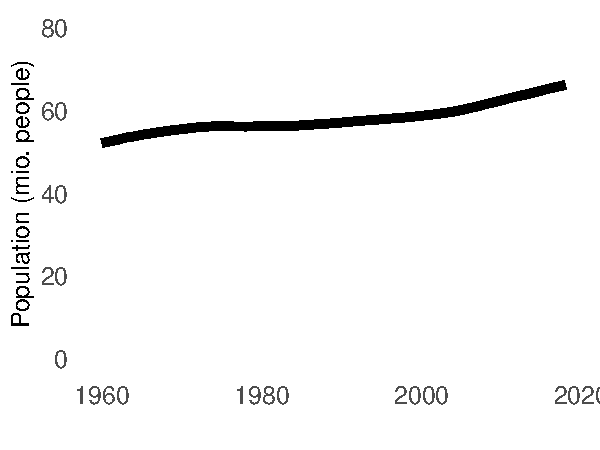
\includegraphics{book_files/figure-latex/fig1-1} 

}

\caption{\label{fig:figs}Population of the UK. Data Source: Eurostat}\label{fig:fig1}
\end{figure}

While the line chart above is a bit boring, Figure \ref{fig:fig2} is certainly not boring. It is very colourful and shows lots of data. This chart type is called a population pyramid chart. The chart shows the age composition of the global population. The width at the bottom of the chart represents the number of people in the youngest age group and the top the number of people in the oldest age group. Why do you think it is called a pyramid chart? And why do you think this version of the chart looks more like a cake? And finally, why is this trend both good and worrying for policy makers?

\begin{figure}

{\centering 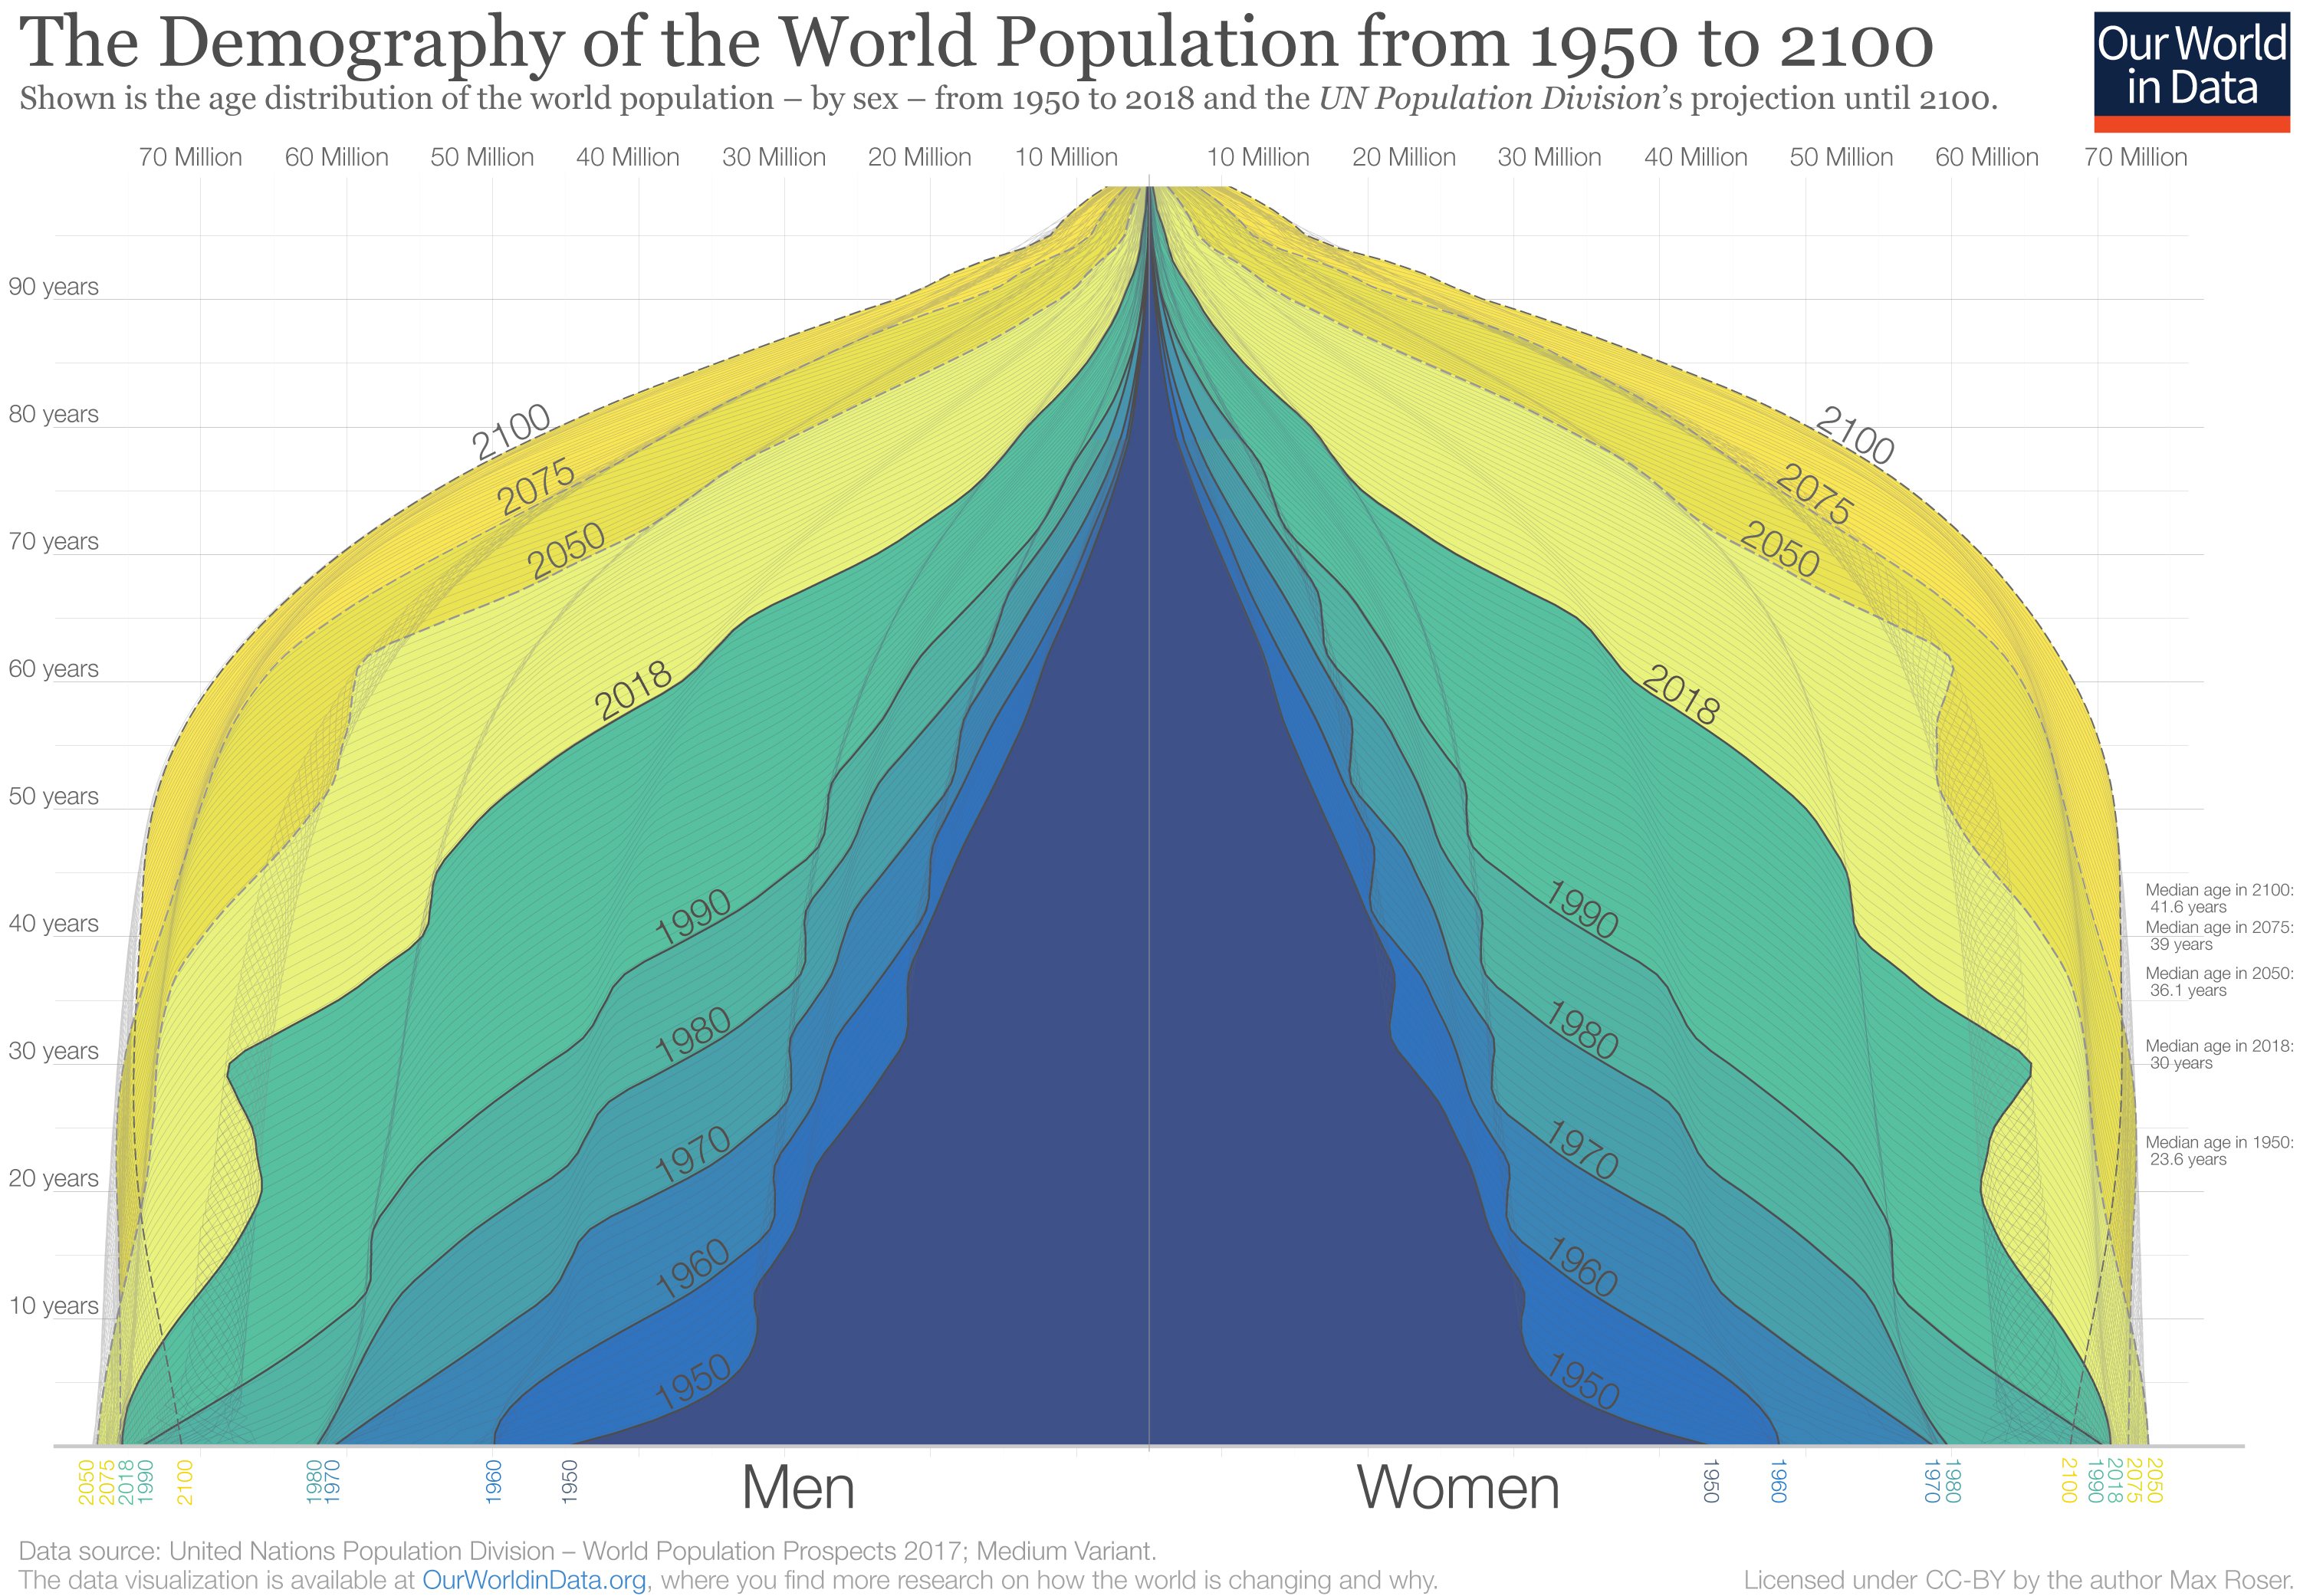
\includegraphics[width=0.8\linewidth]{_resources/chapter_people/poppyramid} 

}

\caption{Global Population Age Composition. Source: Our World in Data}\label{fig:fig2}
\end{figure}

Data on the number of people are important in itself but are also important ingredients in many other economics statistics. We therefore need to know how population levels are defined, how me measure population levels and and how we visualize data on population levels.

Let's get started.

\hypertarget{definitions-on-people}{%
\section{Definitions on people}\label{definitions-on-people}}

When we show and discuss data it is important that we agree on how we define the concept. We therefore begin by going through some definitions. Some of these definitions are not only limited to economic data. For example the definition on flow and stock variables, which we can use for any data type. Most of the definitions are fairly simple. That is actually the case for most definitions in this book. It is not the understanding of the definition that is challenging. The challenging part of working with economic data is knowing that there are definitions and that using a different definition can lead to a different conclusion about patterns in economic data.

\hypertarget{flow-and-stock-variables}{%
\subsection{Flow and stock variables}\label{flow-and-stock-variables}}

Variables either capture flows or stocks. We can illustrate flow and stock variables using a bathtub as in Figure \ref{fig:baththub}. The water level in the bathtub at a given point in time is a stock variable. The amount of water that has flown into the tub over a period of time is a flow variable.

\begin{figure}

{\centering 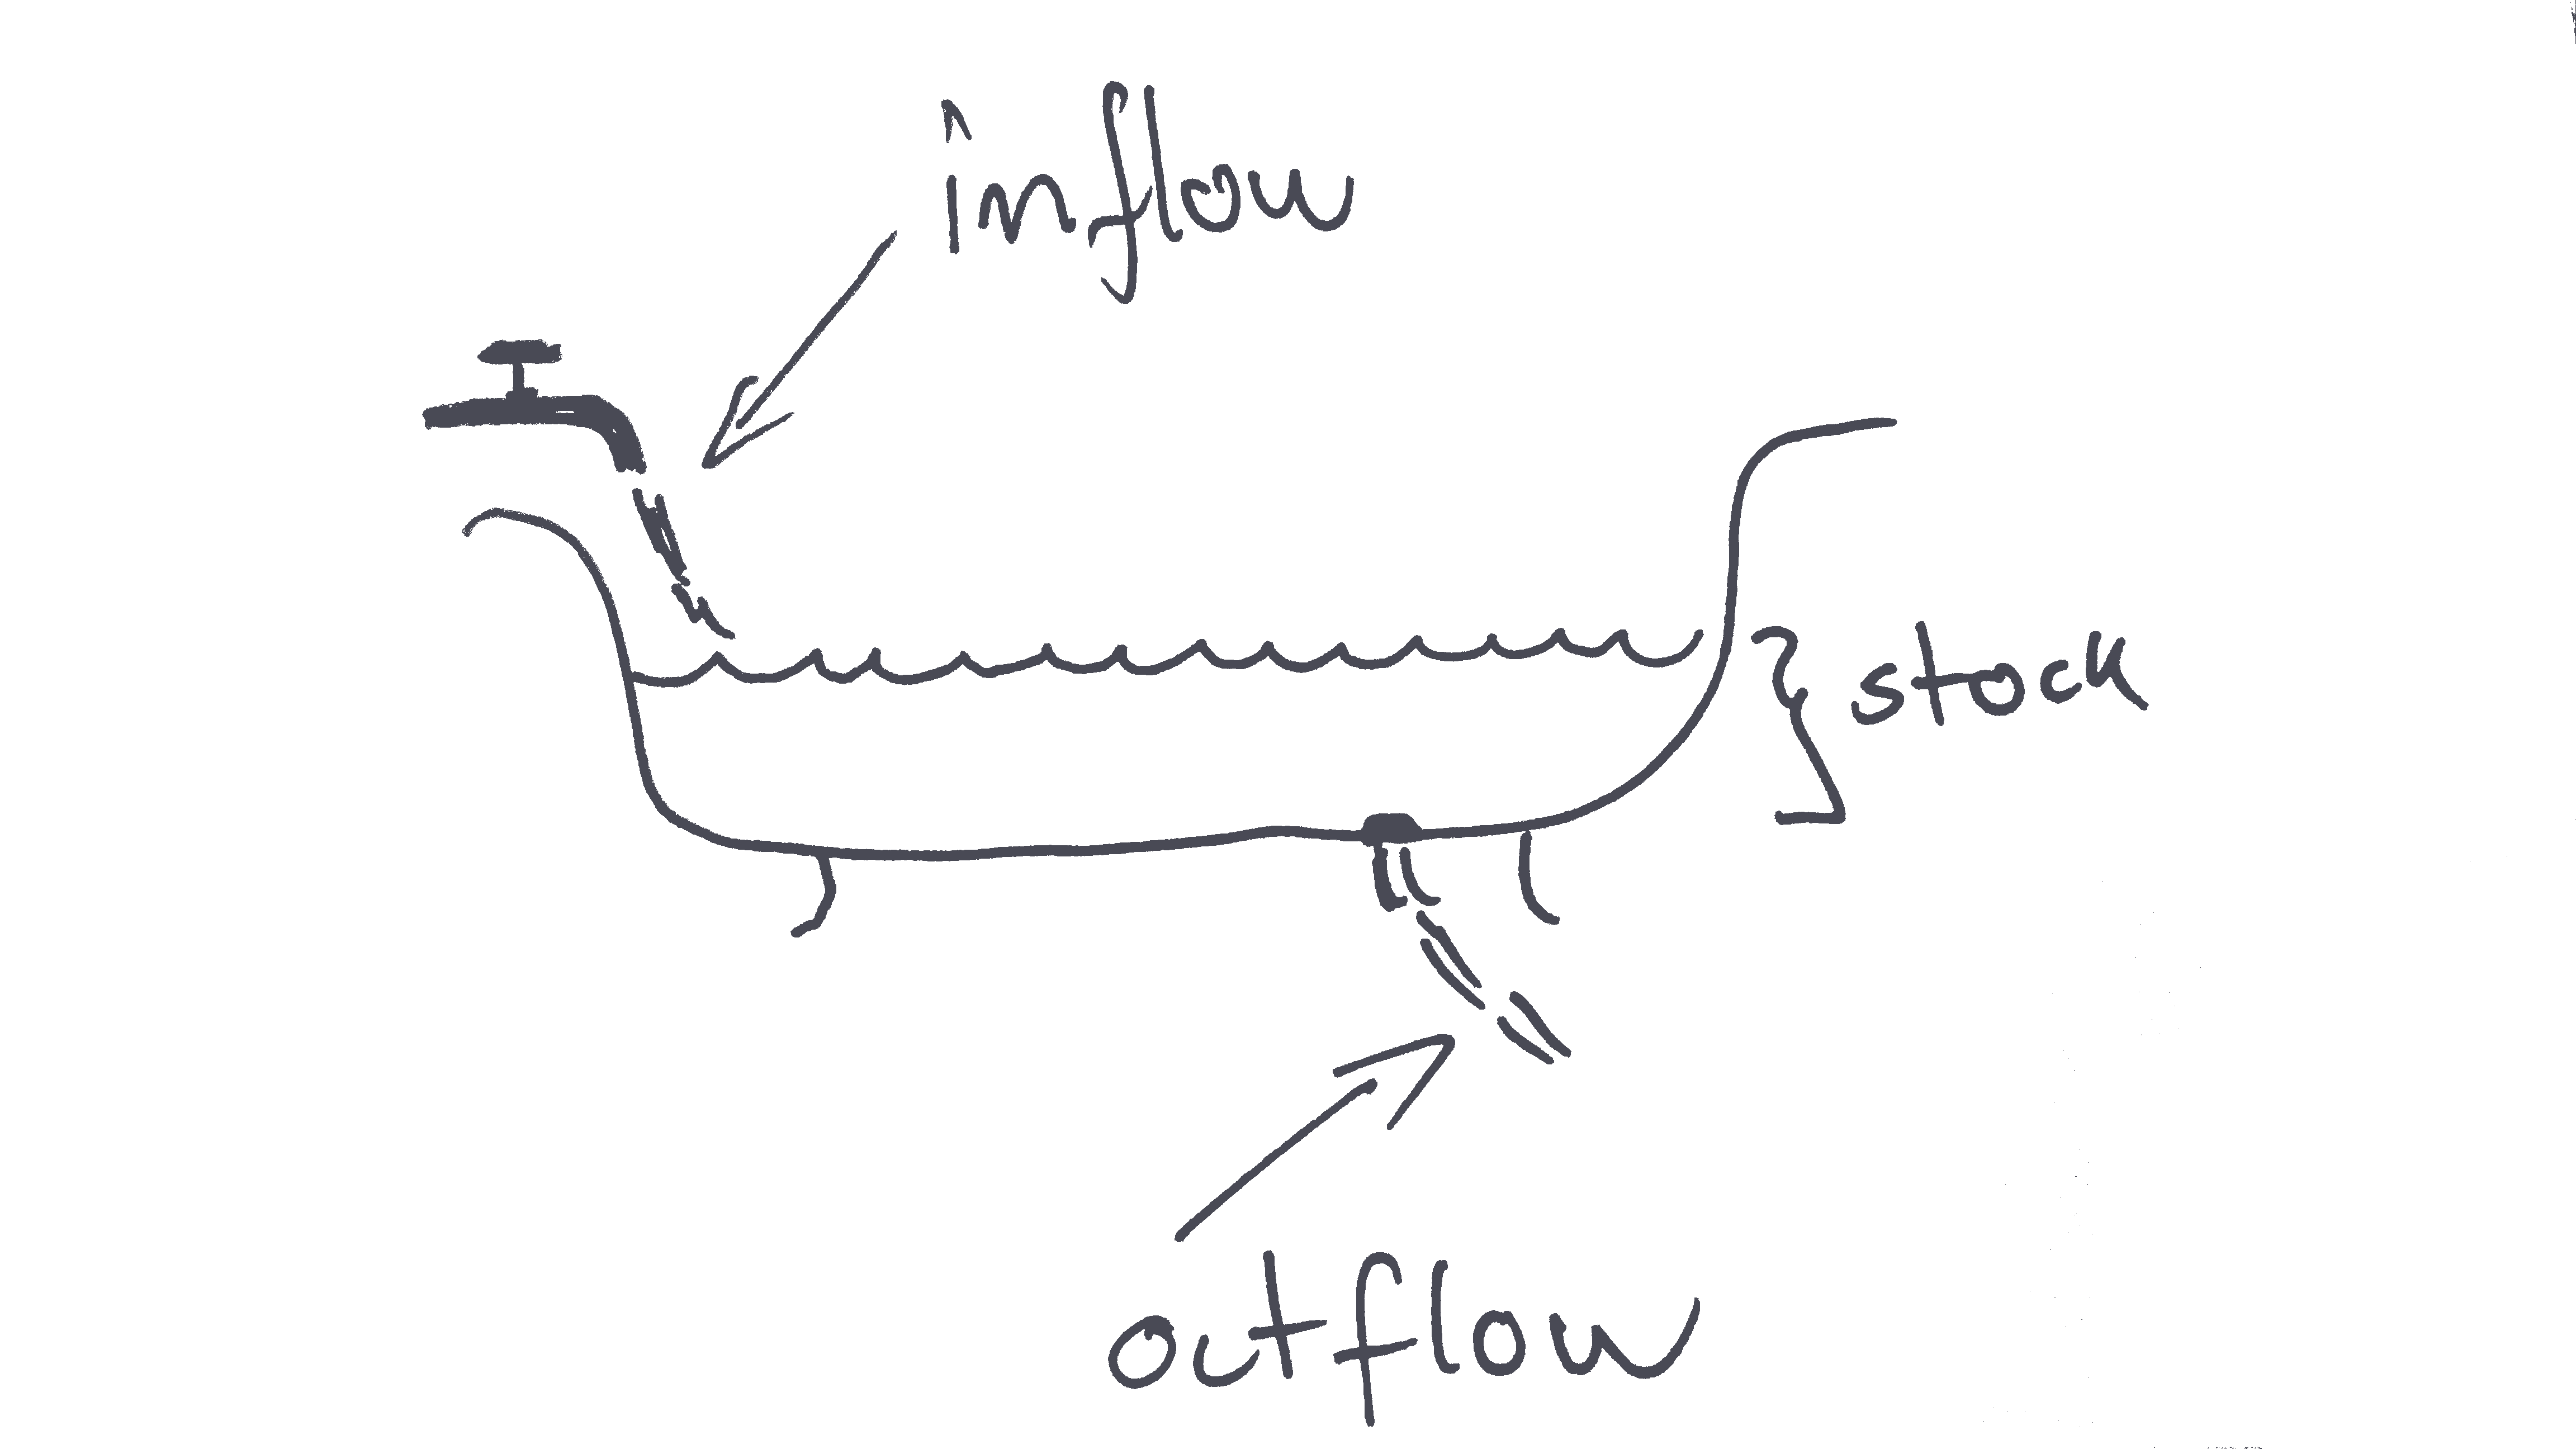
\includegraphics[width=0.9\linewidth]{_resources/chapter_people/flowbathtub} 

}

\caption{A bathtub with water illustrating flows and stocks}\label{fig:baththub}
\end{figure}

The easiest way to distinguish between flow and stock variables is that a flow variable is measured over a \emph{period} of time while stock variable is measured at a specific \emph{point} of time. If some asked you: ``How much water flowed into the bathtub on September 4 at 4:40pm and 10 seconds?'' It would be very difficult to answer. However, if someone asked ``How much water was in the bathtub on September 4 at 4:40pm and 10 seconds?'', it would be quite easy to answer (given that you had some tool to measure). This is because the water level is a stock variable. A stock variable is measured at a point in time and ``September 4, at 4:40pm and 10 seconds'' is a point in time. On the other hand if someone asked ``How much water flowed into the bathtub on September 4 between 4:40pm and 4:50pm?'', you would also be able to oanswer it, because you are now given a ``period of time'' (a period of 10 minutes) and flow variables are measured over a period.

\begin{myblock}
\textbf{Flow variable and stock variables}

\begin{itemize}
\tightlist
\item
  A \emph{flow} variable measures a flow of quantity over a
  \emph{period} of time.

  \begin{itemize}
  \tightlist
  \item
    For example the flow of migrants into the UK from January 1 2017 to
    December 31 2017.
  \end{itemize}
\item
  A \emph{stock} variable measures the level of quantity at a
  \emph{point} of time.

  \begin{itemize}
  \tightlist
  \item
    For example the number of people residing in the UK at January 1,
    2018.
  \end{itemize}
\end{itemize}
\end{myblock}

Let's think about economic variables instead of water and bathtubs. What would be an example of stock and flow variables? An example of a stock variable would be wealth. We measure wealth at a ``point in time''. An example of a flow variable would be income. We measure income over a period of time.

Why is it important to know whether a variable is a flow or stock variable? First, because it is useful when we want to understand the changes in a variable. The change in the water level of the bathtub (a stock variable) can be described by the inflow and outflow of water. The change in wealth (stock) is a function of income and consumption flows. Second, because the best way to visualize the data depends on the type of variable.

We can often describe the change in a stock variable by underlying flows:

\[ \Delta Stock=Stock_{1}-Stock_{0}=Flow_{0-1} \]

For example the change in the population level of the UK from 1 January, 2002 to 1 January, 2003 equals the number of people who immigrated to the UK, minus the number of people who left the UK (emmigrated), plus the number of children born, plus the number pof people who died in the period from 1 January, 2002 to 1 January 2003. In this example the population level is a stock variable. It is measured at a point in time (January 1, 2002). The other variables are all flow variables that are measured over a period of time. For example the number of births from 1 January 2002 to 1 January, 2003.

In the limit we would not be able to measure a flow variable as a stock variable. We could measure the number of people living in the UK on January 1, 2002 at five seconds and 3 milliseconds after 10:00AM, but how many children are born in exactly that millisecond? A child birth typically takes more than a second, so how do we allocate a birth a precise millisecond?

\hypertarget{the-population-level}{%
\subsection{The population level}\label{the-population-level}}

Let us now turn to a definition that we already discussed: The population.

\begin{myblock}
\textbf{The population level}

\begin{itemize}
\tightlist
\item
  The number of people in an area at a specific point in time.
\end{itemize}
\end{myblock}

In most cases we are interested in the number of people of \emph{living} in an area, but in some contexts it could be something else. For example the number of people \emph{working} in an area. For example the number of people working in Bristol (I work in Bristol, but I do not reside in Bristol).

The area could be a planet, a continent a country, a region, a county, a municipality, a house or any other clearly defined space.

\hypertarget{the-population-flows}{%
\subsection{The population flows}\label{the-population-flows}}

The population level of an area can change because of non-zero net migration flows and non-zero natural reproduction flows. These two concepts are defined below:

\begin{myblock}
\textbf{Migration flows}

\begin{itemize}
\tightlist
\item
  Immigration: the number of people entering an area over a period of
  time.
\item
  Emigration: the number of people leaving an area over a period of
  time.
\item
  Net migration: Immigration minus emigration
\end{itemize}
\end{myblock}

\begin{myblock}
\textbf{Natural reproduction flows}

\begin{itemize}
\tightlist
\item
  Deaths: the number of people in an area who died within a period of
  time.
\item
  Births: the number of people in an area who are born within a period
  of time.
\item
  Natural reproduction: The number of minus births the number of deaths.
\end{itemize}
\end{myblock}

What do we mean with non-zero? If the net migration flow is zero it means that the number of people who left the area equals the number of people who entered the area. In that case the population is unchanged. Only if the number of people leaving the area is not equal to the number of people entering the area can population levels change because of migration flows.

\hypertarget{people:vis}{%
\section{Visualizing population data}\label{people:vis}}

Having sorted out the basic definitions on population levels and the underlying flows in terms of net migration, births and deaths, we can now turn to the visualization of the population data. But how do we select the appropriate visualisation mode? We can generally split the data visualization process into three purposes:

\begin{enumerate}
\def\labelenumi{\arabic{enumi}.}
\tightlist
\item
  Exploratory data visualization
\item
  Analytical data visualization
\item
  Data visualization for communication.
\end{enumerate}

Let us say that we want to explore the data on the UK population. The first thing we might do is to download the data from the UK office for National Statistics and simply open it using the appropriate software such as MS Excel or R.

\hypertarget{exploring-data-on-population-levels}{%
\subsection{Exploring data on population levels}\label{exploring-data-on-population-levels}}

Let us first get some data from the website of the UK Office for National Statistics:

\begin{figure}

{\centering 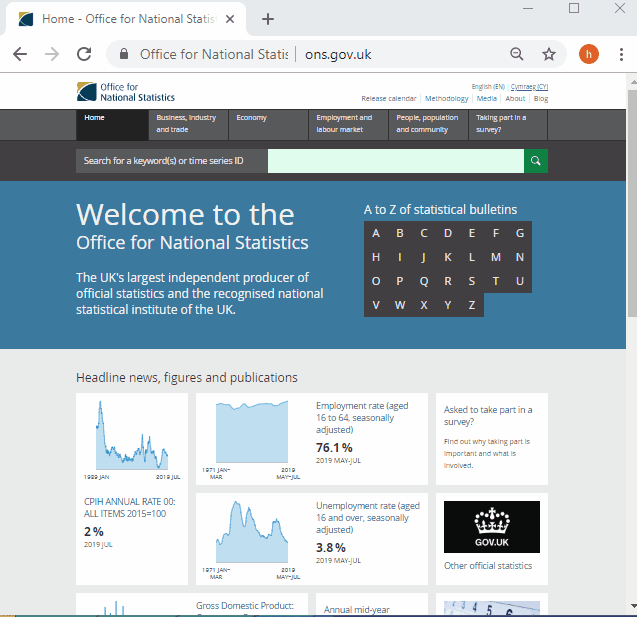
\includegraphics[width=0.7\linewidth]{_resources/chapter_people/gettingpopdata} 

}

\caption{Getting data from the ONS website}\label{fig:gettingdata}
\end{figure}

Now that we have the data, we are ready to look at the data. Figure \ref{fig:popdata} shows the sheet called ``MYE4'' of the downloaded file. This sheet contains ``Population estimates: Summary for the UK, mid-1971 to mid-2018''. That sounds about right.

\begin{figure}

{\centering 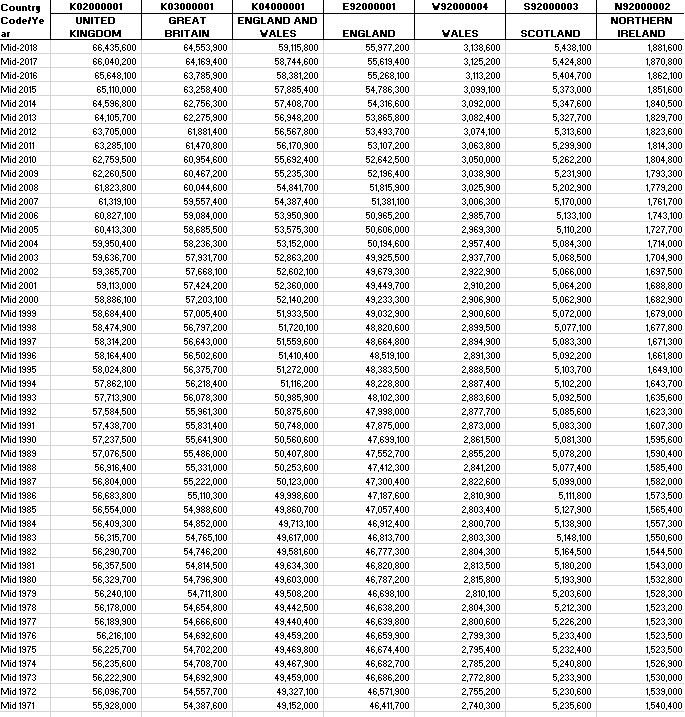
\includegraphics[width=0.6\linewidth]{_resources/chapter_people/table} 

}

\caption{UK population data opened in MS Excel}\label{fig:popdata}
\end{figure}

What do we learn from Figure \ref{fig:popdata}? First of all, that there are many numbers. Secondly, it looks a bit like the population is increasing in all regions. But overall it is really hard to tell. This is because a table is good for showing exact values, but with a lot of exact values we lose the overview.

\begin{figure}

{\centering 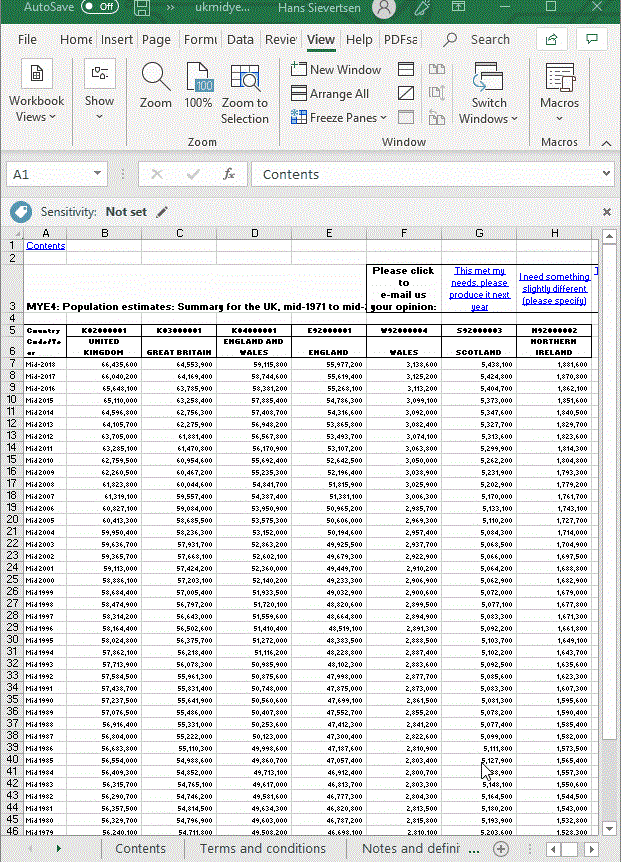
\includegraphics[width=0.6\linewidth]{_resources/chapter_people/visualisingdata1} 

}

\caption{Creating our first chart in MS Excel}\label{fig:firstchart}
\end{figure}

What can we learn from the chart created in \ref{fig:firstchart}? Not much. First of all, the chart indicates a decreasing trend. We typically read charts from left to right and almost all lines were decreasing. Secondly, it was very difficult to say anything about the population data for Wales, Scotland and Northern Ireland based on that chart, because the level is so low compared to England and the UK.

Let us solve the first problem first. Looking at the data again (see Figure \ref{fig:popdata} ), we observe that theONS puts the most recent value at the top. ``Mid-2018'' (i.e.~the point in time the stock variable is measured) is the first value, followed by ``Mid-2017'' and so on. That is not how Excel works. When we create charts in Excel, Excel will assume that the first value is the oldest value and the last value the most recent value. This is even more important when the values don't reflect dates that Excel might recognize. Excel will treat ``Mid-2018'' as any other name (just like ``Hans'', ``Julia'' and ``Jim''). And because we haven't told Excel anything else, it will just assume that we want to show the first value first (furthest to the left) and the last value last (furthest to the right). That sounds reasonable, or? So we first need to reorder the data. We can do this using the ``sort'' function in Excel as illustrated in Figure \ref{fig:sorted}.

\begin{figure}

{\centering 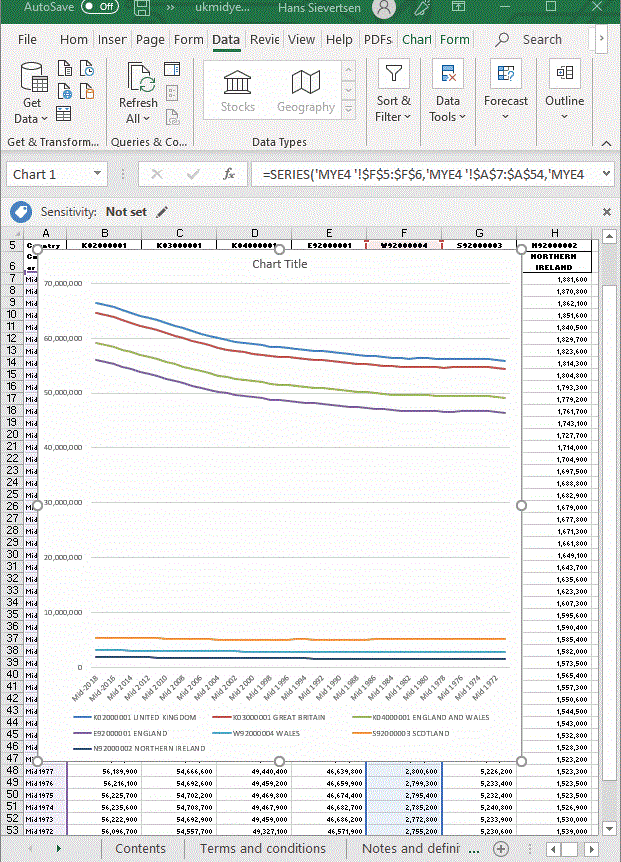
\includegraphics[width=0.7\linewidth]{_resources/chapter_people/sorted} 

}

\caption{Resorting the data}\label{fig:sorted}
\end{figure}

The new chart created in Figure \ref{fig:sorted} now shows the data in the right way. However, there is still the issue of the trends for the Northern Ireland, Wales and Scotland. Let us for now just concentrate on the UK and try to create a nice looking chart. In Figure \ref{fig:nicelooking} we create a chart that looks like \ref{fig:fig1}. It is a bit dull, but it only shows what it should show. The population level of the UK and how it developed over time. As the animation in \ref{fig:nicelooking} shows, creating a nice looking chart requires a lot of small adjustments in Excel. We adjust text color, font size, font type, line color, line width, axis colors, axis labels, titles and many other things. Adjusting all these aspects can be a bit tiresome, but they are important. Figure \ref{fig:fig1} is created using the software R. When creating charts with R, we can write a ``code'' that instructs R on how to create the chart. This can save a lot of time. Especially because we can reuse the code. We will hear more about R, but let us first think about how we could include population data for England, Scotland, Northern Ireland and Wales in one chart.

\begin{figure}

{\centering 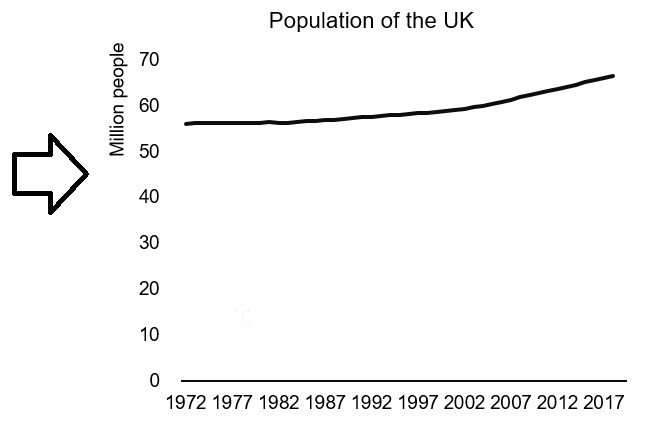
\includegraphics[width=0.5\linewidth]{_resources/chapter_people/nicechart} 

}

\caption{Creating our first nice looking chart using Excel. Data source: ONS.}\label{fig:nicelooking}
\end{figure}

The key problem is that England's population is a different level and that the y axis scale would be different if we only included Northern Ireland, Wales and Scotland and not England. What we can do is to create a second y axis. Let's have a go in Figure \ref{fig:nicelookingc}.

\begin{figure}

{\centering 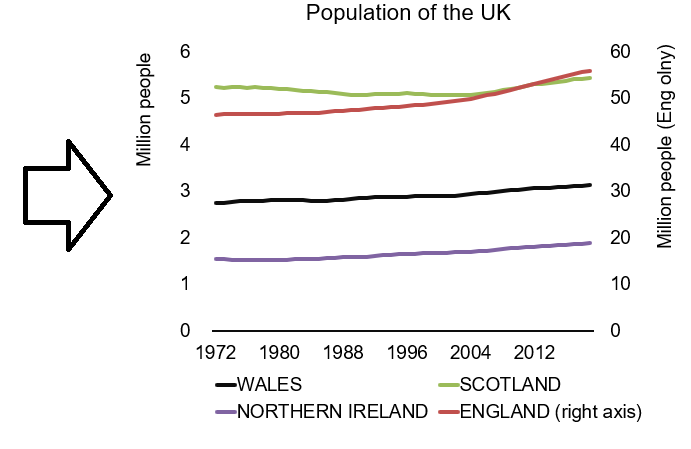
\includegraphics[width=0.5\linewidth]{_resources/chapter_people/nice1} 

}

\caption{Creating a chart of the population of the UK  using Excel. Data source: ONS.}\label{fig:nicelookingc}
\end{figure}

In the chart we create in Figure \ref{fig:nicelookingc} the population level of England is shown on the right axis, while the levels for the other countries are shown on the left axis. When using this strategy, it is very important to clearly state what axis each line belongs to. In the example above this could be improved. How would you improve that chart?

So far we just used the line chart. The line chart is one of the most popular chart types. How does it work?

\begin{itemize}
\tightlist
\item
  The chart shows the relationship between two variables.
\item
  The value of the first variable is reflected by the horizontal position.
\item
  The value of the second variable is reflected by the vertical position.
\item
  The values are connected along the horizontal axis suggesting that the variable is continuous.
\end{itemize}

Could we also use a different chart type to show the population of the UK? Yes, we could exploit that England, Nortern Ireland, Scotland and Wales are a part of a whole. Where the whole is the UK. We can use a stacked chart to show this. A stacked chart ``stacks'' the values on the vertical axis on top of each other. Stacking population levels for England, Wales, Northern Ireland and Scotland leads to the population of the UK. In Figure \ref{fig:stacked} we create a stacked area chart of the UK population. Now we do not need two axes. However, it is now much more difficult to identify the trends for the individual countries. This is a valuable lesson in data visualizations. We often have to sacrifice. We cannot show everything. We have to decide what the most important aspect of the data is.

\begin{figure}

{\centering 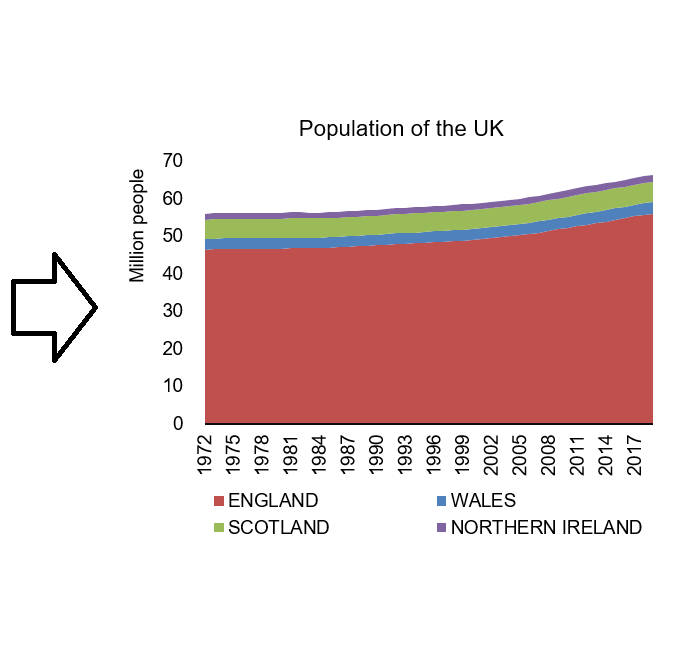
\includegraphics[width=0.5\linewidth]{_resources/chapter_people/stacked} 

}

\caption{Creating a stacked area chart for the UK population  using Excel. Data source: ONS.}\label{fig:stacked}
\end{figure}

An area chart works very much likes a line chart, with one important difference:

\begin{itemize}
\tightlist
\item
  The value is not simply reflected by the vertical and horizontal position, but by the size of the area.
\item
  We should therefore not truncate any of the axes (i.e.~make the shorter), because that would remove parts of the area.
\end{itemize}

\hypertarget{showing-relative-changes}{%
\subsection{Showing relative changes}\label{showing-relative-changes}}

What if the most important aspect of the population data is the relative change since 1971? We can see the changes in Figure \ref{fig:nicelookingc}, but it is not easy to compare the relative changes for the individual countries. To highlight the relative change in population levels since 1971 and allow us to compare across countries we can create an index. For all countries we readjust the values in such a way that the value in 1971 is 100 using the following formula:

\[ I_{year}=100\times \frac{Population_{year}}{Population_{1971}}\]

We use this formula on the data from the examples above in Figure \ref{fig:index}. From that chart we see that the population has increased the most in Northern Ireland and the least in Scotland, in relative terms. That was hard to see from the previous charts. However, now we cannot say anything about the levels anymore. This is because the level is ``canceled out'' in the index and only the relative changes remain.

\begin{figure}

{\centering 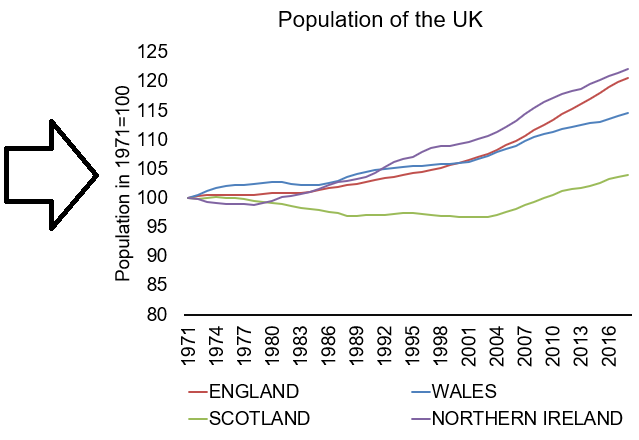
\includegraphics[width=0.5\linewidth]{_resources/chapter_people/index} 

}

\caption{Showing the relative population growth of the UK using an index in Excel. Data source: ONS.}\label{fig:index}
\end{figure}

\hypertarget{creating-a-table-on-population-changes}{%
\subsection{Creating a table on population changes}\label{creating-a-table-on-population-changes}}

Now what if we are only interested in the population level in 1971 and 2018 and how it changed. Could we show that in a different way that gives us access to more information? Yes, we could use a table because now it is only a few variables that needs to be shown. But designing a table also requires quite a bit of adjustment in Excel (or Word).

In Figure \ref{fig:tableb} we create a simple Table, but pay attention how we use black lines, borders, white space and text alignment to make the table as readable as possible.

\begin{itemize}
\tightlist
\item
  Solid black lines separate titles from main data and data levels from changes.
\item
  As numbers have the same width we can align the numbers and the text in the center.
\item
  We can now confirm the pattern from the index above, Northern Ireland experienced the largest growth in relative terms and Scotland the lowest.
\item
  Compared to the charts above we have precise information about both the levels and the changes.
\end{itemize}

\begin{figure}

{\centering 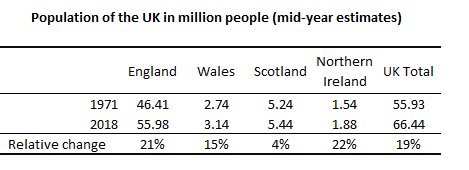
\includegraphics[width=0.5\linewidth]{_resources/chapter_people/tableb} 

}

\caption{Showing the population of the UK using a Table. Data source: ONS.}\label{fig:tableb}
\end{figure}

\hypertarget{describing-the-change-in-levels-by-the-underlying-flow-variables}{%
\subsection{Describing the change in levels by the underlying flow variables}\label{describing-the-change-in-levels-by-the-underlying-flow-variables}}

We can investigate the underlying population flows to get a better understanding of the dynamics that led to the change in the population levels we observed. Consider the change in the population of the UK from January 1 2015 to January 1 2016. We can decompose the change in the population level (a stock variable) by the following four flows:

\begin{itemize}
\tightlist
\item
  The population on January 1 2015

  \begin{itemize}
  \tightlist
  \item
    \(+\) moved to the country during 2015.
  \item
    \(-\) moved out of the country during 2015.
  \item
    =net migration
  \item
    \(+\) born the during 2015.
  \item
    \(-\)\} died the during 2015.
  \item
    (=natural population change)
  \end{itemize}
\item
  \(=\) The population on January 1 2016.
\end{itemize}

The Eurostat database provides data on the underlying flows in the population levels. The question is: how to best visualize this change? In Figure \ref{fig:popflows} we show the flows by means of stacked bars and the stocks in terms of a line chart. We thereby exploit that the total change is equal to the natural population change plus the net migration. One challenge with the latter approach (stacking bars and areas) is that if a series can contain both negative and positive values, it might be hard to read or even slightly misleading, because the negative or positive value is hidden. However, the overall pattern is clearly visible. In recent years, the population of the UK ihas increased a lot, and this is both due to positive net migration flows and postive reproduction flows.

\begin{figure}

{\centering 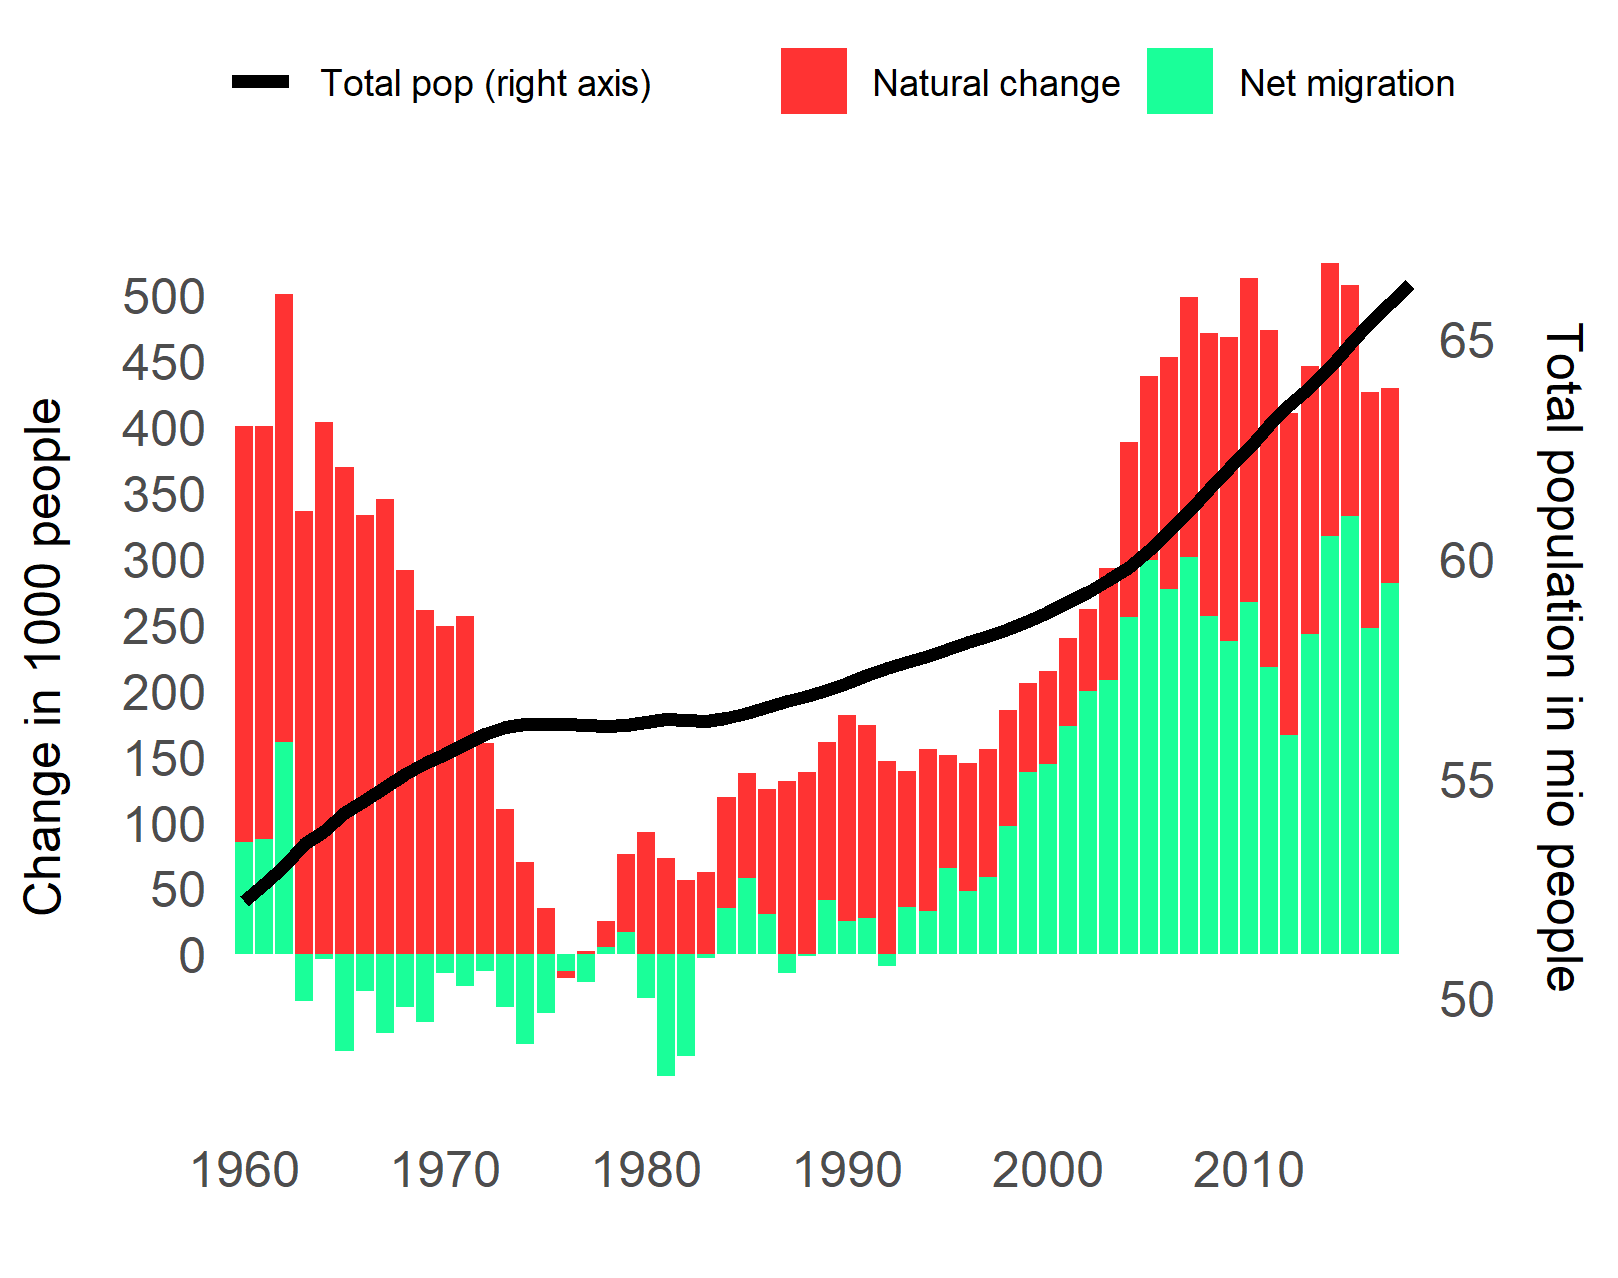
\includegraphics[width=0.8\linewidth]{_resources/chapter_people/fig7} 

}

\caption{Annual changes in the  population of the United Kingdom in terms of net migration (immigration minus emigration) and the natural population change (births minus deaths). Data source: Eurostat.}\label{fig:popflows}
\end{figure}

\hypertarget{creating-a-pyramid-chart-using-excel}{%
\subsection{Creating a pyramid chart using Excel}\label{creating-a-pyramid-chart-using-excel}}

We have now shown the basic levels and flows, can we also create more advanced charts in Excel? For example a chart like \ref{fig:fig2}?. The population pyramid chart. Yes. We can create a lot of charts using Excel. And a pyramid chart can be created with some creativity. Let's first consider the various aspects of this chart

\begin{itemize}
\tightlist
\item
  The width of the chart shows the number of people in a specific age group.
\item
  We split the chart by gender and show the number of men and women, respectively to the left and to the right.
\item
  The vertical position reflects the age group.
\end{itemize}

We can create this chart in Excel by creating a a bar chart. A bar chart is very similar to an area chart, we show the value in terms of the size of an area. However, in contrast to both the area and line chart, the values are not connected. This is very useful when values are not continuous. This is not the case here, but it it is good to keep this in mind. Figure \ref{fig:pyramid} shows how we can do it. Pay good attention to how we remove the minus.

\begin{figure}

{\centering 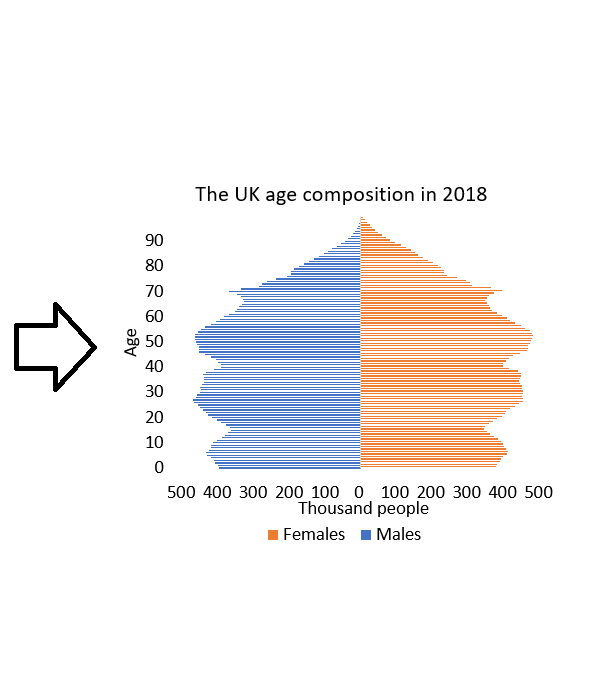
\includegraphics[width=0.8\linewidth]{_resources/chapter_people/pyramid} 

}

\caption{Showing the age composition of the UK population by gender. Data source: Eurostat. [Here is a video where I show how I created this chart in MS Excel.](https://youtu.be/AW7sdaJRbtc)}\label{fig:pyramid}
\end{figure}

\hypertarget{people:sum}{%
\section{Summary}\label{people:sum}}

So what should you take away from this chapter?

\begin{itemize}
\tightlist
\item
  The difference between a stock and a flow variable
\item
  Advantages of Tables vs.~Charts
\item
  How we measure the population level and migration and reproduction flows.
\item
  Creating basic charts and tables in Excel
\item
  Creating a pyramid chart in Excel
\item
  Using and interpreting an Index with one variable.
\end{itemize}

\hypertarget{activity}{%
\chapter{Data about economic activity}\label{activity}}

\hypertarget{about-this-chapter-1}{%
\section{About this chapter}\label{about-this-chapter-1}}

This chapter is about visualizing and describing data on economic activity. Economic activity is measured in the System of National Accounts (SNA) and conceptualized by the Gross Domestic Product, (GDP). We will not cover the SNA in detail.\footnote{For details on the SNA, please visit the following \href{https://unstats.un.org/unsd/nationalaccount/sna.asp}{website}} It is basically a set of rules and instructions that have been agreed internationally to ensure that measures of economic activity are comparable across countries. However, we will go through some of the key \emph{aggregegates} of the SNA (for example GDP, Gross National Income, the GDP inflator etc.). An aggregate is a measure that \emph{aggregates} several underlying variables. This chapter is mainly about the GDP, but we will also briefly touch upon other aggregates of the SNA as well as what the GDP is used for.

\hypertarget{intended-learning-outcomes-1}{%
\subsection{Intended learning outcomes}\label{intended-learning-outcomes-1}}

After reading this chapter you should be able to:

\begin{itemize}
\tightlist
\item
  Explain what the gross domestic product (GDP) is and calculate it.
\item
  Explain the three ways to measure GDP

  \begin{enumerate}
  \def\labelenumi{\arabic{enumi}.}
  \tightlist
  \item
    The Income Approach
  \item
    The Expenditure Approach
  \item
    The Output approach.
  \end{enumerate}
\item
  Explain what The gross national income (GNI) is and calculate it.
\item
  Calculate GDP per person and productivity.
\item
  Visualize data on economic activity.
\end{itemize}

\hypertarget{a-brief-history-of-gdp}{%
\subsection{A brief history of GDP}\label{a-brief-history-of-gdp}}

Most texts about the history of GDP start around the Great Depression in the 1930ies United States. The U.S. Congress realized that the economy was not running as well as it could, but had a hard time quantifying it. To the rescue came the economist Simon Kusnets who presented a report on the ``National Income, 1929-1935'' for the Congress (see \ref{fig:gdp1}), where he presented the idea of capturing the entire production, income and expenditure of the economy. And so the GDP was born. This story of how the GDP was created is probably the most well-known story of the GDP, but in reality the story of GDP is more complicated.

\begin{figure}

{\centering 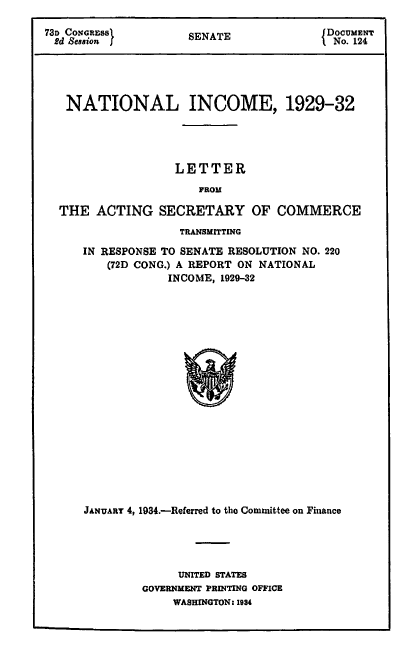
\includegraphics[width=0.65\linewidth]{_resources/chapter_gdp/kusnetz} 

}

\caption{Kusnets' report for the U.S. Congress, 1934. Source:  [Fraser St. Louis FED](fraser.stlouisfed.org/title/971).}\label{fig:gdp1}
\end{figure}

The idea of quantifying the size of the economy probably goes back to at least the 17th century. The exact definition of GDP has since then been redefined and adjusted. It is actually continuesly adjusted. More on that later. Giving Simon Kusnets a lot of credit for the GDP is not completely wrong. He refined the concept a lot and his report made it prominent. However, it wasn't until much later that it became the ``statistic to rule them all''.

The GDP as a concept is critisized a lot. The most prominent critisism is probably the ``Report by the Commission on the Measurement of Economic Performance and Social Progress'' published in Autumn 2009 by the economists Joseph Stiglitz, Amartya Sen and Jean-Poul Fitoussi. What is the key critisism of GDP? The main problem with the GDP is not so much the GDP itself, but more the misuse of GDP as a measure of well-being or welfare. Simon Kusnets was actually already aware of some of these issues and the potential misue of GDP. Figure \ref{fig:gdp1} shows a small section of the 273 page long report by Kusnetz.

Figure \ref{fig:gdp2} shows extracts of pages 5-7 in Kusnets original report \citep{kuznets1934national}. Kusnets made several points that are at the heat of the disucssion today, for example that ``With quantitative measurements especially, the definiteness of the result suggests, often misleadingly, a precision and simplicity in the outlines of the object measured.'' and ``Economic welfare cannot be adequately measured unless the personal distribution of income is known. And no income measurement undertakes to estimate the reverse side of income, that is, the intensity and unpleasantness of effort going into the earning of income.''

\begin{figure}

{\centering 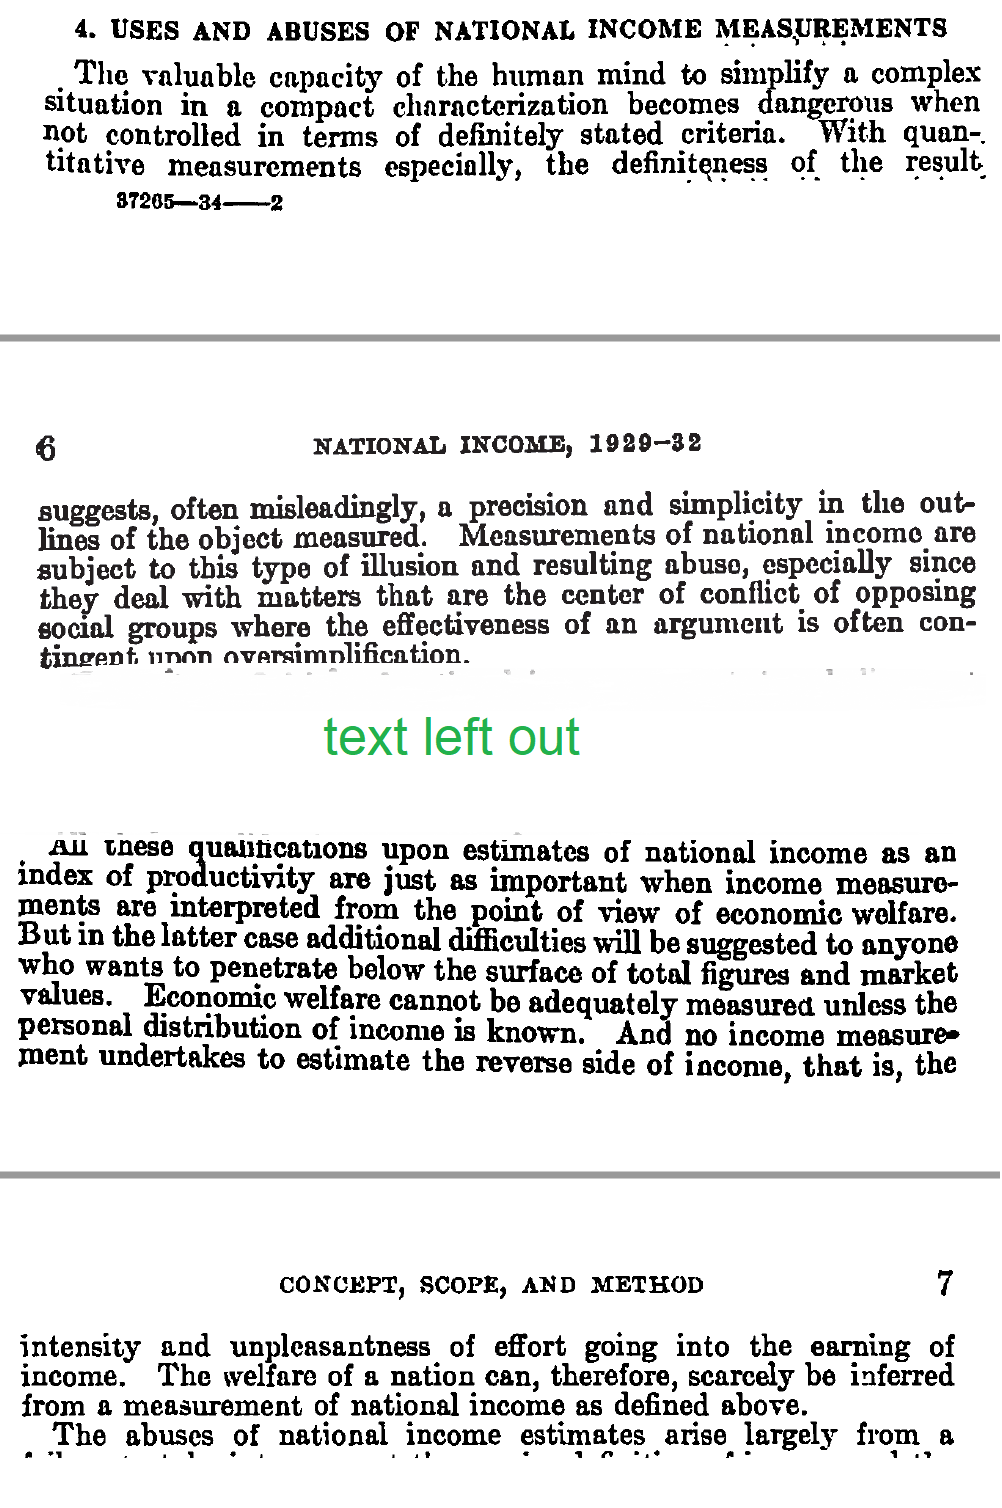
\includegraphics[width=0.7\linewidth]{_resources/chapter_gdp/kusnetz2} 

}

\caption{Page 5-7 in 'National Income, 1929–1932'. 73rd US Congress, 2d session, Senate document no. 124, 1934. Source:  [Fraser St. Louis FED](fraser.stlouisfed.org/title/971). }\label{fig:gdp2}
\end{figure}

So why should we care about GDP if it is no good? Actually it is a quite good of economic activity. But it is simply a measure of economic activity. We will return to the criticism of GDP in later chapters, but here we will discuss what it actually captures. When we know what the GDP measures, we can say more about what it doesn't measure and how we should and should not use it. After reading this chapter, you should be able to

\hypertarget{the-economy-of-microcountry}{%
\section{The Economy of Microcountry}\label{the-economy-of-microcountry}}

Let me introduce a very small country. It is not my home country, Denmark, but a country that is even smaller: Microcountry. Microcountry is just next to Neighbourcountry. Microcountry is so small that I can explain all economic activity in this country to you.

In this country we have one farm that produces flour. The farm sells the flour to a bakery for 10 £. To produce the flour, the farm has workers, and these workers earn a wage of 8 £. Finally, the farm pays a tax to the government of 2 £.

The bakery produces bread based on labor inputs in terms workers and the flour bought from the farm. The workers at the bakery receive 14 £ in wages, and the government receives 2 £ in taxes from the bakery. The bakery sells bread for 18 £ to the households in Microcountry. The households of Neighbourcountry buy bread from the bakery in Microcountry for 9 £, and the bakery in Microcountry is actually owned by residents of Neighbourcountry.

The households in Microcountry work for the bakery, the farm and for the government. They pay 1 £ in taxes to the government, and buy bread for 18 £ at the bakery. The households also import goods from Neighbourcountry for a value of in total 8 £. The government provides health service for the society of Microcountry and spends 5 £ in wages to be able to supply this service.

Now the big questions are:

\begin{itemize}
\tightlist
\item
  The Gross Domestic Product (GDP) of Microcountry?
\item
  The Gross National Income (GNI) of Microcountry?
\end{itemize}

To answer this we need to know what GDP is and how we can measure it.

\hypertarget{what-is-gdp-and-how-do-we-measure-it}{%
\section{What is GDP and how do we measure it?}\label{what-is-gdp-and-how-do-we-measure-it}}

The Gross Domestic Product captures the economic activity of an economy. What is economic activity? Just think of when you are economically active:

\begin{enumerate}
\def\labelenumi{\arabic{enumi}.}
\tightlist
\item
  When you go shopping and spend money.
\item
  When you work and receive a wage income.
\item
  When you create a product and sell it to someone.
\end{enumerate}

These three examples of how we as individuals are economically active actually capture the three ways we measure the Gross Domestic Product. The expenditure approach, the income approach and the output approach. Let us now discuss these approaches in detail. The GDP captures how much is spend, how much is produced or how much is earned within a period. It is therefore a flow variable.

Below is a short animation of what the GDP is, created by the UK Treasury.

\begin{verbatim}
## PhantomJS not found. You can install it with webshot::install_phantomjs(). If it is installed, please make sure the phantomjs executable can be found via the PATH variable.
\end{verbatim}

\label{fig:whatisgdp}What is GDP?. Source: HM Treasury.

\hypertarget{the-expenditure-approach}{%
\subsection{The Expenditure Approach}\label{the-expenditure-approach}}

The \emph{expenditure} approach (called the spending approach in \citep{core}) measures the GDP in terms of expenditures by households and the Government, as well investments and net exports of goods and services (i.e.~exports minus imports). All these expenditures are summarized in the following equation:
\begin{align}
   \text{GDP}^{\text{E}} \text{=Y=C+G+I+X-M}
\end{align}
where:

\begin{itemize}
\tightlist
\item
  \textbf{Y} is the Gross Domestic Product (GDP).
\item
  \textbf{C} is final consumption of goods and services by households. It includes goods like food, cars, and clothing, as well as services such as hotel stays.
\item
  \textbf{G} is final consumption expenditure of goods and services by the government.
\item
  \textbf{I} is investments (also called gross capital formation) are investments in fixed assets such as machinery, buildings etc.
\item
  \textbf{X} is goods and services produced domestically but consumed abroad (Exports)
\item
  \textbf{M} is goods and services produced abroad and consumed domestically (Imports).
\end{itemize}

Using data from the OECD, Figure \ref{fig:gdp3} shows the size of each element of the expenditure approach for the United Kingdom over the period 2000 to 2015. In Figure \ref{fig:gdp3} A, the development is shown in current prices. A change in the value from year to year is therefore a combination of a change in prices and a change in volume. We could have the extreme case, where we actually bought exactly the same quantity in all these years, but because the price increased, we would get the pattern shown in Figure \ref{fig:gdp3}. However, this is clearly not the case in the United Kingdom over this period. As Figure \ref{fig:gdp3} B shows, the values also increased in \emph{real} terms. In Figure \ref{fig:gdp3} B we used the GDP deflator to adjust the values in current prices (shown in A) to the 2017 price level.

\begin{figure}

{\centering 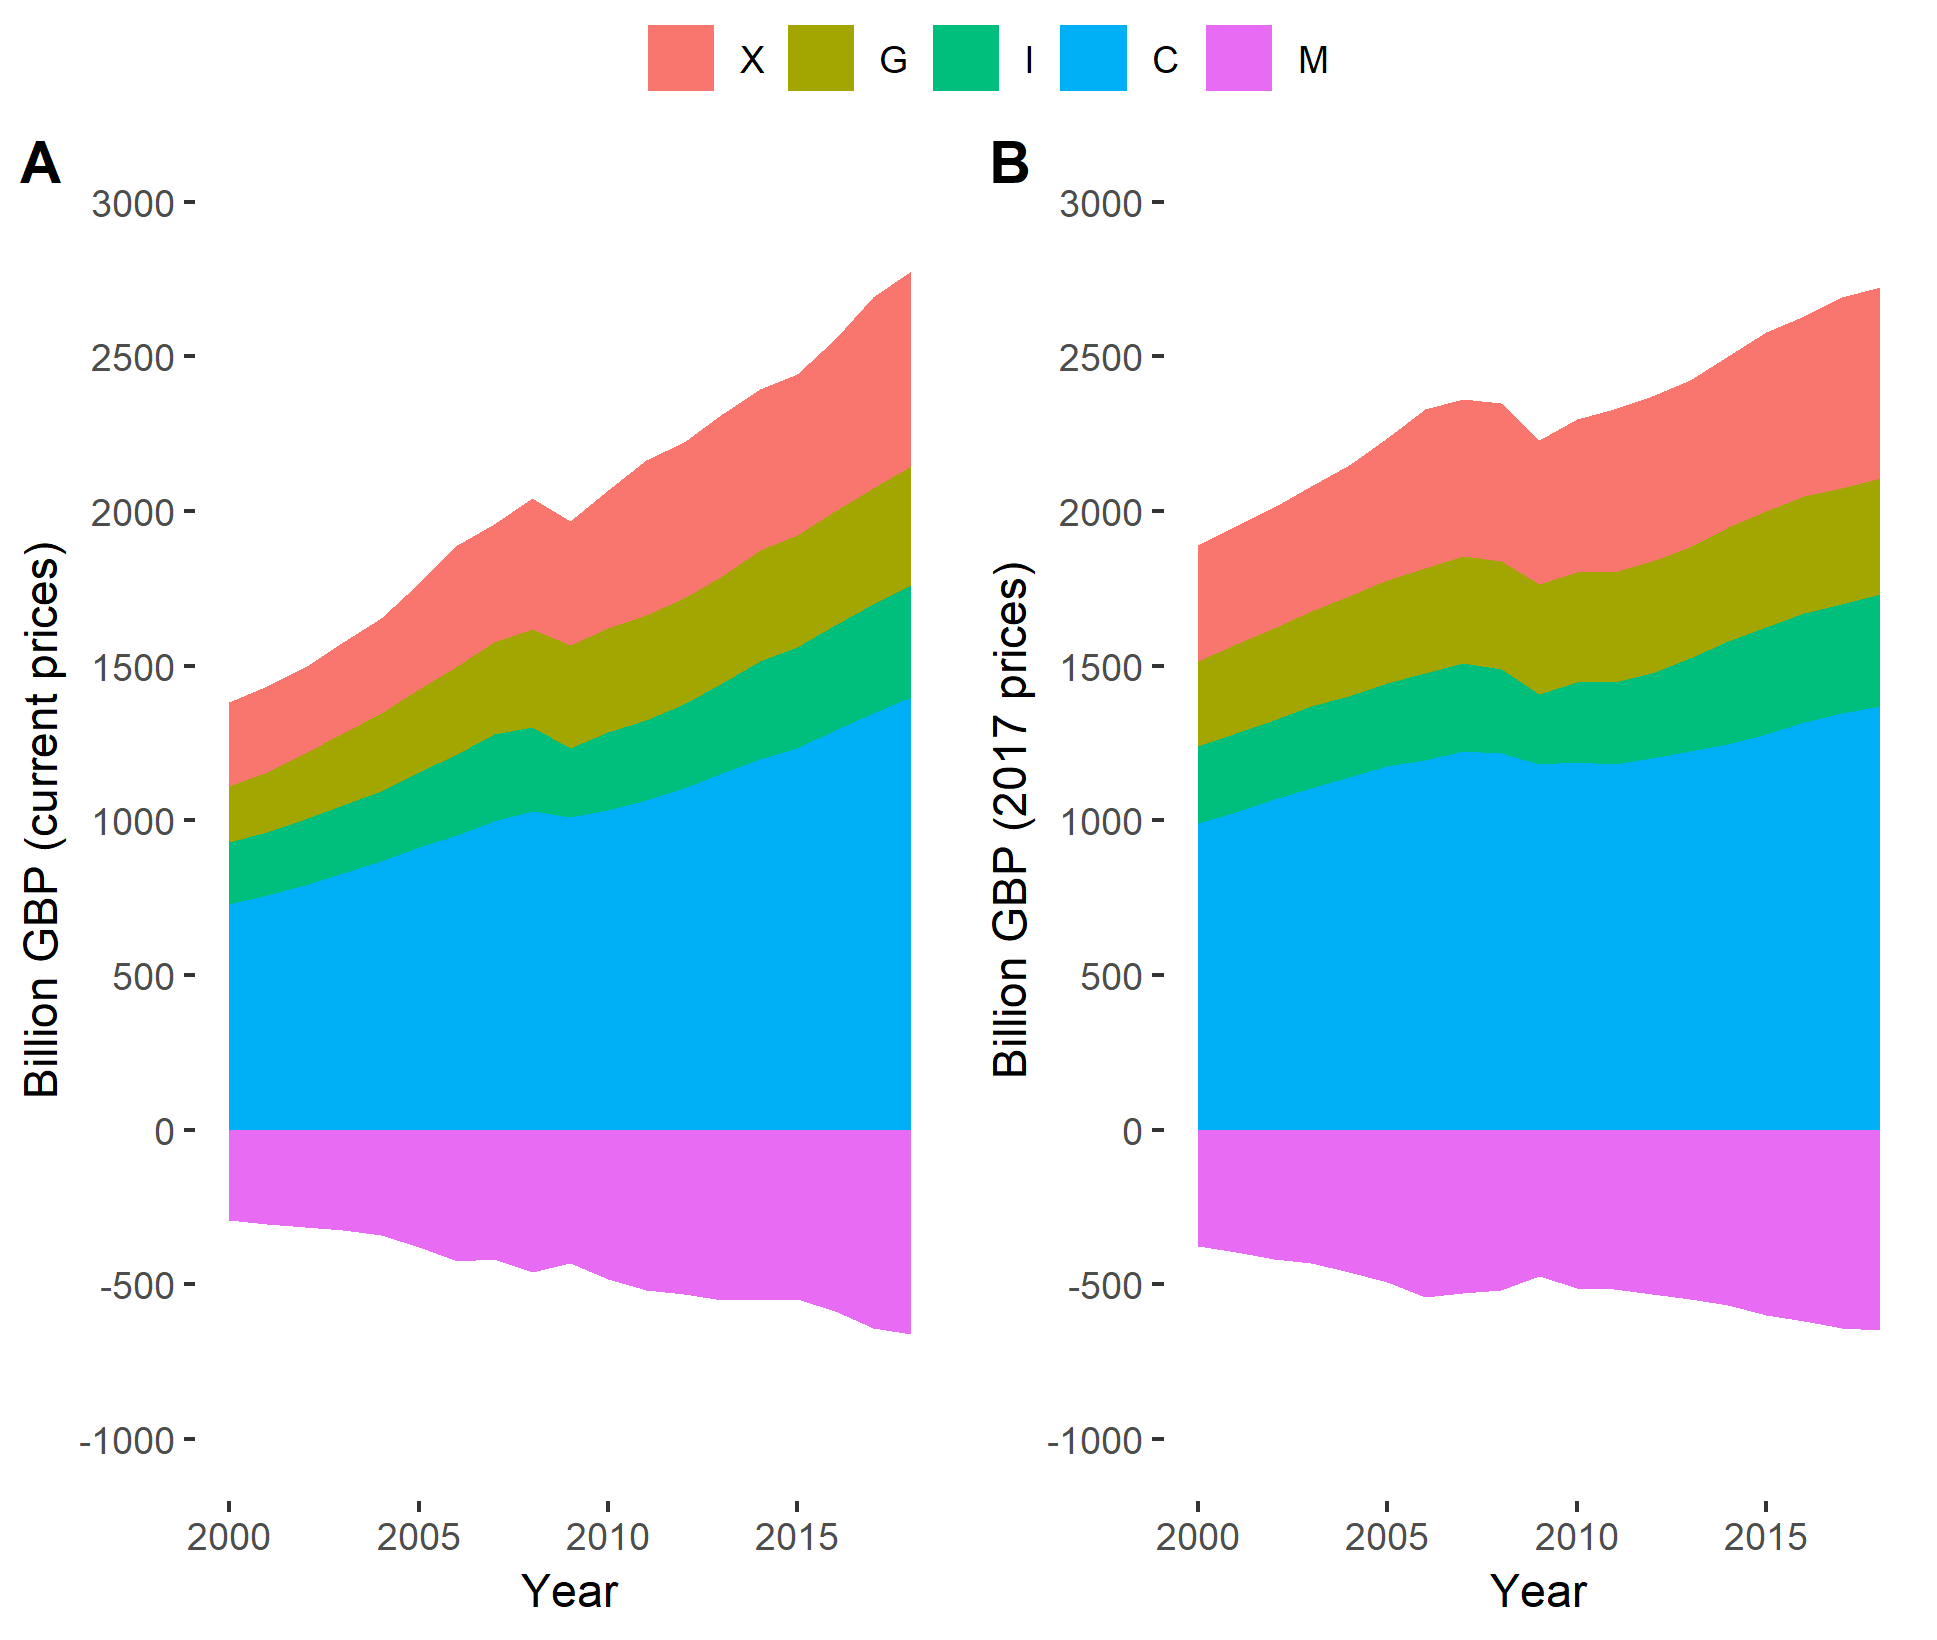
\includegraphics[width=0.9\linewidth]{_resources/chapter_gdp/fig1} 

}

\caption{The expenditure approach components of the Gross Domestic Product for the United Kingdom using a stacked area chart. **This is an example of an inappropriate chart type!** Imports enter negatively. Data source: OECD. Values are converted to the 2017 price level using the GDP deflator for each category.}\label{fig:gdp3}
\end{figure}

The charts in Figure \ref{fig:gdp3} are stacked area charts. As you might recall from the chapter on measuring people, area charts shows the size of the value by the size of the area and we are then putting each category on top of each other. This seems like a good solution with data on parts that constitute a ``whole'', such as the population of the Wales, Northern Ireland, Scotland and UK, that constitute the population of the UK.

Is it also a good idea to use stacked area charts to show the expenditure parts of GDP like in Figure \ref{fig:gdp3}? \textbf{No! The stacked area chart is not appropriate in this case!} Because the GDP by expenditure approach involves both negative and positive values, the stacked area chart does not work well Moreover, we are tempted to conclude that all categories increased in real (absolute) terms (i.e.~in volumes) over the period 2000 to 2018. But for all categories, except the first one, it is very difficult to see, because the all changes in the first category will map over in the following category. Government consumption (G) has for example been steadily increasing over the period. There was no drop over the financial crisis. But this is very hard to see from Figure \ref{fig:gdp3}.

It is much easier to identify the changes in individual series by means of a simple line chart, as shown in Figure \ref{fig:gdp4}. From Figure \ref{fig:gdp4} B we clearly see that Imports, Exports, Private Consumption and Investments suffered a drop in real values during the financial crisis, but Government Consumption did not. Both Figures \ref{fig:gdp3} and \ref{fig:gdp4} illustrate that Private Consumption (C) is the largest component of GDP in terms of the expenditure approach.

\begin{figure}

{\centering 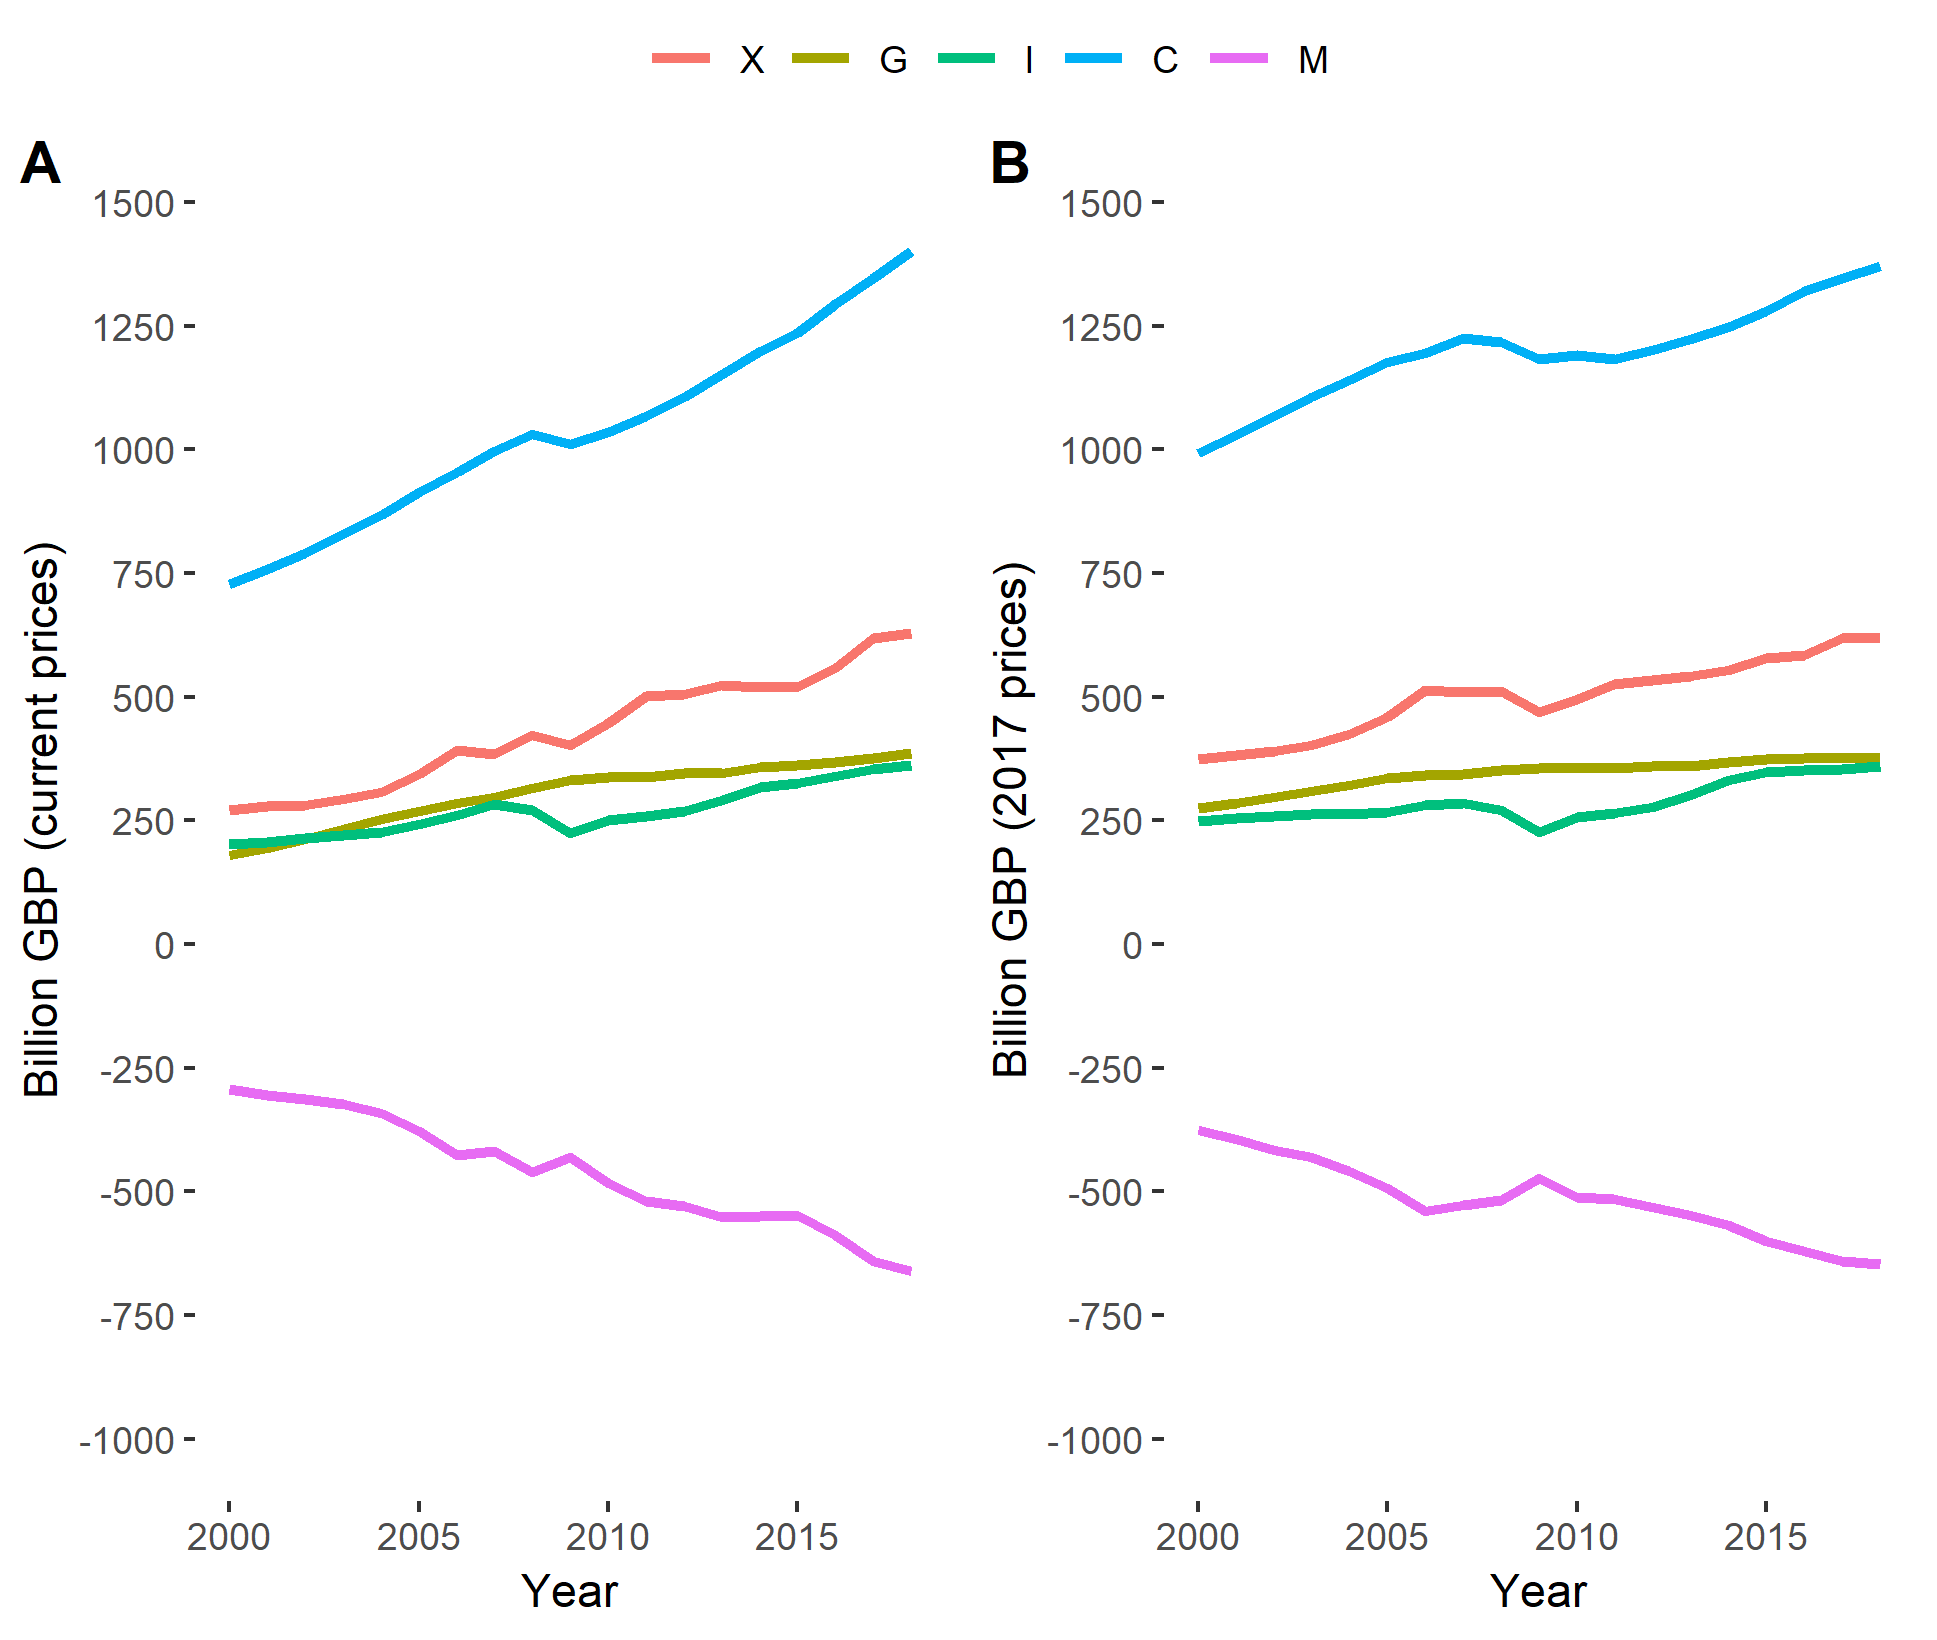
\includegraphics[width=0.9\linewidth]{_resources/chapter_gdp/fig2} 

}

\caption{The expenditure approach components of the Gross Domestic Product for the United Kingdom using line charts. Data source: OECD. Values are converted to the 2017 price level using the GDP deflator for each category}\label{fig:gdp4}
\end{figure}

Figure \ref{fig:gdp5} shows a line chart of the relative change in each component of the expenditure approach by means of an index, where the base value is the value in the year 2000. This figure also highlights the importance of adjusting for price changes. In terms of nominal values (in other words in current prices), the values increased by up to more than 200 percent over the period (as Figure \ref{fig:gdp5} A shows), but in real terms the change is much more modest (as Figure \ref{fig:gdp5} B shows). The Figure also shows that the relative drop over the financial was remarkable in terms of the Investments (I).

\begin{figure}

{\centering 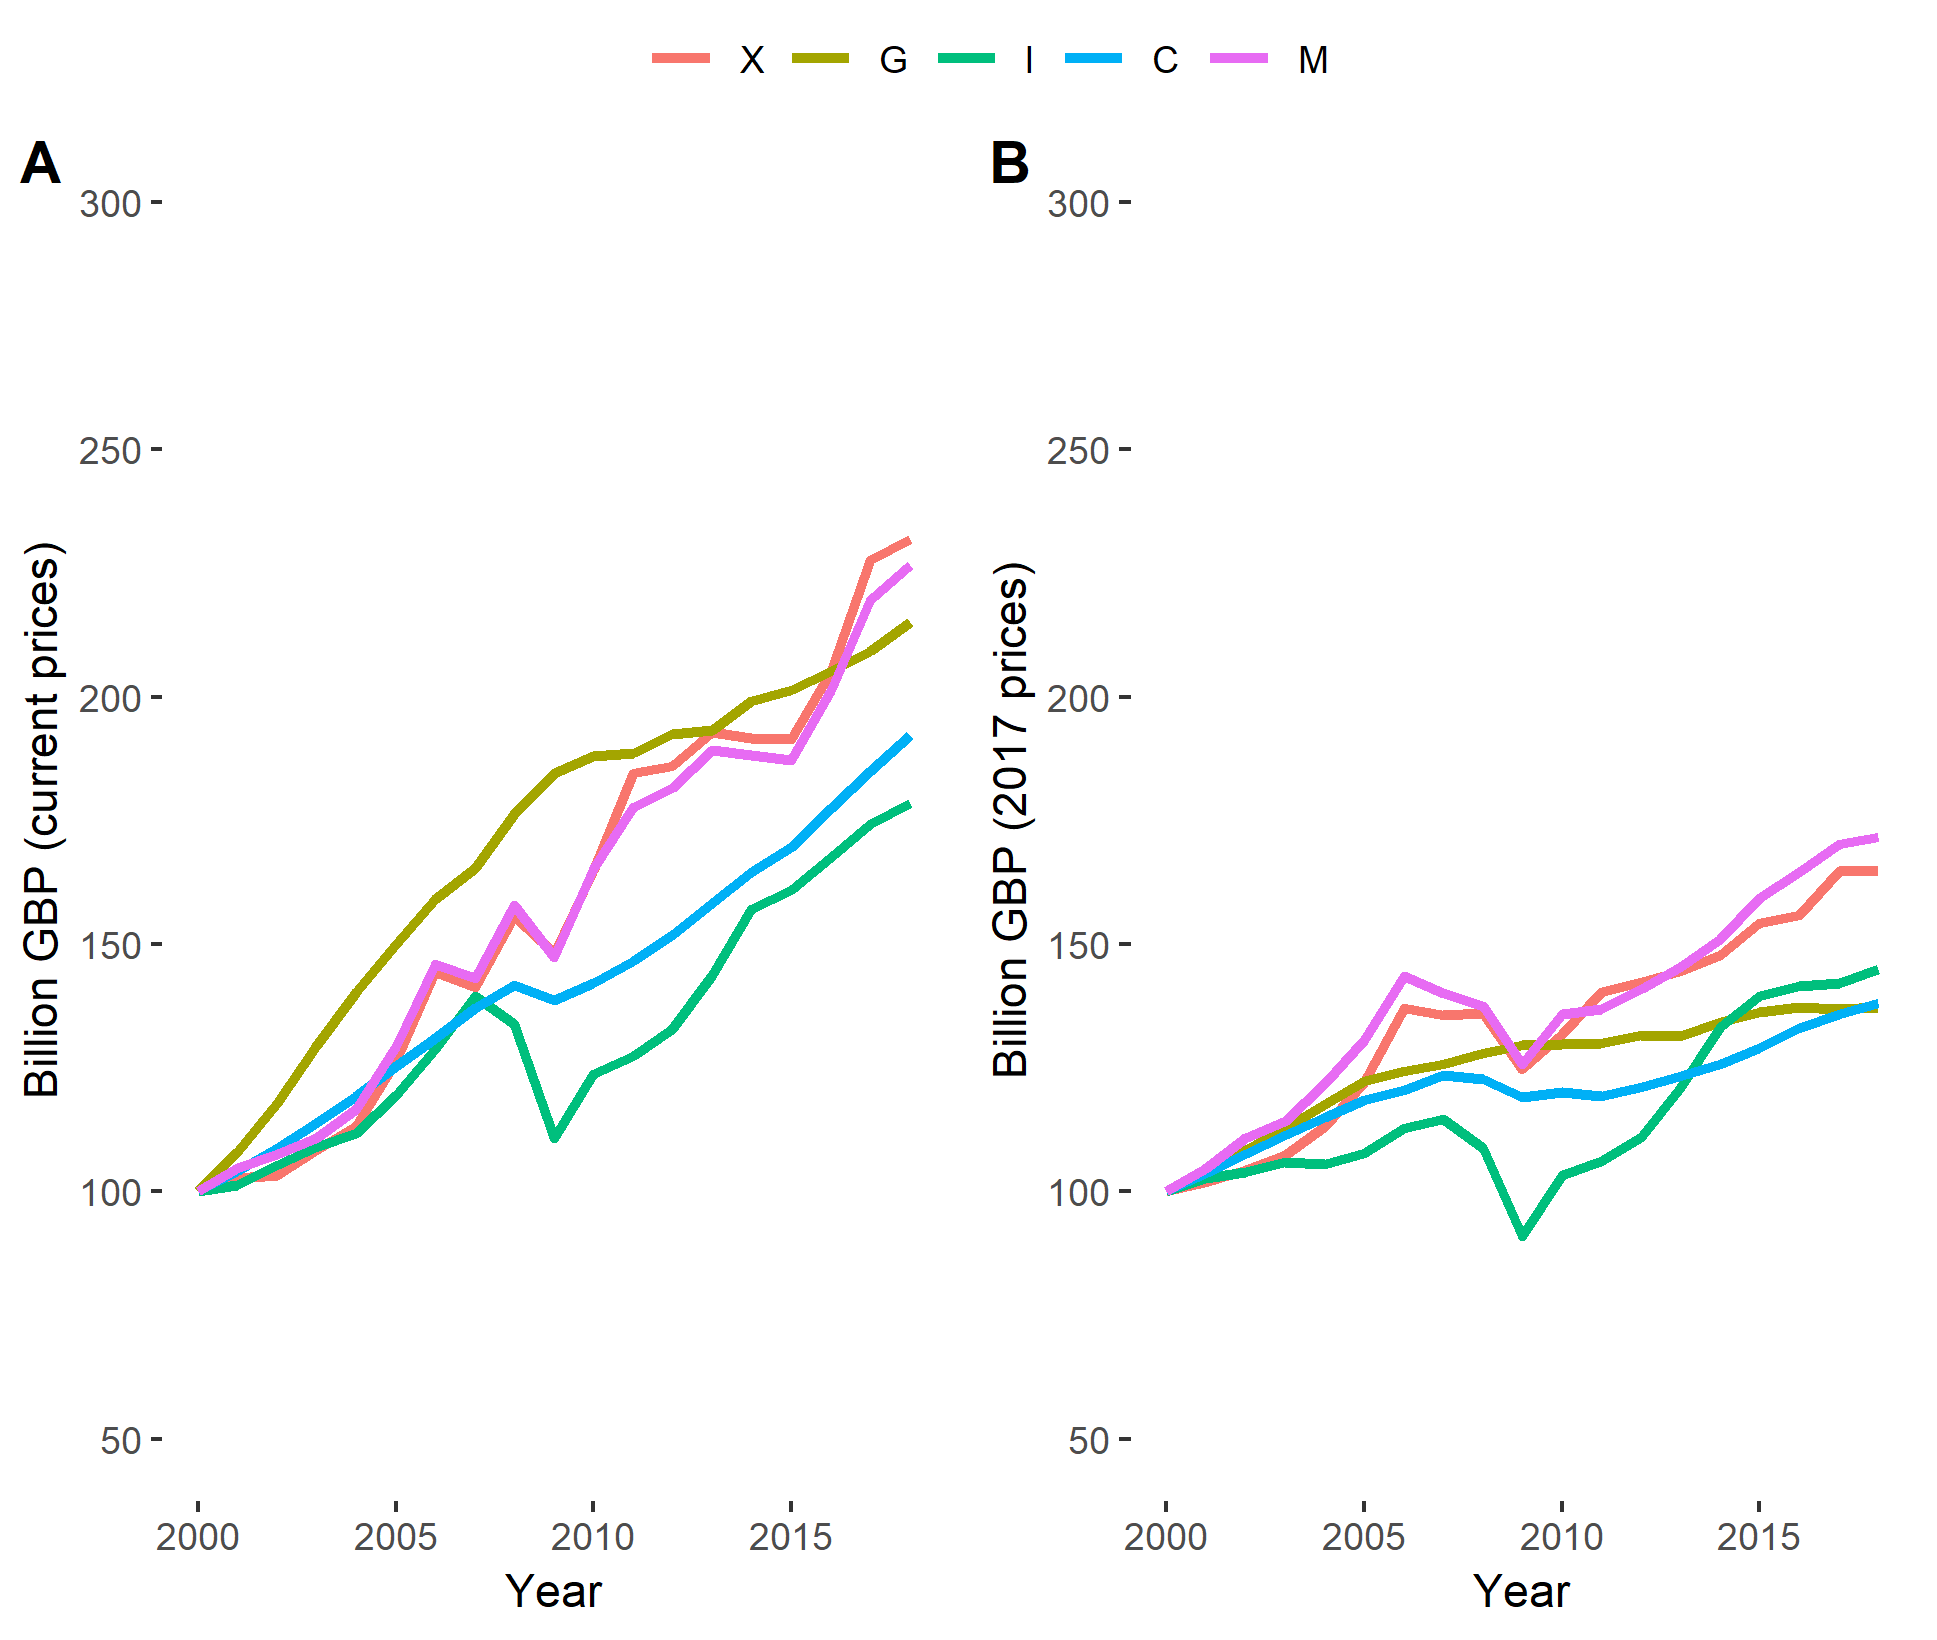
\includegraphics[width=0.8\linewidth]{_resources/chapter_gdp/fig3} 

}

\caption{The expenditure approach components of the Gross Domestic Product for the United Kingdom using line charts and an index with base year 2000. Data source: OECD. Values are converted to the 2017 price level using the GDP deflator for each category.}\label{fig:gdp5}
\end{figure}

\hypertarget{the-expendture-approach-and-economic-activity-in-microcountry}{%
\subsubsection{The expendture approach and economic activity in Microcountry}\label{the-expendture-approach-and-economic-activity-in-microcountry}}

Let us return to Microcountry and use the expenditure approach to calculate the economic activity of Microcountry.

\begin{itemize}
\tightlist
\item
  \(C\) household consumption:

  \begin{itemize}
  \tightlist
  \item
    The households buy bread at the bakery for 18£ and import goods from Neighbourcountry for 8£, \(C=8£+18£=26£\).
  \end{itemize}
\item
  \(G\) Government consumption:

  \begin{itemize}
  \tightlist
  \item
    The government spends 5£ on health services, \(G=5£\).
  \end{itemize}
\item
  \(I\) Investments:

  \begin{itemize}
  \tightlist
  \item
    There are no investments in this economy, \(I=0£\).
  \end{itemize}
\item
  \(X\) Exports:

  \begin{itemize}
  \tightlist
  \item
    The bakery exports bread to Neighbourcountry for 9£, \$X=9£.
  \end{itemize}
\item
  \(M\) Imports:

  \begin{itemize}
  \tightlist
  \item
    Microcountry imports goods for the value of 8£ from Neigbourcountry, \$M=8£.
  \end{itemize}

  The GDP of Microcountry is therefore \$Y=26£+5£+9£-8£=32£.
\end{itemize}

\hypertarget{the-income-approach}{%
\subsection{The income approach}\label{the-income-approach}}

A second approach to measuring GDP is the income approach. The income approach measures the GDP in terms of the generated income in the economy. The income generated in an economy consists of all compensation to workers (wages, pension contributions etc.), operating surplus (profits and rents) and sales taxes minus subsidies.\footnote{Note that while the notation for the expenditure approach is fairly standard, the notation for the production and income approaches are less standardized.}

\begin{align}
   \text{GDP}^{\text{I}} \text{=W+P+NT}
\end{align}
where

\begin{itemize}
\tightlist
\item
  \emph{W} is worker compensation.
\item
  \emph{P} is operating surplus.
\item
  \emph{NT} is sales taxes minus subsidies.
\end{itemize}

Sometimes you'll see that the income approach also incldues ``mixed income''. This term captures the value of work to the owners of self-employed firms. It is ``mixed'', because it is hard to tell whether it is profits or worker compensation. Figure \ref{fig:gdp6} shows the size of each of these three components for 2015 for the UK economy. Compensating of workers accounts for roughly half of the GDP, while operating surpluses account for about two-fifths. Note that the stacked area chart works better for the income approach compared to the expenditure approach, because all components are positive. The level of the top of the stacked area chart therefore corresponds to the actual GDP level.

\begin{figure}

{\centering 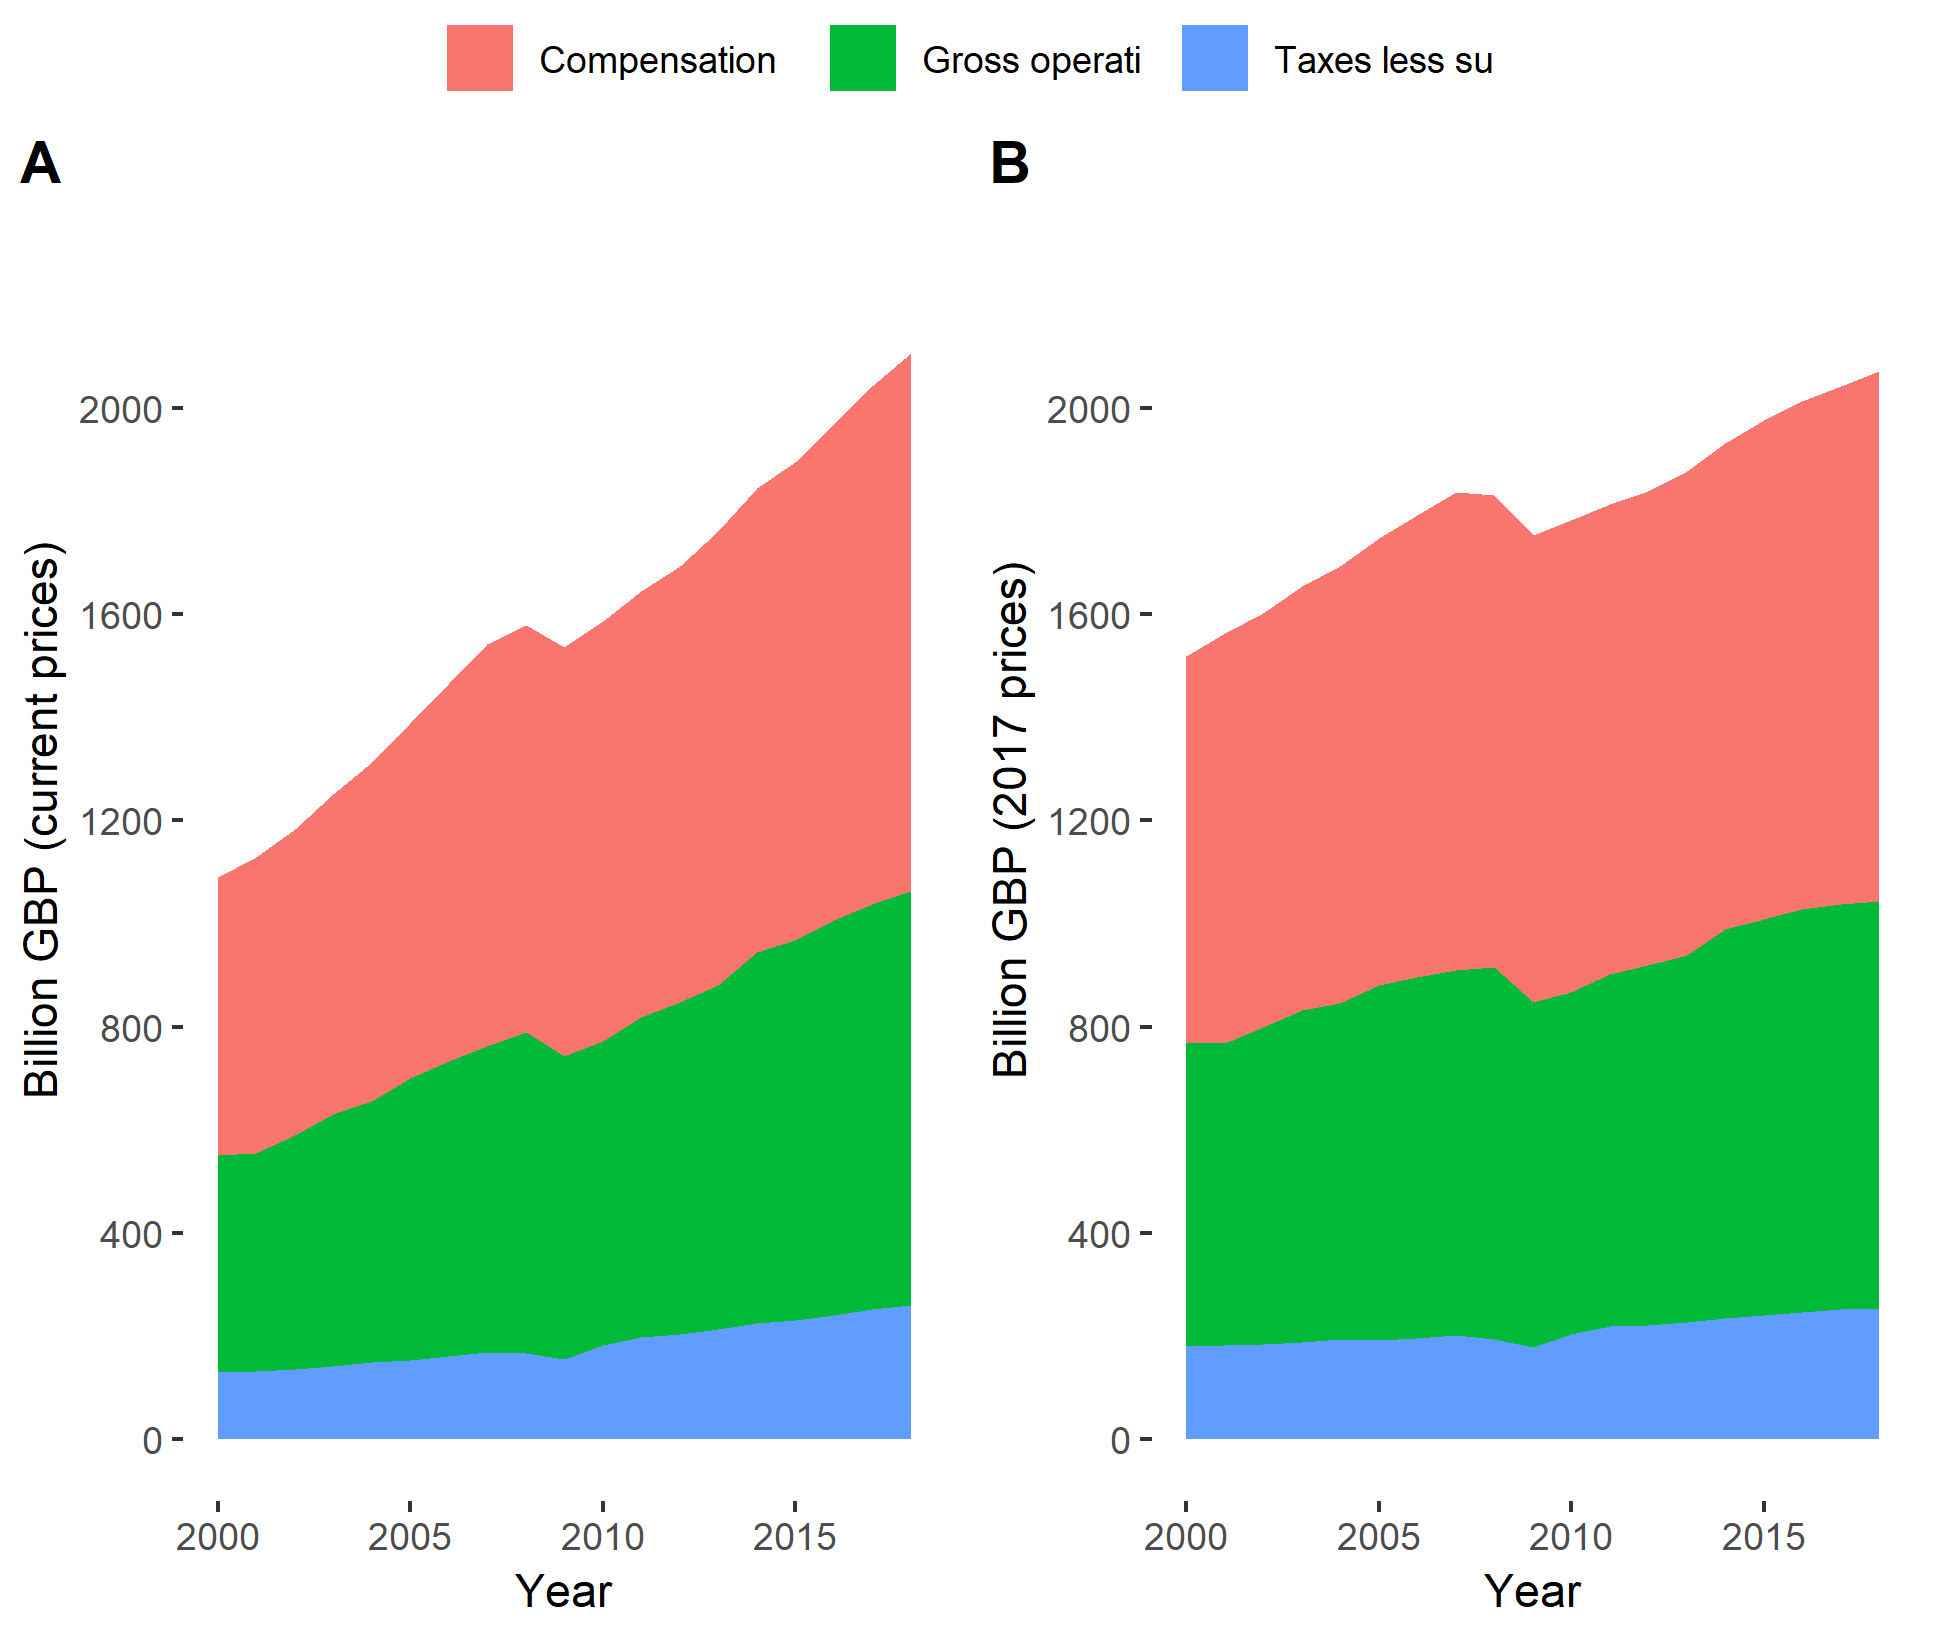
\includegraphics[width=0.9\linewidth]{_resources/chapter_gdp/fig4} 

}

\caption{The income approach components of the Gross Domestic Product for the United Kingdom using a stacked area chart. Data source: OECD. Values are converted to the 2017 price level using the overall GDP deflator.}\label{fig:gdp6}
\end{figure}

Figure \ref{fig:gdp7} shows the development of the wages (compensations of workers), profits (gross operation surplus) and taxes individually. The sharp decline in profits over the financial crisis is clearly visible. The growth in the wage component also flattened considerably over the financial crisis.

\begin{figure}

{\centering 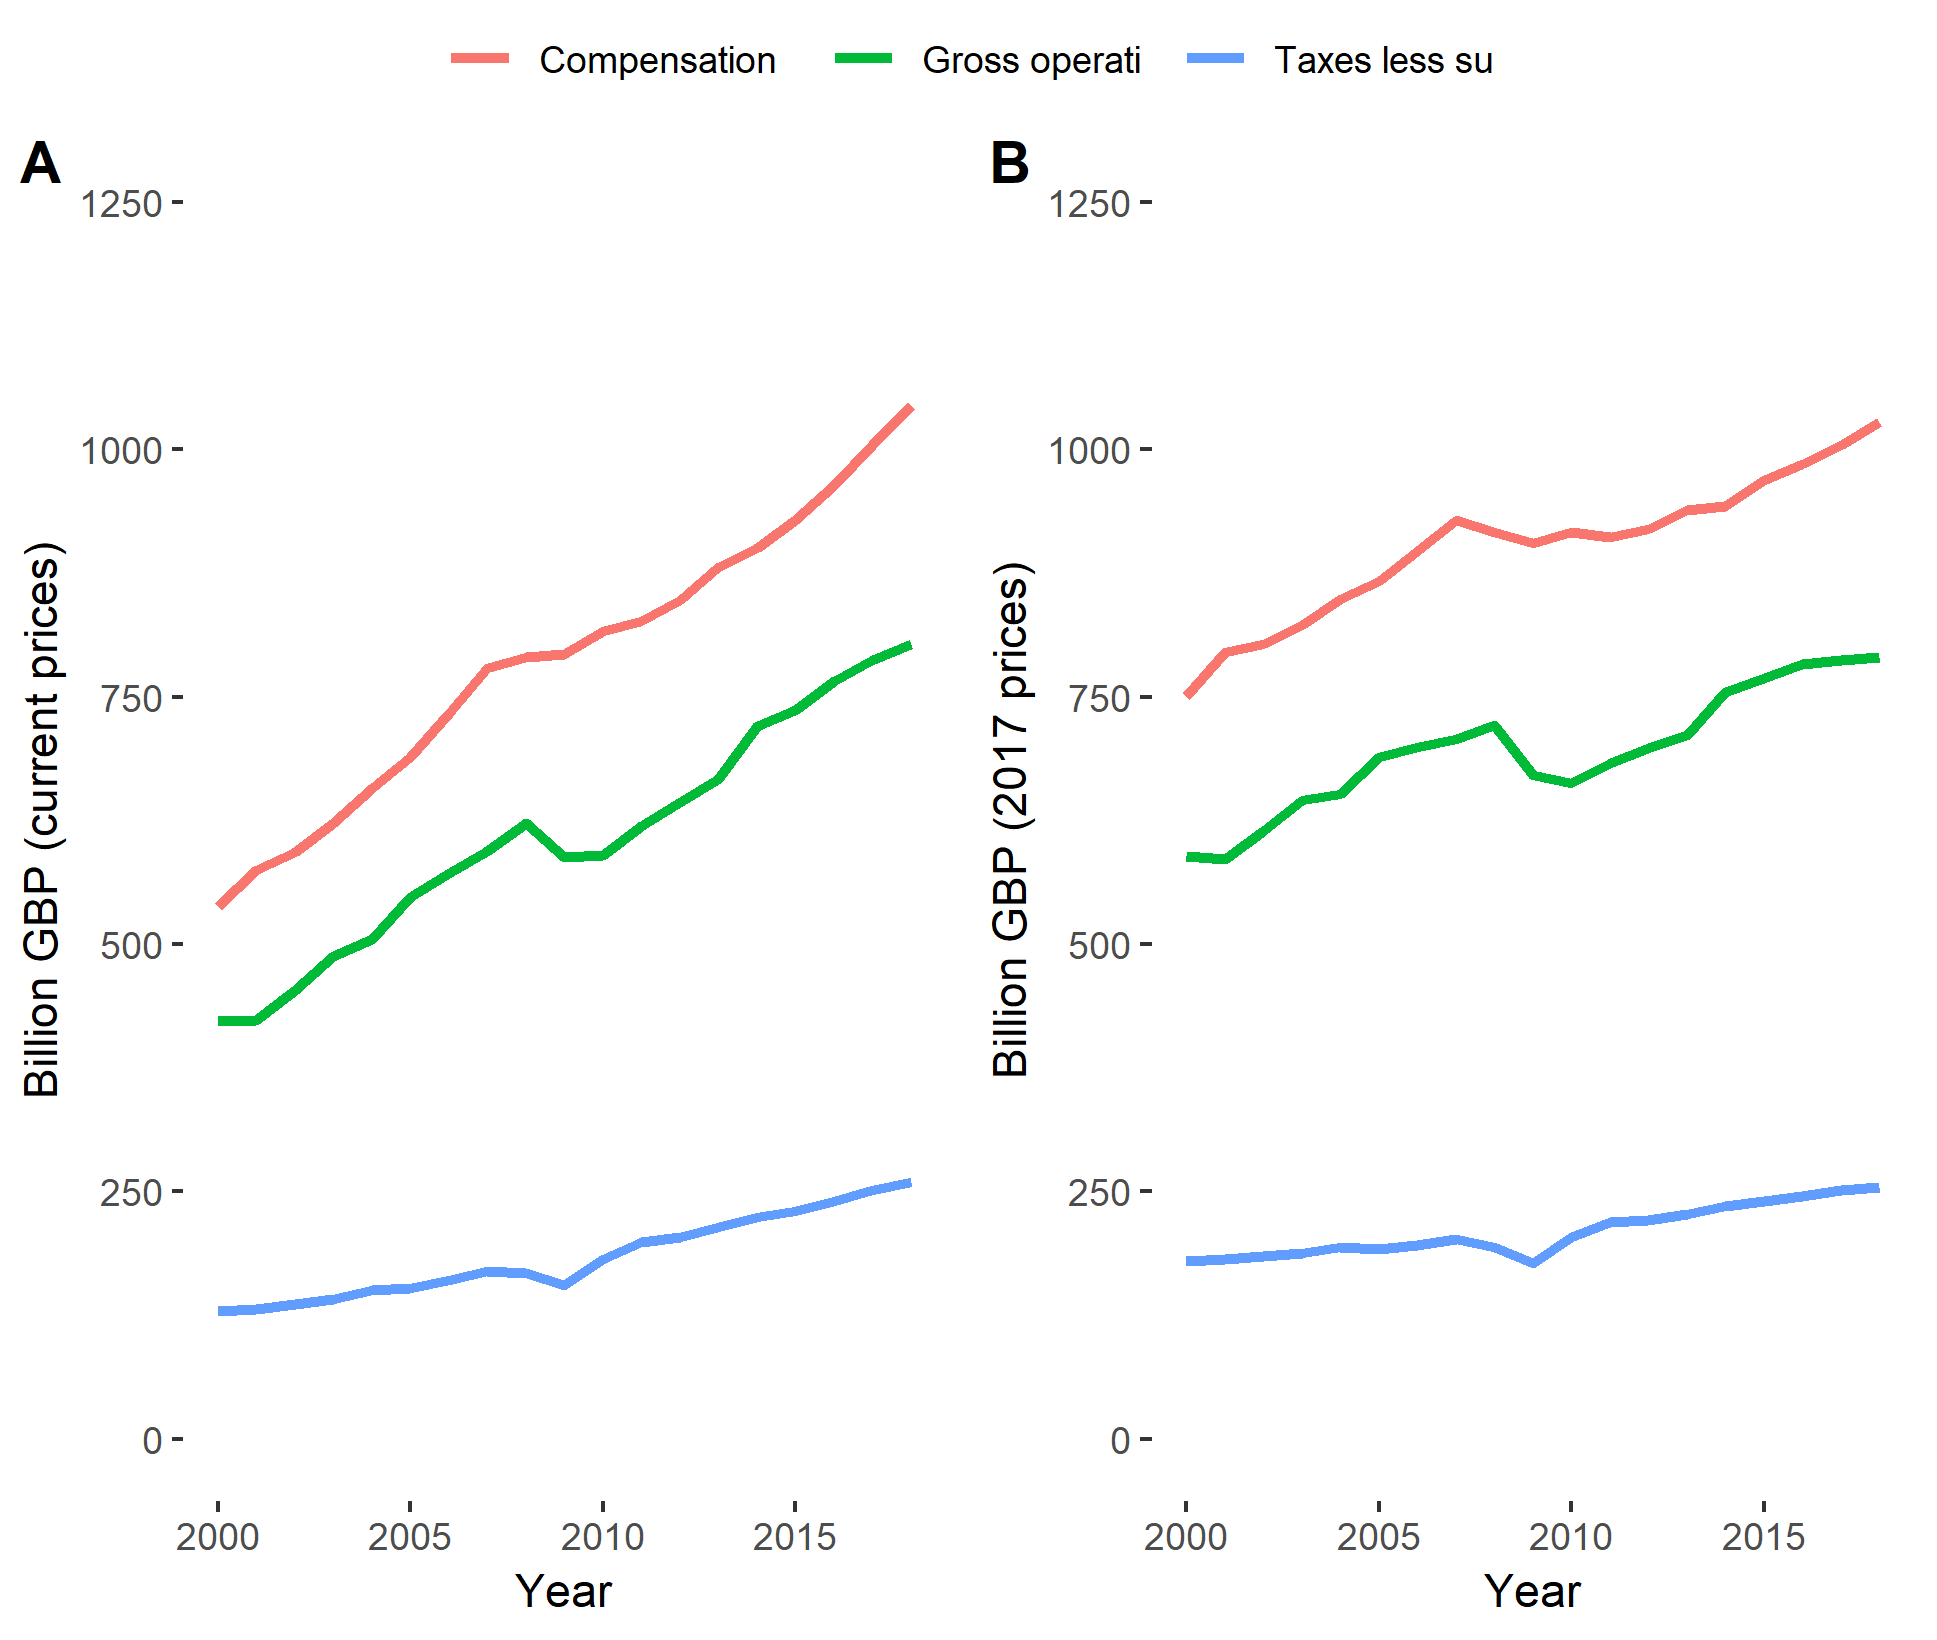
\includegraphics[width=0.9\linewidth]{_resources/chapter_gdp/fig5} 

}

\caption{The income approach components of the Gross Domestic Product for the United Kingdom using line charts. Data source: OECD. Values are converted to the 2017 price level using the overall GDP deflator}\label{fig:gdp7}
\end{figure}

Figure \ref{fig:gdp8} again illustrates the difference between real and nominal comparisons. In nominal terms, the incomes increased by between 80 and 100 percent. In real terms it was ``only'' about 30 to 40 percent. The sharp drop ion profits over the financial crisis is also clearly shown, but this category also increased sharply shortly after.

\begin{figure}

{\centering 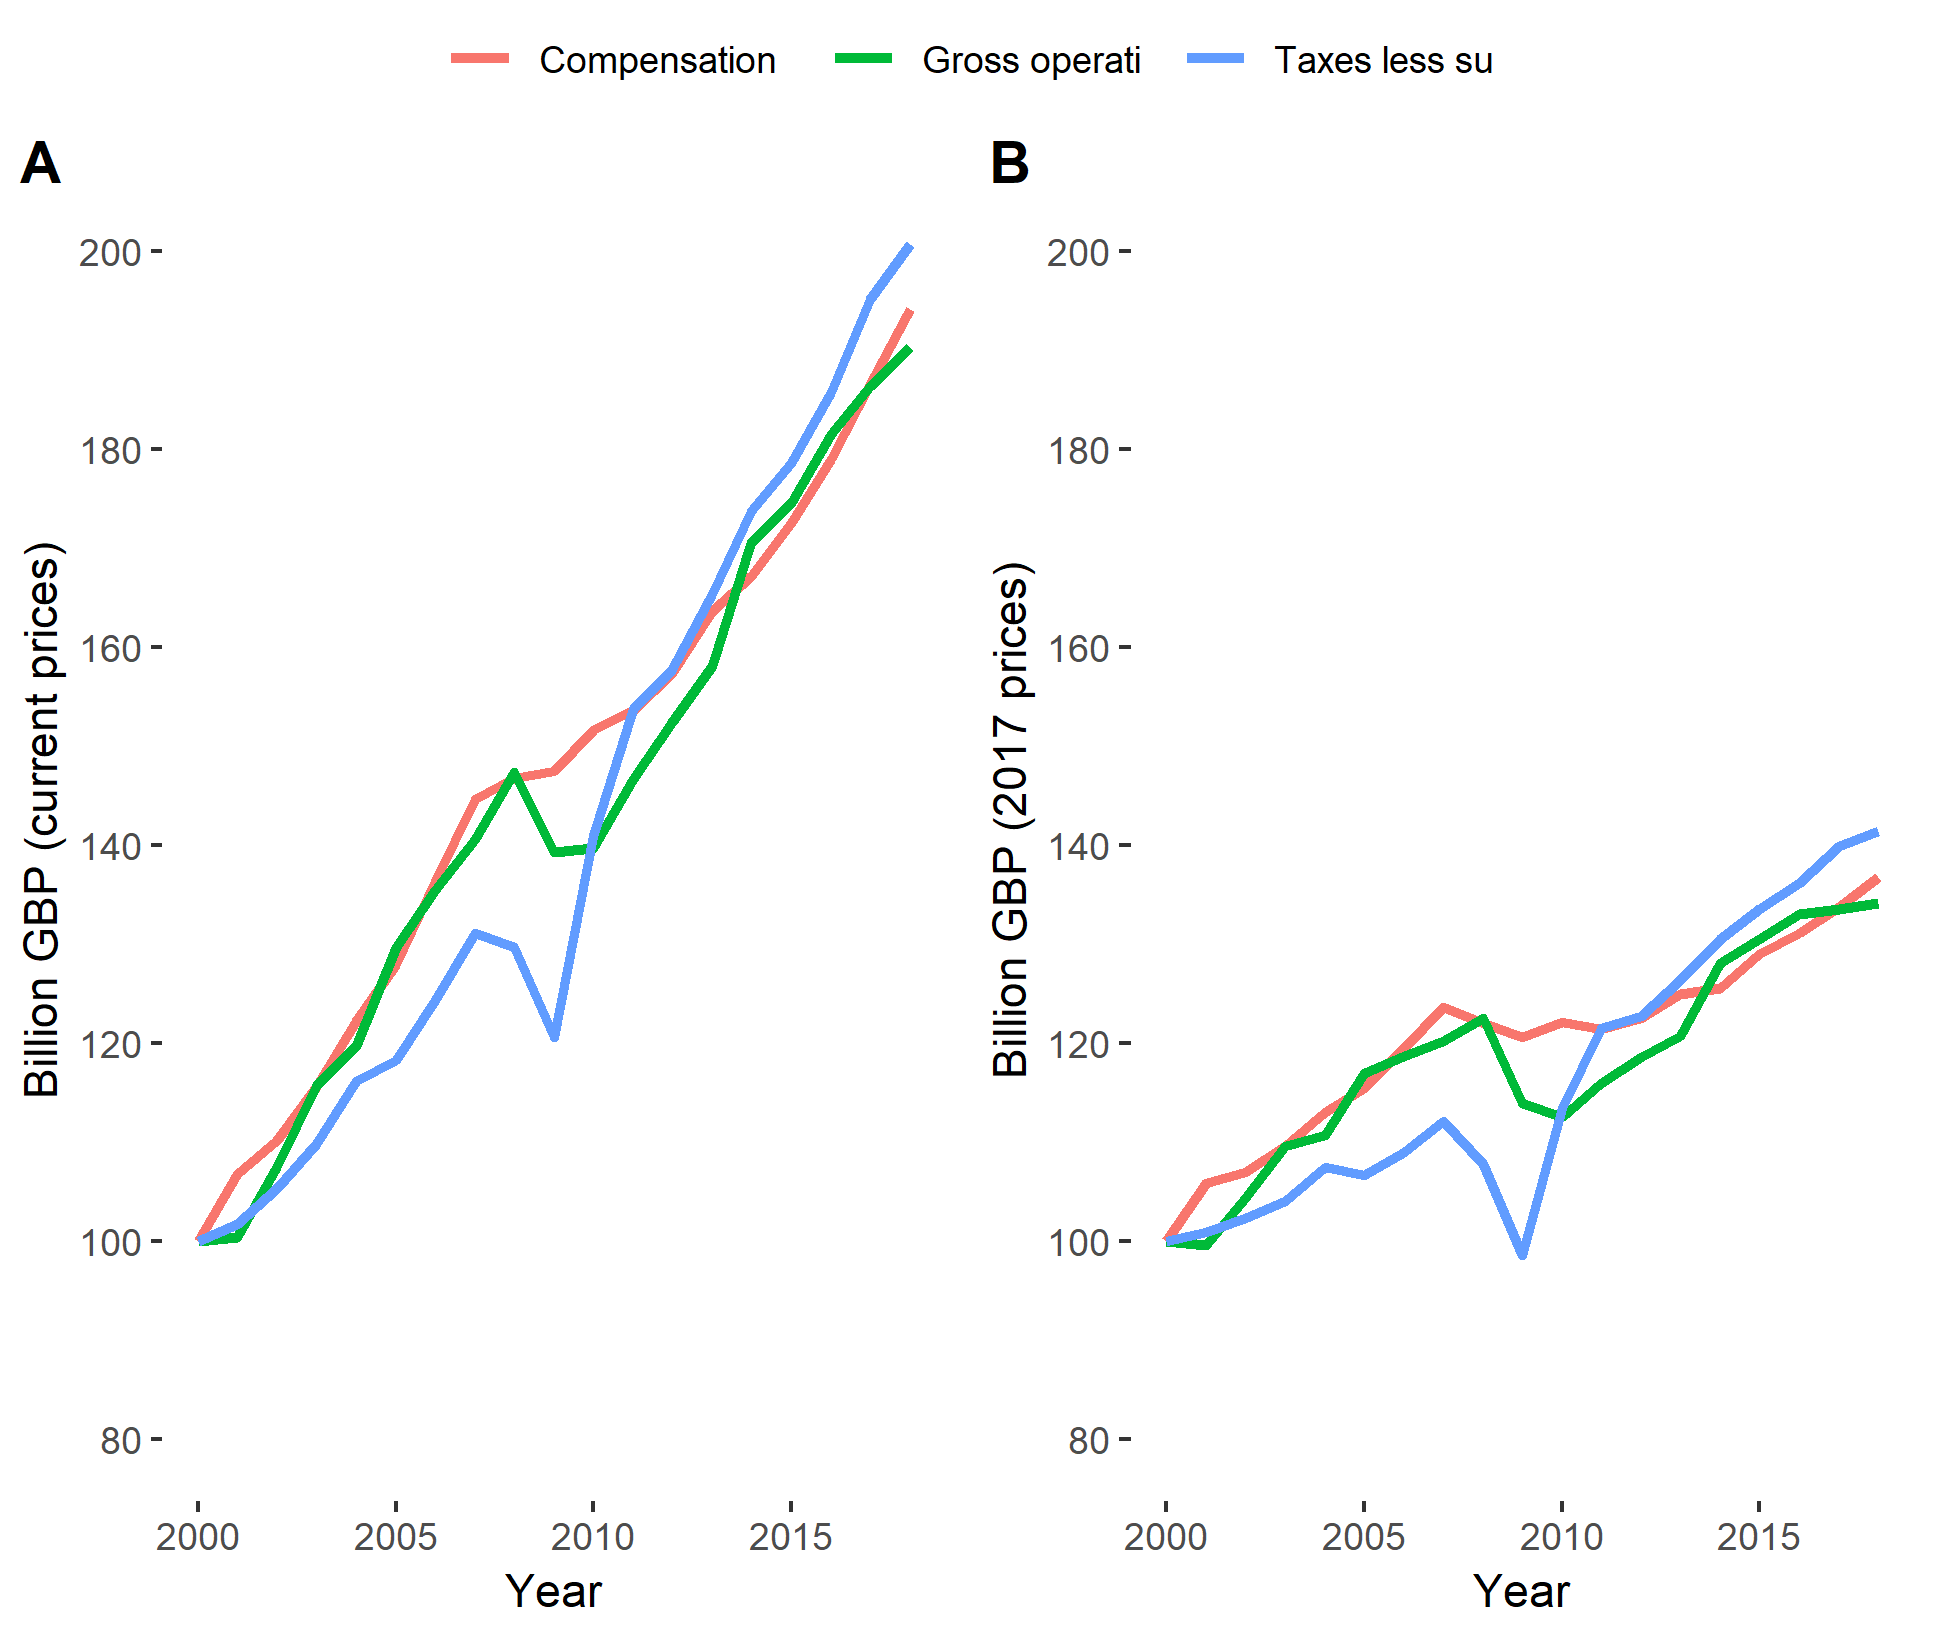
\includegraphics[width=0.9\linewidth]{_resources/chapter_gdp/fig6} 

}

\caption{The income approach components of the Gross Domestic Product for the United Kingdom using line charts and an index with base year 2000. Data source: OECD.  Values are converted to the 2017 price level using the overall GDP deflator.}\label{fig:gdp8}
\end{figure}

It is possible to decompose the income approach in further detail. We can investigate both wages and profits by sector to identify the sectors that contribute the most to GDP, and also to identify the sectors that were mostly affected by a recession. However, one challenge with the income approach is that these values are often not available in real terms. In Figures \ref{fig:gdp6} to \ref{fig:gdp8} we adjusted the current values to real values using the overall GDP. This is generally not recommended, because sub-categories might experience quite different price changes than overall GDP. In this case the deflator for each element of the income approach is not available.

\hypertarget{the-income-approach-and-economic-activity-in-microcountry}{%
\subsubsection{The income approach and economic activity in Microcountry}\label{the-income-approach-and-economic-activity-in-microcountry}}

Let us return to Microcountry and use the income approach to calculate the economic activity of Microcountry.

\begin{itemize}
\item
  \(W\),worker compensation:

  \begin{itemize}
  \tightlist
  \item
    The farm workers receive a wage compensation of 8£, the bakery workers receive a wage compensation of 14£ and the health service workers receive a compensation of 5£. The total wage comensation is therefore \(W=8£+14£+5£=27\).
  \end{itemize}
\item
  \(P\), operating surplus:

  \begin{itemize}
  \tightlist
  \item
    The farm has zero profits, but the bakery has a profit of 1£, \(P=1£\).
  \end{itemize}
\item
  \(NT\), taxes minus subsidies:

  \begin{itemize}
  \tightlist
  \item
    The farm pay 2£ in taxes and the bakery pays 2£. There are subsidies. The taxes minus subsidies is therefore, \(NT=2£+2£=4£\).
  \end{itemize}
\end{itemize}

The GDP of Microcountry is therefore \$Y=27£+4£+1£=32£.

\hypertarget{the-production-approach}{%
\subsection{The production approach}\label{the-production-approach}}

The third and last approach to measuring GDP is the production approach (also known as the output approach). So far we have considered how much we've spend (the expenditure approach), the income generated (the income approach) and now we finally look at how much we produce. The production approach measures the GDP in terms of production or \emph{value added}. The value added is the value of the output minus the costs of the intermediate goods. If a bakery buys flour for 15 £ and sells bread for 50 £, the value added by the bakery is 50-15=35 £. Intermediate goods are all goods used in the production process, such as raw materials, fuel, rental costs, cleaning and marketing costs.

We typically distinguish between two types of outputs, market and non-market outputs. The market output are goods and services sold on the market, such as the bread sold by the bakery. In that case the value added is straightforward to calculate, as it is the sales price minus the price of the intermediate goods. However, not not all goods are necessarily sold, so we also include the change in inventories. For non-market output, such as health and defense, the output is the production costs, i.e.~the cost of labor and intermediate goods (and depreciation in fixed assets). Finally, there is a distinction between value added in basic prices and value added in market prices. To obtain the latter we have to add sales tax and subtract subsidies.

\begin{align}
   \text{GDP}^{\text{P}} \text{=GVA+NT}
\end{align}
where

\begin{itemize}
\tightlist
\item
  \emph{GVA} gross value added.
\item
  \emph{NT} is taxes minus subsidies.
\end{itemize}

It should be noted that NT in this case not necessarily equals NT in the income approach. This is because taxes and subsidies here only relate to the taxes and subsidies on goods produced domestically. In the income approach taxes and subsidies refer to the products produced domestically and the products that are imported. Figure \ref{fig:gdp9} the development of these components by sectors of the UK economy. As all aspects contribute positively to the overall GDP, we can interpret the height of the stacked area chart as the overall GDP level.\footnote{Note that this would not be the case if subsidies were larger than taxes.}

\begin{figure}

{\centering 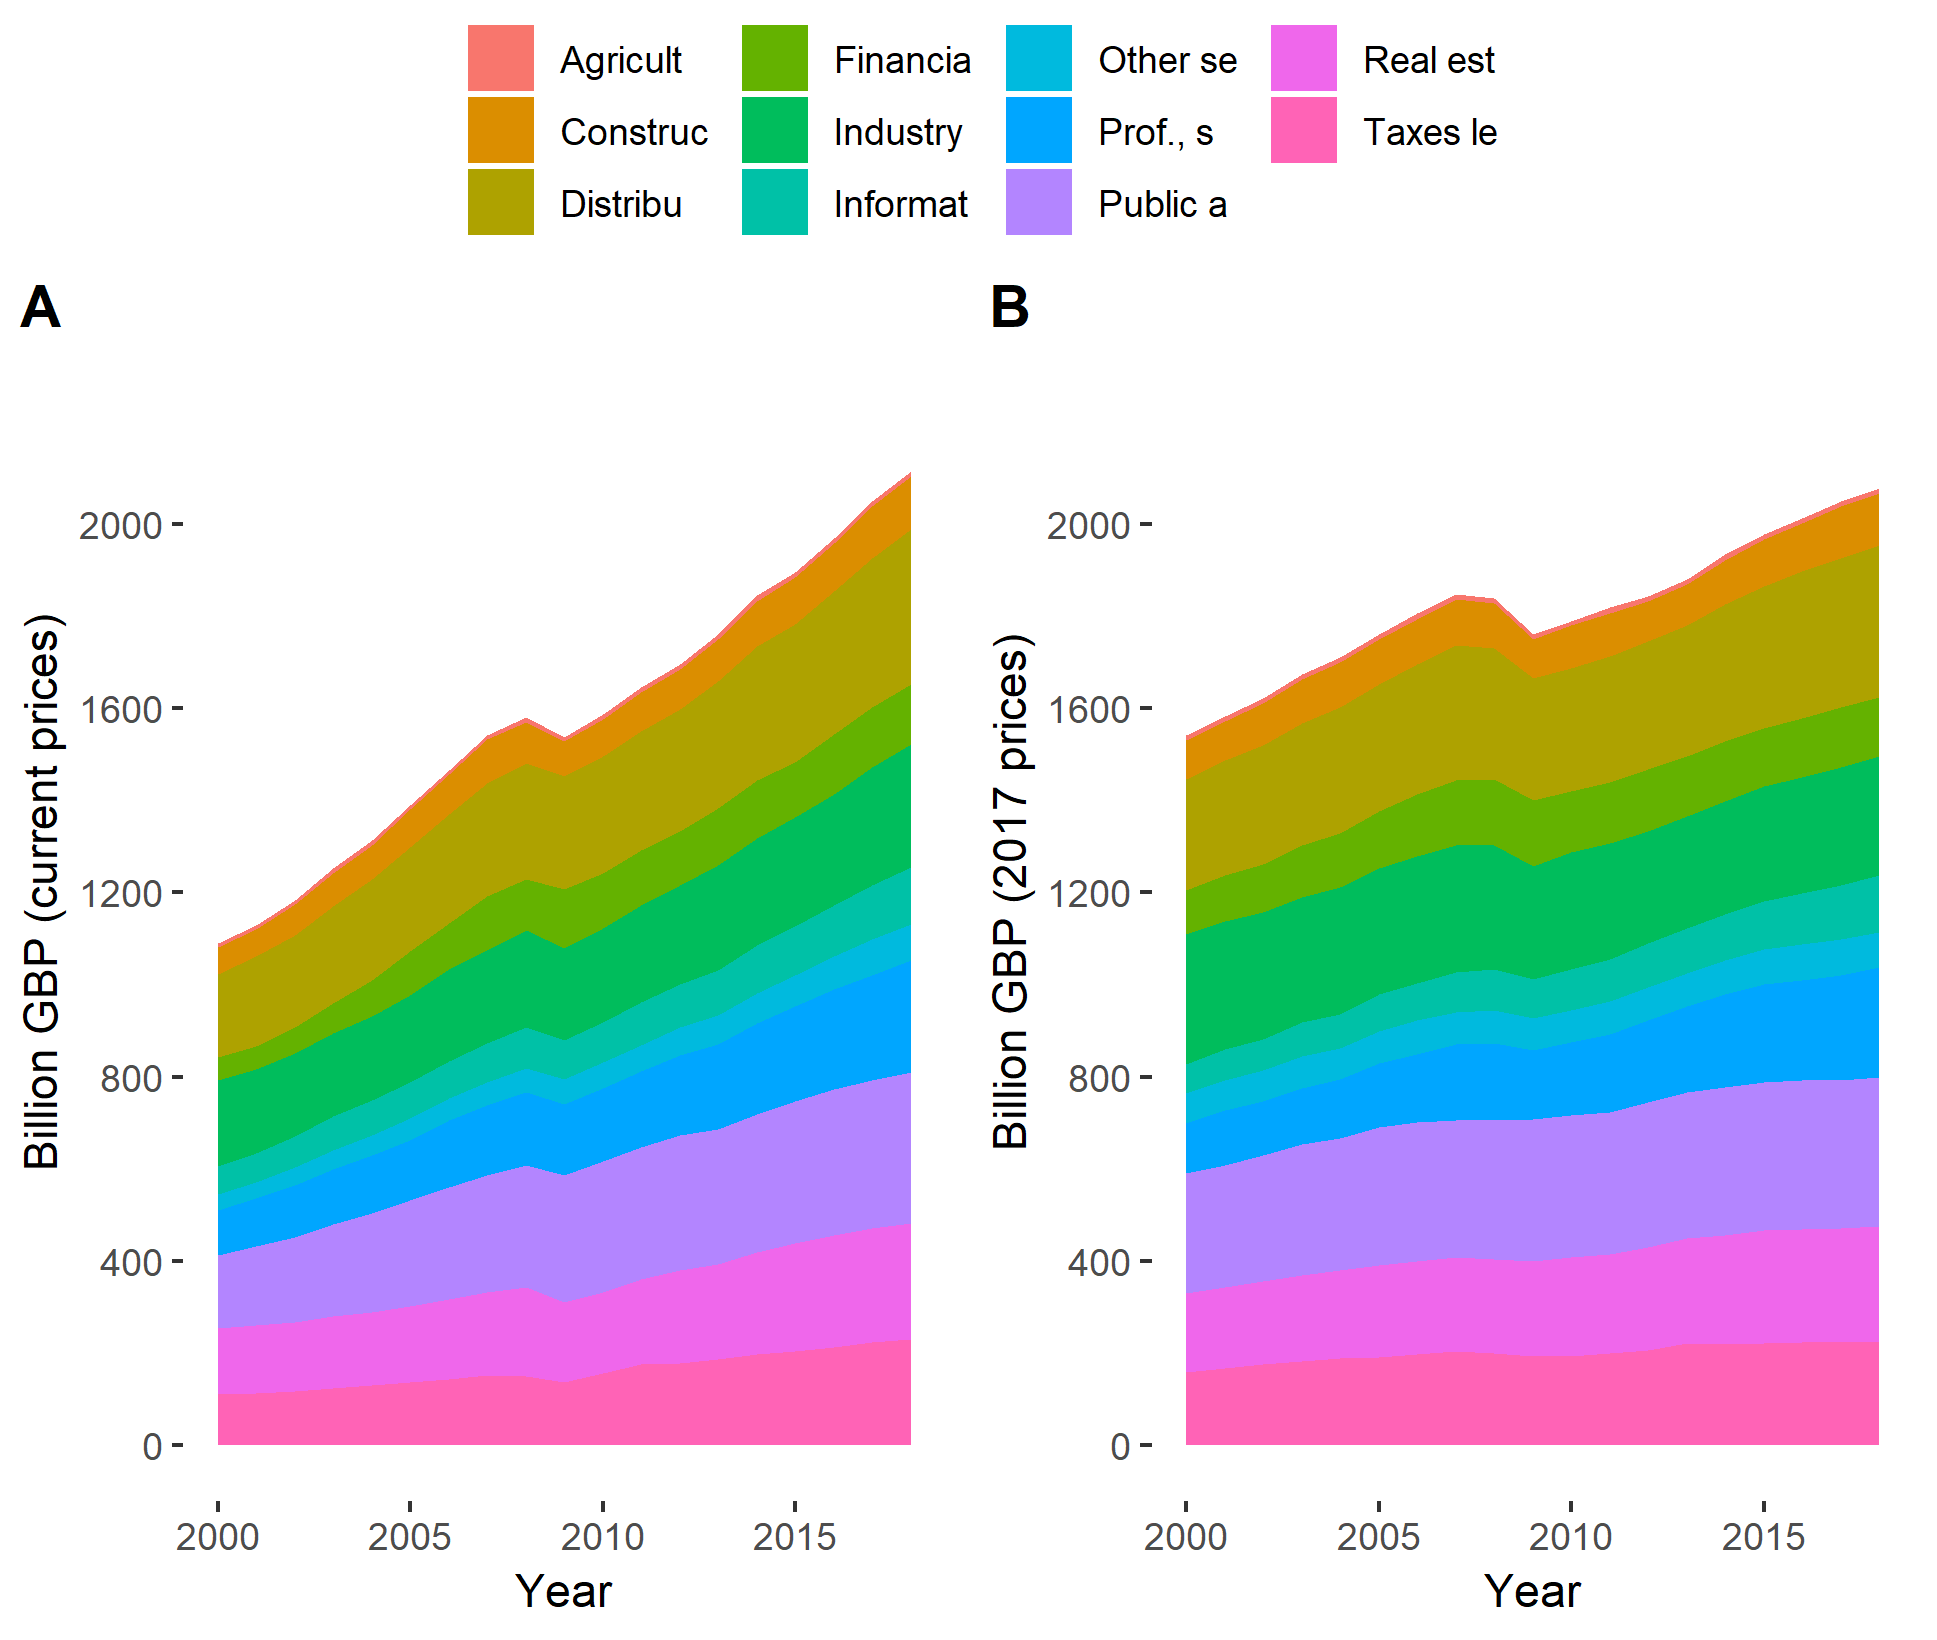
\includegraphics[width=0.9\linewidth]{_resources/chapter_gdp/fig7} 

}

\caption{The production approach components of the Gross Domestic Product for the United Kingdom using a stacked area chart. Data source: OECD. Values are converted to the 2017 price level using the GDP deflator for each category.}\label{fig:gdp9}
\end{figure}

The stacked area chart is appealing, but it is hard to get a sense of the individual values. Again, the line chart (shown in Figure \ref{fig:gdp10}) is a lot more informative about the individual levels.

\begin{figure}

{\centering 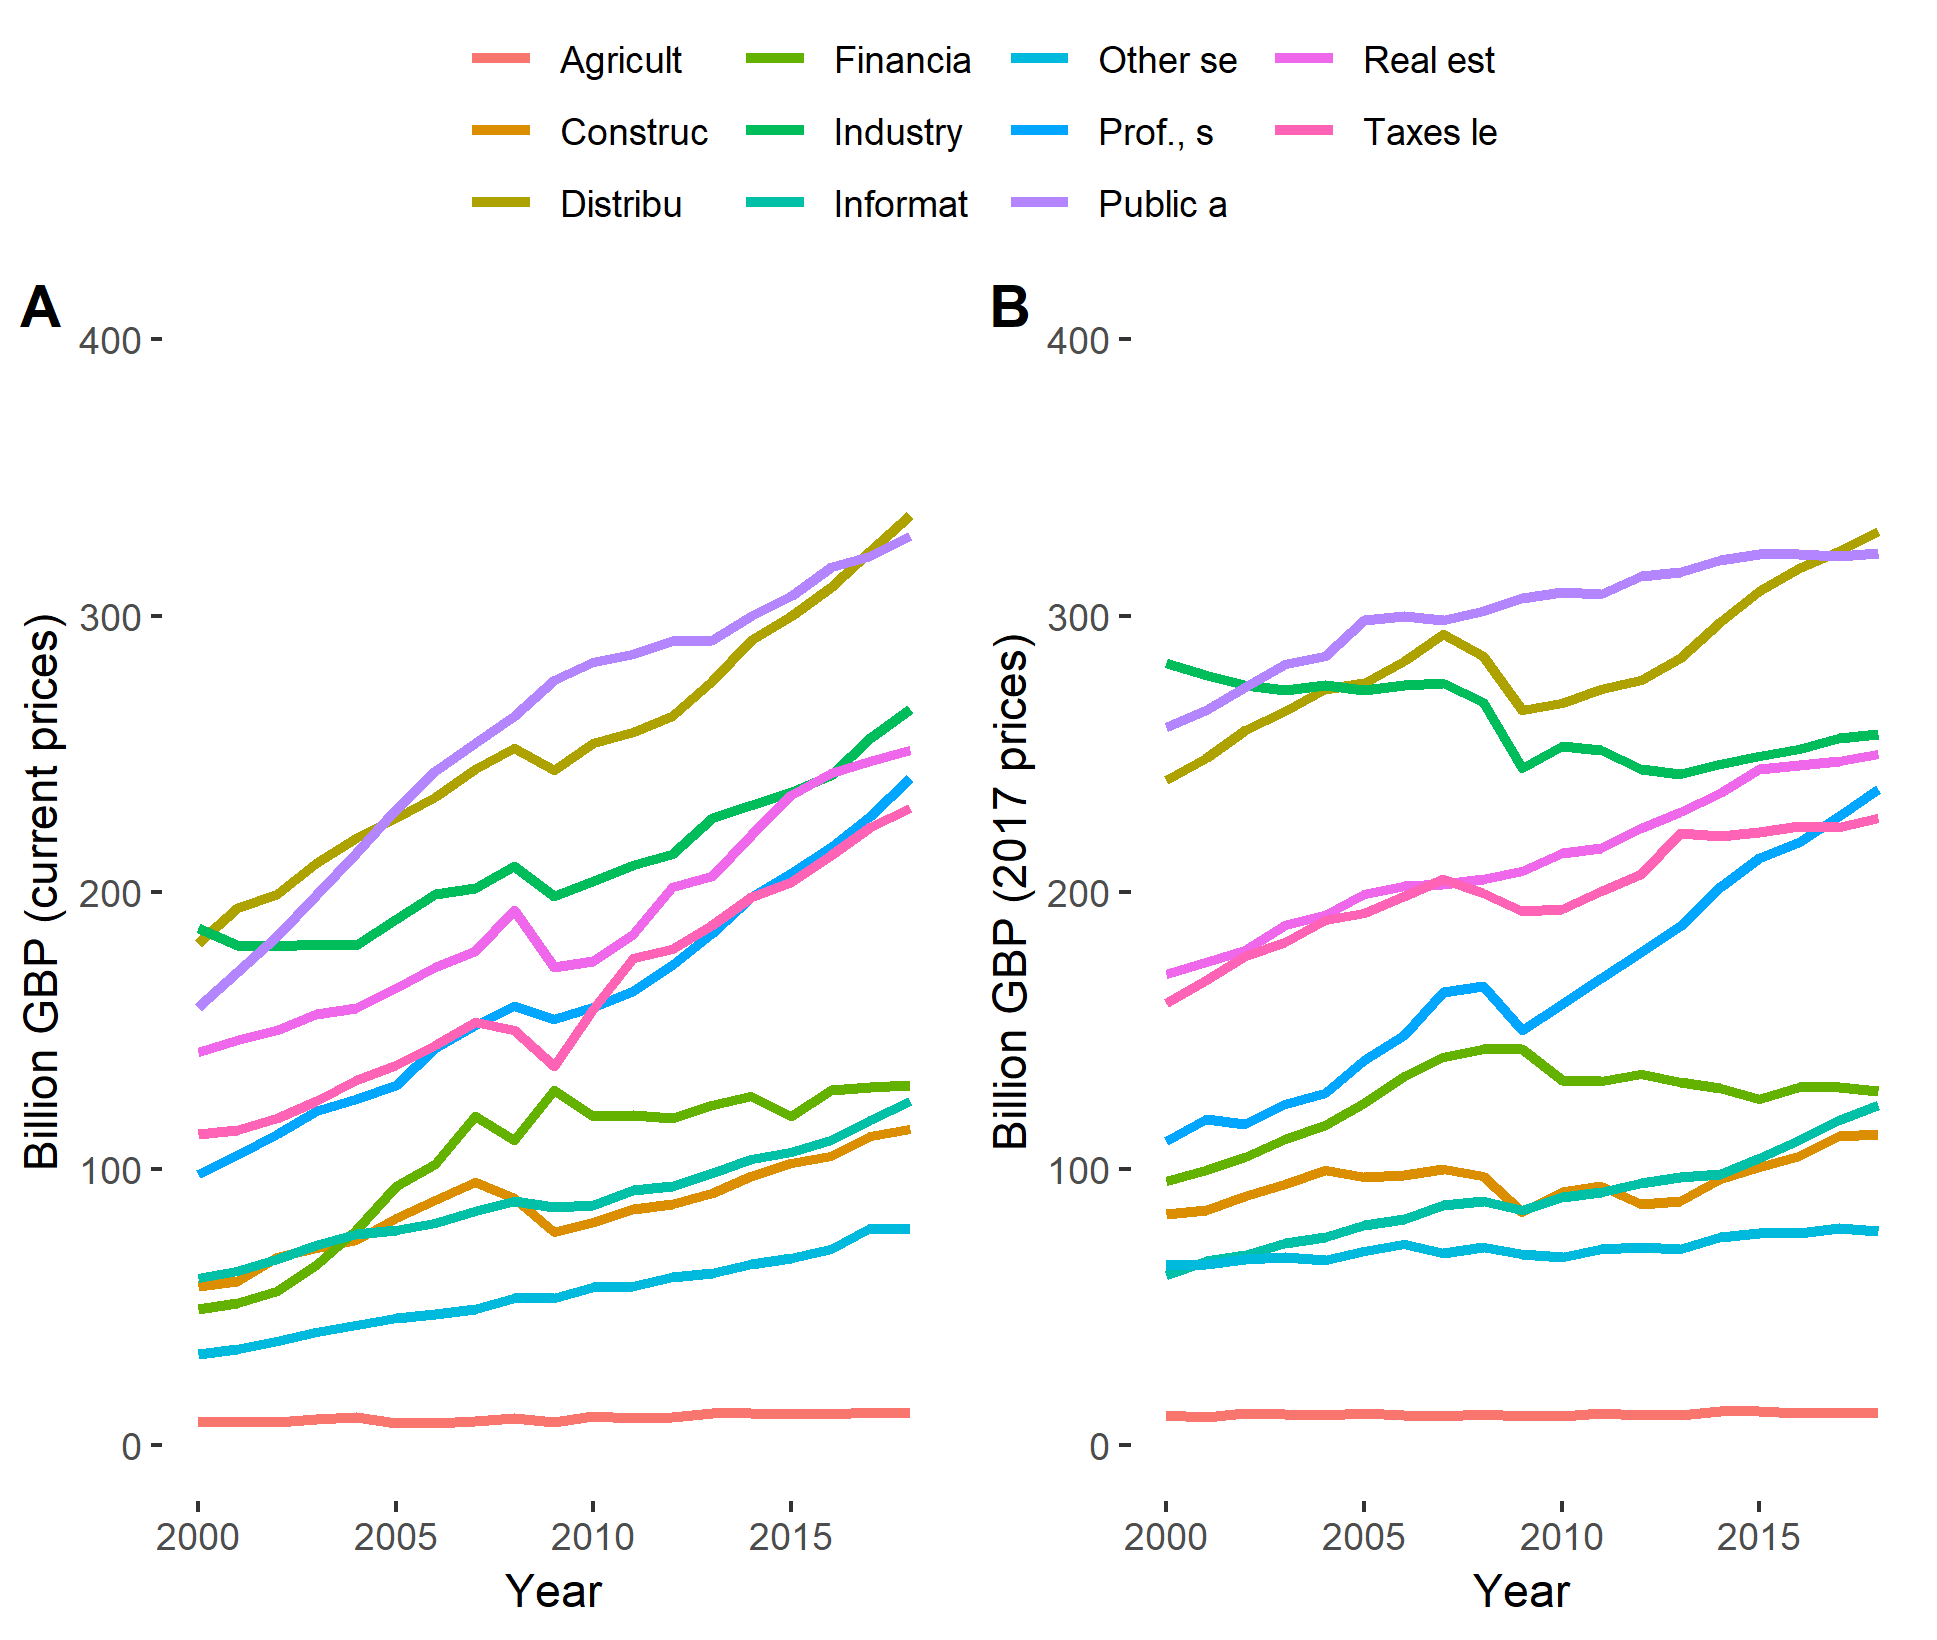
\includegraphics[width=0.9\linewidth]{_resources/chapter_gdp/fig8} 

}

\caption{The production approach components of the Gross Domestic Product for the United Kingdom using line charts. Data source: OECD. Values are converted to the 2017 price level using the GDP deflator for each category.}\label{fig:gdp10}
\end{figure}

The index line chart in Figure \ref{fig:gdp11} shows that some sectors are still below their 2000 level in real value added terms (for example the sector ``Industry, including energy'').

\begin{figure}

{\centering 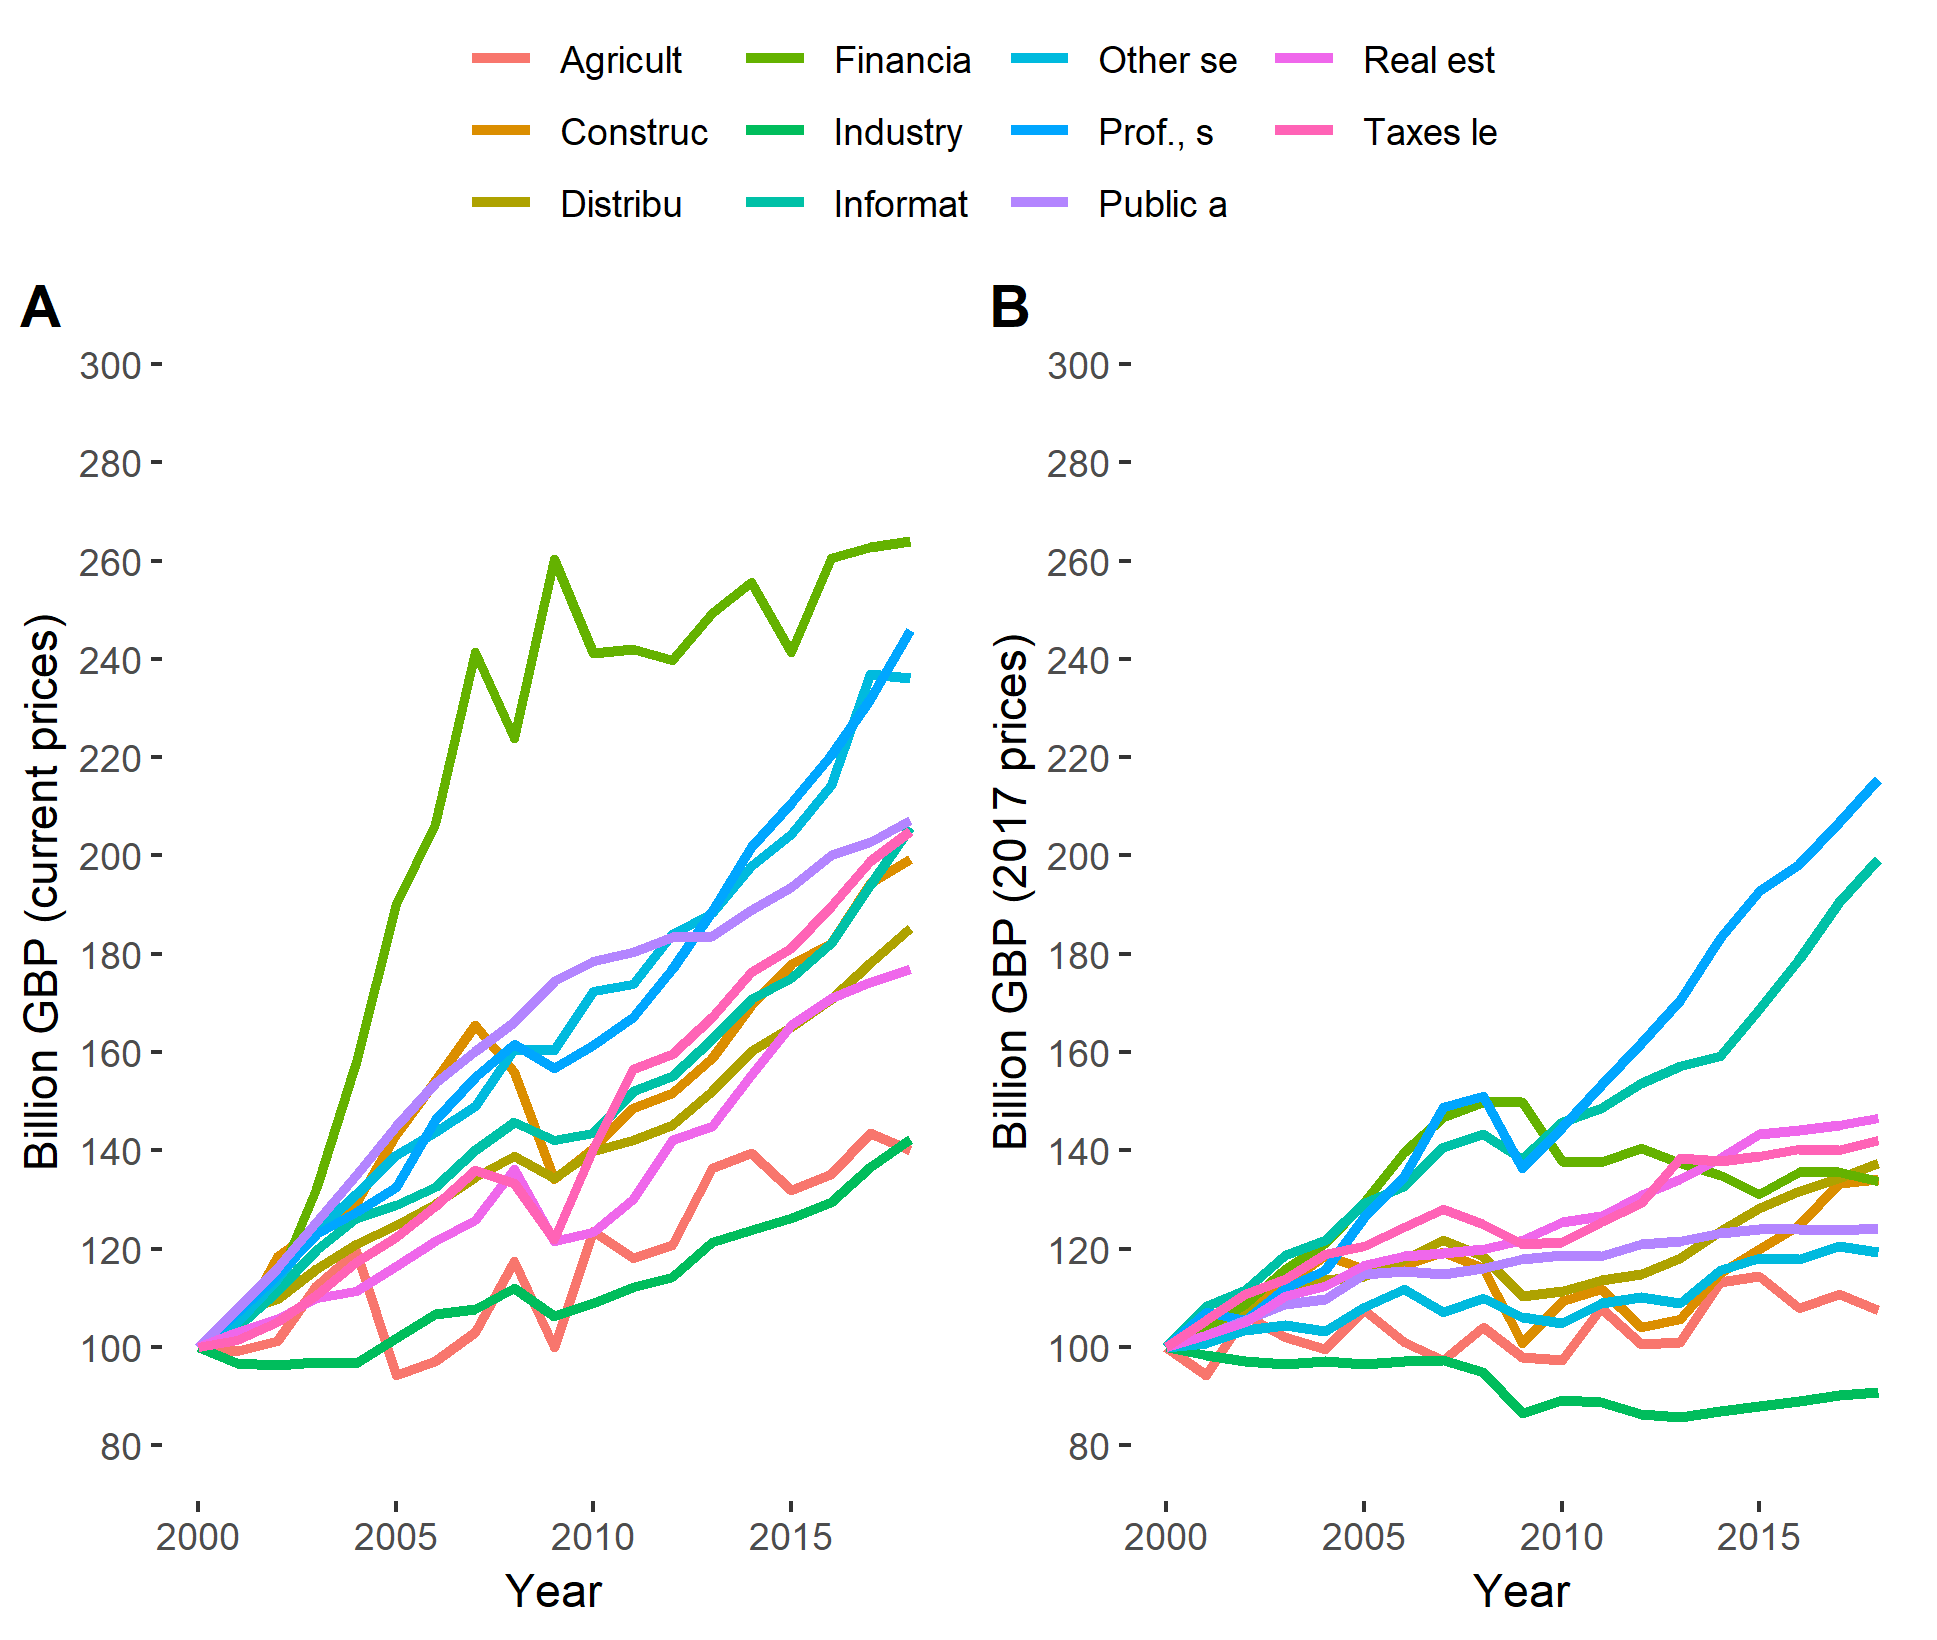
\includegraphics[width=0.9\linewidth]{_resources/chapter_gdp/fig9} 

}

\caption{The production approach components of the Gross Domestic Product for the United Kingdom using line charts and an index with base year 2000. Data source: OECD. Values are converted to the 2017 price level using the GDP deflator for each category}\label{fig:gdp11}
\end{figure}

\hypertarget{the-production-approach-and-economic-activity-in-microcountry}{%
\subsubsection{The production approach and economic activity in Microcountry}\label{the-production-approach-and-economic-activity-in-microcountry}}

Let us return to Microcountry and use the expenditure approach to calculate the economic activity of Microcountry.

\begin{itemize}
\item
  \(GVA\), gross value added

  \begin{itemize}
  \item
    The farm sells flour for 10£ and pays 2£ in taxes. The gross value added of the bakery is therefore 8£. The bakery sells bread for 27£, pays a sales tax of 2£ and pays 10£ for the flour from the bakery. The gross value added of the bakery is therefore 15£. Finally, the public sector provides a health service. The value of public sector provision is typically estimated by means of the costs, which in this case is 5£. The total gross value added in Microcountry is therefore \$GVA=8£+15£+5£=28£.
  \item
    The farm pay 2£ in taxes and the bakery pays 2£. There are subsidies. The sales taxes minus subsidies is therefore, \(NT=2£+2£=4£\).
  \end{itemize}
\end{itemize}

The GDP of Microcountry is therefore \(Y=28\)+4£=32£.

\hypertarget{what-is-included-in-the-gdp-measure}{%
\subsection{What is included in the GDP measure?}\label{what-is-included-in-the-gdp-measure}}

Measuring GDP also requires us to understand which activities we should include, and which we should not include. Based on the general principles described in the \citep{esa2010}, the Office for National Statistics decides on an production boundary, which contains all economic activities that should be included in the GDP measurements. An activity is included in the boundaries if:

\begin{itemize}
\tightlist
\item
  The activity produces a meaningful output.
\item
  The product or activity has a meaningful market value, or the market value can be imputed.
\item
  The inclusion of the activity increases the meaningfulness of cross-country comparisons.
\end{itemize}

Several activities are less clear-cut that you might think, for example activities where ``production is forbidden by law; as long as all units involved in the transaction enter into it voluntarily'' are included. Breeding of fish in fish farms is included, but breeding of fish in open seas is not included.

\hypertarget{gdp---why-3-approaches}{%
\subsection{GDP - Why 3 approaches?}\label{gdp---why-3-approaches}}

Note how all three approaches shown result in the same GDP. For simplicity, one might therefore argue that we should just stick to one approach and ignore the two other approaches. However, each approach has its own advantage. First, expenditure approach is very useful if you want to assess whether changes in GDP are driven by for example domestic consumption or exports. Moreover, we can decompose all approaches in more detail. We could for example identify which sector is contributing most to the value added using the production approach.

As noted, the three approaches to measuring GDP should all lead to the same overall GDP. As an illustration, Table \ref{fig:gdp12} shows the GDP components for each of the three approaches for the United Kingdom in 2017. While the three approaches in theory should lead to exactly the same number, we often observe small discrepancies in practice. These discrepancies are called ``statistical discrepancy'' and area as Table \ref{fig:gdp12} shows relatively small. The table also illustrates why the three approaches are useful: they are informative about different perspectives. We could ask, was the recession mainly related to a drop in private consumption or exports (based on the expenditure approach)? Or, was the recession mainly related to a drop in profits or compensation of employees (the income approach). Or, which sector's production dropped most during the recession?

\begin{figure}

{\centering 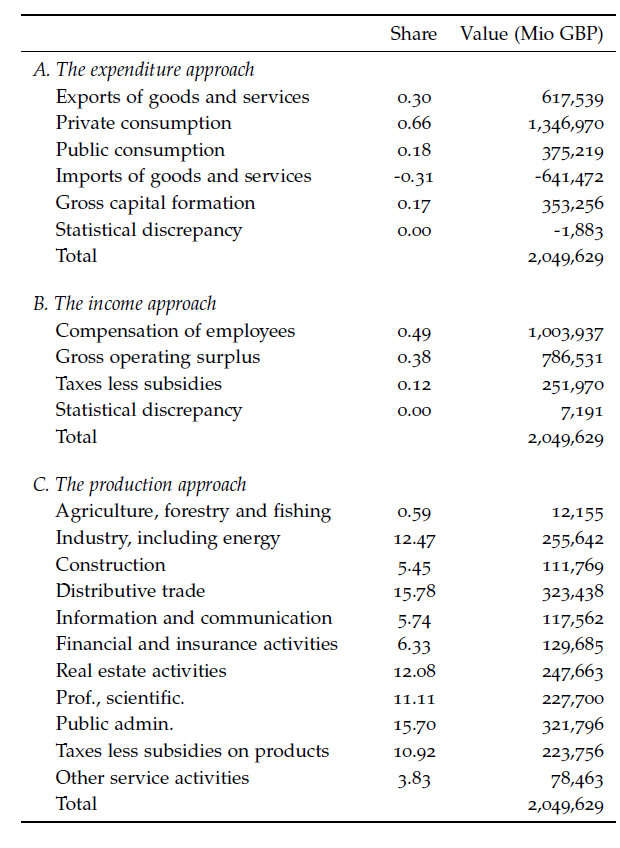
\includegraphics[width=0.8\linewidth]{_resources/chapter_gdp/tab1} 

}

\caption{Gross Domestic Product of the United Kingdom in 2017.Data source: OECD. All values are in 2017 prices.}\label{fig:gdp12}
\end{figure}

\begin{myblock}
\textbf{Measuring GDP - an overview}

\emph{1. The expenditure approach}

\begin{itemize}
\tightlist
\item
  The expenditure approach (called the spending approach in {[}@core{]})
  measures the GDP in terms of expenditures by households and the
  Government, as well investments and net exports of goods and services
  (i.e.~exports minus imports).
\end{itemize}

\begin{align}
  Y=C+G+I+X-M=C+G+I+NX
\end{align}

\begin{itemize}
\tightlist
\item
  \emph{Y} is the Gross Domestic Product (GDP).
\item
  \emph{C} is final consumption of goods and services by households. It
  includes goods like food, cars, and clothing, as well as services such
  as hotel stays.
\item
  \emph{G} is final consumption expenditure of goods and services by the
  government.
\item
  \emph{I} is investments (also called gross capital formation) are
  investments in fixed assets such as machinery, buildings etc.
\item
  \emph{X} is goods and services produced domestically but consumed
  abroad (Exports)
\item
  \emph{M} is goods and services produced abroad and consumed
  domestically (Imports).
\end{itemize}

\emph{2. The income approach}

\begin{itemize}
\tightlist
\item
  The income approach measures the GDP in terms of the generated income
  in the economy.
\end{itemize}

\begin{align}
   Y=W+P+NT
\end{align}

\begin{itemize}
\tightlist
\item
  \emph{W} is worker compensation.
\item
  \emph{P} is operating surplus.
\item
  \emph{NT} is sales taxes minus subsidies.
\end{itemize}

\emph{3. The production approach} (also known as the output approach)

\begin{itemize}
\tightlist
\item
  The production approach measures the GDP in terms of production or
  \emph{gross value added}.
\end{itemize}

\begin{align}
  Y=GVA+NT
\end{align}

\begin{itemize}
\tightlist
\item
  \emph{GVA} gross value added.
\item
  \emph{NT} is sales taxes minus subsidies.
\end{itemize}
\end{myblock}

\hypertarget{gross-national-income-gni}{%
\section{Gross National Income (GNI)}\label{gross-national-income-gni}}

Gross national income (GNI) is the income received by residents of the domestic economy. The GNI is thus defined as the GDP plus the net property income from abroad. Where property income consists of interests, rent on land and income from corporations. The GDP and GNI can be very different. If for example most firms in the economy have foreign owners, the profits of these firms will be subtracted from the GDP, and the GNI will thus be considerably lower.

Let's look at Microcountry. We found a GDP of 32£ independent of how we measured GDP. However, because the bakery is owned by residents in Neighborcountry, the profits go abroad, and the Gross National Income is: \$GNI=32£-1£=31£.

\hypertarget{what-we-use-gdp-for}{%
\section{What we use GDP for}\label{what-we-use-gdp-for}}

Now what do we need these measures for? The GDP is an important aspect in many policy makers evaluation of the condition of the economy. For example, during the Great Depression in the late 1920ies and early 1930ies the economy looked quite bad, but how bad was actually hard to describe. The United States congress therefore asked the economist Simon Kuznetz to quantify US economic activity. Kuznetz estimates gave the first insights in the magnitude of the Great Depression by showing the change in economic activity during the great depression. Let us just consider a few general uses of GDP.

\hypertarget{growth-rates}{%
\subsection{Growth rates}\label{growth-rates}}

As it was the case of the great depression, we are in general typically more interested in changes than in levels of GDP. It is maybe the most popular statistic of policy makers: the growth rates. To get from the level of GDP to the growth rates is straightforward, given that the levels are measured in \emph{real} terms, that is at a constant price level (we will return to the issue of real and nominal terms in later chapters). We can use the following formula to calculate the growth rate in percent:

\begin{align}
\text{growth rate in percent}=100\times \left(\frac{GDP_t}{GDP_{t-1}}-1\right)
\end{align}

In this formula the letter \(t\) refers to the time period. This could be a year, a quarter or a month. Figure \ref{fig:gdp13} shows the GDP of the UK using a fixed price level and the annual growth rates. The yearly growth rates roughly correspond to the first derivative of the level, as they show the changes. Therefore, we are actually able to identify the large dip in 2009 even in the levels shown in the graphs above. However, identifying whether growth rates are 2 or 3 percent is difficult based on the levels, and bar charts of growth rates are therefore a very common way to visualize the economic conditions.

\begin{figure}

{\centering 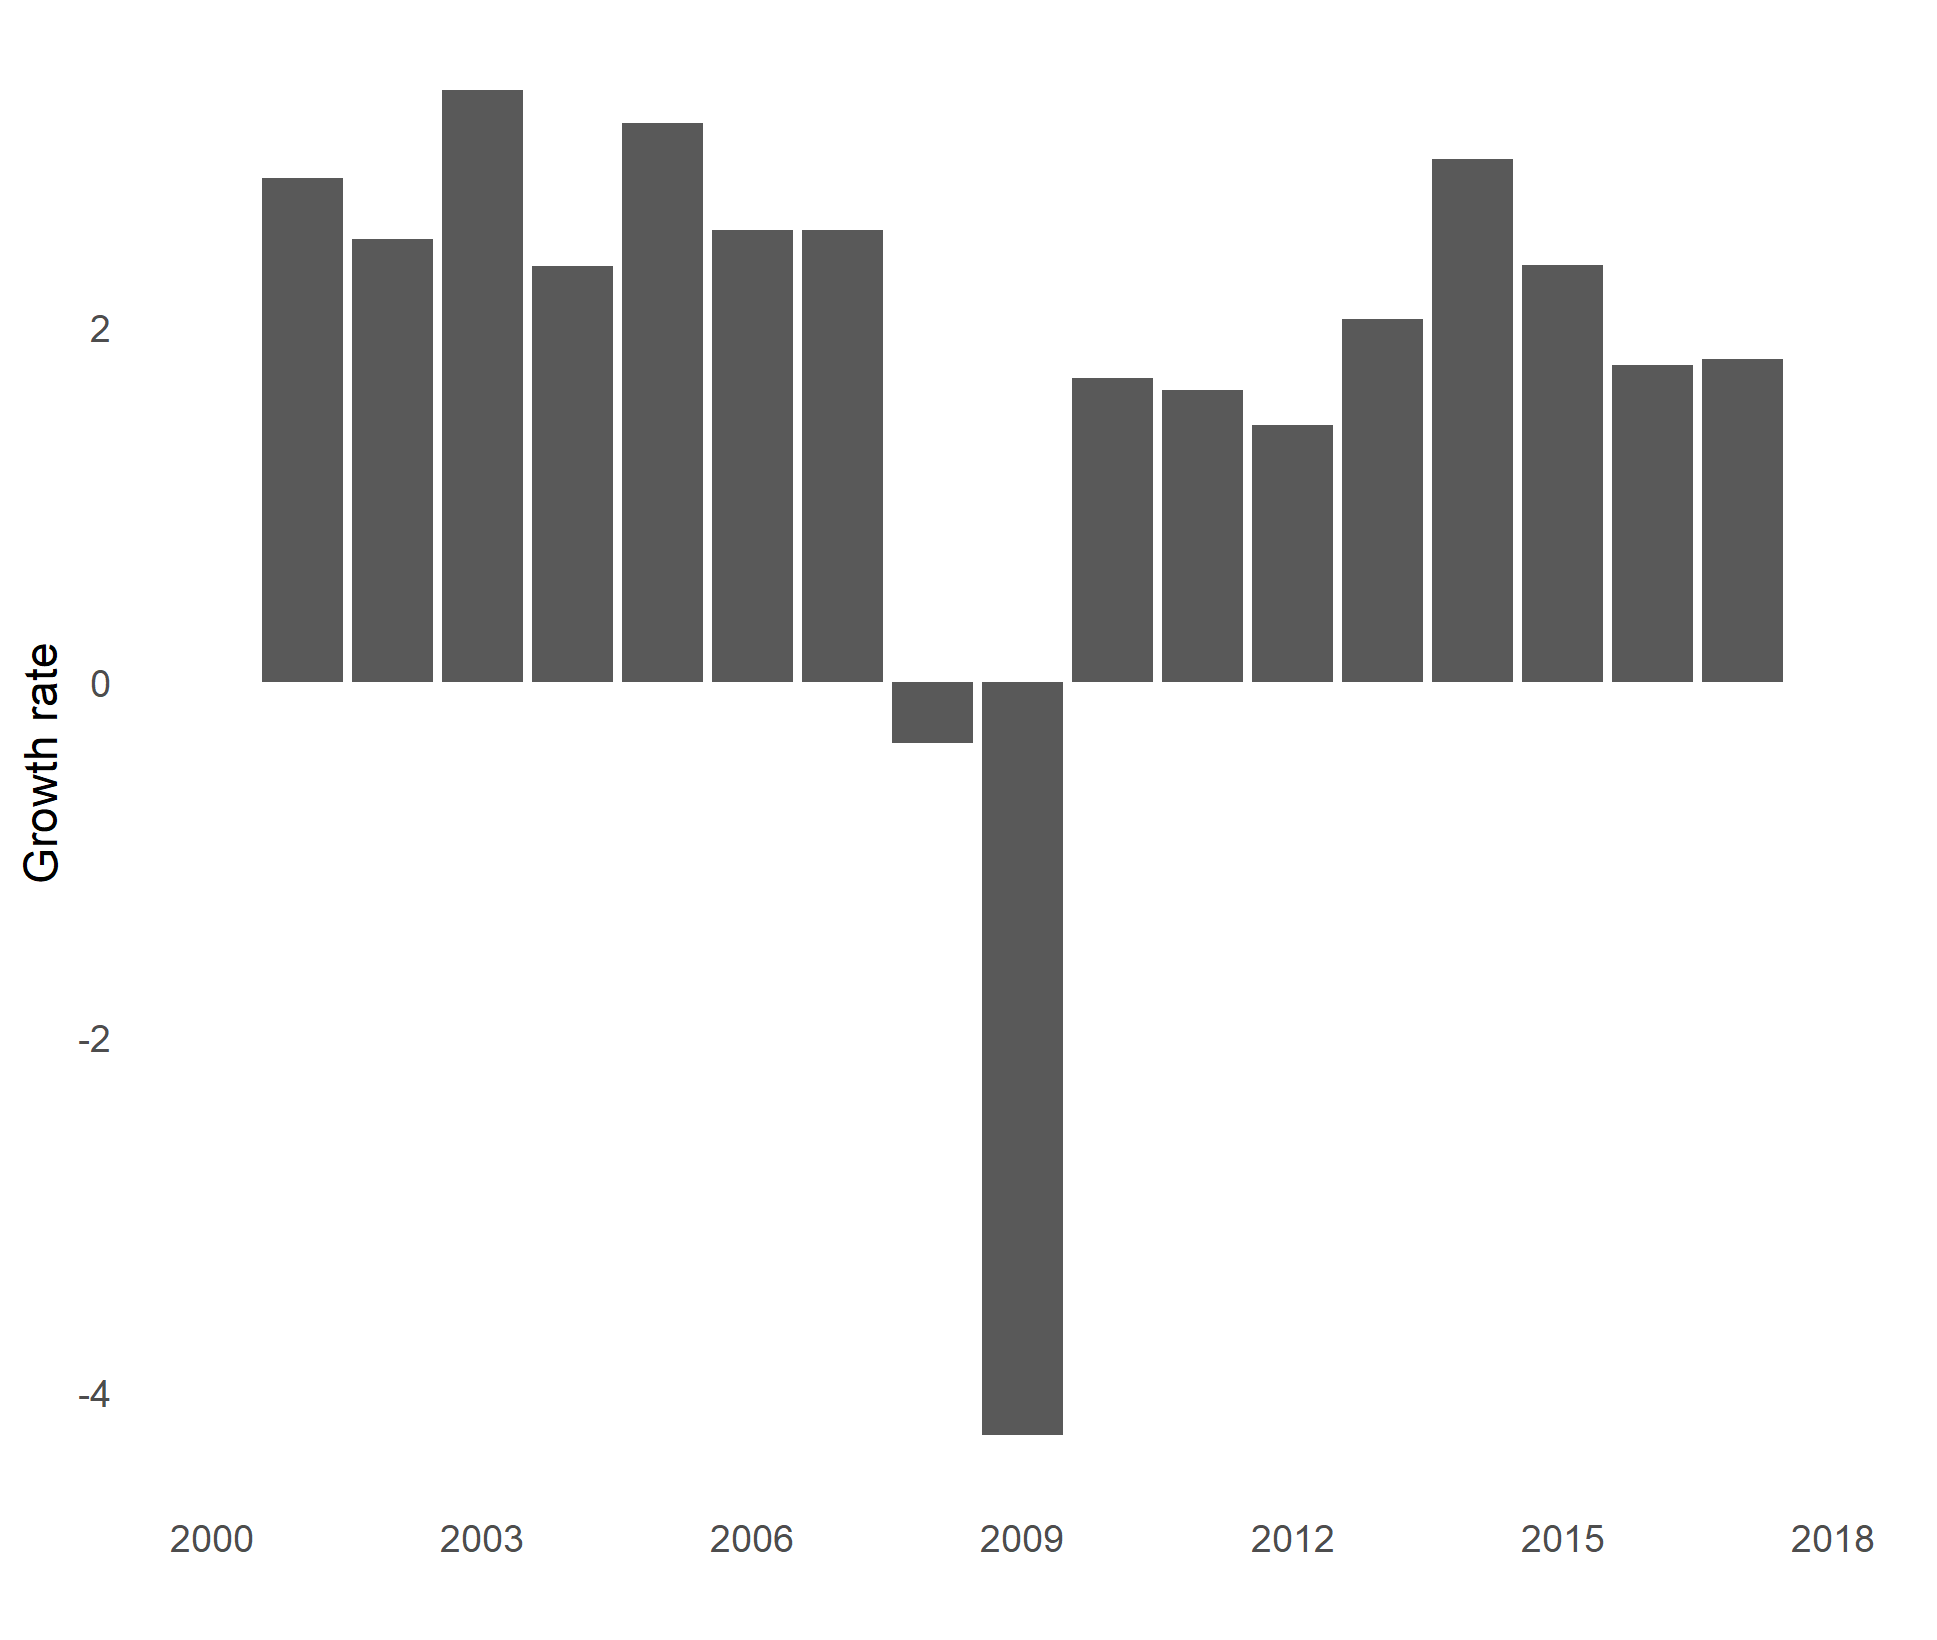
\includegraphics[width=0.8\linewidth]{_resources/chapter_gdp/fig10} 

}

\caption{Annual GDP growth rates for the UK, 2000-2018. Using a bar  chart. Source: OECD. The GDP level is measured in terms of the 2017 price level.}\label{fig:gdp13}
\end{figure}

\hypertarget{decompose-growth}{%
\subsubsection{Decompose growth}\label{decompose-growth}}

We can use each of the GDP measurement approaches above to decompose the overall GDP growth. Using the expenditure approach, we could calculate the overall GDP growth as follows:

\begin{align}
growth\text{ }rate=&growth\text{ }in\text{ }I\times I's\text{ }share\text{ }of\text{ }GDP\\
                   &+growth\text{ }in\text{ }G\times G's\text{ }share\text{ }of\text{ }GDP\\
                   &+growth\text{ }in\text{ }C\times C's\text{ }share\text{ }of\text{ }GDP\\
                   &+growth\text{ }in\text{ }NX\times NX's\text{ }share\text{ }of\text{ }GDP
\end{align}
In words, the overall GDP growth is simply a weighted average of each components growth rates. The weights are the share of overall GDP in the initial period.

Why is this useful? Say we wanted to know how household consumption \(C\) contributed to GDP growth. \(C's\) contribution is given by: \(growth\text{ }in\text{ }C\times C's\text{ }share\text{ }of\text{ }GDP\), which we can relate to the overall growth:

\begin{align}
C's\text{ }contribution\text{ }to\text{ }growth=\frac{growth\text{ }in\text{ }C\times C's\text{ }share\text{ }of\text{ }GDP}{overall\text{ }GDP\text{ }growth}
\end{align}

\hypertarget{business-cycles}{%
\subsection{Business cycles}\label{business-cycles}}

Once we know the changes in economic activity, we can start characterizing periods by terms such as business cycles, booms, overheating and recessions. The actual definitions of these concepts are considerably less clear. The US National Bureau of Economic Research has a ``Business Cycle Dating Committee'' that specifies the chronology of the US business cycles. The committee does not have a fixed definition of recessions Instead the combine real GDP, with data on the labour market and data on income. However, their definitions of recessions often coincide with a definition based on two consecutive quarters of decline in real GDP.

How exactly expansions and recessions are identified varies from country to country, but in the European Union we typically define a recession as two successive quarters of negative economic growth. A business cycle is typically defined as the period from a boom to recession and back to boom, in other words, from peak to peak. Figure \ref{fig:gdp12} shows annual levels, and we clearly see a drop in real output in 2008 and 2009. In terms of quarters, the growth rate was negative from the second quarter in 2008 to the second quarter in 2009.

\begin{myblock}
\textbf{GDP and business cycles}

\begin{itemize}
\tightlist
\item
  An economic recession is the period from peak economic activity to the
  lowest level of economic activity.
\item
  An economic expansion is the period from the lowest level of economic
  activity to the highest level of economic activity.
\item
  The economic cycle of recessions and expansions is called business
  cycles.
\item
  There is no general stringent definition of a recession, but two
  consecutive quarters of decline in real GDP is often seen as a sign of
  of a recession.
\end{itemize}
\end{myblock}

\hypertarget{gdp-per-capita}{%
\subsection{GDP per capita}\label{gdp-per-capita}}

While GDP growth rates are used across time, we are sometimes also interested in comparing across regions or countries. First, we could be interested in identifying regional recessions and expansions. Second, we could be interested in comparing the level of economic activity per capita. To achieve the latter, we divide data on total GDP for each region or country and divide by the number of residents in the region or country. Figure \ref{fig:gdp14} shows the economic activity per person in 2015. We have adjusted the price levels to be comparable across time and space. In this chart the values correspond to the price level of 2017 and we have adjusted all national values to the US price level and show the values in US dollars. To be clear, we do not simply use the exchange rate to translate the national currencies, but we also take differences in price levels across countries into account. Luxembourg has, by far, the highest level of economic activity per person, followed by Ireland and Switzerland. Of the OECD data with available data, Chile has the lowest GDP per person.

\begin{figure}

{\centering 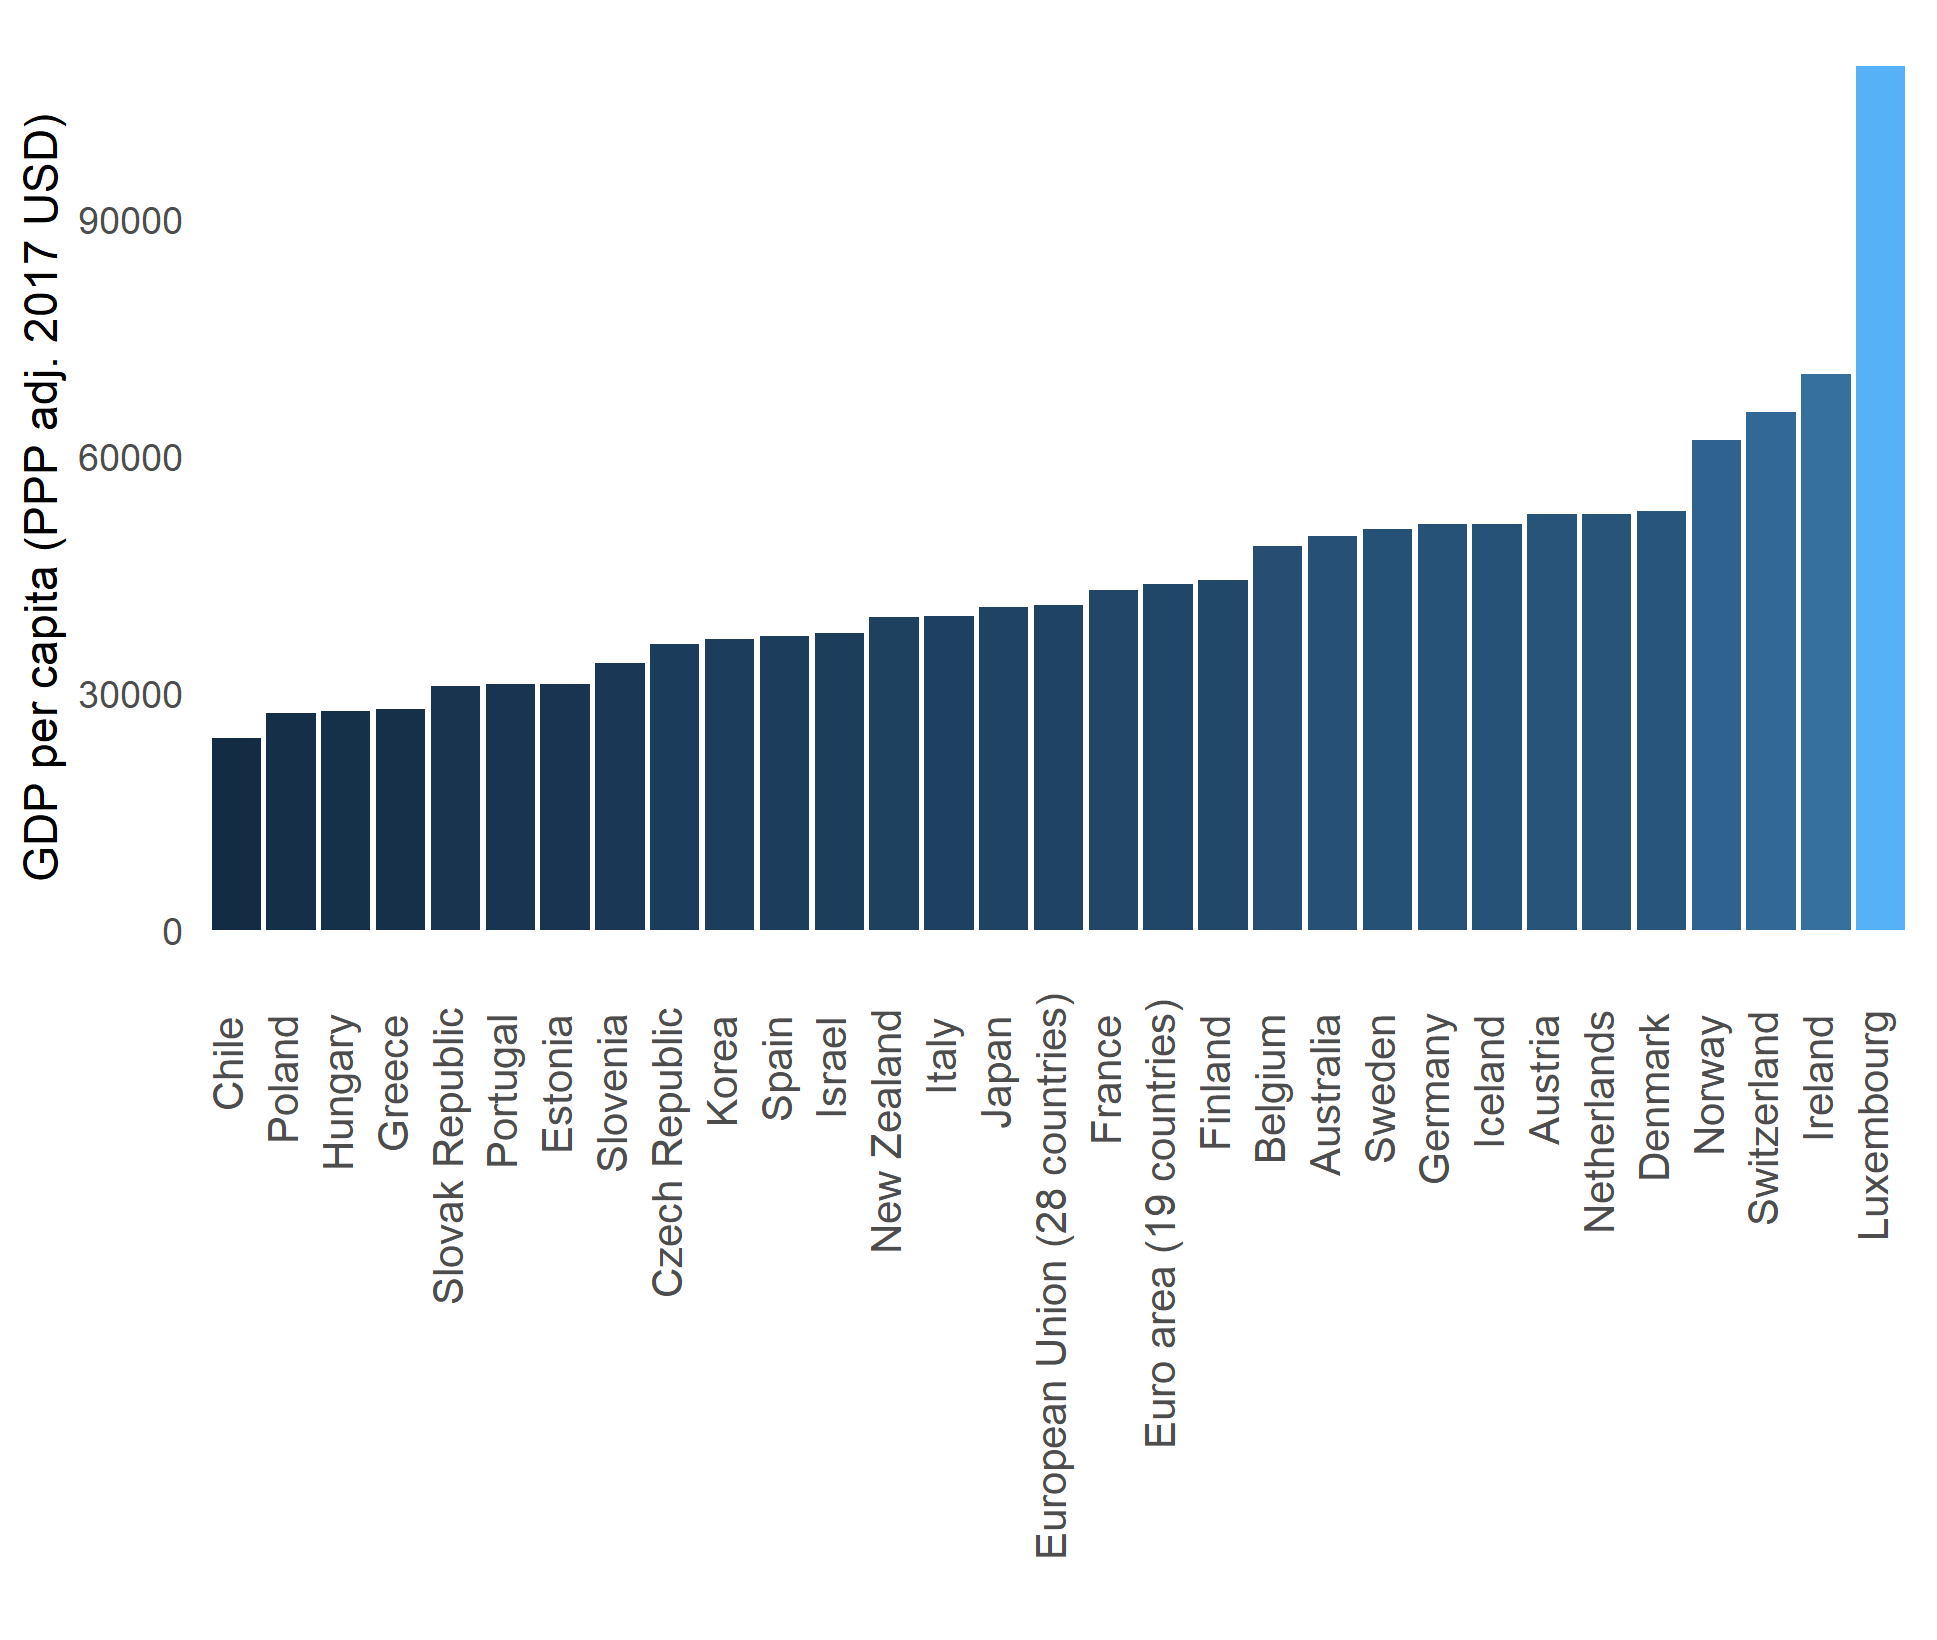
\includegraphics[width=0.8\linewidth]{_resources/chapter_gdp/fig11} 

}

\caption{GDP per capita for selected countries in 2015, measured in 2017 USD - PPP adjusted. Source: OECD. }\label{fig:gdp14}
\end{figure}

Figure \ref{fig:gdp15} shows the relative change in real economic activity per person from 2000 to 2015. Most countries increased the output per person, but not all.

\begin{figure}

{\centering 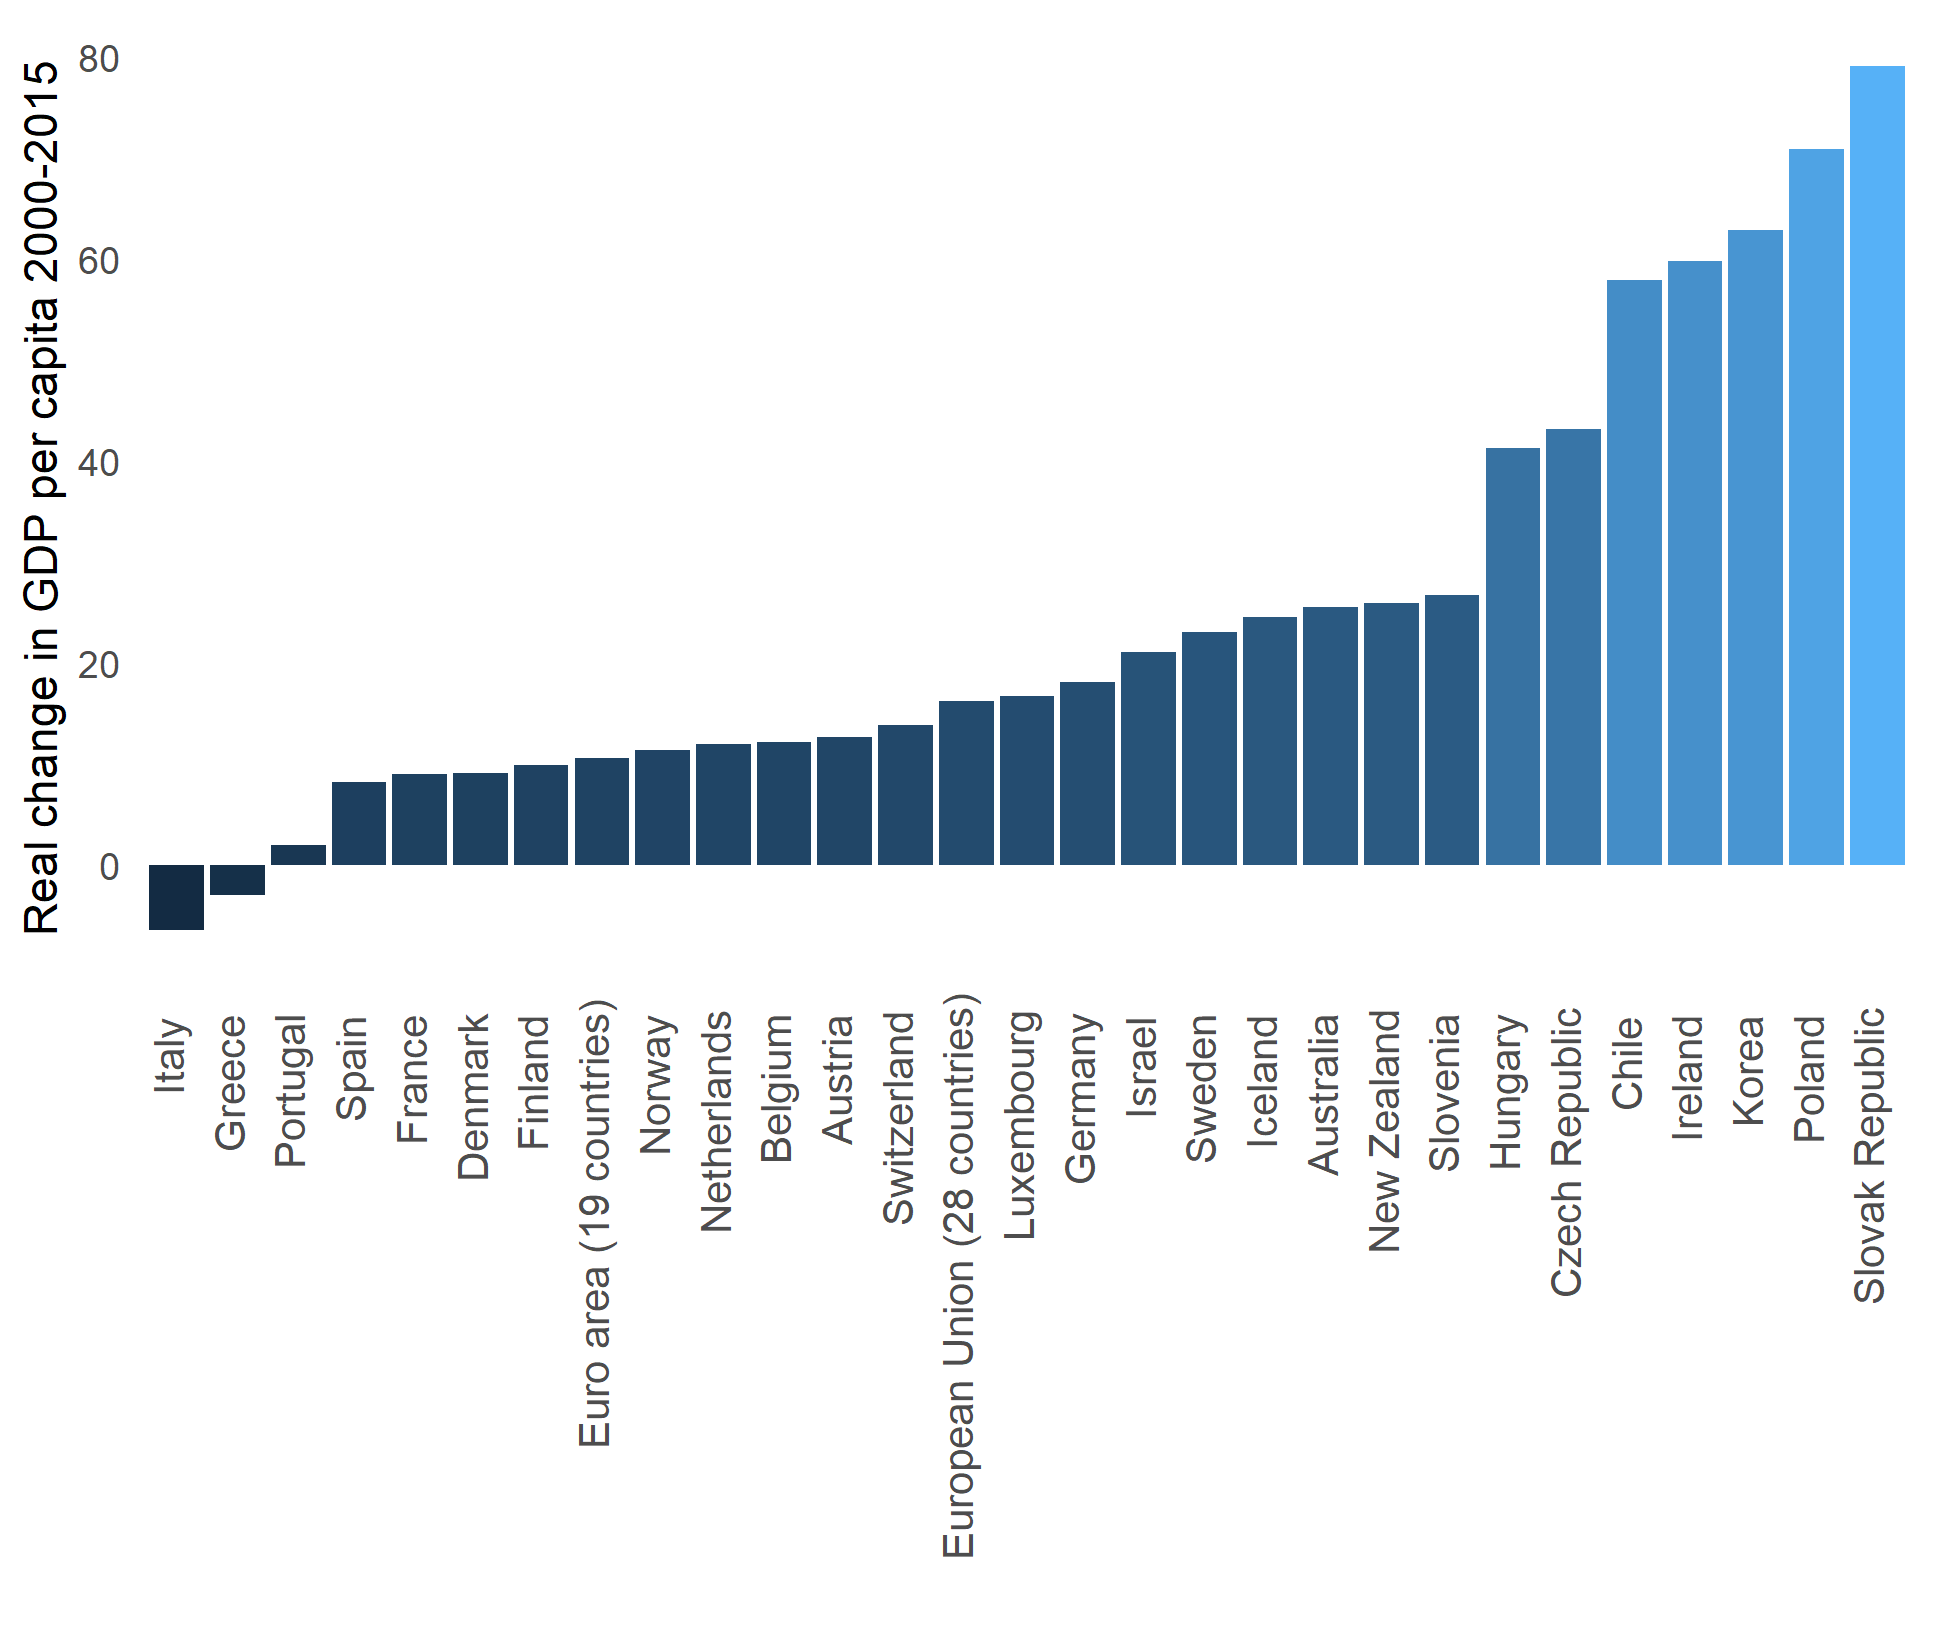
\includegraphics[width=0.8\linewidth]{_resources/chapter_gdp/fig12} 

}

\caption{Real change in GDP per capita for selected countries 2000-2015, real values measured  in 2017 USD - PPP adjusted. Source: OECD.  }\label{fig:gdp15}
\end{figure}

\hypertarget{productivity}{%
\subsection{Productivity}\label{productivity}}

Productivity is a measure of how much we can produce relative to the resources used in the production. A higher productivity means that we produce more given resources (or produce the same with less resources).

A very common approach is to measure the Gross Value Added per worker or per hours worked. A higher value then suggests that we can produce a greater value added with less labor inputs. However, we could also consider other inputs such as capital. However, the most simple approach is probably GDP per worker. This is closely related to GDP capita, which we discussed above, but in this approach we only consider the individuals who are on the labor market. Using this approach we can provide a crude but straightforward indicator for the labor productivity of a country. Changes in productivity are often the first step in understanding changes in economic activity.

\hypertarget{the-balance-of-trade}{%
\subsection{The balance of trade}\label{the-balance-of-trade}}

The balance of trade is the difference between exports and imports, also called net exports and denoted \(NX\):

\begin{align}
  NX=X-M
\end{align}

\begin{itemize}
\tightlist
\item
  \emph{NX} is the balance of trade or net exports.
\item
  \emph{X} is goods and services produced domestically but consumed abroad (Exports)
\item
  \emph{M} is goods and services produced abroad and consumed domestically (Imports).
\end{itemize}

If the balance of trade is positive it means that a country has a trade surplus, because it exports more than it imports. If a country imports more than it exports, in other words, when the trade balance is negative, the country has a trade deficit.

\hypertarget{balance-of-payments}{%
\subsection{Balance of payments}\label{balance-of-payments}}

The balance of payments (BoP) captures the overall transactions between a country and the rest of the world. According to the BoP the the sum of the current account, financial account and capital account has to be zero.

\begin{itemize}
\tightlist
\item
  The current account consists of the the balance of trade (as defined above) and the income balance (income earned abroad from domestic residents minus income earned by foreign residents).
\item
  The capital account captures international capital transfers.
\item
  The balancing item captures statistical inaccuracies.
\end{itemize}

\begin{align}
  \text{current account}+\text{capital account}+\text{balancing item}=0 
\end{align}

Let's consider an example: If we go to Germany on holiday and spend 10£ in restaurants and hotels using our English credit card, we are causing a 10£ debit on the trade balance. Let's say that we also export some English Breakfast tea for the value of 100£ to Germany. This is noted as a 100£ credit on the trade balance. The balance of trade is then \(100£-10£=+90£\). We don't earn anything abroad and no foreigner earned something in England. The current account would then be \(+90£\).

Now let us look at the capital account. The 10£ spent abroad using our English credit card will be recorded as a credit in our capital account as an investments. If we also buy some German stocks for say 15£, then these stocks will appear in debit as ``portfolio investment''. However, because we use our English credit card to buy these stocks, the 15£ will also appear on our capital account as a credit (just like the hotel and restaurant shopping). Finally, the trade credit payment from the German tea buyer is recorded in the financial accounts as a debit. The net capital account is then \(25£-115£=-90£\). As expected, the sum of the current account plus the capital account is zero. This occurs by definition through the double entry accounting framework (each entry is entered both as a debit or a credit).

It is common to separate out ``financial account'' from the capital account and use this extended definition:
\begin{align}
  \text{current account}+\text{capital account}+\text{financial account}+\text{balancing item}=0
\end{align}

\hypertarget{summary}{%
\section{Summary}\label{summary}}

So what should you take away from this chapter?

\begin{itemize}
\tightlist
\item
  What GDP and GNI are.
\item
  How GDP and GNI are measured.
\item
  The difference between real and nominal GDP.
\item
  How to calculate growth rates.
\item
  Identifying business cycles.
\item
  GDP per capita and productivity measures
\item
  Balance of Trade and Payments.
\end{itemize}

\hypertarget{measuring-well-being}{%
\chapter{Measuring Well-Being}\label{measuring-well-being}}

\hypertarget{about-this-chapter-2}{%
\section{About this chapter}\label{about-this-chapter-2}}

We will now follow up on some of the issues on measuring well-being raised in the last chapter. In the last chapter we learned how GDP is a measure of economic activity and how it is (mis)used as a measure of well-being. In this chapter we discuss the problems with using GDP as a well-being measure, what well-being is, and how we can measure it.

\hypertarget{intended-learning-outcomes-2}{%
\subsection{Intended learning outcomes}\label{intended-learning-outcomes-2}}

After reading this chapter you should be able to:

\begin{itemize}
\tightlist
\item
  Explain the problems of using GDP as a well-being measure.
\item
  Explain and identify subjective and objective measures of well-being.
\item
  Use publicly available measures of well-being and explain how they are created and relate to each other.
\item
  Use scatter plots and understand how we can combine several variables in one measure.
\end{itemize}

\hypertarget{what-is-well-being}{%
\section{What is well-being?}\label{what-is-well-being}}

One of the reason for why the GDP is so popular is that it has a more or less globally accepted standard way of quantifying economic activity. Very few variables are as standardized as GDP (although there are some variation in what is included in the GDP measure). We use GDP because the GDP is available and because the GDP is comparable across countries and regions. Not even definition of unemployment rate is as standardized as the measure of GDP. But we now know what the GDP captures and what should use it for and what we shouldn't use it for. It is a measure of economic activity, not a measure of well-being. But what is well-being? What is welfare?

The first challenge is to agree on what we want to measure and what we want to call it. Is it well-being, happiness, welfare or quality of life. The ``Stiglitz report'' \citep{stiglitz2010report} (discussed below) uses the term ``Quality of Life'' and state the following:

\begin{quote}
"While a long tradition of philosophical thought has addressed the issues of what gives
life its quality, recent advances in research have led to measures that are both new and
credible. This research suggests that the need to move beyond measures of economic
resources is not limited to developing countries (the traditional focus of much work on
human development in the past) but is even more salient for rich industrialised countries.
These measures, while not replacing conventional economic indicators, provide an
opportunity to enrich policy discussions and to inform people's view of the conditions of the
communities where they live. More importantly, the new measures now have the potential to
move from research to standard statistical practice. While some of them reflect structural
conditions that are relatively invariant over time but that differ systematically across
countries, others are more responsive to policies and more suitable for monitoring changes
over shorter periods of time. Both types of indicator play an important role in evaluating
quality of life.
\end{quote}

\citep[page 41 in][]{stiglitz2010report}

We will go through the three conceptual approaches discussed in the Stiglitz report below and later present some measured of quality of life and well-being in practice and how they relate to the conceptual approaches.

\hypertarget{gdp-and-well-being}{%
\section{GDP and well-being}\label{gdp-and-well-being}}

\hypertarget{the-stiglitz-report}{%
\subsection{The Stiglitz Report}\label{the-stiglitz-report}}

One important milestone in the debate on measuring well-being and quality of life is the so called ``Stiglitz Report'' \citep{stiglitz2010report}, named after one of the authors, professor Joseph E. Stiglitz. The official title of the report is ``Report by the Commission on the Measurement of Economic Performance and Social Progress''. The goal of the commission behind the report was

\begin{quote}
``to identify the limits of GDP as an indicator of economic performance and social progress, including the problems with its measurement; to consider what additional information might be required for the production of more
relevant indicators of social progress; to assess the feasibility of alternative measurement
tools, and to discuss how to present the statistical information in an appropriate way.''
\end{quote}

page 7 in \citep{stiglitz2010report}.

The report provides detailed examples and criticism of GDP as a measure of well-being and social progress as well, as discussed, conceptual approaches to measure well-being. We will first briefly discuss some of the most prominent criticism of GDP as a measure of well-being and then return to how we could do a better job.

\hypertarget{criticism-of-gdp-as-a-well-being-measure}{%
\subsection{Criticism of GDP as a well-being measure}\label{criticism-of-gdp-as-a-well-being-measure}}

\begin{enumerate}
\def\labelenumi{\arabic{enumi}.}
\item
  GDP is a poor measure of human welfare

  The first criticism is probably the most-known critique: GDP measures consumption of goods and services (the expenditure approach), and while these aspects might be correlated with quality of life, there are many aspects of utility and well-being that are not captured by GDP. To list a few:

  \begin{itemize}
  \tightlist
  \item
    Nature and environment (pollution)
  \item
    Education
  \item
    Health
  \item
    Crime and safety
  \end{itemize}

  Consider two countries that have an identical GDP per capita. In the first country there is almost no pollution, there are beautiful mountains, forests, lakes and beaches. In the second country there is lots of pollution and no access to nature. Moreover, in the first country life expectancy is high and the population have very few health problems. In the second country life expectancy is low and the mental and physical health of the population is very low.

  Would you say that well-being is the same in the two countries (they have the same GDP per capita)? Probably not. And GDP per capita does not capture all these elements listed above (and many elements we did not list).

  Many studies find that GDP per capita is correlated with the dimensions above. For example that higher GDP capita is associated with lower infant mortality rates. But this is not the case for all dimensions, and the question is whether it is sufficient that GDP is correlated with these aspects.
\item
  GDP ignores the distribution

  Again, consider two countries with identical GDP per capita. In the first country, some have a bit more resources than others, but very few are poor and very few are extremely rich. In the second country all inhabitants are poor, with the exception of one extremely rich person. Is the well-being the same these two countries?

  In practice we often observe GDP growth rates that affect the population unevenly. The well-educated population may benefit more from growth driven by advanced innovation than unskilled workers. The GDP per capita measure does not capture these distributional effects. Recall from the last chapter that Kusnets already mentioned the issue of not accounting for the distribution of income \citep[page 6 in][]{kuznets1934national}.
\item
  Well-being is not monotonically increasing

  Does GDP growth always make people happier? And is the effect constant? Promoting GDP growth appears to be an endless goal, but in practice, the effect of more GDP on well-being might non-linear and even non-monotonic. Going from starvation to having enough food and decent living conditions might affect well-being more than the same monetary increase for people who already have very high living standards. Moreover, there might be some certain level of saturation, after which more GDP does not lead to increases in well-being.

  Some evidence suggests that after a certain level resources, people care mostly about their relative position. This is phenomena called ``keeping up with the Joneses'', where we envy those who have more than us, and enjoy looking at those who have less than us. In such a case, a uniform increase in income for all of us has no effect on the well-being.
\end{enumerate}

\hypertarget{how-to-measure-well-being-quality-of-life}{%
\section{How to measure well-being \& quality of life}\label{how-to-measure-well-being-quality-of-life}}

\hypertarget{recommendations-from-the-stiglitz-report}{%
\subsection{Recommendations from the Stiglitz report}\label{recommendations-from-the-stiglitz-report}}

The commission the Stiglitz report identified the following three conceptual approaches to measuring quality of life:

\begin{enumerate}
\def\labelenumi{\arabic{enumi}.}
\item
  \emph{Subjective well-being}

  The key idea is that we simply ask people about their well-being and happiness with the idea that: ``that enabling people to be happy and satisfied with their life is a universal goal of human existence.'' from page 7 in \citep{stiglitz2010report}
\end{enumerate}

There are several standardized questionnaires to capture the measures above and many of them show consistent patterns:

\begin{quote}
``Research has shown that it is possible to collect meaningful and reliable data on
subjective well-being. Subjective well-being encompasses different aspects (cognitive
evaluations of one's life, positive emotions such as joy and pride, and negative emotions such as pain and worry): each of them should be measured separately to derive a more comprehensive appreciation of people's lives. Quantitative measures of these subjective aspects hold the promise of delivering not just a good measure of quality of life per se, but also a better understanding of its determinants, reaching beyond people's income and material conditions.''
\end{quote}

page 58 in \citep{stiglitz2010report}

\begin{enumerate}
\def\labelenumi{\arabic{enumi}.}
\setcounter{enumi}{1}
\item
  \emph{Capabilities}

  The second conceptual approach to measuring well-being is to measure individuals ability to pursue and realise the goals that they value (the capabilities).
\item
  \emph{Fair allocations}

  The third conceptual approach to measuring well-being is to measure the allocation of resources among people with different tastes and abilities.
\end{enumerate}

\hypertarget{operationalizing-well-being-measures}{%
\subsection{Operationalizing well-being measures}\label{operationalizing-well-being-measures}}

\hypertarget{subjective-well-being-measures}{%
\subsubsection{Subjective well-being measures}\label{subjective-well-being-measures}}

Subjective well-being measures are often divided into the following three types:

\begin{itemize}
\item
  Evaluative measures
  In this approach we ask respondents to evaluate their life satisfaction, their health, or in general their well-being. We can anchor these questions (``relative to the best possible state'' or relative to some objective state.).
\item
  Experience measures

  In this approach we ask respondents about their feelings or experiences at specific points during the day (or during the week).
\item
  Eudemonic measures

  This approach focuses on psychological aspects of individual well-being and relates to the individual's position and control over their life.
\end{itemize}

\begin{figure}

{\centering 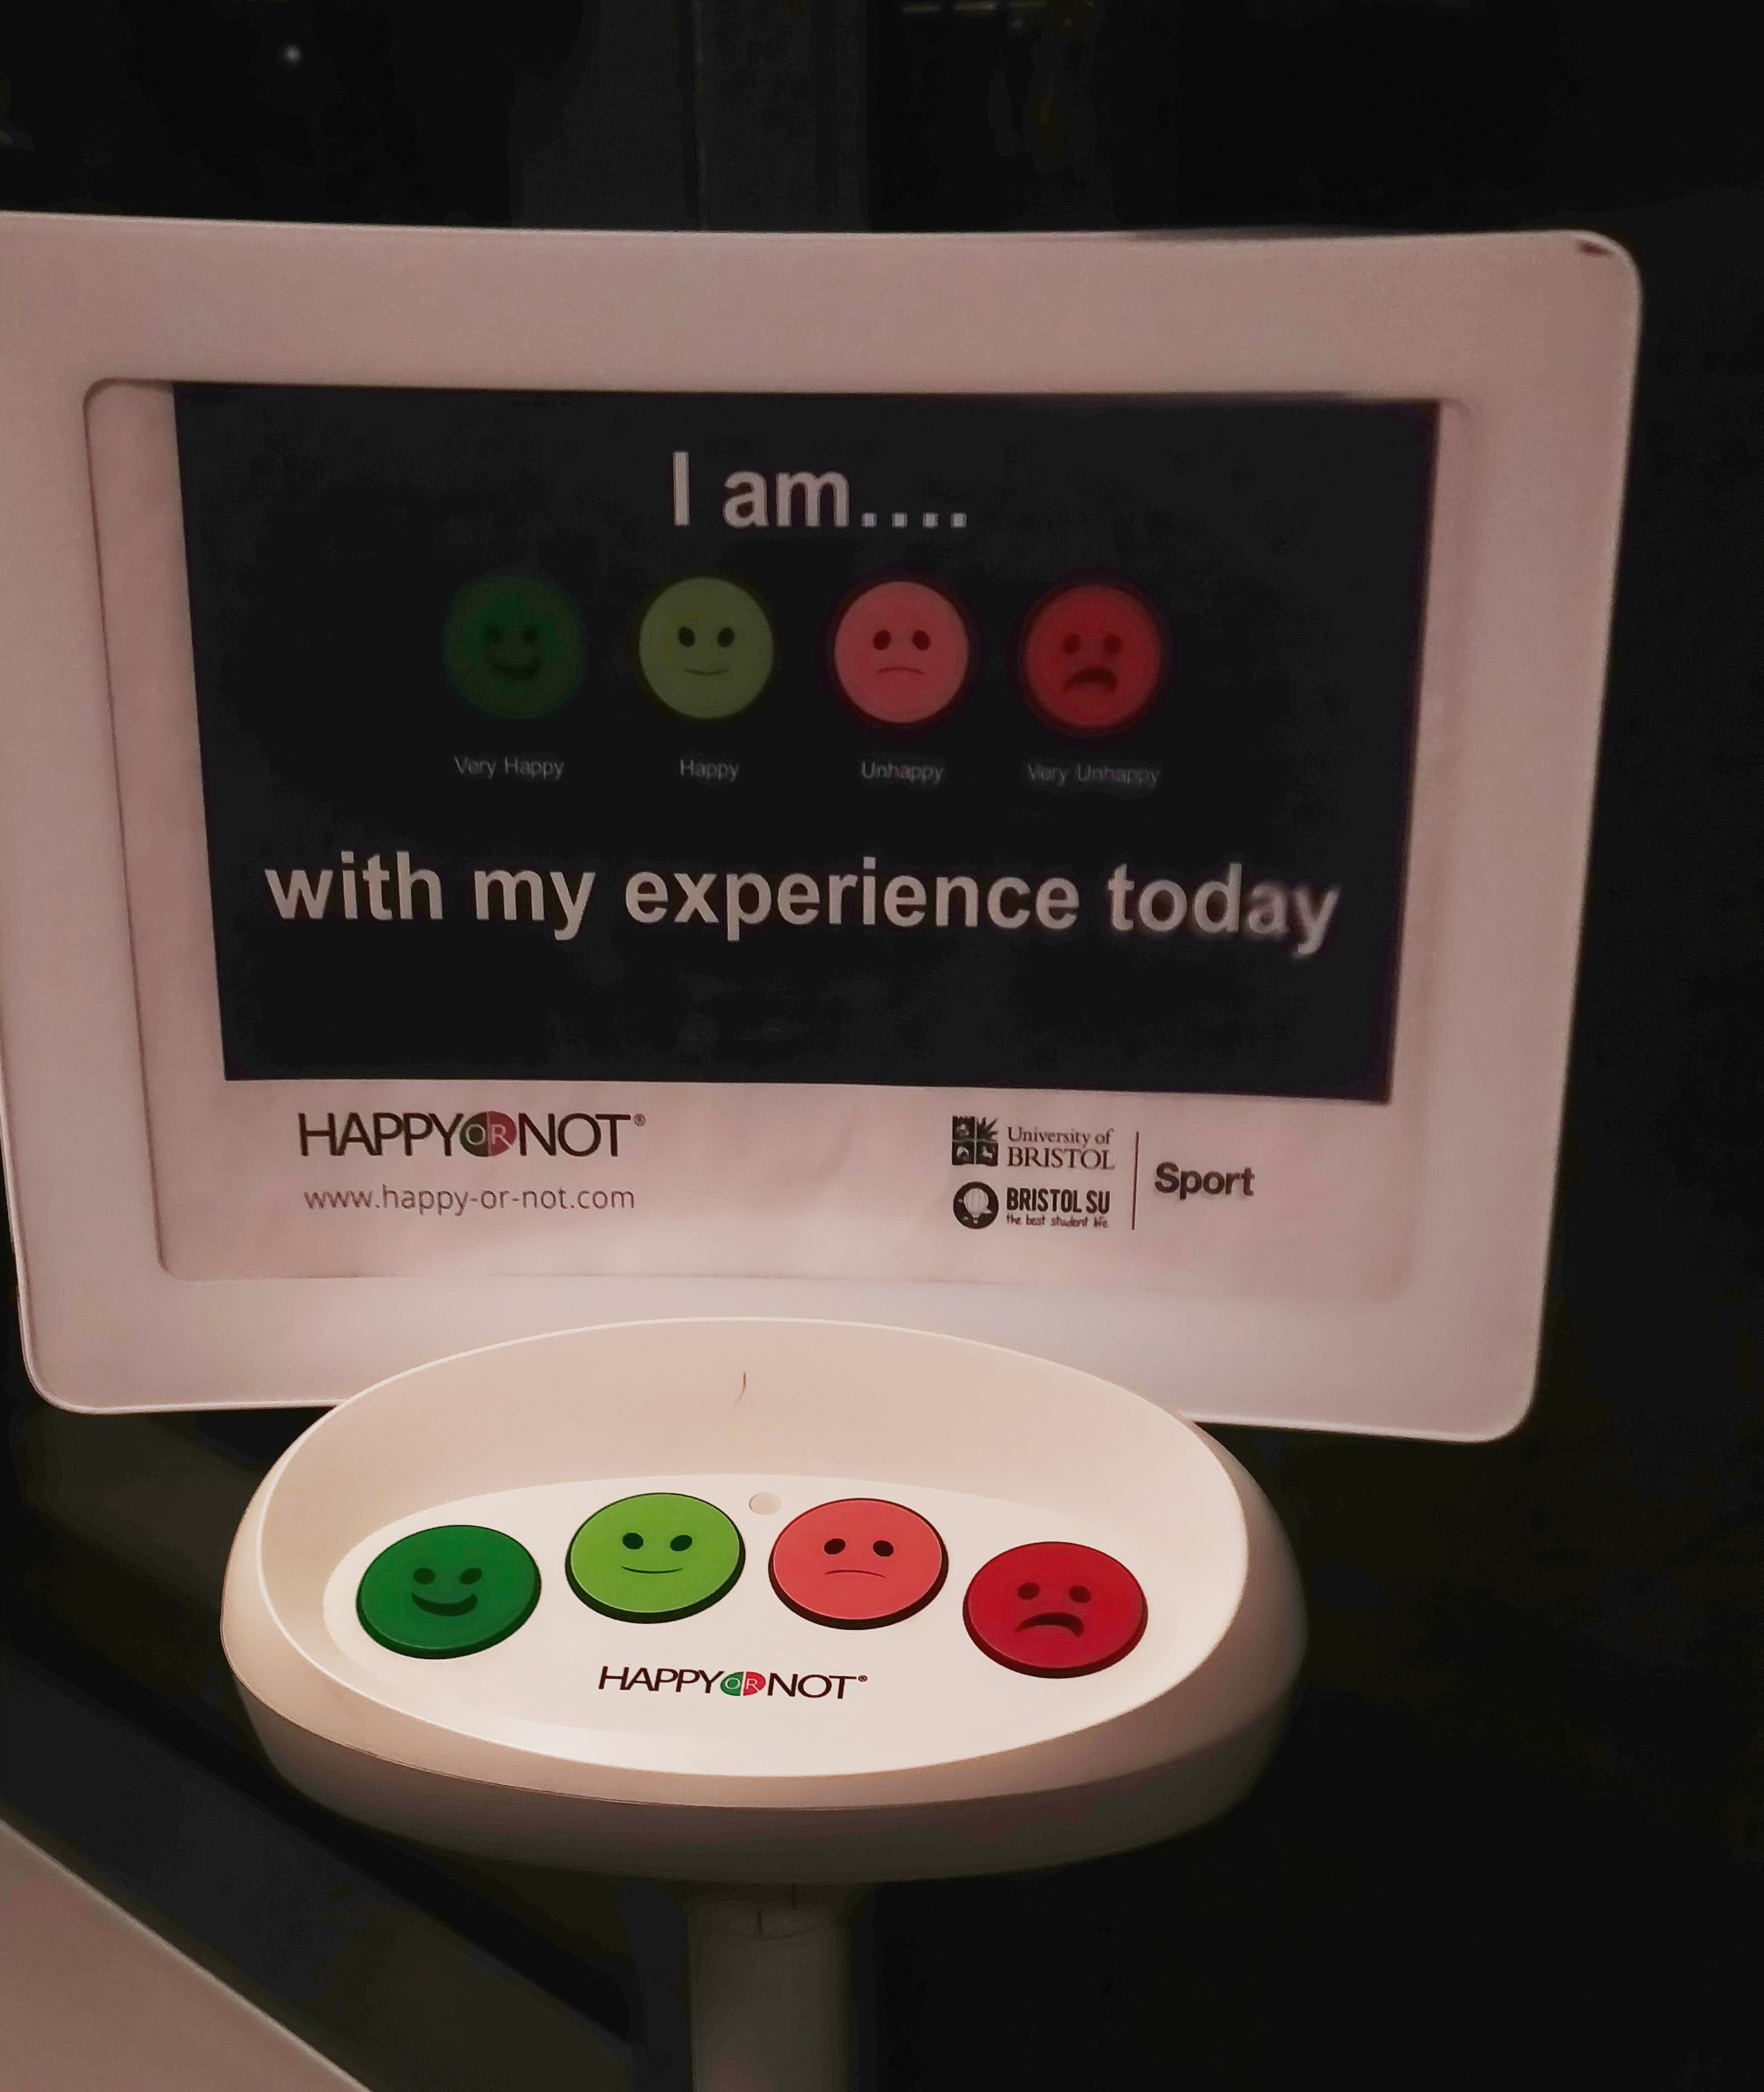
\includegraphics[width=0.7\linewidth]{_resources/chapter_wellbeing/subwb} 

}

\caption{Ask people how they feel}\label{fig:wfig2}
\end{figure}

\hypertarget{objective-well-being-measures}{%
\subsubsection{Objective well-being measures}\label{objective-well-being-measures}}

While subjective well-being typically is measured through questionnaires where we directly ask people about their their well-being, the capabilities and fair allocations approaches typically rely on ``objective measures''. However, these approaches should not be considered as ``more objective'' compared to the subjective measures. For example the choice of indicators to include depend on a normative judgement.

\begin{quote}
``The information relevant to valuing quality of life goes beyond people's self-reports and perceptions to include measures of their functionings and freedoms. While the precise list of these features inevitably rests on value judgements, there is a consensus that quality of life depends on people's health and education, their everyday activities (which include the right to a decent job and housing), their participation in the political process, the social and natural
environment in which they live, and the factors shaping their personal and economic security. Measuring all these features requires both objective and subjective data. The challenge in all these fields is to improve upon what has already been achieved, to identify gaps in available information, and to invest in statistical capacity in areas (such as time-use) where available indicators remain deficient.''
\end{quote}

page 58 in \citep{stiglitz2010report}

\hypertarget{measuring-well-being-in-practice}{%
\section{Measuring well-being in practice}\label{measuring-well-being-in-practice}}

Let us now discuss approaches to measuring well-being in practice and how they relate to the approaches discussed above.

\hypertarget{quick-guide-combining-several-variables}{%
\subsection{Quick guide: Combining several variables}\label{quick-guide-combining-several-variables}}

How can we create a well-being measure that combines measures of subjective well-being, measures of health, education, environment, crime in one statistic?

When working with topics such as global development or well-being, we are often interested in aggregating several variables to obtain one variable. Many of the strategies to achieve this are beyond the scope of this unit, but you should be aware of these methods.

\begin{enumerate}
\def\labelenumi{\arabic{enumi}.}
\item
  Creating an index

  Well-being measures such as the Human Development are s based on aggregating three individual indices by means of the \textbf{geometric mean}.
\end{enumerate}

\begin{align}
   HDI=(LEI\times EI\times II)^{1/3}
\end{align}

Where \(LEI\) is the life expectancy index, \(EI\) is the education index, and \(II\) is the income index. Each of these indices are measured on a scale from 0 to 1, where the raw variables are related to some ``max'' value. For example for life expectancy, the maximum is 85 (i.e.~an index value of 1) and the minimum is 20 (i.e.~an index value of 0). A standard formula of measuring the individual index is as follows:

\begin{align}
   I=\frac{Y-Y_{MIN}}{Y_{MAX}-Y_{MIN}}.
\end{align}

To create an index, just like the HDI, we therefore first convert each variable to be on a scale between 0 and 1 using the formula above, and we then compute the geometric mean across all Indexes \(i\):

\begin{align}
   \text{Aggregate Index}=\left(\prod_{i=1}^N I_i\right)^{1/N}
\end{align}

\begin{enumerate}
\def\labelenumi{\arabic{enumi}.}
\setcounter{enumi}{1}
\tightlist
\item
  Principal Component Analysis and Factor Analysis
\end{enumerate}

Principal component analysis (PCA) and Factor analysis are methods to reduce the dimensionality of data. These approaches are very often used in regressions, when you want to reduce the number of variables. With these method you can identify a set of \emph{components} or \emph{factors} that describe the variation in the data. The goal is typically to identify a set of components and factors that are smaller than the number of variables used.

Intuitively speaking, the goal is to identify variables that ``move in the same direction''. Imagine that you have a dataset with 25 behavioural measures of a child. Five of these measures relate to the child's peer relations. When one of these variables go up, the other four also tend to go up. Another five variables might capture the child's level of hyperactivity and inattention, again, if one of the five variables goes up, the other four also tend to go up. We have those identified two separate components, that each cover five underlying variables.

Factor analysis and principal component analysis are two distinct methods. Factor analysis is more based on theories of underlying latent (unobserved) variables, while principal component analysis is more based the objective to reduce the number of dimensions (number of variables) in the data.

\begin{myblock}
\textbf{Reducing the dimensions}

Because well-being depends on several aspects, such as health,
environment, income and education, it is hard to compare across time and
space. There are simply too many ``dimensions''. We would like to reduce
the well-being to one variable, to one dimension. There are several
approaches to combine several variables in one variable. The following
two methods are very common:

\begin{itemize}
\tightlist
\item
  A \emph{An index based on a geometric mean}
\item
  A \emph{Principal component analysis}
\end{itemize}
\end{myblock}

\hypertarget{the-human-development-index-un}{%
\subsection{The Human Development Index (UN)}\label{the-human-development-index-un}}

The Human Development Index (HDI) is developed by the United Nations Development Programme (UNDP). The index is an example of combining several objective indicators of well-being in one measure. The index consists of the three dimensions:

\begin{itemize}
\tightlist
\item
  Life expectancy index
\item
  Education index
\item
  Income index.
\end{itemize}

the HDI is created by the geometric mean of the the three indices above. There ahas been some changes in the HDI definition over time. Data is available for the period 1995-2015 for many countries across the world. The data can be downloaded from the website of the United Nations: \href{http://worldhappiness.report/}{UN}.

\hypertarget{world-happiness-report}{%
\subsection{World Happiness Report}\label{world-happiness-report}}

Published by the United Nations since 2012, the World Happiness Report uses data from the Gallup World Poll to describe global happiness patterns, by linking these data to specific topics (for example migration). The data is available for download here: \href{http://worldhappiness.report/}{World Happiness Report}.

\hypertarget{oecd-better-life-index}{%
\subsection{OECD Better Life Index}\label{oecd-better-life-index}}

The OECD has computed the ``Better Life Index'' since 2013. The index is a combination of subjective and objective indicators that captures 11 dimensions of well-being: housing, income, jobs, community, education, environment, civic engagement, health, life satisfaction, safety and work-life balance. The data is available both as a total, by subgroups (men and women) and by distribution (low vs.~high). The data can be downloaded from the OECD website: \href{https://stats.oecd.org/}{OECD}.

\hypertarget{ons-measuring-national-well-being}{%
\subsection{ONS Measuring National Well-being}\label{ons-measuring-national-well-being}}

The UK office for National Statistics collects data on well-being measures. These data are a combination of subjective and objective indicators and capture personal well-being, relationships, health, what we do, where we life, personal finance, the economy, education and skills, governance, and the natural environment. The data is available both on aggregated level, and also on a regional level from the ONS website: \href{https://www.ons.gov.uk/peoplepopulationandcommunity/well-being}{ONS}.

\hypertarget{quality-of-life-indicators}{%
\subsection{Quality of life indicators}\label{quality-of-life-indicators}}

Eurostat publishes various statistics related to quality of life. They have identified nine indicators to capture quality of life. These aspects are also a mix of subjective and objective indicators. A description of their approach and links to data is available here: \href{http://ec.europa.eu/eurostat/statistics-explained/index.php/Quality_of_life_indicators_-_measuring_quality_of_life\#Overall_experience_of_life}{eurostat}.

\hypertarget{why-is-the-gdp-used-anyway}{%
\section{Why is the GDP used anyway?}\label{why-is-the-gdp-used-anyway}}

Why is GDP so important in policy making despite the criticism above? First of all, as disucssed above. GDP has the advantage of being available and being standardized. Secondly, it is correlated with many of the well-being measures discussed above. In Figure \ref{fig:wb1} we combine data on GDP per capita and the quality of life measures from Eurostat. What do you think of relationship? Do you recognize any of the criticism of GDP as a well-being measure?

\begin{figure}

{\centering 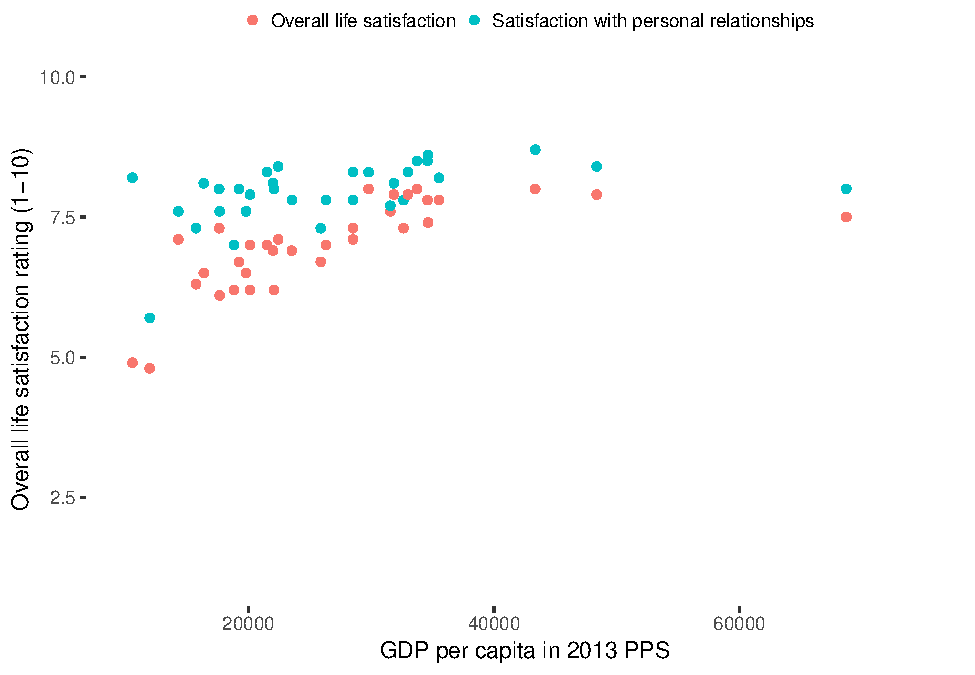
\includegraphics[width=0.95\linewidth]{book_files/figure-latex/wb1-1} 

}

\caption{Figure 1: GDP per capita and subjective well-being in 2013. Source: Eurostat}\label{fig:wb1}
\end{figure}

To assess the relationship between the two variables, GDP per capita and Subjective Well-Being we used a scatter plot. A scatter plot is like an unconnected line chart where the vertical and horisontal positions represent the values of respectively the variables on the vertical (y) axis and horisontal axis (x). Scatter plots are very powerful tools to show relationships between variables, especially when we have a lot of data.

\hypertarget{summary-1}{%
\section{Summary}\label{summary-1}}

In this chapter we covered the following topics:

\begin{itemize}
\tightlist
\item
  What are the problems of using GDP as a well-being measure.
\item
  What is the ``Stiglitz report''
\item
  How can measure well-being in practice?
\item
  What well-being measures exist?
\item
  How can we combine several variables into one variable?
\item
  What can we use scatter plots for?
\end{itemize}

\hypertarget{life-and-death}{%
\chapter{Life and Death}\label{life-and-death}}

\hypertarget{what-this-chapter-is-about}{%
\section{What this chapter is about}\label{what-this-chapter-is-about}}

In earlier chapters we've discussed how Gross Domestic Product measures economic activity, and how other measures should be included to give a comprehensive measure of quality of life. Many of the available well-being measures use ``life expectancy'' as an (objective) indicator of health conditions. We should therefore be able to calculate life expectancy and explain the assumptions under which it is created. Moreover, fertility behavior is clearly linked to well-being. Fertility measures are rarely used directly in indexes, but they are nevertheless important for social scientists. First of all, there might be a link between between economic conditions, social conditions and fertility behavior. Could you come up with an explanation why? (You will be asked to do this in the exercises). Secondly, fertility behavior (and life expectancy) affects the age composition of the population, which is directly relevant for public policies. After reading this chapter you should be able to:

\begin{itemize}
\tightlist
\item
  Use standard measures of fertility

  \begin{itemize}
  \tightlist
  \item
    The Age-Specific Fertility Rate
  \item
    The Total Fertility Rate
  \item
    The General Fertility Rate
  \item
    The Crude Birth Rate
  \end{itemize}
\item
  Create life tables
\item
  Calculate life expectancy
\end{itemize}

\hypertarget{describing-fertility-trends}{%
\section{Describing fertility trends}\label{describing-fertility-trends}}

Now we know that the population increase of the United Kingdom is both due to positive net migration flows and positive reproduction flows. We can go one step deeper and assess the changes in births in the United Kingdom. To investigate this we can make use of some of the standard definitions for describing fertility in a population:

\begin{itemize}
\item
  \emph{Age Specific Fertility Rate (ASFR)}

  The number of live births per woman in a specific age group.

  \begin{align}
        ASFR_a=\frac{\text{Number of births to women in age group} a}{\text{Number of  women in age     group} a}
    \end{align}
\item
  \emph{Total Fertility Rate (TFR)}:

  The number of children born per woman if she were to pass through the childbearing years (typically set to: 15-44y or 15-49y) bearing children according to a current age-specific fertility rates.

  \begin{align}
    TFR=\sum_{a=15}^{44}ASFR_a
  \end{align}
\item
  \emph{General Fertility Rate (GFR)}

  All live births per woman in the childbearing ages (also typically per 1000 women).

  \begin{align}
    GFR=\frac{\text{Number of births }}{\text{Number of  women in childbearing age} }
  \end{align}
\item
  \emph{Crude Birth Rate (CBR)}
\end{itemize}

All live births per 1000 population of all ages
\begin{align}
    CBR=\frac{\text{Number of births }}{\text{Population size} }
  \end{align}

\hypertarget{data-requirements}{%
\subsection{Data requirements}\label{data-requirements}}

In order to be able to calculate the fertility rates described above we need data on: (1) the number of live births by the age of the mother, (2) the number of women by age, (3) number of people in the population. Merging these data from Eurostat we can create Figure \ref{fig:death1}), which shows the development in the number of live and still births. Note that we again show two series with different scales in the same Figure using two different vertical axes. Why did we combine these two graphs, and why do they have very different scales?

\hypertarget{relating-the-fertility-measures-to-each-other}{%
\subsection{Relating the fertility measures to each other}\label{relating-the-fertility-measures-to-each-other}}

Why do we have different fertility measures and what do they say? When thinking about fertility in layman terms, we typically think about the number of children a woman will have in her life. It is an easily understandable hypothetical measure of completed fertility, which is captured by the Total Fertility Rate (TFR). It is hypothetical because we sum the age-specific fertility measures across ages at a given point in time. Any woman in this sample will of course only be included in one of the age specific fertility rates and contribute to that value. We impute the total fertility rate by summing over a lot of different age groups, who will be at different ages in different points in time.

The General Fertility Rate (GFR) on the other hand gives information about the number of new children relative to the number of women in childbearing ages. It is therefore an actual (and not a hypothetical) number. This is a refinement over the crude birth rate by taking into account the share of women in the population. To sum up, we should use the Total Fertility Rate to describe the fertility (behavior) and General Fertility Rate to describe the ``number of individuals'' added to the society. How does the General Fertility Rate relate to the Total Fertility Rate?

\emph{From GFR to TFR:} A General Fertility Rate of about 60 (like at the end of the period in Figure \ref{fig:death1}) shows that 1000 women had 60 children in that year. Or that 1 woman on average had 0.06 children on average this year. But this of course only considers one year. In our calculations we used the age group 15 to 45 (although 15 to 49 is also common), which means that we considered 31 years of a woman's life. We can therefore multiply the 0.06 by 31 to get 1.83 which would be the average number of children a woman would have if all years were like this year. However, the TFR at the end of the period shown in Figure \ref{fig:death1} was 1.73. Why do these number differ? There are two reasons: Firstly, the number of woman in each age group differs. Secondly, the fertility rates differ by age. If one of these aspects is constant, the Total Fertility Rate will be the same as the General Fertility rate.

\begin{itemize}
\tightlist
\item
  TFR \& GFR are the same when:
\item
  The number of women in each age group is constant.
\item
  The ASFRs are the same.
\end{itemize}

\begin{figure}

{\centering 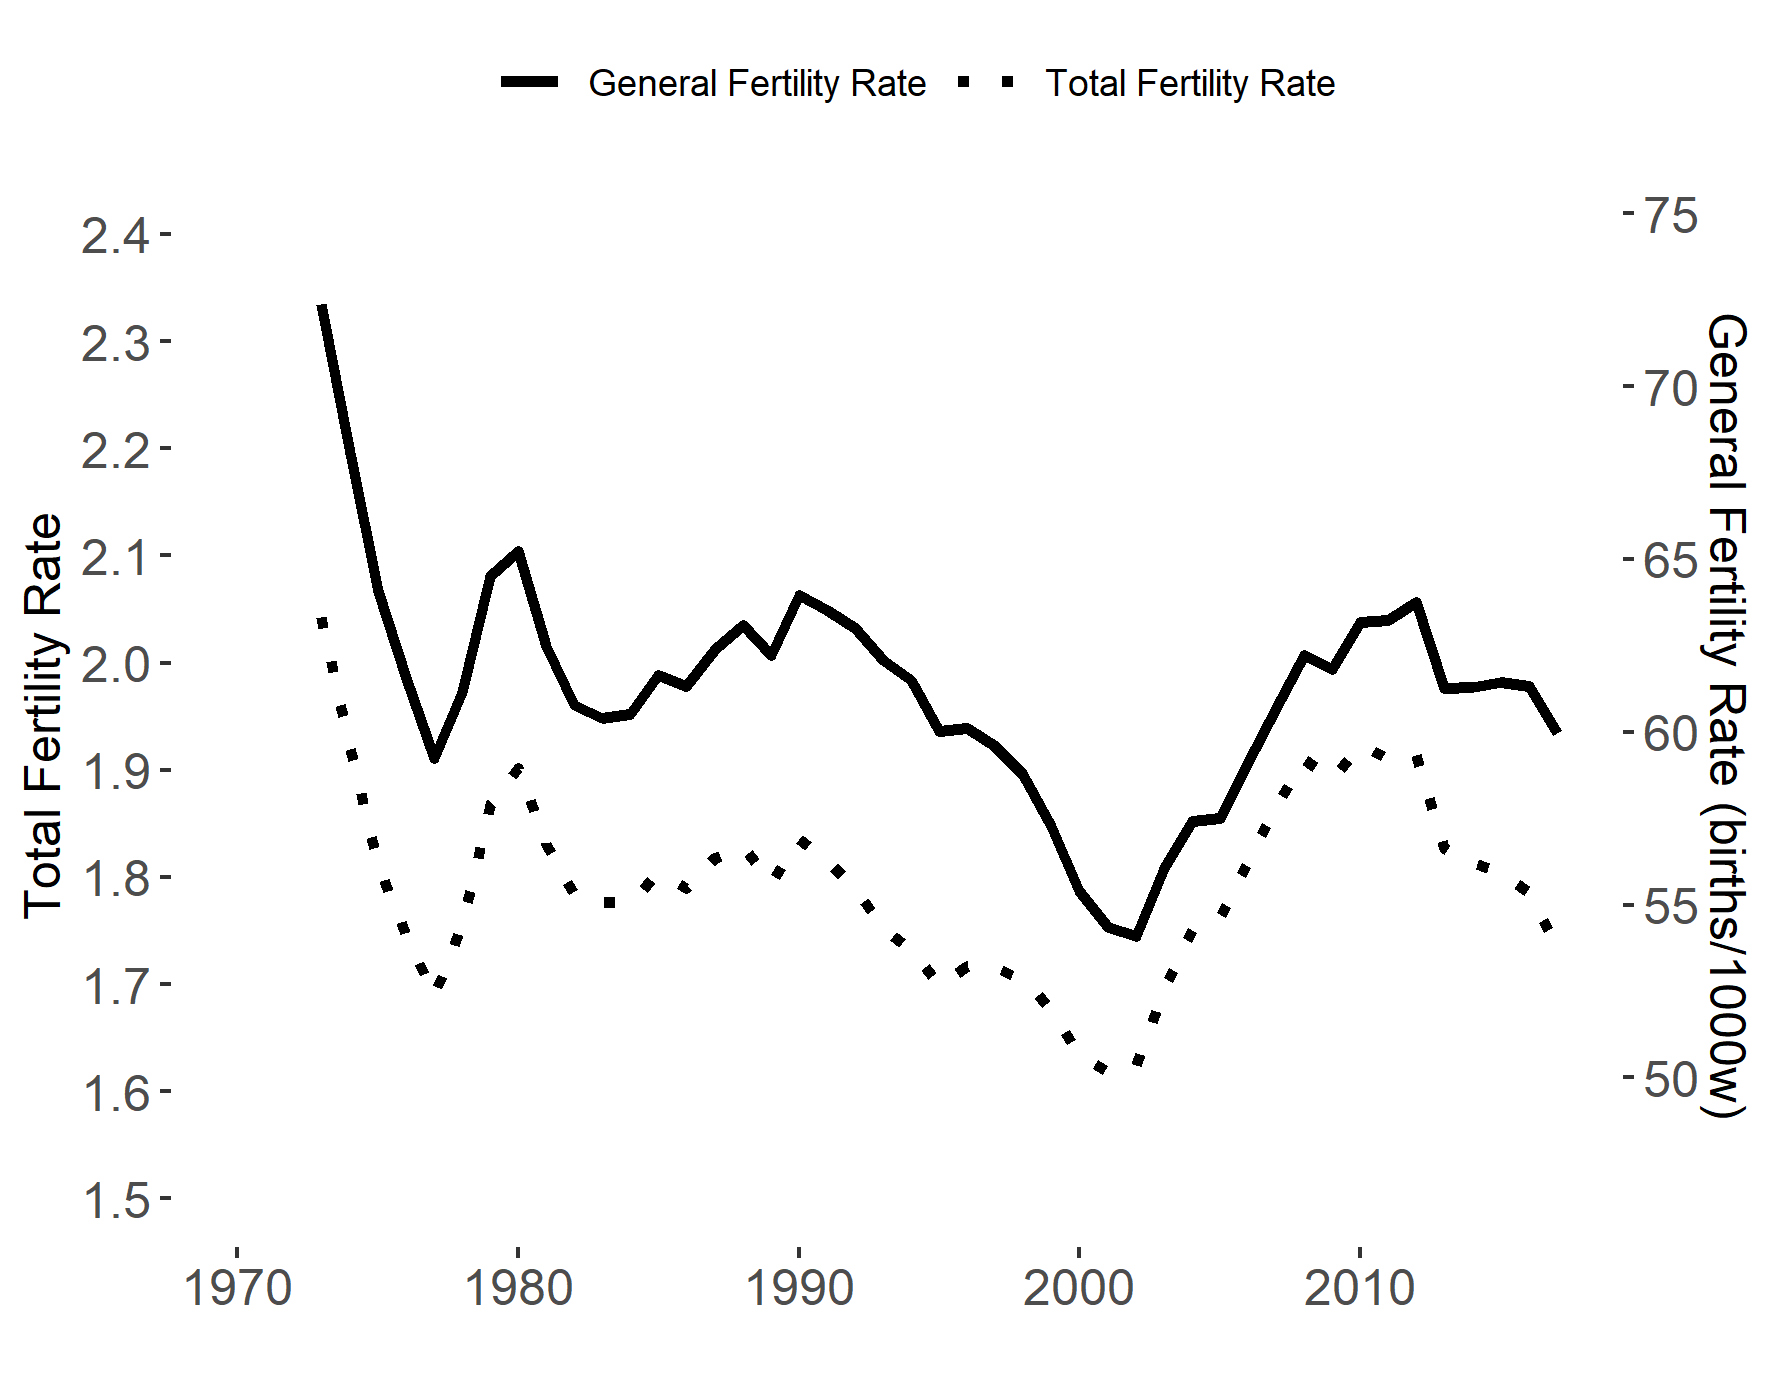
\includegraphics[width=0.7\linewidth]{_resources/chapter_death/fig10} 

}

\caption{Fertility rates for the United Kingdom. Data source: Eurostat. Note: Only births of women aged 15-45 are included.}\label{fig:death1}
\end{figure}

\textbf{What is the chart telling us?}

So why did we combine the two line charts in Figure \ref{fig:death1}? Firstly, the goal was to investigate the link between these two series. The graph is scaled in a way such that the Total Fertility Rate should perfectly overlay the General Fertility Rate if they are the same (that is the level on the right vertical axis is equal to 31 times the corresponding value on the left axis). This is clearly not the case, but we see that the gap narrowed in the early 2000s. This will be the case if the age groups with higher age specific fertility rates are larger. If every age group has the same fertility rate this year and next year, but the number of people in an age group with a relatively high age specific fertility rate is larger next year compared to this year, the General Fertility Rate will increase, but the Total Fertility Rate will be unchanged.

\hypertarget{decomposing-the-development-in-life-births}{%
\subsection{Decomposing the development in life births}\label{decomposing-the-development-in-life-births}}

In the year 2000 the number of life births in England and Wales was 604,441. 16 years later, in 2016, the number of life births was 91,830 higher, at 696,271. What caused caused this increase? We can mechanichally decompose this change into the two underlying factors:

\begin{enumerate}
\def\labelenumi{\arabic{enumi}.}
\tightlist
\item
  The number of women in England and Wales in childbearing age.
\item
  The General Fertility Rate.
\end{enumerate}

It could be the case that the number of life births increased because there are more women in childbearing ages. The fertility behaviour of these women was actually unchanged (in other words, the General Fertility Rate was constant). It could also be the case that the number of women in childbearing age stayed constant, but that the General Fertility Rate increased. Or it could be a mixture of both.

We can use the following formula to decompose the change in life births. Let \(\Delta X\) be the change in life births. We can then write this change as:

\begin{align}
    \Delta X&=Y_1\frac{X_1}{Y_1}-Y_0\frac{X_0}{Y_0}\nonumber\\
\Rightarrow &=\overbrace{Y_0\left(\frac{X_1}{Y_1}-\frac{X_0}{Y_0}\right)}^{A}+\overbrace{\left(Y_1-Y_0\right)\frac{X_0}{Y_0}}^{B}+
    \overbrace{\left(\frac{X_1}{Y_1}-\frac{X_0}{Y_0}\right)\left(Y_1-Y_0\right)}^{C}
\end{align}

Where General Fertility Rate (GFR) the ratio \(X/Y\) and the number of women in childbearing age is \(Y\). Term \(A\) in the forumal above captures the change in life births that is due to the change in General Fertility Rate. \(B\) captures the change that is due to a change in the number of women, and \(C\) captures a combined effect of these changes.

\begin{longtable}[]{@{}llll@{}}
\caption{\label{tab:deathtx} Life births, women in childbearing age and GFR. For England and Wales. Data source: UK Office for National Statistics Birth Summary Tables, England and Wales.}\tabularnewline
\toprule
Year & Life births (\(X\)) & Women aged 15-44 (\(Y\)) & General Fertility Rate (\(X/Y\))\tabularnewline
\midrule
\endfirsthead
\toprule
Year & Life births (\(X\)) & Women aged 15-44 (\(Y\)) & General Fertility Rate (\(X/Y\))\tabularnewline
\midrule
\endhead
2000 & 604,441 & 10,812,898 & 0.0559\tabularnewline
2016 & 696,271 & 11,176,100 & 0.0623\tabularnewline
Change & 91,830 & 363,201 & 0.0064\tabularnewline
\bottomrule
\end{longtable}

Using these numbers in the formula above, we get:

\begin{itemize}
\tightlist
\item
  \(A\) Change in fertility times number of women in 2000: 69,203.
\item
  \(B\) Change in the number of women times fertility in 2000: 20,303.
\item
  \(C\) Combined effect: 2,324.
\item
  Total change: \(A+B+C= 91,830\)
\end{itemize}

The decomposition shows that the change in the number of life birts is mainly due to an increasing General Fertility Rate, the change in the number of women in childbearing age has, however, also contributed positive to the increase.

\hypertarget{life-expectancy}{%
\section{Life expectancy}\label{life-expectancy}}

Having discussed one element of natural population change, births, we now turn to the other aspect: deaths. We will here briefly summarize the construction of life tables and estimation of life expectancy. Life expectancy is often considered one of the most important measures of social progress and it is often used in the public debate, as shown in the example from The Economist in Figure \ref{fig:life}. The tearm "Life expectancy seems quite intuitive. It answers an important question: how long can we expect to life?. But how is it calculated?

\begin{figure}

{\centering 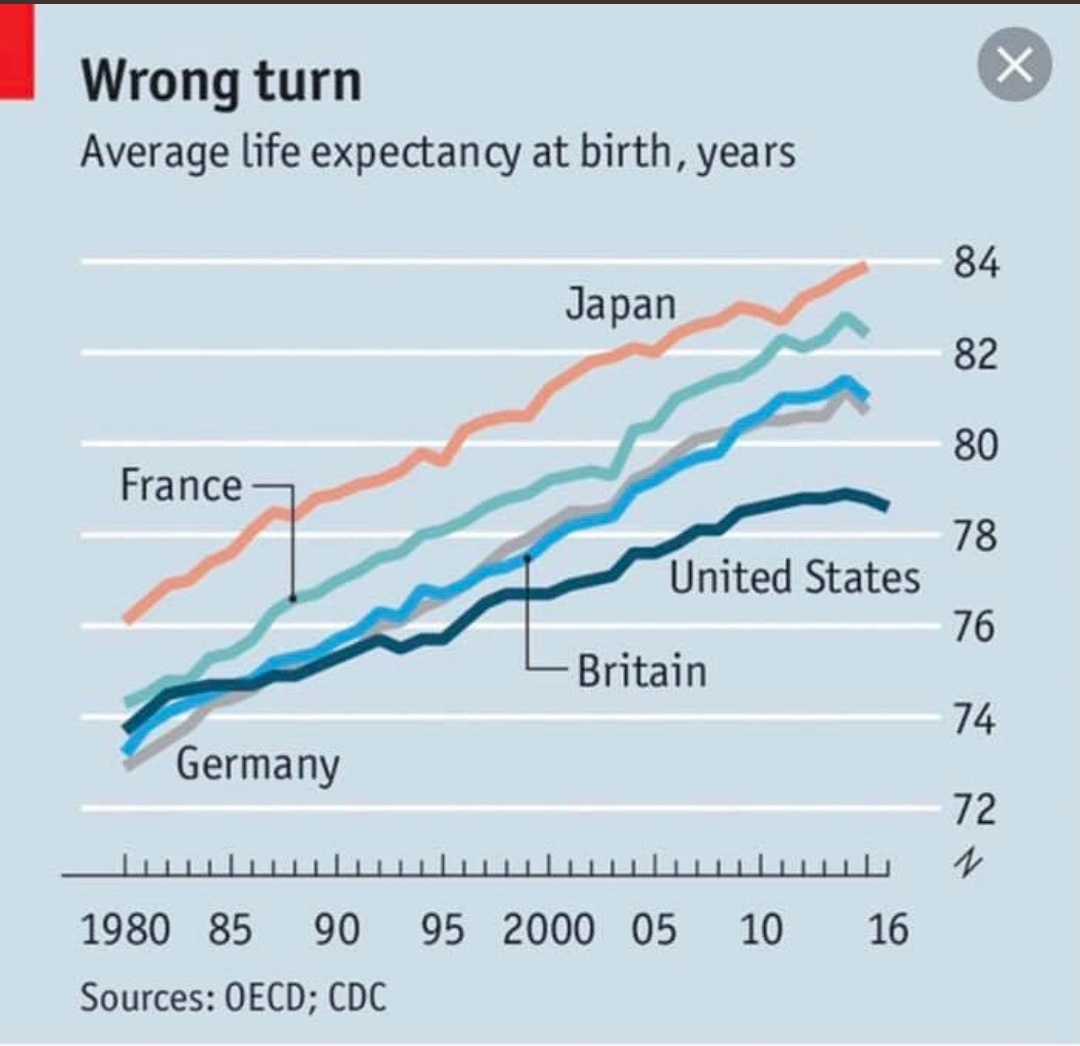
\includegraphics[width=0.5\linewidth]{_resources/chapter_death/economist} 

}

\caption{Example: Comparing the life expectancy across couuntry. Source: The Economist.}\label{fig:life}
\end{figure}

Life tables provide a list of period live expectancies for given age groups. Given you are in a specific age group today and given the mortality rates of each age group, what is your expected life expectancy. The alternative measure, the cohort life expectancy, takes variation in mortality rates across cohorts into account. We will here only cover the period life expectancy and how to construct a life table. It is also one of the most common measures of life expectancy.

The intuition behind the period life expectancy is very similar to the intuition behind the total fertility rate. We simply consider the mortality rate of each age group today, and ask how long we would life. However, because we only can die once, it is slightly more complicated (we can have more children). We therefore first create a life table. Table \ref{tab:deatht} shows the data requirements for creating life tables.

\begin{longtable}[]{@{}llll@{}}
\caption{\label{tab:deatht} Data requirements for life tables}\tabularnewline
\toprule
\begin{minipage}[b]{0.12\columnwidth}\raggedright
Col\strut
\end{minipage} & \begin{minipage}[b]{0.22\columnwidth}\raggedright
Notation\strut
\end{minipage} & \begin{minipage}[b]{0.44\columnwidth}\raggedright
Content\strut
\end{minipage} & \begin{minipage}[b]{0.10\columnwidth}\raggedright
Source\strut
\end{minipage}\tabularnewline
\midrule
\endfirsthead
\toprule
\begin{minipage}[b]{0.12\columnwidth}\raggedright
Col\strut
\end{minipage} & \begin{minipage}[b]{0.22\columnwidth}\raggedright
Notation\strut
\end{minipage} & \begin{minipage}[b]{0.44\columnwidth}\raggedright
Content\strut
\end{minipage} & \begin{minipage}[b]{0.10\columnwidth}\raggedright
Source\strut
\end{minipage}\tabularnewline
\midrule
\endhead
\begin{minipage}[t]{0.12\columnwidth}\raggedright
(1)\strut
\end{minipage} & \begin{minipage}[t]{0.22\columnwidth}\raggedright
\(x,x+n\)\strut
\end{minipage} & \begin{minipage}[t]{0.44\columnwidth}\raggedright
The age interval\strut
\end{minipage} & \begin{minipage}[t]{0.10\columnwidth}\raggedright
Provided\strut
\end{minipage}\tabularnewline
\begin{minipage}[t]{0.12\columnwidth}\raggedright
(2)\strut
\end{minipage} & \begin{minipage}[t]{0.22\columnwidth}\raggedright
\(m_x\)\strut
\end{minipage} & \begin{minipage}[t]{0.44\columnwidth}\raggedright
The age-specific death rate.\strut
\end{minipage} & \begin{minipage}[t]{0.10\columnwidth}\raggedright
\(\frac{\text{deaths } x,x+n}{\text{population } x,x+n }\)\strut
\end{minipage}\tabularnewline
\begin{minipage}[t]{0.12\columnwidth}\raggedright
(3)\strut
\end{minipage} & \begin{minipage}[t]{0.22\columnwidth}\raggedright
\(_nq_n\)\strut
\end{minipage} & \begin{minipage}[t]{0.44\columnwidth}\raggedright
Prob. dying within interval.\strut
\end{minipage} & \begin{minipage}[t]{0.10\columnwidth}\raggedright
\(\frac{2\times n\times m_x}{2+n\times m_x}\)\strut
\end{minipage}\tabularnewline
\begin{minipage}[t]{0.12\columnwidth}\raggedright
(4)\strut
\end{minipage} & \begin{minipage}[t]{0.22\columnwidth}\raggedright
\(I_x\)\strut
\end{minipage} & \begin{minipage}[t]{0.44\columnwidth}\raggedright
Alive at age \(x\)\strut
\end{minipage} & \begin{minipage}[t]{0.10\columnwidth}\raggedright
\(I_0=100,000\)\strut
\end{minipage}\tabularnewline
\begin{minipage}[t]{0.12\columnwidth}\raggedright
\strut
\end{minipage} & \begin{minipage}[t]{0.22\columnwidth}\raggedright
\strut
\end{minipage} & \begin{minipage}[t]{0.44\columnwidth}\raggedright
\strut
\end{minipage} & \begin{minipage}[t]{0.10\columnwidth}\raggedright
\(I_{x+n}=I_x-_nd_x\)\strut
\end{minipage}\tabularnewline
\begin{minipage}[t]{0.12\columnwidth}\raggedright
(5)\strut
\end{minipage} & \begin{minipage}[t]{0.22\columnwidth}\raggedright
\(_nd_x\)\strut
\end{minipage} & \begin{minipage}[t]{0.44\columnwidth}\raggedright
Number of people who die within interval.\strut
\end{minipage} & \begin{minipage}[t]{0.10\columnwidth}\raggedright
\(I_x \times _nq_x\)\strut
\end{minipage}\tabularnewline
\begin{minipage}[t]{0.12\columnwidth}\raggedright
(6)\strut
\end{minipage} & \begin{minipage}[t]{0.22\columnwidth}\raggedright
\(L_x\)\strut
\end{minipage} & \begin{minipage}[t]{0.44\columnwidth}\raggedright
Person-years of life in interval\strut
\end{minipage} & \begin{minipage}[t]{0.10\columnwidth}\raggedright
\(\frac{I_{x}+I_{x+n}}{2}\)\strut
\end{minipage}\tabularnewline
\begin{minipage}[t]{0.12\columnwidth}\raggedright
(7)\strut
\end{minipage} & \begin{minipage}[t]{0.22\columnwidth}\raggedright
\(T_x\)\strut
\end{minipage} & \begin{minipage}[t]{0.44\columnwidth}\raggedright
Cumulative person-years of life\strut
\end{minipage} & \begin{minipage}[t]{0.10\columnwidth}\raggedright
\(\sum_{end}^x{L_x}\)\strut
\end{minipage}\tabularnewline
\begin{minipage}[t]{0.12\columnwidth}\raggedright
(8)\strut
\end{minipage} & \begin{minipage}[t]{0.22\columnwidth}\raggedright
\(e_x\)\strut
\end{minipage} & \begin{minipage}[t]{0.44\columnwidth}\raggedright
Average years of life remaining at age \(x\)\strut
\end{minipage} & \begin{minipage}[t]{0.10\columnwidth}\raggedright
\(T_x/I_x\)\strut
\end{minipage}\tabularnewline
\bottomrule
\end{longtable}

For each age group we require data on the number of people in that group and the number of people who died in that group. Once we have these two variables we can construct the other variables. The first variable we construct is the age specific death rate, following by the probability of dying within the age group interval. We then construct a synthetic population that has a size of 100,000 individuals at the beginning of the first period. In each period we calculate the number of people who survive to this period and who die within this period. We can then use these estimates to calculate the number of life years lived in this period, and sum over these live years. At the end, we divide the number of life years left in any given period by the number of people getting to this period to obtain the estimated life expectancy.

\begin{longtable}[]{@{}llllllll@{}}
\caption{\label{tab:deatht2} Life table for the United Kingdom. Data source: Eurostat.}\tabularnewline
\toprule
age & mx & nqx & ndx & Ix & Lx & Tx & ex\tabularnewline
\midrule
\endfirsthead
\toprule
age & mx & nqx & ndx & Ix & Lx & Tx & ex\tabularnewline
\midrule
\endhead
0 & 0.004 & 0.004 & 385.000 & 100,000 & 99,808 & 8,081,572 & 80.816\tabularnewline
1 & 0.000 & 0.000 & 25.376 & 99,615 & 99,602 & 7,981,765 & 80.126\tabularnewline
2 & 0.000 & 0.000 & 14.013 & 99,589 & 99,582 & 7,882,163 & 79.147\tabularnewline
3 & 0.000 & 0.000 & 11.453 & 99,574 & 99,568 & 7,782,581 & 78.159\tabularnewline
\ldots{} & \ldots{} & \ldots{} & \ldots{} & \ldots{} & \ldots{} & \ldots{} & \ldots{}\tabularnewline
98 & 0.346 & 0.295 & 980.052 & 3326 & 2836 & 3128 & 0.941\tabularnewline
99 & 0.386 & 0.324 & 758.769 & 2345 & 293 & 293 & 0.125\tabularnewline
\bottomrule
\end{longtable}

Table \ref{tab:deatht} shows a subset of a life table for the United Kingdom using data from Eurostat and the recipe outlined in Table \ref{tab:deatht2}. Figure \ref{fig:death2} shows a graph of the live expectancy (the last column of Table \ref{tab:deatht2}) and survival rate for the United Kingdom based on data from Eurostat.

\begin{figure}

{\centering 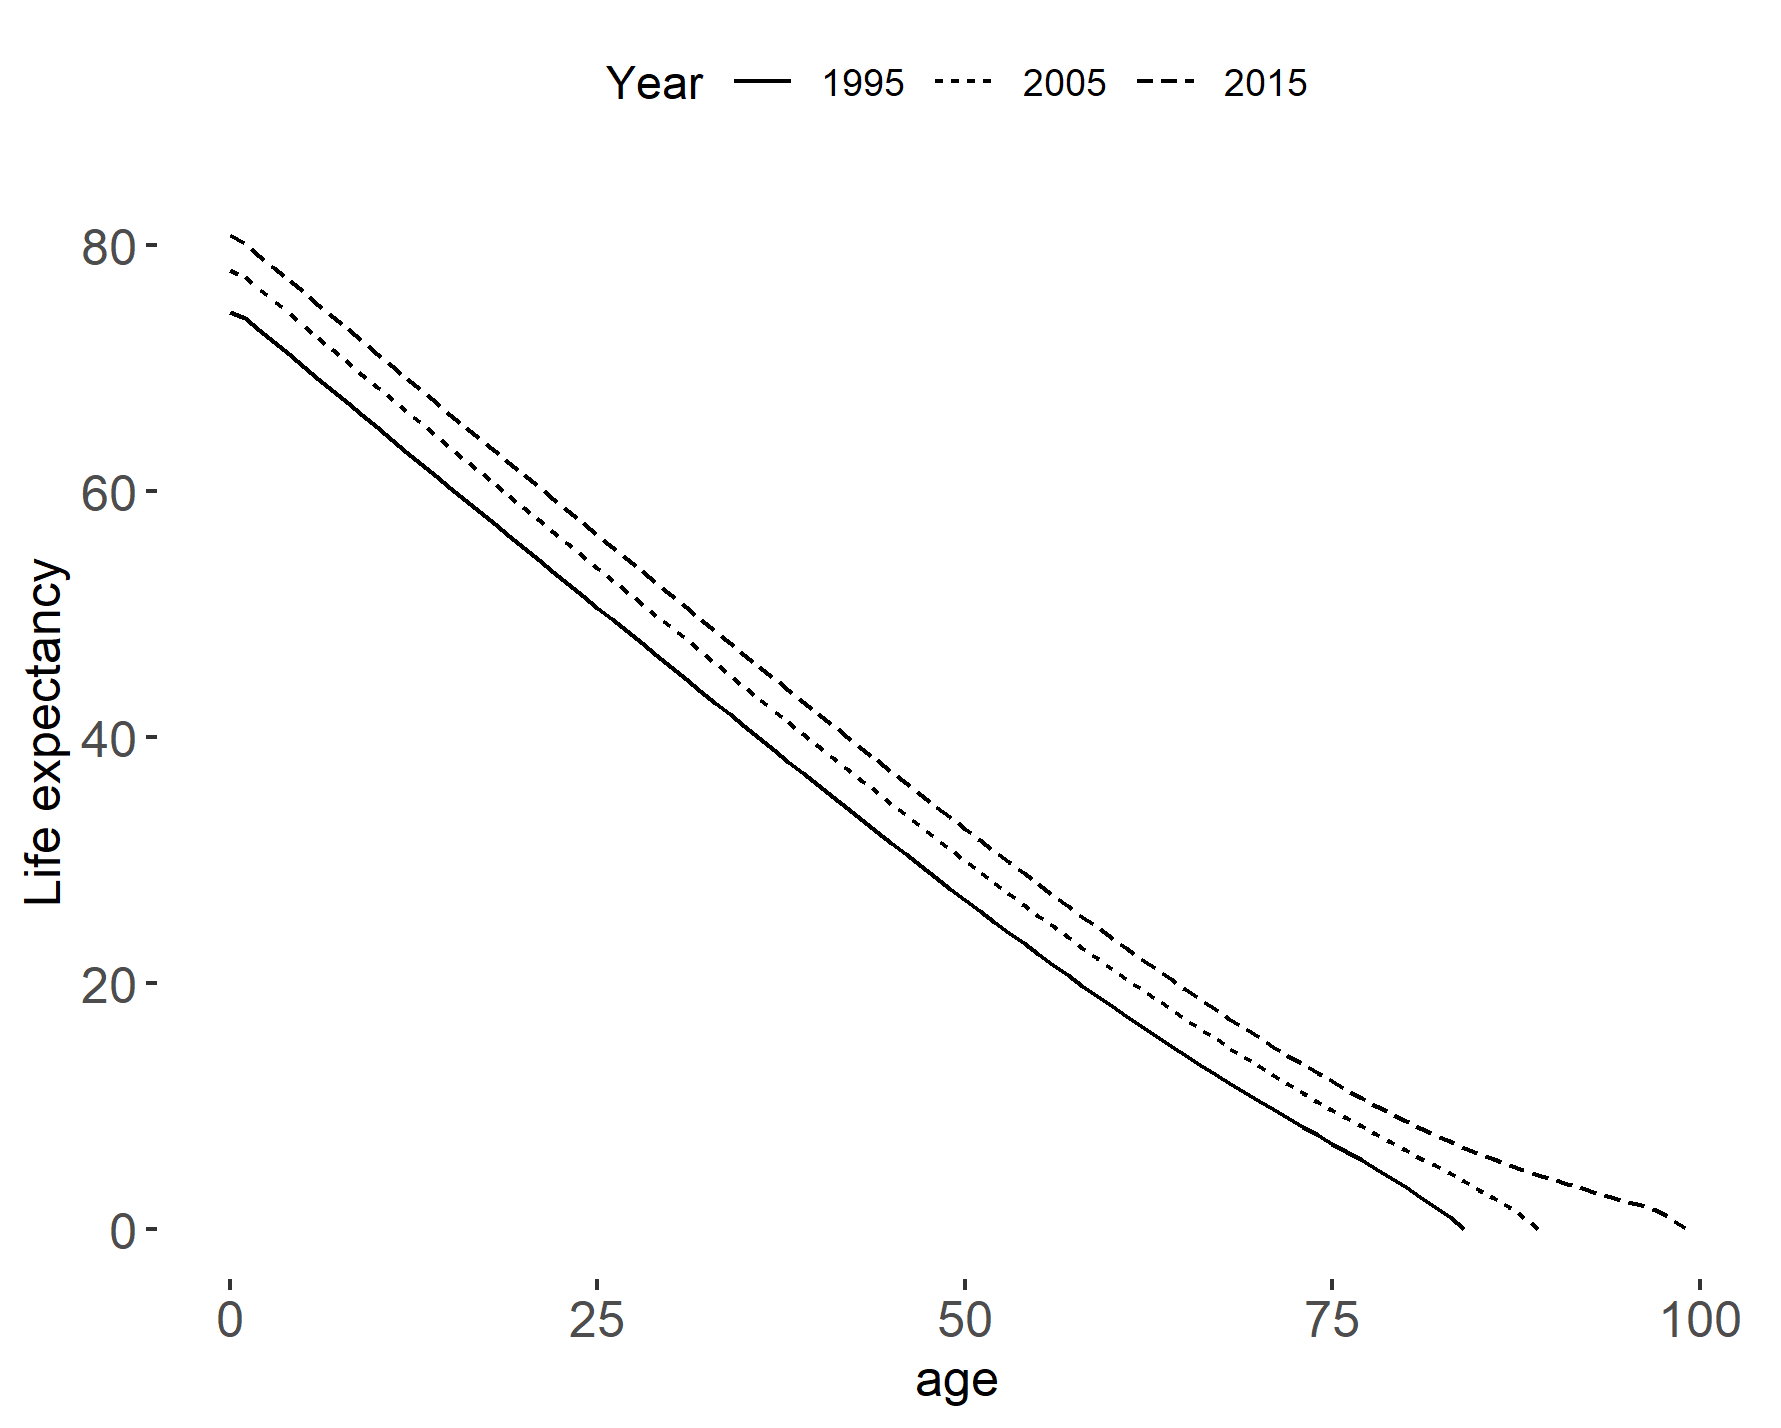
\includegraphics[width=0.5\linewidth]{_resources/chapter_death/fig11} 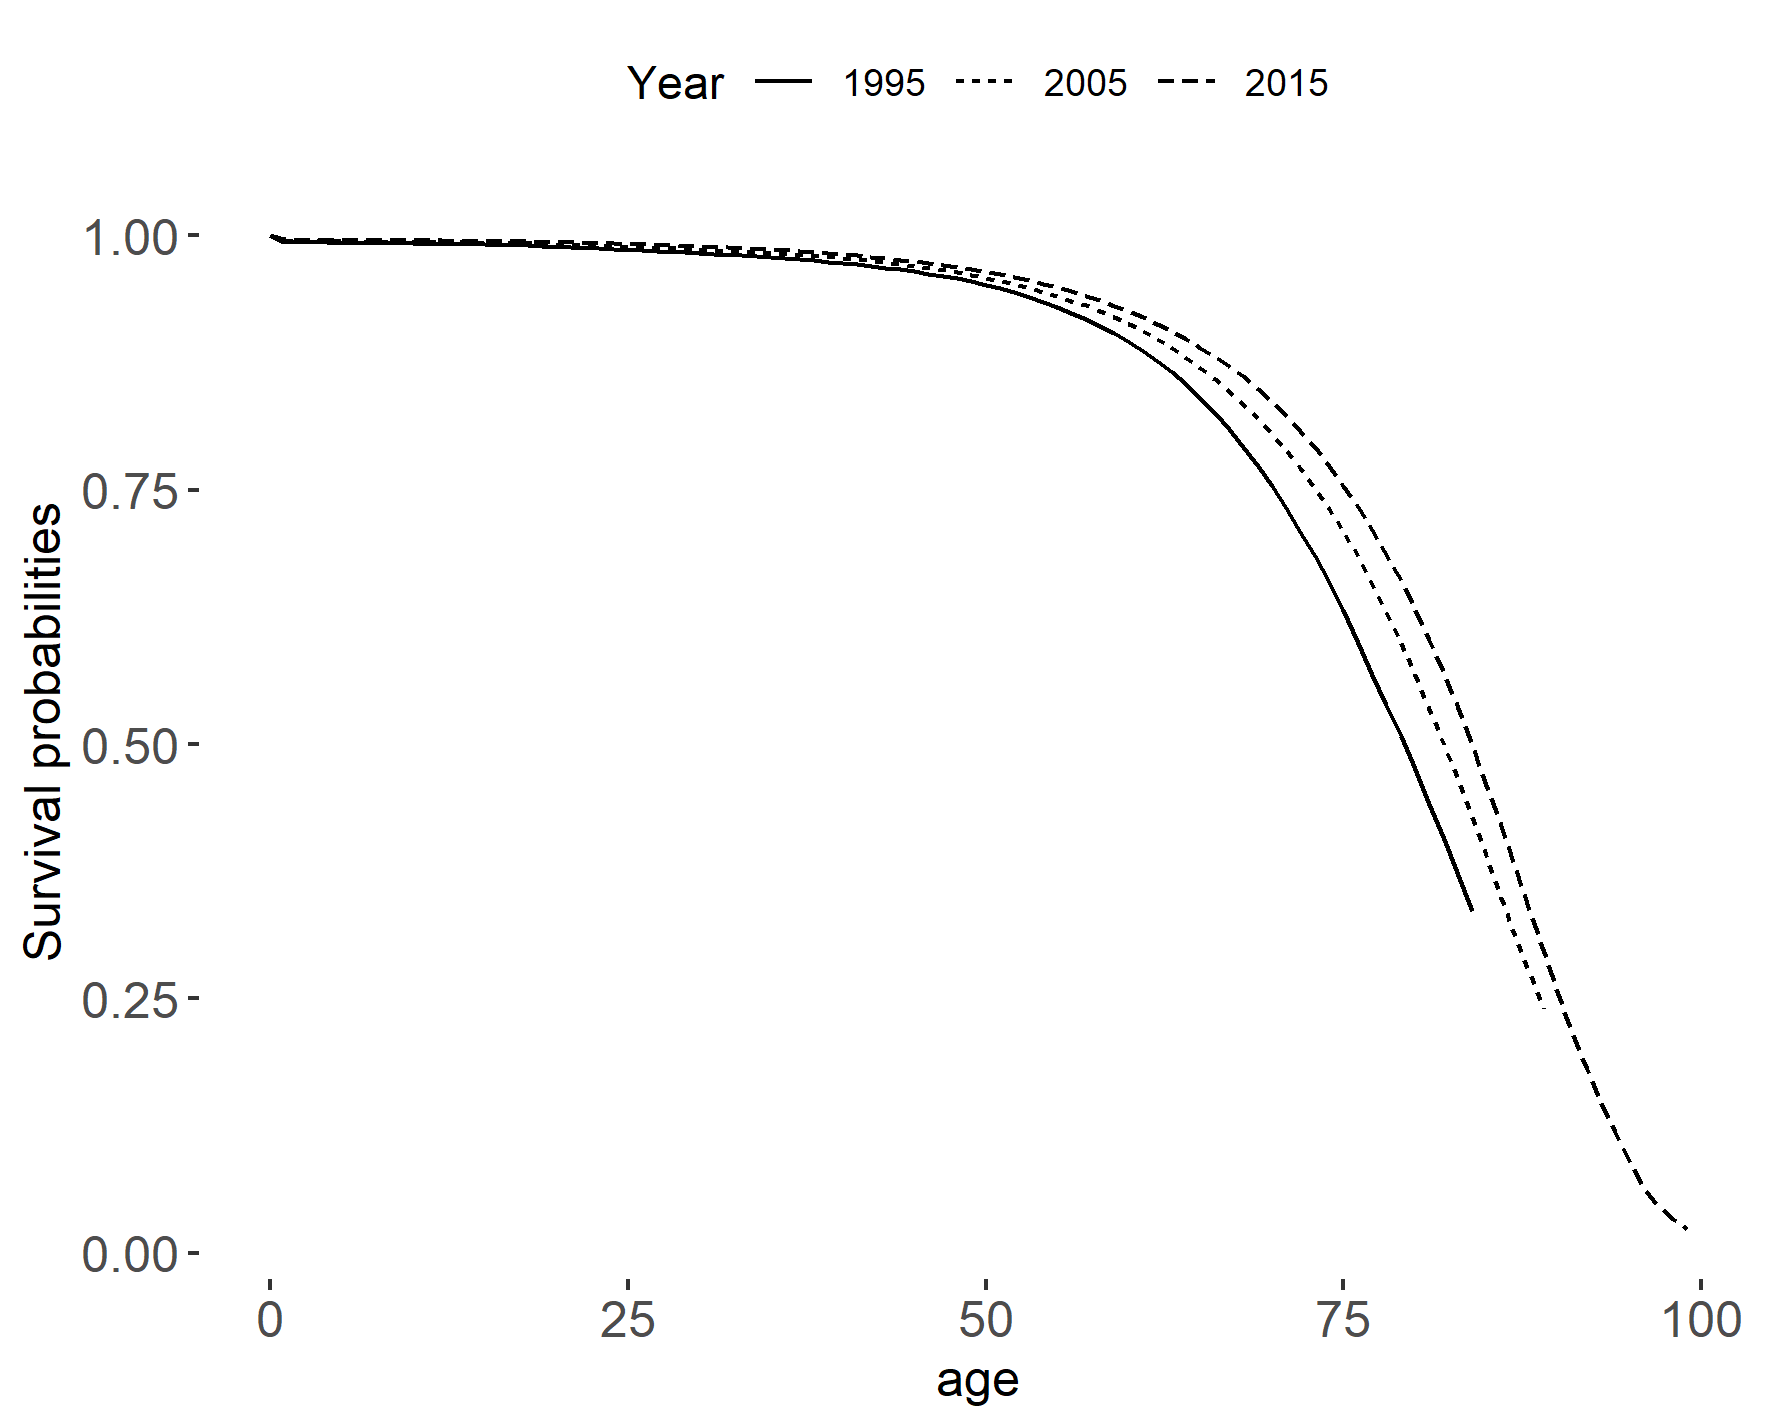
\includegraphics[width=0.5\linewidth]{_resources/chapter_death/fig12} 

}

\caption{Life expectancy by age (left) and survival probabilities (right). Data source: Eurostat. }\label{fig:death2}
\end{figure}

\hypertarget{summary-2}{%
\section{Summary}\label{summary-2}}

So what should you take away from this chapter?

\begin{itemize}
\tightlist
\item
  Measures of fertility

  \begin{itemize}
  \tightlist
  \item
    The Age-Specific Fertility Rate
  \item
    The Total Fertility Rate
  \item
    The General Fertility Rate
  \item
    The Crude Birth Rate
  \end{itemize}
\item
  Decompose changes in life births.
\item
  Creating life tables
\item
  Calculating life expectancy
\end{itemize}

\hypertarget{prices}{%
\chapter{Prices}\label{prices}}

\hypertarget{about-this-chapter-3}{%
\section{About this chapter}\label{about-this-chapter-3}}

We've we discussed how the Policy Interest Rate is set by the Bank of England. The Bank of England has one objective in mind when deciding on the interest rate, the inflation in the UK should be 2 percent. So if you had spend 100 GBP to buy a basket of goods last year, you should spend 102 GBP to buy the basket of goods this year, that gives you the same utility. If the price of the basket is now less than 101 or more than 103 the Bank of England is required to explain why. In other words, the Bank of England faces an inflation target of 2 percent, and deviations of more than one percentage point requires a public explanation. Now this all sounds simple and straightforward. However, the question is what baskets of goods should we compare? Should the basket this year contain exactly the same goods as the basket last year, in the same quantity and quality? What if a new product arrives on the market? We will discuss these issues in this lecture along with the concept of the Purchasing Power Parity, which concerns the comparison of prices across countries.

\hypertarget{intended-learning-outcomes-3}{%
\subsection{Intended learning outcomes}\label{intended-learning-outcomes-3}}

After this lecture you should be able to

\begin{itemize}
\tightlist
\item
  Explain the difference between the Laspeyre and Paasche price index.
\item
  Explain how the consumer price index is constructed.
\item
  Explain what inflation is and how it is measured.
\item
  Explain what Purchasing Power Parity is, and how we can use it to compare prices across countries.
\end{itemize}

\hypertarget{price-indexes---in-theory}{%
\section{Price indexes - in theory}\label{price-indexes---in-theory}}

\hypertarget{the-objective}{%
\subsection{The objective}\label{the-objective}}

Before we discuss how we measure changes in prices, let's briefly discuss what our objective is. There are many different price indexes, such as the consumer price index, the producer price index, the house price index and the GDP deflator. They all track the development of prices, but they focus on the prices of slightly different goods. The consumer price index, which is the index central banks typically use in the inflation target, measures the development of prices over time. We would like to know, as a consumer, how much more expensive (in nominal terms) is it today compared to yesterday. But what comparison should we make? There are many goods and prices, and we need to combine their development in one overall number. We therefore compare the price of a basket of good over time. And what determines the composition of this basket? A fair comparison would be to compare two baskets that gives us the same utility. Unfortunately we do not observe people's utility, and it is therefore not possible to make this comparison in practice. The price indexes discussed in the next section are therefore concerned in how we in practice can crate this basket of goods.

\hypertarget{a-simple-index}{%
\subsection{A simple index}\label{a-simple-index}}

Let us first revisit the index concept we used in the first week. We constructed indexes separately for each variable. In other words, for each variable, there is one index:

\begin{align}
    I_t=100\times \frac{P_t}{P_0}
    \label{eq1}
\end{align}

Where \(I_t\) is the index value of price \(P\) at time \(t\), using time \(t=0\) as the base year. Note that we also have that:
\begin{align}
    I_{t-1}=100\times \frac{P_{t-1}}{P_0}
    \label{eq2}
\end{align}

which we can rewrite to:

\begin{align}
    Y_0=100\times \frac{P_{t-1}}{I_{t-1}}
    \label{eq3}
\end{align}

And then insert in equation \eqref{eq1}:

\begin{align}
    I_t&=100\times \frac{P_t}{100\times \frac{P_{t-1}}{I_{t-1}}}\nonumber\\
        \Rightarrow I_t&=I_{t-1}\times \frac{P_t}{ P_{t-1}}\nonumber\\
    \label{eq4}
\end{align}

Instead of computing the index based on base year, we take the index value last period and multiply by the change in our variable from last year to this year. Table \ref{tab:price1} shows a simple example of two indexes based on two time series.

\begin{longtable}[]{@{}ccccc@{}}
\caption{\label{tab:price1} Simple indexes of two prices}\tabularnewline
\toprule
Year & P1 & I(P1) & P2A & I(P2)\tabularnewline
\midrule
\endfirsthead
\toprule
Year & P1 & I(P1) & P2A & I(P2)\tabularnewline
\midrule
\endhead
2001 & 136 & 100 & 120 & 100\tabularnewline
2002 & 186 & 137 & 127 & 106\tabularnewline
2003 & 197 & 145 & 140 & 117\tabularnewline
2004 & 204 & 150 & 138 & 115\tabularnewline
2005 & 215 & 158 & 150 & 125\tabularnewline
2006 & 222 & 163 & 160 & 133\tabularnewline
\bottomrule
\end{longtable}

But what if \(P1\) is the price of coffee and \(P2\) is the price of tea, and we would like to summarize the price development in one index variable? One approach would simply be to take the average across these two products:

\begin{align}
   I_t&=100\times \left(\frac{0.5\times P1_t+0.5\times P2_t}{0.5\times P1_0+0.5\times P2_0}\right)
    \label{eq5}
\end{align}

Which gives us the index shown in Table \ref{tab:price2} . The new single index value is always between the two separate index values in Table \ref{tab:price1}, because the new index is based on the simple mean across these two variables.

\begin{longtable}[]{@{}ccccc@{}}
\caption{\label{tab:price2} Index based on the simple mean across two variables}\tabularnewline
\toprule
Year & P1 & P2 & PA & I(PA)\tabularnewline
\midrule
\endfirsthead
\toprule
Year & P1 & P2 & PA & I(PA)\tabularnewline
\midrule
\endhead
2001 & 136 & 100 & 128.0 & 100\tabularnewline
2002 & 186 & 137 & 156.5 & 122\tabularnewline
2003 & 197 & 145 & 168.5 & 132\tabularnewline
2004 & 204 & 150 & 171.0 & 134\tabularnewline
2005 & 215 & 158 & 182.5 & 143\tabularnewline
2006 & 222 & 163 & 191.0 & 149\tabularnewline
\bottomrule
\end{longtable}

But what if we drink much more coffee than tea (I am not British)? Let's say that for every four cups we drink, three of them are coffee and one of them is tea. Now this should also be reflected in our price index. The simple arithmetic mean is therefore not representative, instead we should use the weighted mean, where we assign tea a weight that is three times higher than coffee:

\begin{align}
   I_t&=100\times \left(\frac{0.75\times P1_t+0.25\times P2_t}{0.75\times P1_0+0.25\times P2_0}\right)
    \label{eq6}
\end{align}

or expressed in more general terms:

\begin{align}
   I_t&=100\times \left(\frac{Q1 \times P1_t+Q2 \times P2_t}{Q1 \times P1_0+Q2 \times P2_0}\right)
    \label{eq7}
\end{align}

Where \(Q\) refers to the quantities or weights.

Table \ref{tab:price3} shows the weighted price index, along with the weights, \(Q\). The overall price of our hot drinks consumption now increased 56 percent from 2001 to 2006, this is slightly higher than the price index in Table \ref{tab:price2}, reflecting that the price of coffee has increased more than tea, and we consume relatively more coffee.

\begin{longtable}[]{@{}ccccc@{}}
\caption{\label{tab:price3} Index based on a weighted mean across two variables. With \(I=0.75 imes P1+0.25 imes P2\).}\tabularnewline
\toprule
Year & P1 & P2 & Q1 & Q2\tabularnewline
\midrule
\endfirsthead
\toprule
Year & P1 & P2 & Q1 & Q2\tabularnewline
\midrule
\endhead
2001 & 136 & 100 & 75 & 25\tabularnewline
2002 & 186 & 137 & 75 & 25\tabularnewline
2003 & 197 & 145 & 75 & 25\tabularnewline
2004 & 204 & 150 & 75 & 25\tabularnewline
2005 & 215 & 158 & 75 & 25\tabularnewline
2006 & 222 & 163 & 75 & 25\tabularnewline
\bottomrule
\end{longtable}

Computing a price index has been quite straightforward so far. However, in the later years we started to drink relatively more tea, so the weights changed. This is where we introduce slightly more complex price indexes.

\hypertarget{the-laspeyre-index}{%
\subsection{The Laspeyre Index}\label{the-laspeyre-index}}

The German economist and Etienne Laspeyre is the father of the Laspeyere index. In terms of our two goods world, with only tea and coffee, Laspeyre's index is defined as:

\begin{align}
I_t^L&=100\times \left(\frac{Q1_0 \times P1_t+Q2_0 \times P2_t}{Q1_0 \times P1_0+Q2_0 \times P2_0}\right)
    \label{eq8}
\end{align}

What is new compared to equation \eqref{eq6} is that not only do the prices have time periods, but also the weights (the quantities), \(Q\). Using Laspeyre's index, the weights are kept constant at the initial period, 0. In other words, Laspeyre's index tells us how much the price of our consumption has increased, given the relative weights in the base year. In more general terms (with more goods), we can write Laspeyre's index as follows:

\begin{align}
   I_t^L&=100\times \left(\frac{\sum^I_{i=1} Qi_0 \times Pi_t}{\sum^I_{i=1}Qi_0 \times Pi_0}\right)
    \label{eq9}
\end{align}

Where \(i\) refers to the product. So in the case of the Laspeyre price index, our movement away from tea to coffee is ignored. If we wanted to adjust the weights, an alternative methodology is provided by Paasche.

\hypertarget{the-paasche-price-index}{%
\subsection{The Paasche Price Index}\label{the-paasche-price-index}}

As with the Laspeyre index, the Paasche index is attributable to a German economist, this time it is Hermann Paasche. The Paasche index is very much just the opposite of the Laspeyre index. We use the current weights, both in the denominator and numerator.

\begin{align}
   I_t^P&=100\times \left(\frac{\sum^I_{i=1} Qi_t \times Pi_t}{\sum^I_{i=1}Qi_t \times Pi_0}\right)
    \label{eq10}
\end{align}

Instead of always comparing the sample basket we bought in the reference period, we refer to the basket, in the current period. Table \ref{tab:price4} shows the Laspeyre index (\(I^L\)) and the Paasche index (\(I^P\)) for our two good case, where the quantities or weights change from year to year. Unsurprisingly, the Laspeyre index corresponds to the weighted average in Table \ref{tab:price3}, because the weight in the base year corresponds to the constant weights in Table \ref{tab:price3} . The Paasche index is, however, slightly different. Going back to Table \ref{tab:price1} we recall that the price of the first good (say coffee) increased more than the price of the second good (say tea). Now as we start consuming relatively more tea, the good that increases less in price receives more weight. The Laspeyre index ignores this, but the Paasche does not, and therefore the Paasche price index is lower than the Laspeyre index.

\begin{longtable}[]{@{}ccccc@{}}
\caption{\label{tab:price4} The Laspeyre and Paasche Index. Notes: \(I^L\) refers to the Laspeyre price index and \(I^P\) refers to the Paasche price index.}\tabularnewline
\toprule
Year & P1 & P2 & Q1 & Q2\tabularnewline
\midrule
\endfirsthead
\toprule
Year & P1 & P2 & Q1 & Q2\tabularnewline
\midrule
\endhead
2001 & 136 & 100 & 75 & 25\tabularnewline
2002 & 186 & 137 & 65 & 35\tabularnewline
2003 & 197 & 145 & 55 & 45\tabularnewline
2004 & 204 & 150 & 45 & 55\tabularnewline
2005 & 215 & 158 & 35 & 65\tabularnewline
2006 & 222 & 163 & 25 & 75\tabularnewline
\bottomrule
\end{longtable}

Our example is actually in line with what we typically observe in the real world, the Laspeyre index gives a higher increase than the Paasche index. This is because consumers tend to substitute away from the good that increases relatively more in price. So when one good's price increases less than the other, and we therefore tend to consumer more of the relatively cheaper good, the Paasche index takes this into account because weights are updated every year. The Laspeyre index on the other hand always refers to the base year weights. Which index to prefer is, however, not obvious. Often the choice of index will be based on practical reasons. While the Paasche index requires new weights every year, the Laspeyre index only requires the base year weights and the prices for all periods. The Paasche index is therefore slightly more data demanding.

\hypertarget{the-fisher-price-index}{%
\subsection{The Fisher Price Index}\label{the-fisher-price-index}}

The Fisher index, introduced by the american economist Irving Fisher, is a compromise between the Laspeyre index and the Paasche index. It is also called Fisher ideal index, and it is based on an average between the Laspeyre and Paasche index. The average is computed by means of a geometric mean:

\begin{align}
      I_t^F&=\sqrt{I^ L_t\times I^ P_t} 
    \label{eq11}
\end{align}

Table \ref{tab:price5} includes the Fisher ideal index. As we would expect (given that the mean), the the Fisher ideal index is always between the Laspeyre and the Paasche index.

\begin{longtable}[]{@{}ccccc@{}}
\caption{\label{tab:price5} The Laspeyre, Paasche and Fisher Ideal Index. Notes: \(I^L\) refers to the Laspeyre price index, \(I^P\) refers to the Paasche price index and \(I^F\) refers to the Fisher ideal price index.}\tabularnewline
\toprule
Year & P1 & P2 & Q1 & Q2\tabularnewline
\midrule
\endfirsthead
\toprule
Year & P1 & P2 & Q1 & Q2\tabularnewline
\midrule
\endhead
2001 & 136 & 100 & 75 & 25\tabularnewline
2002 & 186 & 137 & 65 & 35\tabularnewline
2003 & 197 & 145 & 55 & 45\tabularnewline
2004 & 204 & 150 & 45 & 55\tabularnewline
2005 & 215 & 158 & 35 & 65\tabularnewline
2006 & 222 & 163 & 25 & 75\tabularnewline
\bottomrule
\end{longtable}

\hypertarget{the-lowe-price-index}{%
\subsection{The Lowe Price Index}\label{the-lowe-price-index}}

The Lowe price index is attributed to the Scottish economist Joseph Lowe. The Lowe index is a more general price index, where the reference period for the weights is not set.

\begin{align}
   I_t^{Lo}&=100\times \left(\frac{\sum^I_{i=1} Qi_r \times Pi_t}{\sum^I_{i=1}Qi_r \times Pi_0}\right)
    \label{eq12}
\end{align}

The Laspeyre price index is a special case of the Lowe price index, where \(r=0\), and the Paasche price index is a special case of the the Lowe price index, where \(r=t\). The Laspeyre and the Paasche indexes are therefore often called ``Lowe type price indexes''.

\hypertarget{other-indexes}{%
\subsection{Other indexes}\label{other-indexes}}

There are many different price indexes, and the price indexes applied by statistical offices will often be modified versions of the standard formulas. One modification is chain-linking, which we will discuss in the next section. However, before we get there, it is worth mentioning a few more price indexes. The Finnish statistician Leo Törnqvist introduced an index (the Törnqvist index), where we instead of taking the mean between the Fisher and Paasche index, take the mean of the weights between the base year and the current year. However, the Törnqvist index also differs by using a weighted geometric mean instead of the weighted arithmetic mean.

Also, another index worth mentioning is the Carli index, introduced by the Italian economist Gian Carli:

\begin{align}
   I_t^{C}&=\frac{1}{N}\sum^I_{i=1}\left(\frac{Pi_t}{Pi_0}\right)
    \label{eq13}
\end{align}

Note that the Carli index is unweighed. It is therefore called elementary, and it is typically only used when we are focusing on specific product types.

\hypertarget{chain-linked-vs.-unchained-indexes}{%
\subsection{Chain-linked vs.~unchained indexes}\label{chain-linked-vs.-unchained-indexes}}

So far we've three solutions regarding product weights. One, we use the weights in the base year (Laspeyre); two, we use the weights in the current year (Paasche); three we use an average between the base year and the current year (Fisher/Tornqvist). An alternative strategy is to constantly update the base year of the weights. This is where the alternative specification in equation \eqref{eq4} becomes handy. Recall that the we could write the price index in year \(t\) as the price index in year \(t-1\) times the change from year \(t-1\) to \(t\). In general terms, as a chain-linked Laspeyere index, this works as follows:

\begin{align}
   I_t^{CL}&=I_{t-1}\times  \left(\frac{\sum^I_{i=1} Qi_{t-1} \times Pi_t}{\sum^I_{i=1}Qi_{t-1} \times Pi_{t-1}}\right)
\end{align}

We call this methodology for chained, because we link each year using a chain of updated weights. We thus use the standard Laspeyre index, but every year we update the base year as the last year. We can do a similar exercise with the Paasche index

\begin{align}
   I_t^{CP}&=I_{t-1}\times  \left(\frac{\sum^I_{i=1} Qi_{t} \times Pi_t}{\sum^I_{i=1}Qi_{t} \times Pi_{t-1}}\right)
\end{align}

\begin{longtable}[]{@{}ccccc@{}}
\caption{\label{tab:price6} Laspeyre and Paasche index, unchained and chain-linked. Notes: \(I^L\) refers to the Laspeyre price index, \(I^P\) refers to the Paasche price index, \(I^{CL}\) refers to the chain-linked Laspeyre index and \(I^{CP}\) to the chain-linked Paasche index.}\tabularnewline
\toprule
Year & P1 & P2 & Q1 & Q2\tabularnewline
\midrule
\endfirsthead
\toprule
Year & P1 & P2 & Q1 & Q2\tabularnewline
\midrule
\endhead
2001 & 136 & 100 & 75 & 25\tabularnewline
2002 & 186 & 137 & 65 & 35\tabularnewline
2003 & 197 & 145 & 55 & 45\tabularnewline
2004 & 204 & 150 & 45 & 55\tabularnewline
2005 & 215 & 158 & 35 & 65\tabularnewline
2006 & 222 & 163 & 25 & 75\tabularnewline
\bottomrule
\end{longtable}

\hypertarget{summary-on-price-indexes}{%
\subsection{Summary on price indexes}\label{summary-on-price-indexes}}

\emph{Objective}

\begin{itemize}
\tightlist
\item
  A method to compare the price development across a large bundle of goods.
\end{itemize}

\emph{Challenge}

\begin{itemize}
\tightlist
\item
  The composition of the bundle might change over time, and some goods might gain higher and lower weight, while other goods might be removed or added to the bundle.
\end{itemize}

\emph{Method}

\begin{itemize}
\tightlist
\item
  The Laspeyre index: Keep the bundle fixed in the base year and assess the price development based on the development of the costs of the initial bundle.
\item
  The Paasche index: Update the bundle every year, and compare the price of the new bundle given current prices and given prices in the base year.
\item
  The Fisher index: The geometric mean of the Laspeyre and the Paasche indexes.
\item
  Chain-linking: Continuously update the reference period.
\end{itemize}

\hypertarget{weigths}{%
\subsection{Weigths}\label{weigths}}

Before we turn to the actual price indexes, we will briefly discuss how these weights are computed, \(Q1\) and \(Q2\). These weights could be obtained by various sources. In practice, most countries compute the weights based on total household final expenditure from the national accounts.

However, some indexes use surveys to compute the weights. For the UK, the Living Costs and Food Survey is based on reported consumption over a two week period for thousands of households. This survey is used in some price indexes constructed by the ONS (for example the RPI). One advantage of using surveys to compute weights is that we have more information on the household, and we can thus rely on households that we believe are more representative.

\hypertarget{price-indexes---in-practice}{%
\section{Price indexes - in practice}\label{price-indexes---in-practice}}

There is not only one price index. We might for example be interest in how costs for firms have developed. The typical consumption basket for firms is very likely to be different than the typical basket for households.

\hypertarget{consumer-price-indexes}{%
\subsection{Consumer Price Indexes}\label{consumer-price-indexes}}

Let us first consider how the price level for consumers develops. The ONS publishes several consumer price indexes. Let us consider three of the most important ones:

\begin{itemize}
\tightlist
\item
  The Consumer Price Index (CPI)
\item
  The Consumer Prices Index including owner occupiers' housing costs (CPIH)
\item
  The Retail Prices Index (RPI)
\end{itemize}

The CPI is calculated in line with European regulations, but the RPI does not satisfy the international standard. The latter is therefore not regarded as a National Statistic of the ONS any more, but it is still produced, because contracts still rely on the RPI. The main difference between the CPI and the CPIH is that the CPIH includes costs related to owning a home, such as maintenance (owner occupiers' housing costs). The CPI and CPIH include the same items, except for the housing costs. The RPI differs somewhat to the CPI and CPIH in terms of items included. While the weights in the CPI and CPIH are based on total household final expenditure from the national accounts, the weights in the RPI are based on the Living Costs and Food Survey. The CPI is based on about 180,000 prices that cover about 700 items.

The CPI and CPIH are chain-linked Laspeyres-type price indexes computed on a monthly basis. The RPI is (approximately) also a chain-linked Laspeyre type index, but based on annual data.

Looking beyond the UK, the harmonised index of consumer prices (HICP), is the consumer price index by the European Union/ Eurostat, which is also a chain-linked Laspeyres-type price index. Both the CPI and CPIH use weights that are typically updated annually. For more details on the consumer price indexes, see \citep{cpions} for the ONS and \citep{cpieu} for the European level.

There are various data sources for price indexes. Figure \ref{fig:pricefig1} uses data from Eurostat to show the development in the price index for the UK and for the EURO area as a whole. Note that the index is based on 2015 as a reference year. This is slightly unusual, as we often prefer to have the first period as a reference.

\begin{figure}

{\centering 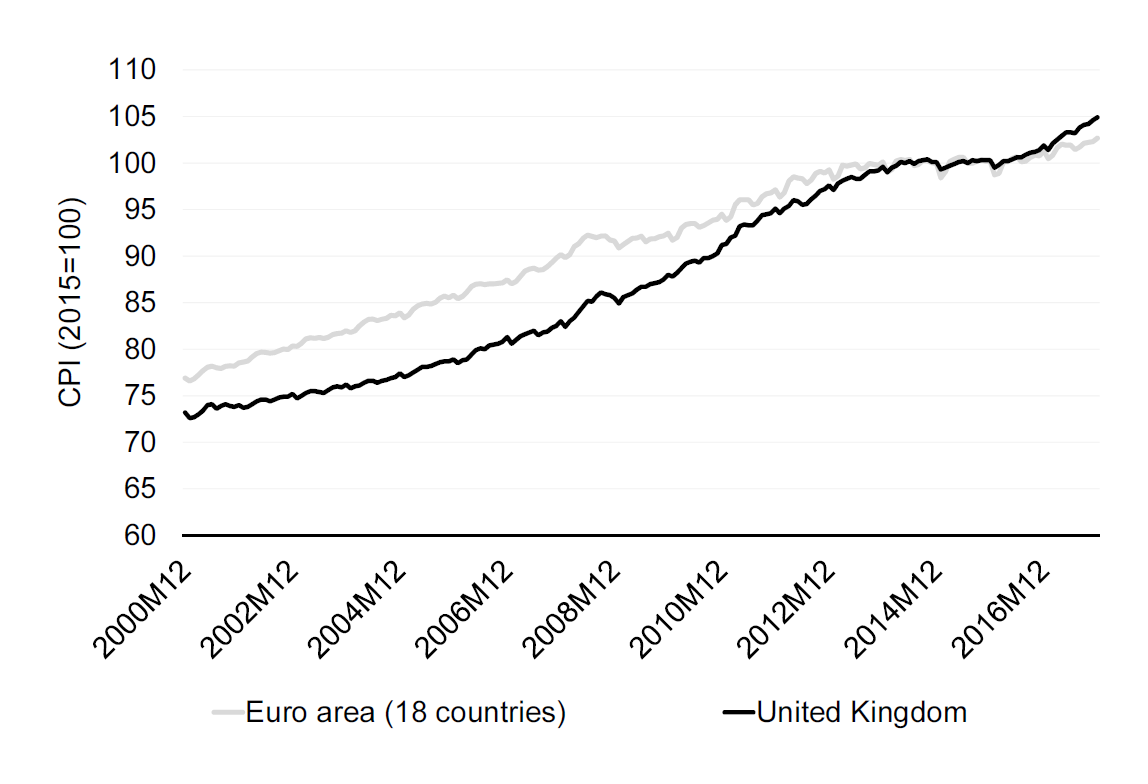
\includegraphics[width=0.75\linewidth]{_resources/chapter_prices/ex1_1} 

}

\caption{The Consumer Price Index (HICP) for the EURO countries and the UK. Source: Eurostat. Notes: The index is constructed such that the 2015 average is 100.}\label{fig:pricefig1}
\end{figure}

\hypertarget{producer-price-index-import-price-index-and-export-price-index}{%
\subsection{Producer Price Index, Import Price Index and Export Price Index}\label{producer-price-index-import-price-index-and-export-price-index}}

Firms typically have different weights than consumers. We typically distinguish between three indexes, the Producer Price Index (PPI), the Import Price Index (IPI) and Export Price Index (EPI). These indexes are all chain-linked Laspeyres-type price index, where weights are updated regularly, but typically less frequent than for consumer price indexes. The weights are constructed using sales data from different sources. For more details see \citep{ppions} for the ONS and \citep{ppieu} for the European level.

\hypertarget{other-indexes-1}{%
\subsection{Other indexes}\label{other-indexes-1}}

A couple of additional indexes also deserve mentioning. First, the GDP deflator. The GDP deflator is considerably broader than the other price indexes, as it covers the complete domestic economy. The National Accounts typically also use chain-linked Laspeyres type approach to be able to make monetary levels comparable across periods. For more details see \citep{gdpons}. Second, the House Price Index (HPI), again a chain-linked Laspeyre type index, with annual updating of weights. This index covers housing bought by households, such as flats, detached houses and terraced houses. Third, the Index of Private Housing Rental Prices (IPHRP) capturing the development in the price tenants face when renting residential housing.

\hypertarget{comparing-monetary-values-across-time}{%
\section{Comparing monetary values across time}\label{comparing-monetary-values-across-time}}

\hypertarget{inflation}{%
\subsection{Inflation}\label{inflation}}

As there are many price indexes, there are also many inflation measures. The Bank of England's inflation target relates to the Consumer Price Index inflation. The ONS publishes both annual and monthly rates, where annual rates relate to the change in prices over a 12 month period, and monthly to a month to month change. As inflation shows the change in price levels, the inflation can be seen as the first derivative of the price index. In Figure \ref{fig:pricefig2} we show the year-to-year change in price levels based on the price indexes shown in Figure \ref{fig:pricefig1}.

\begin{figure}

{\centering 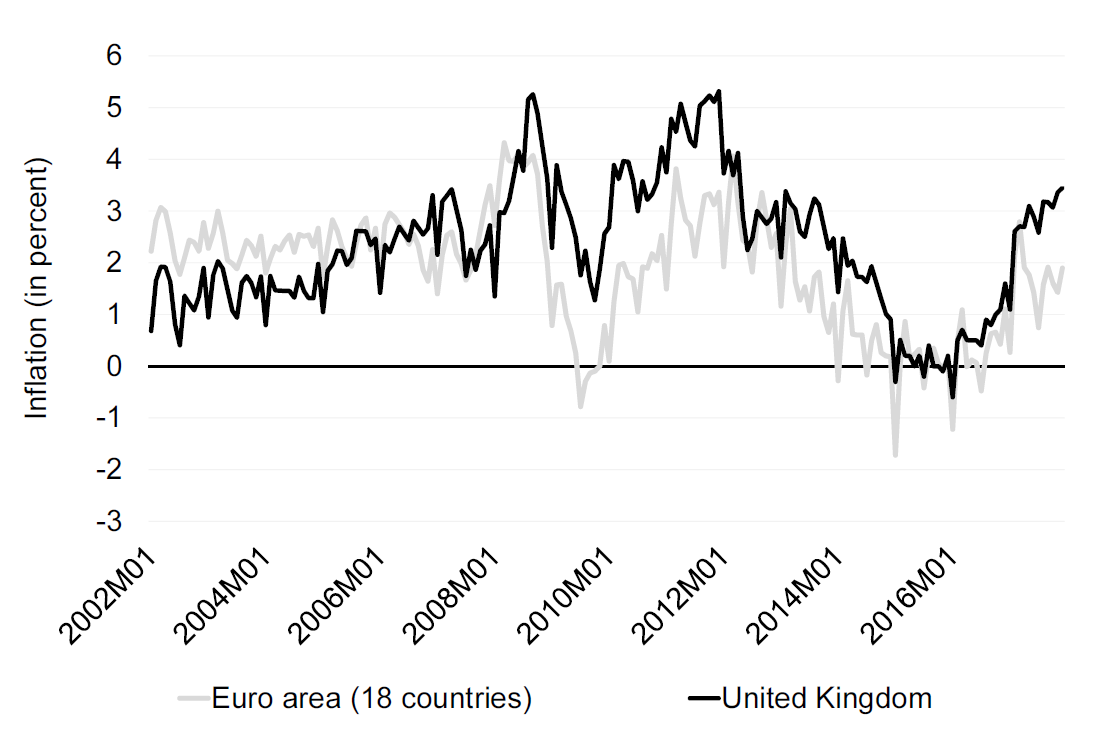
\includegraphics[width=0.75\linewidth]{_resources/chapter_prices/ex1_2} 

}

\caption{Consumer Price Inflation for the EURO countries and the UK. {Source: Eurostat. Notes: The inflation relates to 12 month changes.}}\label{fig:pricefig2}
\end{figure}

Note that the UK inflation is currently considerably higher than the inflation in the EURO area.

\hypertarget{real-vs.-nominal-values}{%
\subsection{Real vs.~nominal values}\label{real-vs.-nominal-values}}

Price indexes are not only used to compute inflation measures. More than 100 years ago, in 1905, the English footballer Alf Common moved from Sunderland to Middlesbrough for a record fee of 1,000 GBP. In terms of today's transfer fees, this sounds unrealistic. But based on the amount you could purchase with 1,000 GBP in 1905, this corresponds to about 114,367 GBP in 2017, which is still low, but seems more reasonable. To make this adjustment, we use price indexes.

Using price indexes we can compare the fee of Alf Common to the fee of for example Kevin Keegan in 1977, when he moved from Liverpool to Hamburg for a fee of 500,000 GBP. The 500,000 GBP in 1977 corresponds to about 2,922,031 GBP in 2017. We can thus refer to the 1,000 GBP and 500,000 GBP as transfer fees in \emph{nominal} terms and the 114,367 GBP and 2,922,031 GBP as \emph{real} terms in the 2017 price level.

\begin{itemize}
\item
  Nominal values are monetary values that are expressed in current prices. For example your monthly income measured in the price level used today or the transfer fee in 1905 measured in the price level of that time.
\item
  Real values are monetary values, where we adjust for changes in price levels. To figure out whether you earn more today than 10 years ago, it is not sufficient just to compare the nominal earnings today and ten years ago, as the price level has changed. As goods and services have become more expensive, the same earnings as 10 years ago, in nominal terms, would enable you to buy less today than ten years ago. Adjusting the earnings to the same price level using inflation or price indexes is necessary to understand whether we are facing a real increase.
\end{itemize}

To convert the nominal values to real values (say the value in the base year) we multiply the nominal values with the change in the price index:

\begin{align}
    P_{BASE}=P_t\times \frac{CPI_{BASE} }{CPI_t}
\end{align}

\hypertarget{the-real-interest-rate}{%
\subsection{The real interest rate}\label{the-real-interest-rate}}

In lecture 13 we discussed interest rates. An annual interest rate of 2 percent means that if I place 100 GBP in that investment, I will receive 102 GBP in one year. But what if the price index also increases from 100 to 102? In real terms I am not richer in a year than I am now, because the same bundle of goods that I am able to buy for 100 GBP today, costs 102 GBP in one year. If we want to know whether we will actually get richer from an investment, we should consider the \emph{real interest rate}. Now let us consider how much richer we are in a year. We want to know the real interest rate \(r\), and we know the nominal interest rate \(i\) and the inflation rate \(\pi\) (it is fairly standard to use these letters for interest rates and inflation). We can thus write

\begin{align}
    1+r= \frac{(1+i)}{(1+\pi)}
\end{align}

which we can rewrite as:

\begin{align}
    1+\pi+r+r\times \pi&= 1+i\nonumber\\
 \Rightarrow    r&= i-\pi-r\times \pi
\end{align}

As inflation and the interest rates typically are fairly small, the term ``\(r\times \pi\)'' will be close to zero. We can therefore compute the approximate real interest rate as:

\begin{align}
    r\approx i-\pi
\end{align}

which is also known as the \emph{Fisher equation}. When inflation exceeds the real interest rate, we face a negative real interest rate.

\hypertarget{the-phillips-curve}{%
\subsection{The Phillips Curve}\label{the-phillips-curve}}

The Phillips curve was introduced by William Phillips an economist from New Zealand. He studied the relationship between inflation and unemployment, a relationship that is visualized in the Phillips Curve. The original Phillips is a scatter plot of wage inflation and unemployment in the UK. The curve showed that periods with low unemployment rates also tended to be periods with high inflation rates, and periods with high unemployment rates also tend to be periods with low inflation. The (short-run) intuition behind this relationship is that when employment is high, the pressure on wages is high, and wage inflation is high. For details on the Phillips curve, see \citep[p.~646 in][]{core} .

In 2008 Gregor \citep{smith2008japan} published a paper, where he showed how the Phillips of Japan looks like Japan. His plot is shown in Figure \ref{fig:pricejapan}, along with a picture from Google maps, of Japan. What do you think? Is this advanced chartjunk?

\begin{figure}

{\centering 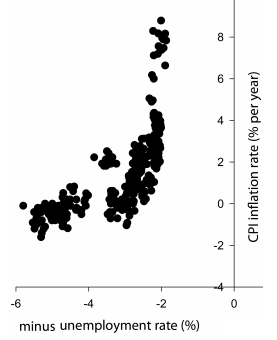
\includegraphics[width=0.5\linewidth]{_resources/chapter_prices/japan4} \includegraphics[width=0.5\linewidth]{_resources/chapter_prices/japan3} 

}

\caption{The Phillips curve of Japan and a map of Japan. Source: The Map is from Google Maps, the Phillips curve is from citet{smith2008japan}. The unemployment rate is multiplied by minus 1. }\label{fig:pricejapan}
\end{figure}

\hypertarget{comparing-monetary-values-across-regions}{%
\section{Comparing monetary values across regions}\label{comparing-monetary-values-across-regions}}

\hypertarget{the-big-mac-index}{%
\subsection{The Big Mac index}\label{the-big-mac-index}}

Considering price levels is not only important when we compare changes over time, but also across countries. In lecture 3 we discussed exchange rates, but sometimes it is not sufficient to just apply the exchange rate. Imagine that you would like to compare the earnings of a typical worker in Ukraine to the earnings of a typical worker in Switzerland. But prices in Ukraine are very different to prices in Switzerland, and just comparing the earnings using the exchange rates would not reflect the differences in living standards. One illustration of the difference is the Big Mac Index, which has been published by the Economist since 1986. According to the 2017 version of the index, a Big Mac costs around 6.35 USD in Switzerland and 1.54 USD in Ukraine. The price level, as approximated with the Big Mac Index is therefore about four times higher in Switzerland compared to Ukraine. If the Big Mac price level is reflective of the overall costs, it would suggest that to obtain the same living standards in Switzerland as in Ukraine, you need about four times the income Switzerland compared to Ukraine.

Several indexes have been produced to mimic the idea of the Big Mac Index (the IPod index, the Starbucks Latte index, etc.). However, these indexes have some obvious short-comings. The product is not the same across countries and the product is not representative of the overall costs.

\hypertarget{purchasing-power-parity}{%
\subsection{Purchasing Power Parity}\label{purchasing-power-parity}}

While the Big Mac Index provides a very simple approach to compare prices. A more rigorous way to compare nominal values across countries is by means of purchasing power parity (PPP). As a point of departure, let us consider the price of a Big Mac. In Switzerland the price is approximately 6.50 CHF and in the US the price is approximately 5.06 USD. This would suggest an exchange rate between US and Switzerland of:

\begin{align}
    PPP_{BigMac,SUIUS}=\frac{6.50}{5.06}=1.28
\end{align}

now, according to the law of one price, we would expect the price of a big mac to be the same in the US and in Switzerland, so the difference must be the exchange rate. Having 5.06 USD must thus be the same as having 6.5 Swiss Francs, or having 1 USD must correspond to 1.28 Swiss Franc. However, at the time of the Big Mac price difference (January 2017), the USD to the CHF exchange rate was 1.01. According to the Big Mac index, the Swiss Franc was overvalued by about 30 percent compared to the USD. So to make the monetary values comparable across Switzerland and the US we multiply all US values with 1.28 instead of the actual exchange rate. We say that the purchasing power parity is 1.28 CHF to 1 USD.

Just like a basket of goods is used to compare prices across time, a representative basket of goods is used to compare prices across countries. The OECD and Eurostat cooperate in the measuring of the PPP. Details on how to compute the PPP can be found in \citep{ppp}. We use PPP to compare GDP (and especially GDP per capita) across countries. Which we will work on in lecture 15

\hypertarget{summary-3}{%
\section{Summary}\label{summary-3}}

In this lecture we've covered the following topics:

\begin{itemize}
\tightlist
\item
  The objective of price indexes.
\item
  Indexes in theory: The Paasche and Laspeyre price indexes.
\item
  Indexes in practice: The Consumer Price index and friends.
\item
  The use of price indexes: computing inflation rates and converting nominal values to real values.
\item
  The Phillips curve.
\item
  Comparing prices across countries using the Purchasing Power Parity.
\end{itemize}

\hypertarget{money}{%
\chapter{Money}\label{money}}

\hypertarget{about-this-chapter-4}{%
\section{About this chapter}\label{about-this-chapter-4}}

If you ask a bank to lend you money, they will probably charge you an interest rate. The interest rate is the price of money. This chapter is about the different types of interest rates, and the price of money in other currencies, the exchange rates.

\hypertarget{intended-learning-outcomes-4}{%
\subsection{Intended learning outcomes}\label{intended-learning-outcomes-4}}

After reading this chapter

\begin{itemize}
\tightlist
\item
  Distinguish between the policy interest rate, the interbank rate, and the bank lending rate.
\item
  To express the price of currencies in terms of exchange rates and describe movements in exchange rates.
\end{itemize}

\hypertarget{interest-rates}{%
\section{Interest rates}\label{interest-rates}}

\hypertarget{the-basics-what-is-the-interest-rate}{%
\subsection{The basics: What is the interest rate?}\label{the-basics-what-is-the-interest-rate}}

If you ask a friend whether you can borrow 2 GBP today, it is likely, that you have repaid your debt once you've repaid these 2 GBP. However, if you ask your bank whether you can borrow 10,000 GBP, it is likely that they will require you to repay more than 10,000 GBP. If the bank asks you to repay 10,500 GBP, the bank charged you an interest of 5 percent rate. Or in other words, the interest rate, \(i\), on your bank loan is 5 percent:

\begin{align}
    i=\frac{\text{amount to repay}}{\text{amount borrowed}}-1=\frac{10,500}{10,000}-1=0.05
\end{align}

Why did you have to pay more to the bank than you borrowed? To be able to lend 10,000 GBP to you, the bank has to get 10,000 GBP from somewhere. Banks borrow and lend money on the \emph{money market} where they also pay an interest rate for lending money. Alternatively the bank could lend the money from another customer, but this other customer would expect to get something in return, an interest.

Why would the other costumer expect an interest? The short answer: Money \emph{today} is costly. Would I rather have 100 GBP today or 100 GBP in two years? If you take 100 GBP today you could just keep the money in a safe place for two years. So money today should be at least as much worth today as in two years (everything else equal). Moreover over two years things might get more expensive. The amount of goods you can buy today for 100 GBP is probably larger than the amount of goods you can buy in two years because of the inflation. Moreover, you could also keep the 100 GBP today and invest them in stocks or bonds, and you might have more than 100 GBP in two years. So in sum, money today is typically more worth than money at a later point in time, and you have to pay a price for for that, the interest rate.

Why are interest rates important in economics? Imagine that you have a business idea, and that you need some funding, say 10,000 GBP. You go to your bank and ask for 10,000 GBP today. They might answer, sure just promise to give us 10,050 GBP in ten years. That is an interest rate of 0.5 percent (\(=100*((10,500/10,000)-1)\)). Not a bad deal, and you might be inclined to accept it and start your own business. But imagine that the bank says, sure, just promise to give us 20,000 GBP in ten years. That is an interest rate of 100 percent (\(=100*((20,000/10,000)-1)\)). Unless you have no other (cheaper) options to borrow money and you are very certain of your business idea, you will be probably reject this offer and not initiate your business idea. So the interest rate can affect the activity in the economy. A low interest rate means that it is cheap to borrow money. You can borrow money to start a new business, to buy a new car or to renovate your house. Buying new cars affects the auto mobile industry and renovating the house might affect jobs for carpenters and bricklayers.

But a low interest rate might also discourage savings, because when interest rates are low, the return on saving money is low. If banks are offering loans for 0.5 percent they probably paid less than 0.5 percent to borrow the money themselves, so saving money is also less attractive. But what determines the interest rates? \citep[chapter 10 in][]{core} provides a nice introduction to the money and credit market. We will provide a brief and very simplified description of the different interest rates in the next section.

\hypertarget{three-interest-rates}{%
\subsection{Three interest rates}\label{three-interest-rates}}

Let us consider an extremely simplified version of the money market:

\begin{itemize}
\tightlist
\item
  The central bank controls the money supply and sets the interest rate. The interest rate set by the central bank is called the \emph{policy interest rate} or the base rate. Commercial banks can borrow money at these rates.
\item
  Commercial banks can also borrow and lend money to each other on the interbank lending market at the \emph{interbank rate}.
\item
  Commercial banks lend money to households and firms at the \emph{bank lending rate}.
\end{itemize}

So what happens when you ask your bank for a loan?

\begin{itemize}
\tightlist
\item
  If your bank has sufficient funds it will just provide you a loan at their bank lending rate.
\item
  If the bank does not have sufficient funds it will try to borrow money on the money market, either from the central bank or from other banks.
\end{itemize}

You will most likely pay a higher interest rate than the bank is paying the central bank or other banks. Even though the interest rate you pay for a bank loan is not the same as the interest rate your bank pays on the interbank market, there is a relationship between these rates. When central banks lower the policy interest rates, it becomes cheaper for banks to borrow money and they can offer you a loan at a lower price. Given that there is competition in the commercial bank market, it is likely that they will lower the interest they charge you, if their costs are reduced. Figure \ref{fig:money1} shows a line chart of the policy interest rate and the commercial bank lending rate for the UK.

\begin{figure}

{\centering 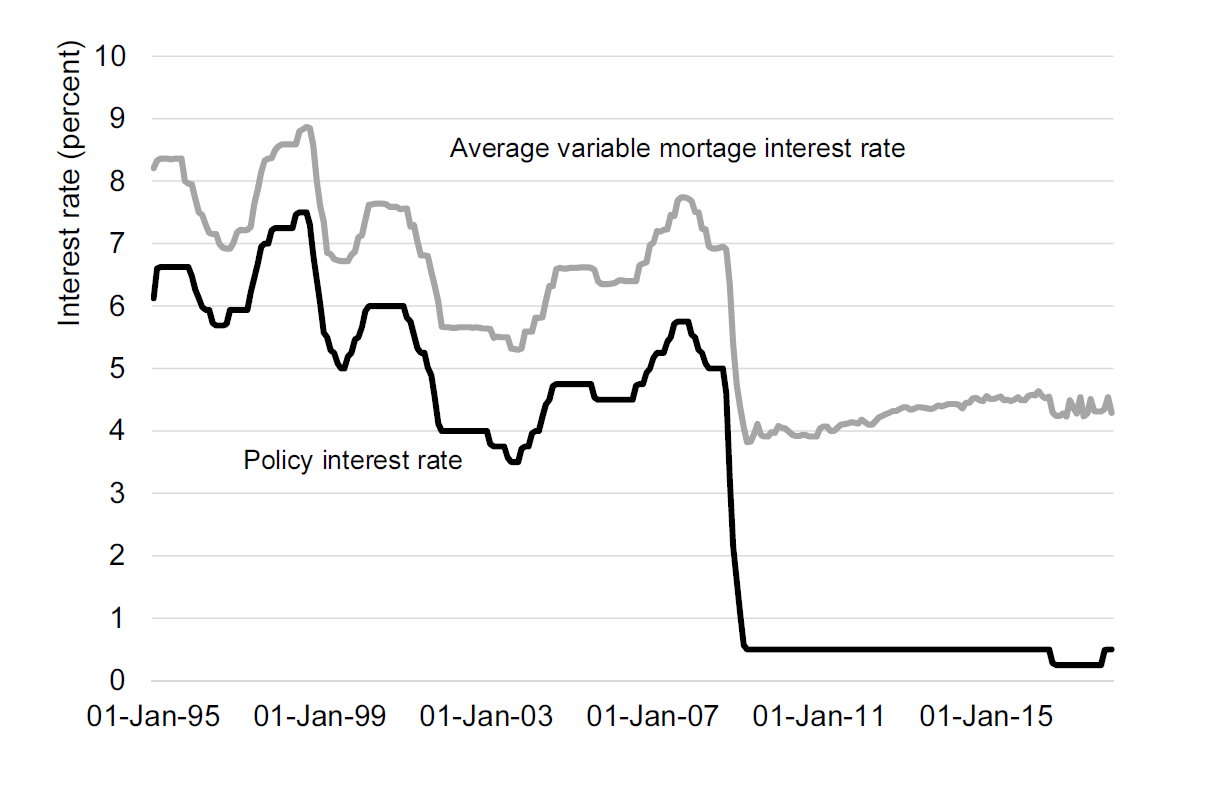
\includegraphics[width=0.7\linewidth]{_resources/chapter_money/ex4_2} 

}

\caption{Policy interest rates and bank interest rates for the UK. Source: Bank of England. Series: IUMABEDR and IUMTLMV.}\label{fig:money1}
\end{figure}

You clearly see in Figure \ref{fig:money1} that the policy interest rate by the Bank of England and the average interest rate charged by commercial banks (the bank lending rage) follow each other. When the price of money falls, ie. the policy interest rate falls, the price banks charge on mortgages also falls. However, note that after the financial crisis, the gap between these two interest rates has increased. Figure \ref{fig:money2} shows the gap (in percentage points) over the same time period. After the financial crisis the gap increased form approximately two percentage points to four percentage points. Why do you think this is the case?

\begin{figure}

{\centering 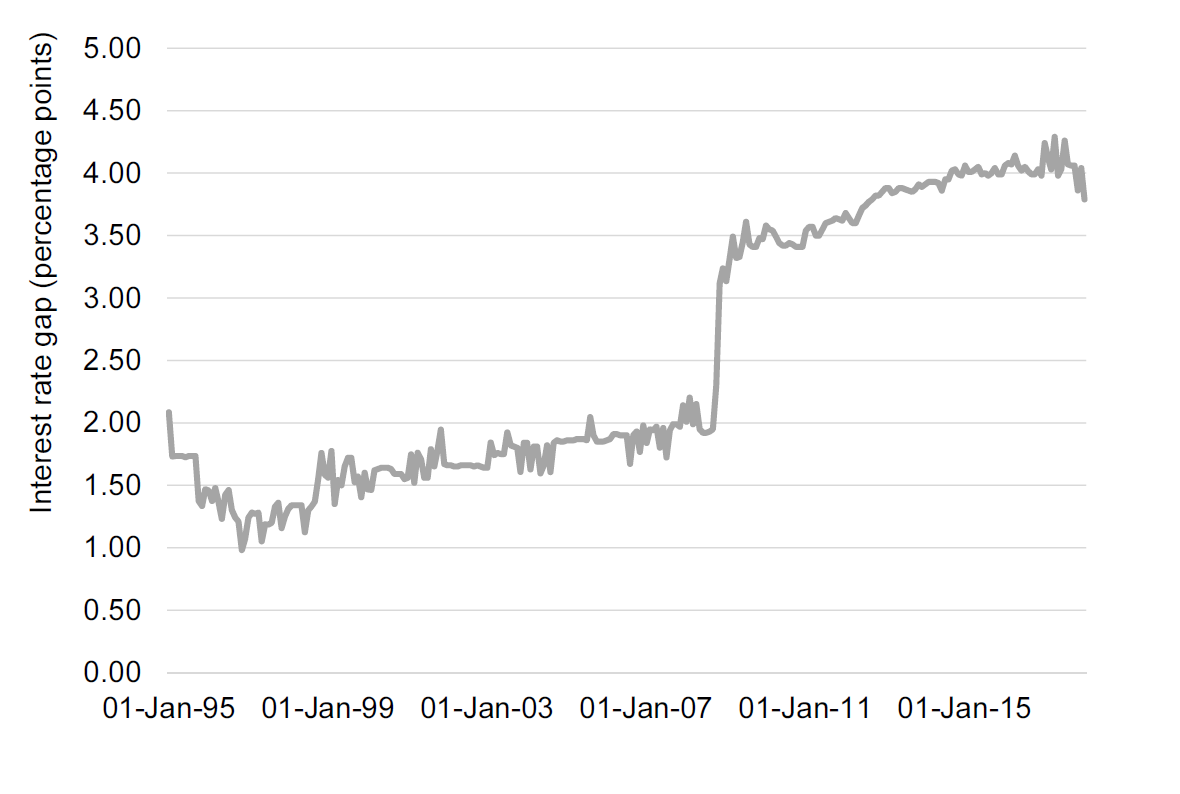
\includegraphics[width=0.7\linewidth]{_resources/chapter_money/ex4_3} 

}

\caption{The Gap between the policy interest rate and bank interest rate for the UK. Source: Bank of England. Series: IUMABEDR and IUMTLMV.}\label{fig:money2}
\end{figure}

However, there is not only one commercial bank lending rate, there are many. The interest rate the bank charges you, not only depends on their direct costs, but also on the risk they are facing. Mortgages are secured in the property, such that if the loan is not repaid, the money lender can use the property as a compensation, for example by selling the property. This means that mortgages have a relatively high degree of security for the lender. However, some loans have almost no security, for example overdraft loans or credit card loans.
Figure \ref{fig:money3} shows the average overdraft interest rate for the same period. There is no clear relationship between the interest rate on overdrafts and the interest rate and the policy interest rate. Why do you think this is the case?

\begin{figure}

{\centering 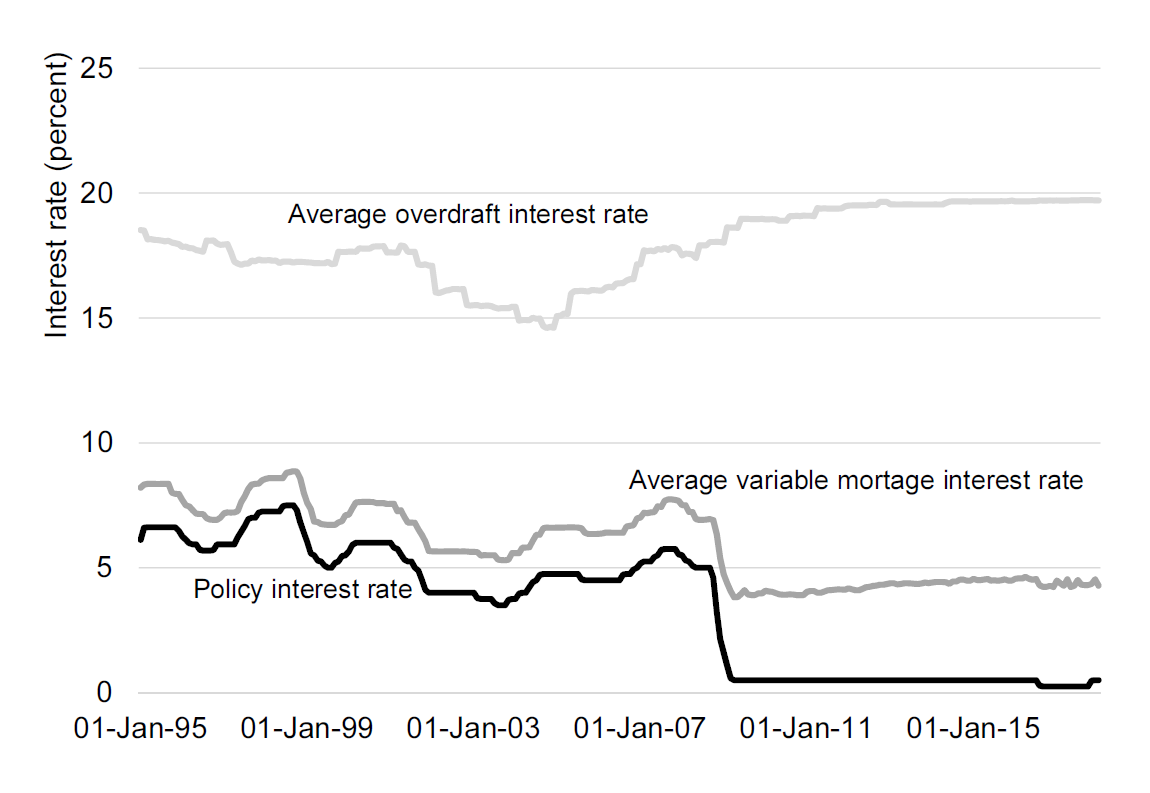
\includegraphics[width=0.7\linewidth]{_resources/chapter_money/ex4_1} 

}

\caption{The policy interest rate, the  bank interest rate (mortgages) for the UK and the overdraft interest rates. Source: Bank of England. Series: IUMABEDR, IUMODTL and IUMTLMV..}\label{fig:money3}
\end{figure}

In addition to risk, the timespan of the repayment also affects the interest rate. If you would like to repay your loan over a longer period, the bank is likely to charge a higher price. Some bank loans have a fixed interest rate and some have a flexible interest rate. With a fixed interest rate, you know exactly what price you are paying throughout the repayment period. With a flexible interest rate, the costs of the loan might change. Finally it is important to consider how frequent the interest rate is accumulated. On many overdraft loans, the interest is calculated on a daily basis. Interest rates usually refer to annual rates.

\hypertarget{getting-data-on-interest-rates}{%
\subsection{Getting data on interest rates}\label{getting-data-on-interest-rates}}

TBD

\hypertarget{summary-interest-rates}{%
\subsection{Summary: Interest rates}\label{summary-interest-rates}}

\emph{Definition}
* The price of money.
* The relative difference between what you pay compared to what you borrowed.

\emph{Interest rates}
* The Policy interest rate: Set by the central bank, also known as the base rate, or for the UK: BOEBR (Bank of England base rate).
* Interbank interest rate: The rate banks charge each others for loans. In the UK: LIBOR (London Inter-bank Offered Rate)
* Commercial bank lending rates.

\emph{Factors affecting the interest rate}

\begin{itemize}
\tightlist
\item
  The cost of obtaining money (i.e.~the base rate and the interbank interest rate).
\item
  The risk of the loan.
\item
  The time span of the loan.
\item
  Whether the interest rate is fixed or flexible.
\end{itemize}

\hypertarget{exchange-rates}{%
\section{Exchange rates}\label{exchange-rates}}

\hypertarget{definition-of-exchange-rates}{%
\subsection{Definition of exchange rates}\label{definition-of-exchange-rates}}

Exchange rates describe the value of one currency relative to another currency. Specifically it says how many units of one currency we can buy from one unit of another currency. This causes a lot of confusion, because the ordering of the units get mixed up. Importantly the currency that comes after the ``to the'' is always the currency that you consider one unit of. One way to remember this is to always add an ``buy one unit of'' between the ``to'' and the ``the'':

\begin{center}
    "An exchange rate of \emph{Y} \emph{currency a} to (buy one unit of) the \emph{currency b}."
\end{center}

An example:

\begin{center}
    An exchange rate of 1.39 US Dollar to  the British Pound.\vspace{12pt}\\
    means:\vspace{12pt}\\
    An exchange rate of 1.39 US Dollar to \emph{buy one unit of} the British Pound.\\
\end{center}

As with interest rates, there are several exchange rates. The exchange rate is determined on the foreign exchange market (FOREX). It is mostly large banks and financial institutions that buy and sell on FOREX. When we individuals buy or sell foreign currencies, we typically just go to our local bank or to business that specialize in exchanging currencies. We rarely pay the same exchange rate as on the FOREX, because we also pay some sort of commission to the local bank or currency exchanger.

\hypertarget{ups-and-downs-appreciation-and-depreciation}{%
\subsection{Ups and downs: appreciation and depreciation}\label{ups-and-downs-appreciation-and-depreciation}}

When exchange rates go up or down we use the terms appreciation and depreciation. When a currency depreciates it loses value compared to the foreign currency. When a currency appreciates it gains value. Figure \ref{fig:money4} shows the price of one USD in EURO increased substantially in the beginning of 2015. In other words 1 EURO became less worth compared to the USD, so it depreciated. Vice versa in 2017, where the price of a USD in EURO went down, so that the EURO depreciated.

\begin{figure}

{\centering 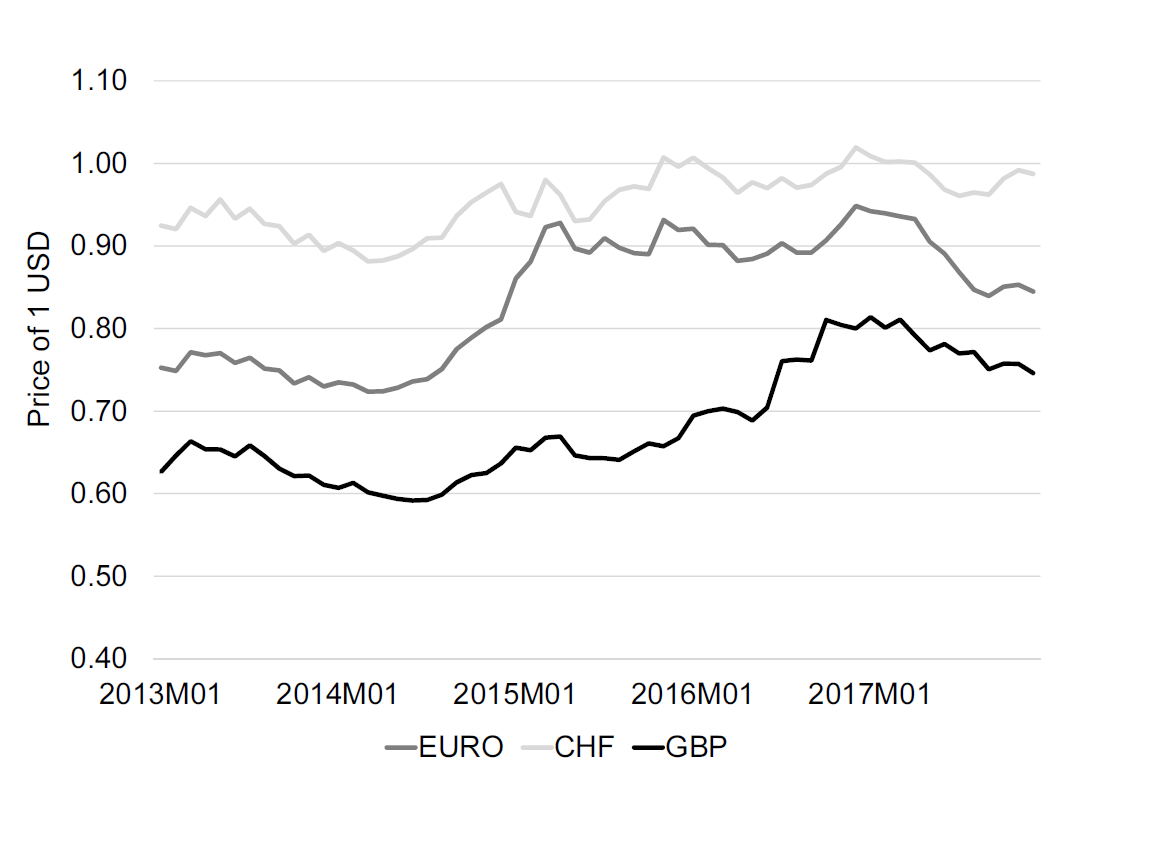
\includegraphics[width=0.7\linewidth]{_resources/chapter_money/ex5} 

}

\caption{Exchange rates: EURO, CHF, GBP to USD. Source: The IMF.}\label{fig:money4}
\end{figure}

\hypertarget{summary-exchange-rates}{%
\subsection{Summary: Exchange rates}\label{summary-exchange-rates}}

\emph{Definition}
* The value of one currency relative to another currency: \textbf{An exchange rate of Y currency a to (buy one unit of) the currency b}

\emph{Ups and downs}

\begin{itemize}
\tightlist
\item
  Appreciation: A currency's value increases relative to the foreign currency.
\item
  Depreciation: A currency's value decreases relative to the foreign currency.
\end{itemize}

\emph{Interbank and commercial exchange rates}
* Commercial exchange rates: The exchange rate you pay in the bank or the supermarket.
* Interbank exchange rate: The exchange rate your bank pay on the interbank market.

\hypertarget{getting-data-on-exchange-rates}{%
\subsection{Getting data on exchange rates}\label{getting-data-on-exchange-rates}}

TBD

\hypertarget{linking-interest-rates-and-exchange-rates}{%
\section{Linking interest rates and exchange rates}\label{linking-interest-rates-and-exchange-rates}}

So we've talked about interest rates and exchange rates. Is there a link between these rates? We know that the interest rates are affected by national banks, that set national policy interest rates. But what determines the exchange rates? If a currency is free-floating, the exchange rate is determined on the market by supply and demand. If more people want to hold GBP, the price will increase.

Who invests in currencies? Mostly international investors. And these investors like high returns, so they want to hold assets that pay high returns. When the policy interest rate is lowered, the interest rate on the country's financial assets such as bonds goes down, making them less attractive. This will lower the demand for for assets. And thus also for the currency, and ultimately, the asset will depreciate.

You can read much more about the link between exchange rates and interest rates in \citep[chapter 15 in][]{core}.

\hypertarget{summary-4}{%
\section{Summary}\label{summary-4}}

In this chapter we have covered the following topics:

\begin{itemize}
\item
  The three types of interest rates:

  \begin{itemize}
  \tightlist
  \item
    The policy interest rate: the interest rate set by central banks and charges banks.
  \item
    The interbank rate: the interest rate banks charge each other.
  \item
    The bank lending rate: the interest rates banks charge normal household.
  \end{itemize}
\item
  Expressing the price of foreign currencies in terms of exchange rates.
\item
  Currency appreciation and depreciation.
\item
  The link between interest rates and exchange rates.
\end{itemize}

\hypertarget{the-labor-market}{%
\chapter{The labor market}\label{the-labor-market}}

\hypertarget{about-this-chapter-5}{%
\section{About this chapter}\label{about-this-chapter-5}}

This chapter is about the labor market. We start with a description of how we can divide the population into groups according to economic activity. We discuss how we define employment and unemployment and two ways of measuring unemployment rates. We will also discuss the difference between the intensive and extensive margin of labor supply and briefly describe how we can quantify the demand side of the labor market and create a graphical representation of the matching efficiency in the labor market by means of the Beveridge curve.

\hypertarget{indend-learning-outcomes}{%
\subsection{Indend learning outcomes}\label{indend-learning-outcomes}}

After reading this chapter you should be able to

\begin{itemize}
\tightlist
\item
  Explain and apply definitions of unemployment rates:

  \begin{itemize}
  \tightlist
  \item
    The survey based measure of unemployment.
  \item
    The register based measure of unemployment.
  \end{itemize}
\item
  Explain the difference between the extensive and intensive margin of labor supply.
\item
  Create data visualizations of labor demand and the Beveridge curve.
\end{itemize}

\hypertarget{from-population-data-to-the-labor-market}{%
\section{From population data to the labor market}\label{from-population-data-to-the-labor-market}}

\hypertarget{grouping-the-population-according-to-economic-activity}{%
\subsection{Grouping the population according to economic activity:}\label{grouping-the-population-according-to-economic-activity}}

We have now described levels and movements in the population numbers. We will now divide the population in groups according to their \emph{economic activity}. For economic analyses it is often useful to split the population in four groups: (1) children, (2) elderly, (3) in the labor force and (4) out of the labor force. This distinction is used in most countries, but the exact definitions of groups vary from country to country. One reason for the variation in group definitions is that they are linked to the institutional setting. The definition of what ages are defined as ``children'' will typically depend on the formal compulsory minimum school leaving age. The definition of what ages to include as the elderly will typically depend on the retirement policies. The box below summarizes this and presents the classification used by the Office for National Statistics in the United Kingdom.

\begin{myblock}
\textbf{From the population to labor force}

The full population can be divided into

\begin{itemize}
\item
  Children (ONS definition: Aged below 16)
\item
  Elderly (ONS definition: Aged above 64)
\item
  In the labor force
\item
  Out of the labor force

  The labor force consists of the following two groups:
\item
  People who are unemployed
\item
  People who are employed (including self-employed)

  Out of the labor force consists of the following:
\item
  Students
\item
  Long-term sick
\item
  Looking after family/staying home
\item
  Retired
\item
  Other
\end{itemize}
\end{myblock}

Using the data from the last section we can investigate the development of the age groups, as shown in Figure \ref{fig:labour1}). The area chart is visually appealing , but it is difficult to identify small trends in variables that are not shown at the lowest level.

\textbackslash begin\{figure\}

\{\centering 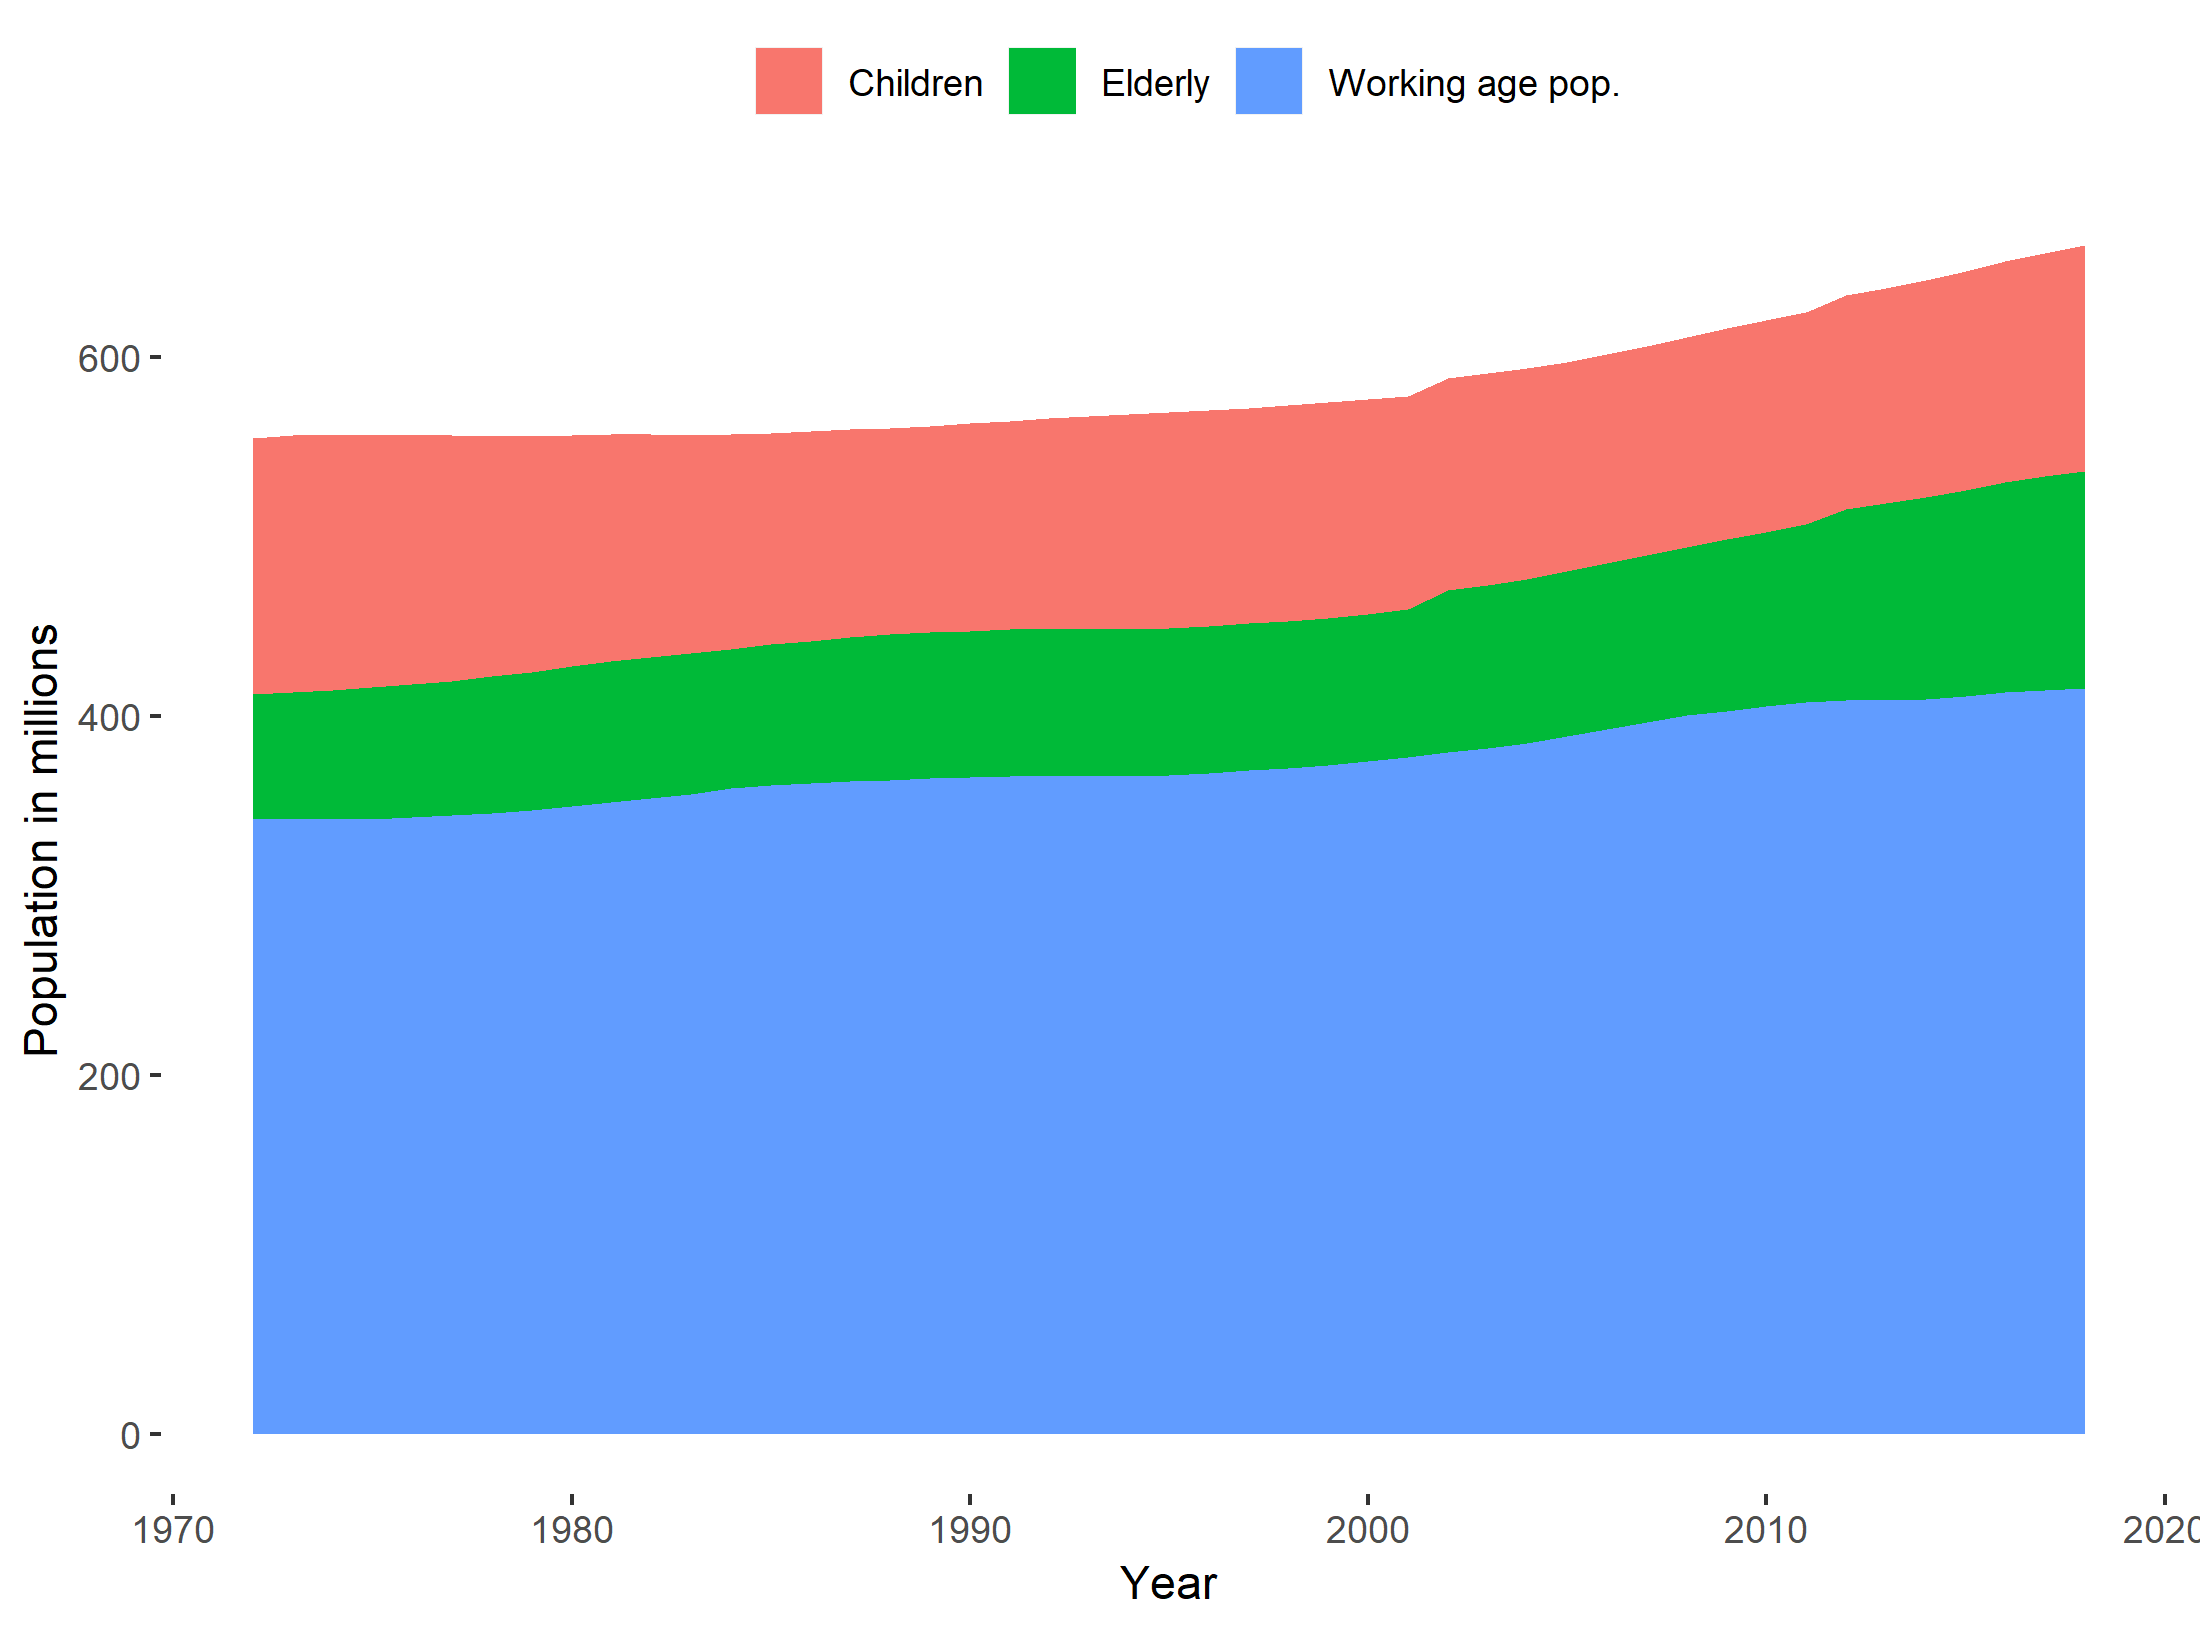
\includegraphics[width=0.7\linewidth]{_resources/chapter_labour/fig13}

\}

\textbackslash caption\{Grouping the population of the United Kingdom by age group. Data source: Eurostat. The R script for this Figure is available \href{https://www.hhsievertsen.net/economicdata/notes/lecture12/rmaterial/lecnote_12_script_for_fig7.R}{here}\}\label{fig:labour1}
\textbackslash end\{figure\}

We will now take a closer a look at the labor force by defining the categories in the labor force.

\hypertarget{unemployment}{%
\section{Unemployment}\label{unemployment}}

\hypertarget{what-is-unemployment}{%
\subsection{What is unemployment?}\label{what-is-unemployment}}

While most people have an idea about what unemployment is, the exact definition of unemployment is considerably less well known. Who is unemployed? Are retired people defined as unemployed? Are children defined as unemployed? Most people would probably say no to these questions. But there are more complex groups: Are students defined as unemployed if they don't work? Are parents on parental leave defined as unemployed? Am I defined as unemployed if I decide not to work? Actually, the answer in all these cases is no (in most cases), according to the international definition of unemployment specified by the International Labour Organisation (ILO). So who is unemployed then? According to the ILO definition, unemployed is being \citep{ons}

\begin{itemize}
\tightlist
\item
  without a job, have been actively seeking work in the past four weeks and are available to start work in the next two weeks
\item
  out of work, have found a job and are waiting to start it in the next two weeks
\end{itemize}

This definition is used by the European Union (Eurostat), by the Organisation for Economic Cooperation and Development (OECD) and many national statistical offices (including the Office for National Statistics in the United Kingdom). But how do we get data on the questions above? The solution is survey data. For the United Kingdom we obtain data on unemployment from the Labour Force Survey (LFS). The LFS is conducted by the Office for National Statistics by selecting random households from the Royal Mail's Postcode Address File.

\hypertarget{an-internationally-coherent-definition-of-unemployment}{%
\subsubsection{An internationally coherent definition of unemployment}\label{an-internationally-coherent-definition-of-unemployment}}

All European Union member states have are obliged to run labor force surveys on at least an annual basis. For the UK, the survey has been quarterly since 1992. The Office for National Statistics also release monthly data, although this is not included in the official statistics.

The ILO unemployment definition above is also called the survey measure of unemployment. This is because the most common alternative measure of unemployment is based on register data from administrative records. Registered unemployment is measured by using data on the number of benefit claimants. Instead of asking people about whether they are looking for a job and not working, we assume that people that claim benefits are unemployed. Statistical offices typically release both measures of unemployment. The register and survey based measures of unemployment typically deviate substantially because:

\begin{itemize}
\tightlist
\item
  People might be looking for jobs even if they don't claim benefits because they are not eligible for benefits.
\item
  People might be claiming benefits without looking for jobs.
\end{itemize}

\begin{myblock}
\textbf{Measuring unemployment: Two definitions}

\emph{1. The survey based measure of unemployment (also known as the ILO
definition).}

\begin{itemize}
\item
  Based on surveys of random subsamples of the population.
\item
  People are defined as unemployed if they are

  \begin{itemize}
  \tightlist
  \item
    without a job, have been actively seeking work in the past four
    weeks and are available to start work in the next two weeks
  \item
    out of work, have found a job and are waiting to start it in the
    next two weeks
  \end{itemize}
\end{itemize}

\emph{2. The register based measure of unemployment.}

\begin{itemize}
\tightlist
\item
  Based on administrative registers of benefit claimants.

  \begin{itemize}
  \tightlist
  \item
    How many individuals received unemployment benefits.
  \end{itemize}
\end{itemize}
\end{myblock}

\hypertarget{employment}{%
\subsection{Employment}\label{employment}}

\hypertarget{an-internationally-coherent-definition-of-employment}{%
\subsubsection{An internationally coherent definition of employment}\label{an-internationally-coherent-definition-of-employment}}

Just like unemployment, measuring employment is not straightforward and the ILO has specified a definition, which the Office for National Statistics applies in the LFS. Following this definition people are employed if they are above 16 and satisfy one of the following conditions:

\begin{itemize}
\tightlist
\item
  work at least one hour for pay in a week, people who are temporarily away from jobs.
\item
  are on Government-supported training/employment programs.
\item
  do unpaid family work.
\end{itemize}

Paid work refers to both employees and self-employed, and unpaid family work refers to working for family business without receiving a formal wage, but still benefiting from the business.

It is important to note that employment is not the same as jobs. Employment measures refers to people, and people with several jobs will only be counted once in the employment statistics. In the job statistics, each job is counted.

Like with unemployment, we can also compute register based measures of employment by using information from income tax payments, insurance status and other administrative registers.

\begin{myblock}
\textbf{Measuring employment: Two definitions}

\emph{1. The survey based measure of employment.}

\begin{itemize}
\tightlist
\item
  work at least one hour for pay in a week, people who are temporarily
  away from jobs.
\item
  are on Government-supported training/employment programs.
\item
  do unpaid family work.
\end{itemize}

\emph{2. The register based measure of employment.}

\begin{itemize}
\tightlist
\item
  information from income tax payments, insurance status and other
  administrative registers.
\end{itemize}
\end{myblock}

\hypertarget{the-unemployment-rate}{%
\subsection{The unemployment rate}\label{the-unemployment-rate}}

\hypertarget{an-internationally-coherent-definition-of-the-labor-force}{%
\subsubsection{An internationally coherent definition of the labor force}\label{an-internationally-coherent-definition-of-the-labor-force}}

Having defined who is unemployed and who is employed it is straightforward to define the labor force. The labor force is simply the sum of these two groups:

\begin{align}
  \text{Labor force}=Unemployed+Employed
\end{align}

\hypertarget{an-internationally-coherent-definition-of-the-unemployment-rate}{%
\subsubsection{An internationally coherent definition of the unemployment rate:}\label{an-internationally-coherent-definition-of-the-unemployment-rate}}

We are now ready to calculate the unemployment rate. The unemployment rate is the fraction of the labor force that is unemployed:

\begin{align}
  \text{Unemployment rate}&=\frac{Unemployed}{\text{Labor force}}\nonumber\\
  &=\frac{Unemployed}{Unemployed+Employed}
\end{align}

How can the unemployment rate change? If people move from unemployment to employment, the unemployment rate clearly goes down, as the size of the denominator is unchanged and the size of the numerator is reduced. Vice versa if people move from employment to unemployment.

What happens to the unemployment rate if people move from unemployment to out of the labor force? The unemployment rate will go down, everything else equal, because the numerator is increased by relatively more than the numerator. Vice versa if people go from out of the labor force to unemployment.

\hypertarget{the-unemployment-rate.-an-illustration-using-data-for-united-kingdom}{%
\subsubsection{The unemployment rate. An illustration using data for United Kingdom}\label{the-unemployment-rate.-an-illustration-using-data-for-united-kingdom}}

Figure \ref{fig:labour2} shows the unemployment rate for the United Kingdom using both measures. As you can see, for the period considered, the registered unemployment rate is always lower than the survey based measure of unemployment. Why do you think this is the case? And why is the difference not constant over time?

\textbackslash begin\{figure\}

\{\centering 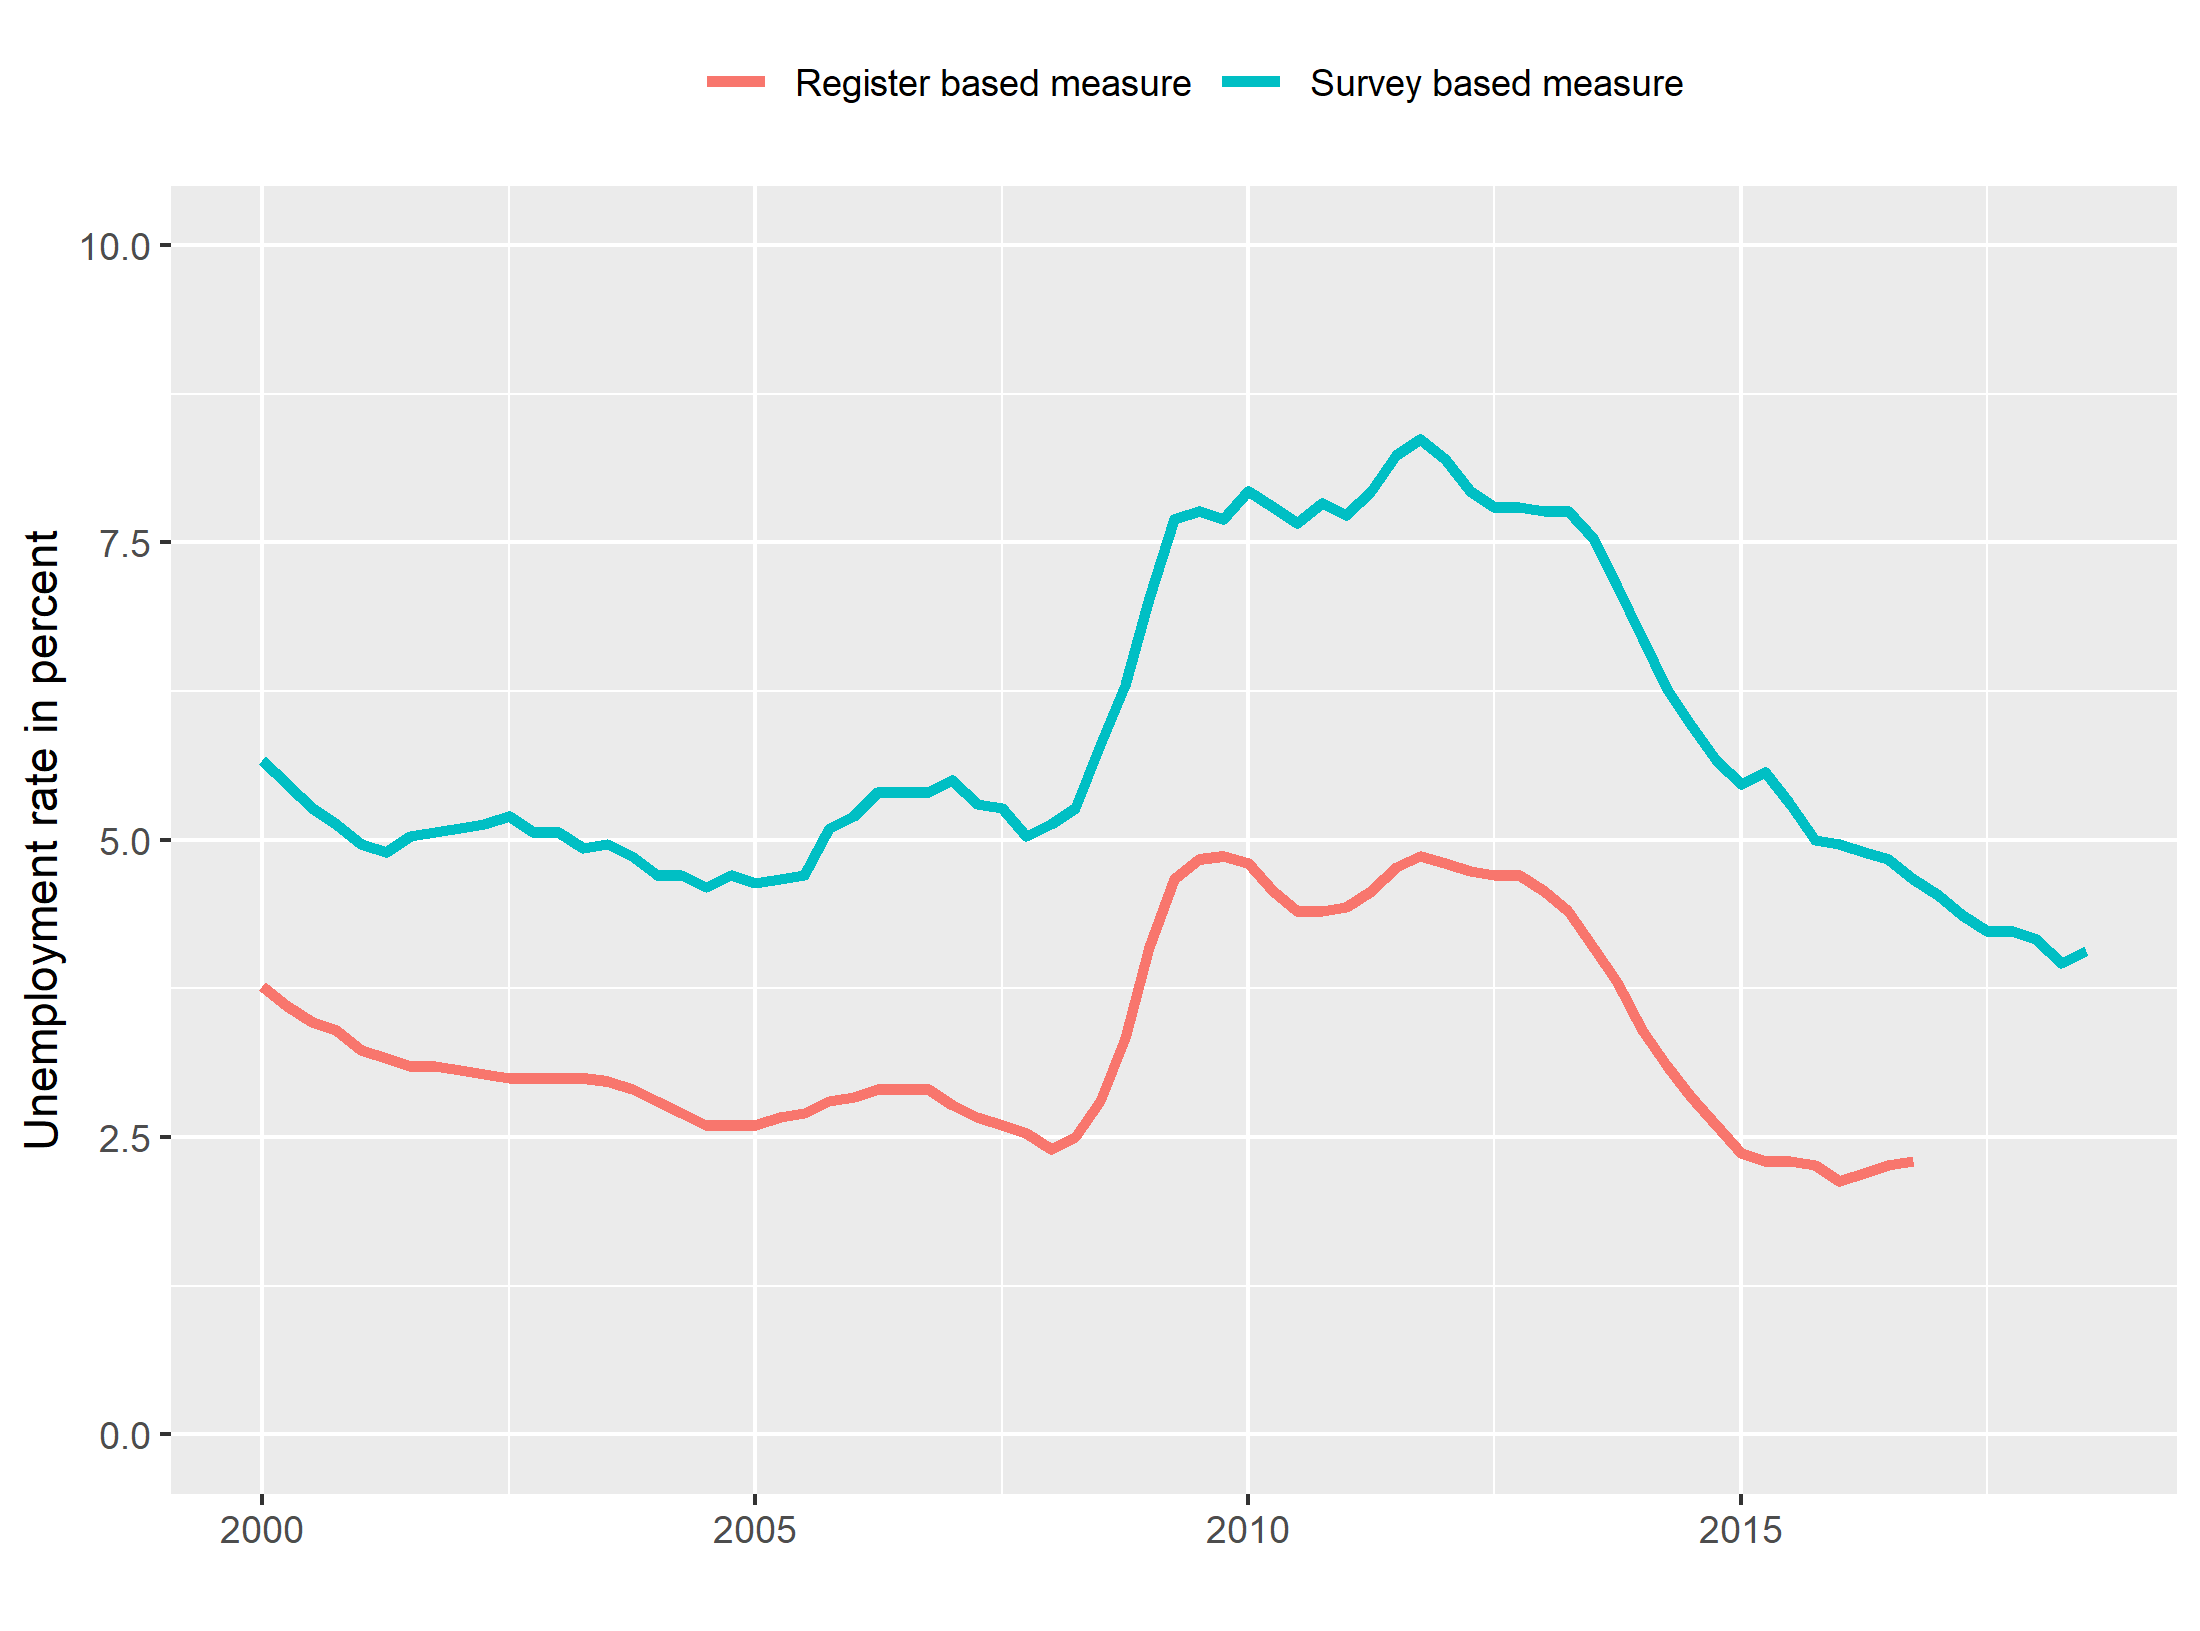
\includegraphics[width=0.49\linewidth]{_resources/chapter_labour/fig14} 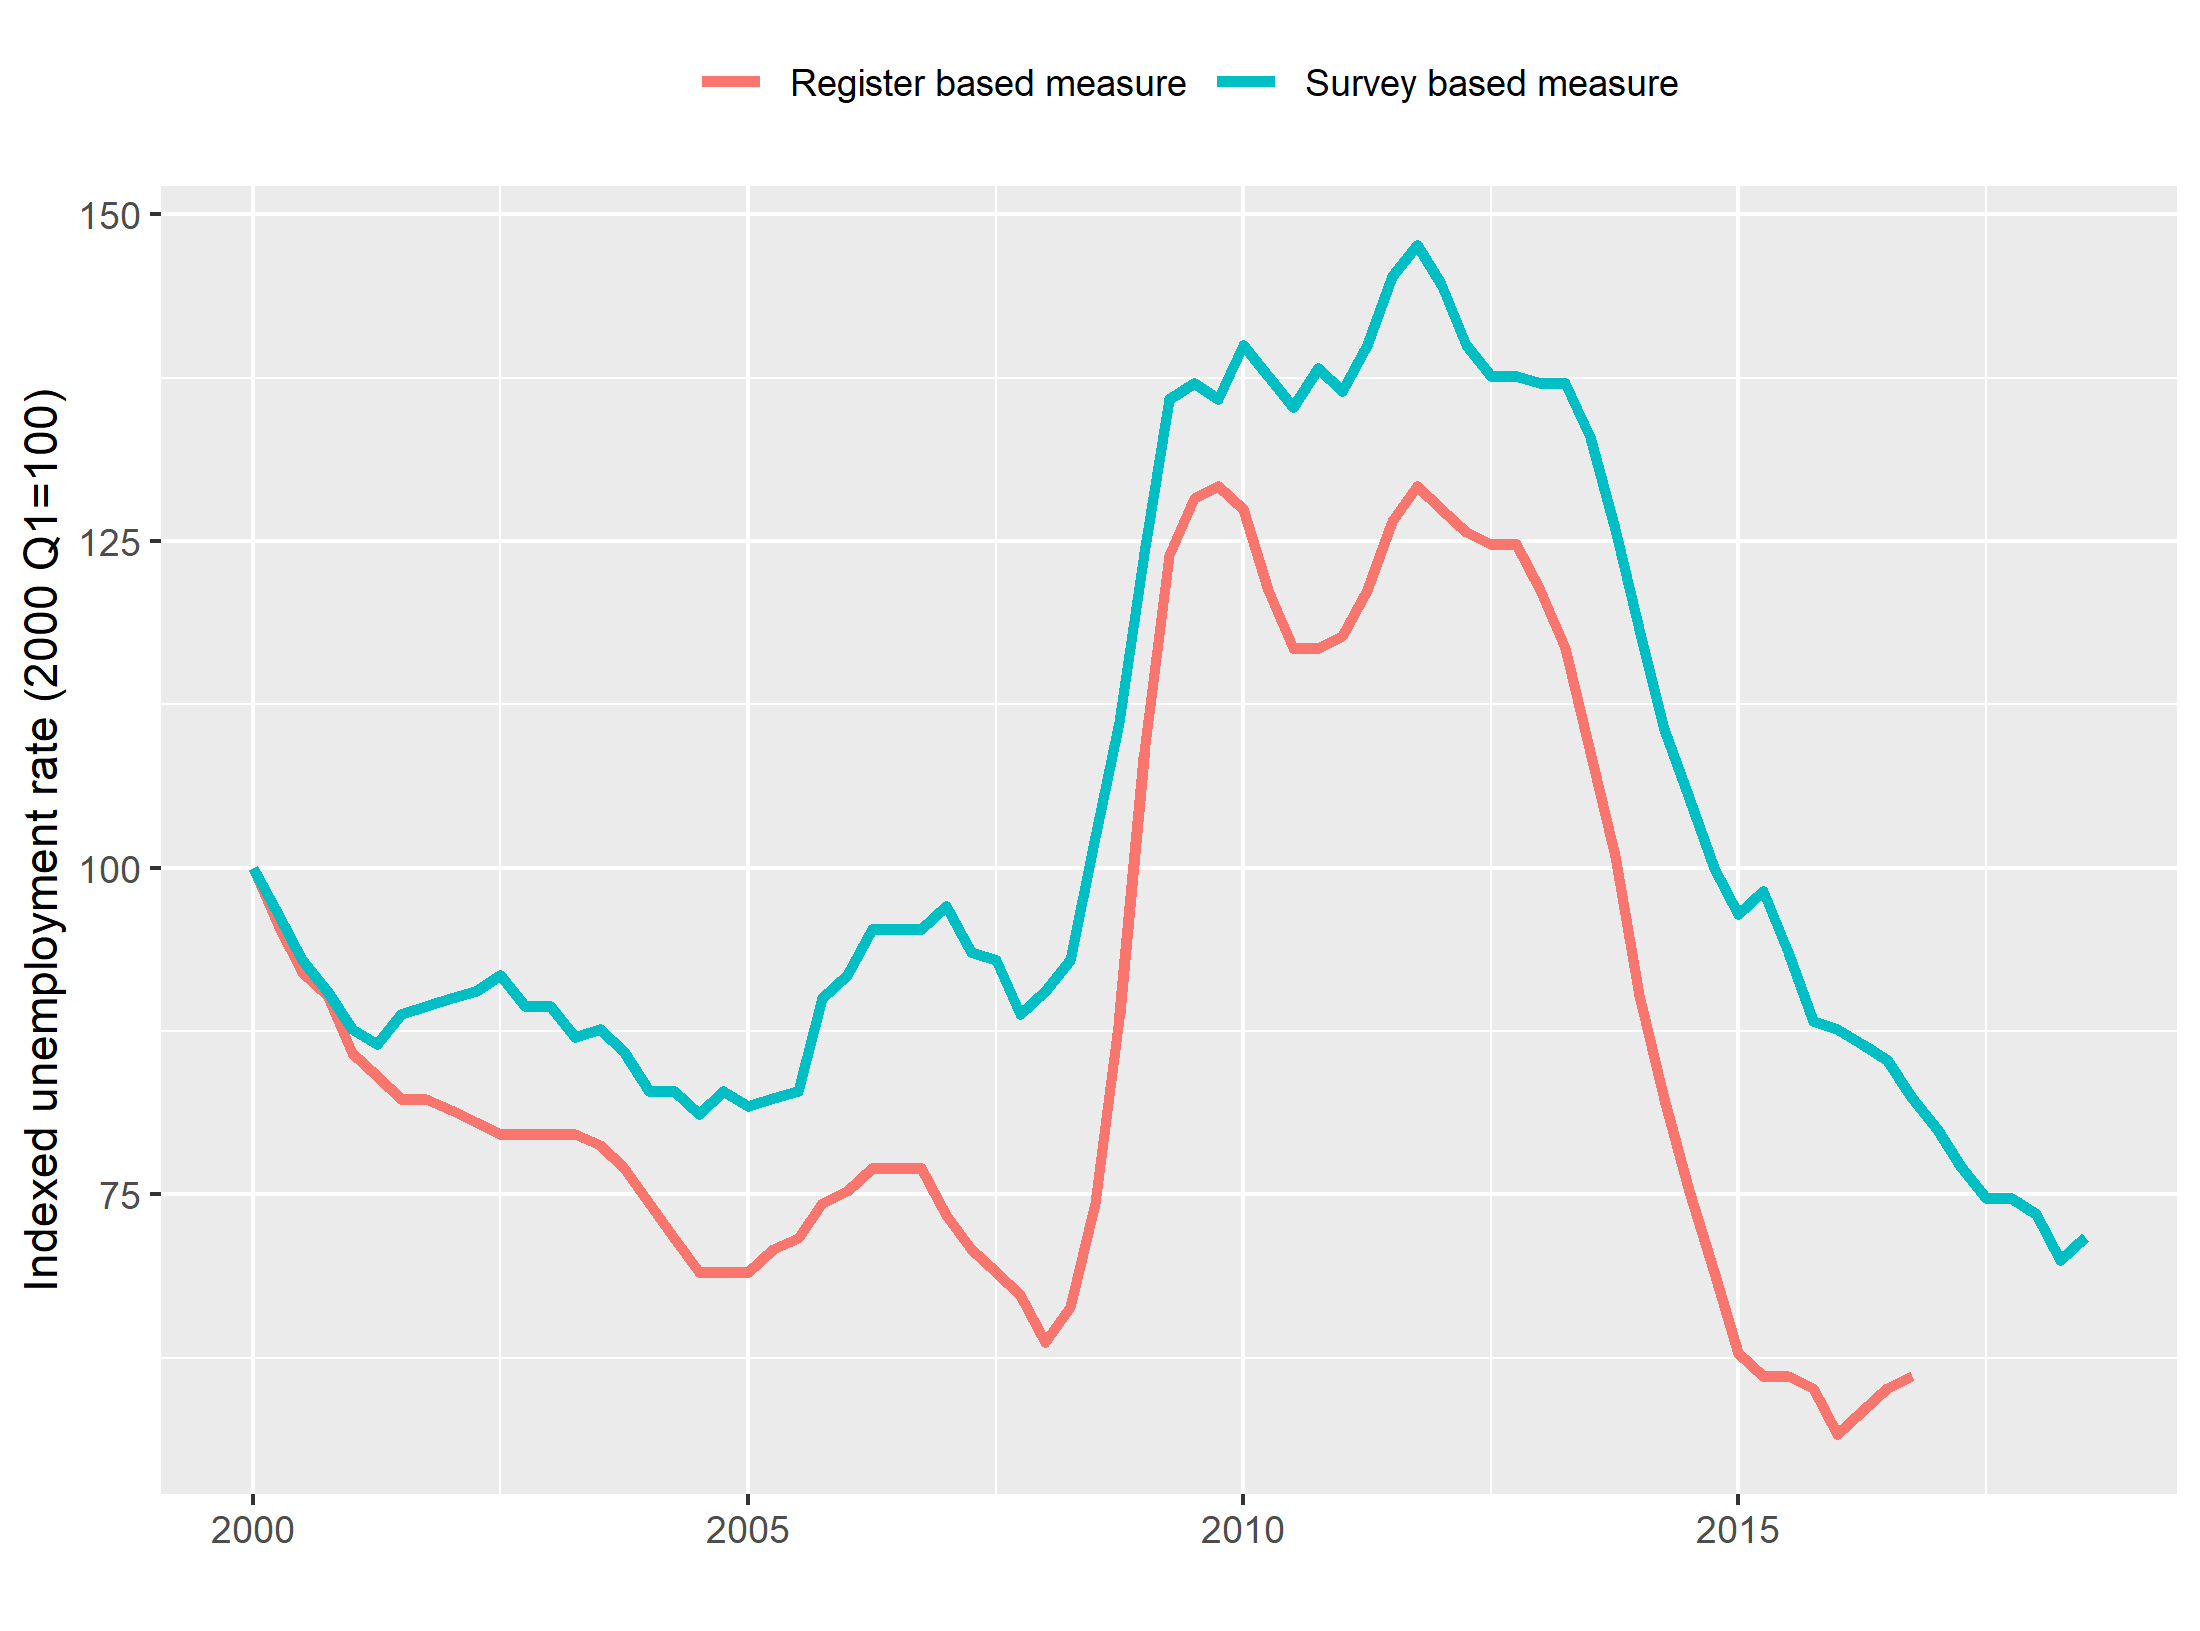
\includegraphics[width=0.49\linewidth]{_resources/chapter_labour/fig15}

\}

\textbackslash caption\{The unemployment rate in United Kingdom, using two different measures of unemployment. Data source: OECD. Left: in percent. Right: indexed to level in in Q1 2000=100. The R script for this Figure is available \href{https://www.hhsievertsen.net/economicdata/notes/lecture12/rmaterial/lecnote_12_script_for_fig8.R}{here}.\}\label{fig:labour2}
\textbackslash end\{figure\}

\hypertarget{out-of-the-labor-force}{%
\subsection{Out of the labor force}\label{out-of-the-labor-force}}

In the United Kingdom, the labor force is about half of the population (33 out of 66 million). What about the rest? First, there are children and individuals aged above 64. Then there are still about 8.9 million people left, where did they go? This group is called (economically) inactive by the Office for National Statistics. The inactivity rate is defined as follows:

\begin{align}
  \text{Inactive rate}=\frac{\text{Number of people aged 16 to 64 not in work/ available for work}}{\text{All people aged 16 to 64}}
\end{align}

So what do the ``economically inactive'' people do (or people who are not in the labor force, as I prefer to call them)? In the UK, the distribution of economically inactive is approximately as follows:

\begin{itemize}
\tightlist
\item
  27 percent are studying.
\item
  24 percent are looking after the family/staying home.
\item
  23 percent are long-term sick.
\item
  13 percent are retired.
\end{itemize}

Now that we have divided the population into groups according to their economic activity, we are ready to create graphs and tables on unemployment rate, employment rates and inactivity rates. However, there are a few useful concepts regarding seasonality and labor supply that are very useful to know before we start working with the data.

\begin{myblock}
\textbf{How to reduce the unemployment rates}

Imagine that you are working for a newly elected prime minister, and the
prime minister promised to lower unemployment rates, how could you
achieve this?

\begin{itemize}
\item
  Abandon the survey based measure of unemployment (the ILO measure),
  and only use the register based measure, because the latter tends to
  be lower.
\item
  Tighten the criteria for receiving unemployment benefits, as this will
  make less people receive benefits, which will lower the register based
  unemployment measure.
\item
  Introduce ``leave'' policies that allow unemployed workers to be ``on
  leave'' instead of unemployment. This will move people out of the
  unemployment category.
\end{itemize}

\emph{Are these policies good?}

\begin{itemize}
\tightlist
\item
  There might be normative arguments against and for these policies, but
  it is importantly: the immediate reduction in unemployment is caused
  by relabeling (or classification) of people, not by changing their
  actual situation.
\item
  (it might be that labeling people as ``unemployed'' or a leave policy
  affects the unemployment rate beyond the pure relabeling effect).
\end{itemize}
\end{myblock}

\hypertarget{labor-supply-extensive-vs.-intensive-margin}{%
\subsection{Labor supply: Extensive vs.~intensive margin}\label{labor-supply-extensive-vs.-intensive-margin}}

\hypertarget{what-about-the-intensive-margin}{%
\subsubsection{What about the intensive margin?}\label{what-about-the-intensive-margin}}

So far we have only discussed the extensive margin of the labor supply: whether people are working or not. However, labor supply is both a function of whether people work, and \emph{how much} they work. The former is called the \emph{extensive margin}, and the latter is called the \emph{intensive margin}. This distinction is useful in many cases. The extensive margin is typically a binary variable (to work or not), while the intensive margin is a continuous variable (how many minutes or hours of work). Recall from lecture note 4, how we could decompose changes in live births in changes in the general fertility rates and changes in the number of of women in childbearing ages. We could now use the same approach to decompose changes in labor supply in changes in how many people work, and changes in how many hours people on average work.

\hypertarget{policy-relevance-of-the-intensive-margin}{%
\subsubsection{Policy relevance of the intensive margin}\label{policy-relevance-of-the-intensive-margin}}

The distinction between extensive and intensive margin is important in many policy discussions. For example if we adjust tax policies, we might be interested in how it affects people's decision to join the labor market (the extensive margin) and people's decision on how much to work (the intensive margin).

\hypertarget{measuring-labor-supply-on-the-intensive-margin}{%
\subsubsection{Measuring labor supply on the intensive margin?}\label{measuring-labor-supply-on-the-intensive-margin}}

Measuring variation in intensive labor supply is slightly more challenging than measuring the extensive margin. I know that I work, but I have now precise idea about how many hours I work. For the United Kingdom, data on hours worked also comes from the Labour Force Survey. The Office for National Statistics makes the distinction between actual hours worked, average hours worked and the usual hours worked. They key difference is whether the measure is affected by absence (due to sickness or holiday).

\hypertarget{measuring-labor-supply-an-illustration-using-hours-worked.}{%
\subsubsection{Measuring labor supply: An illustration using hours worked.}\label{measuring-labor-supply-an-illustration-using-hours-worked.}}

In Figure \ref{fig:labour3}) we show the average weekly hours in the United Kingdom by gender compared to the European Union. The first observation we can make is that women have lower weekly hours than men. The second observation is that while the average weekly hours of men in the United Kingdom is slightly higher than the European Union 28 average, the average weekly hours of women is lower in the United Kingdom compared to the European Union 28.

\textbackslash begin\{figure\}

\{\centering 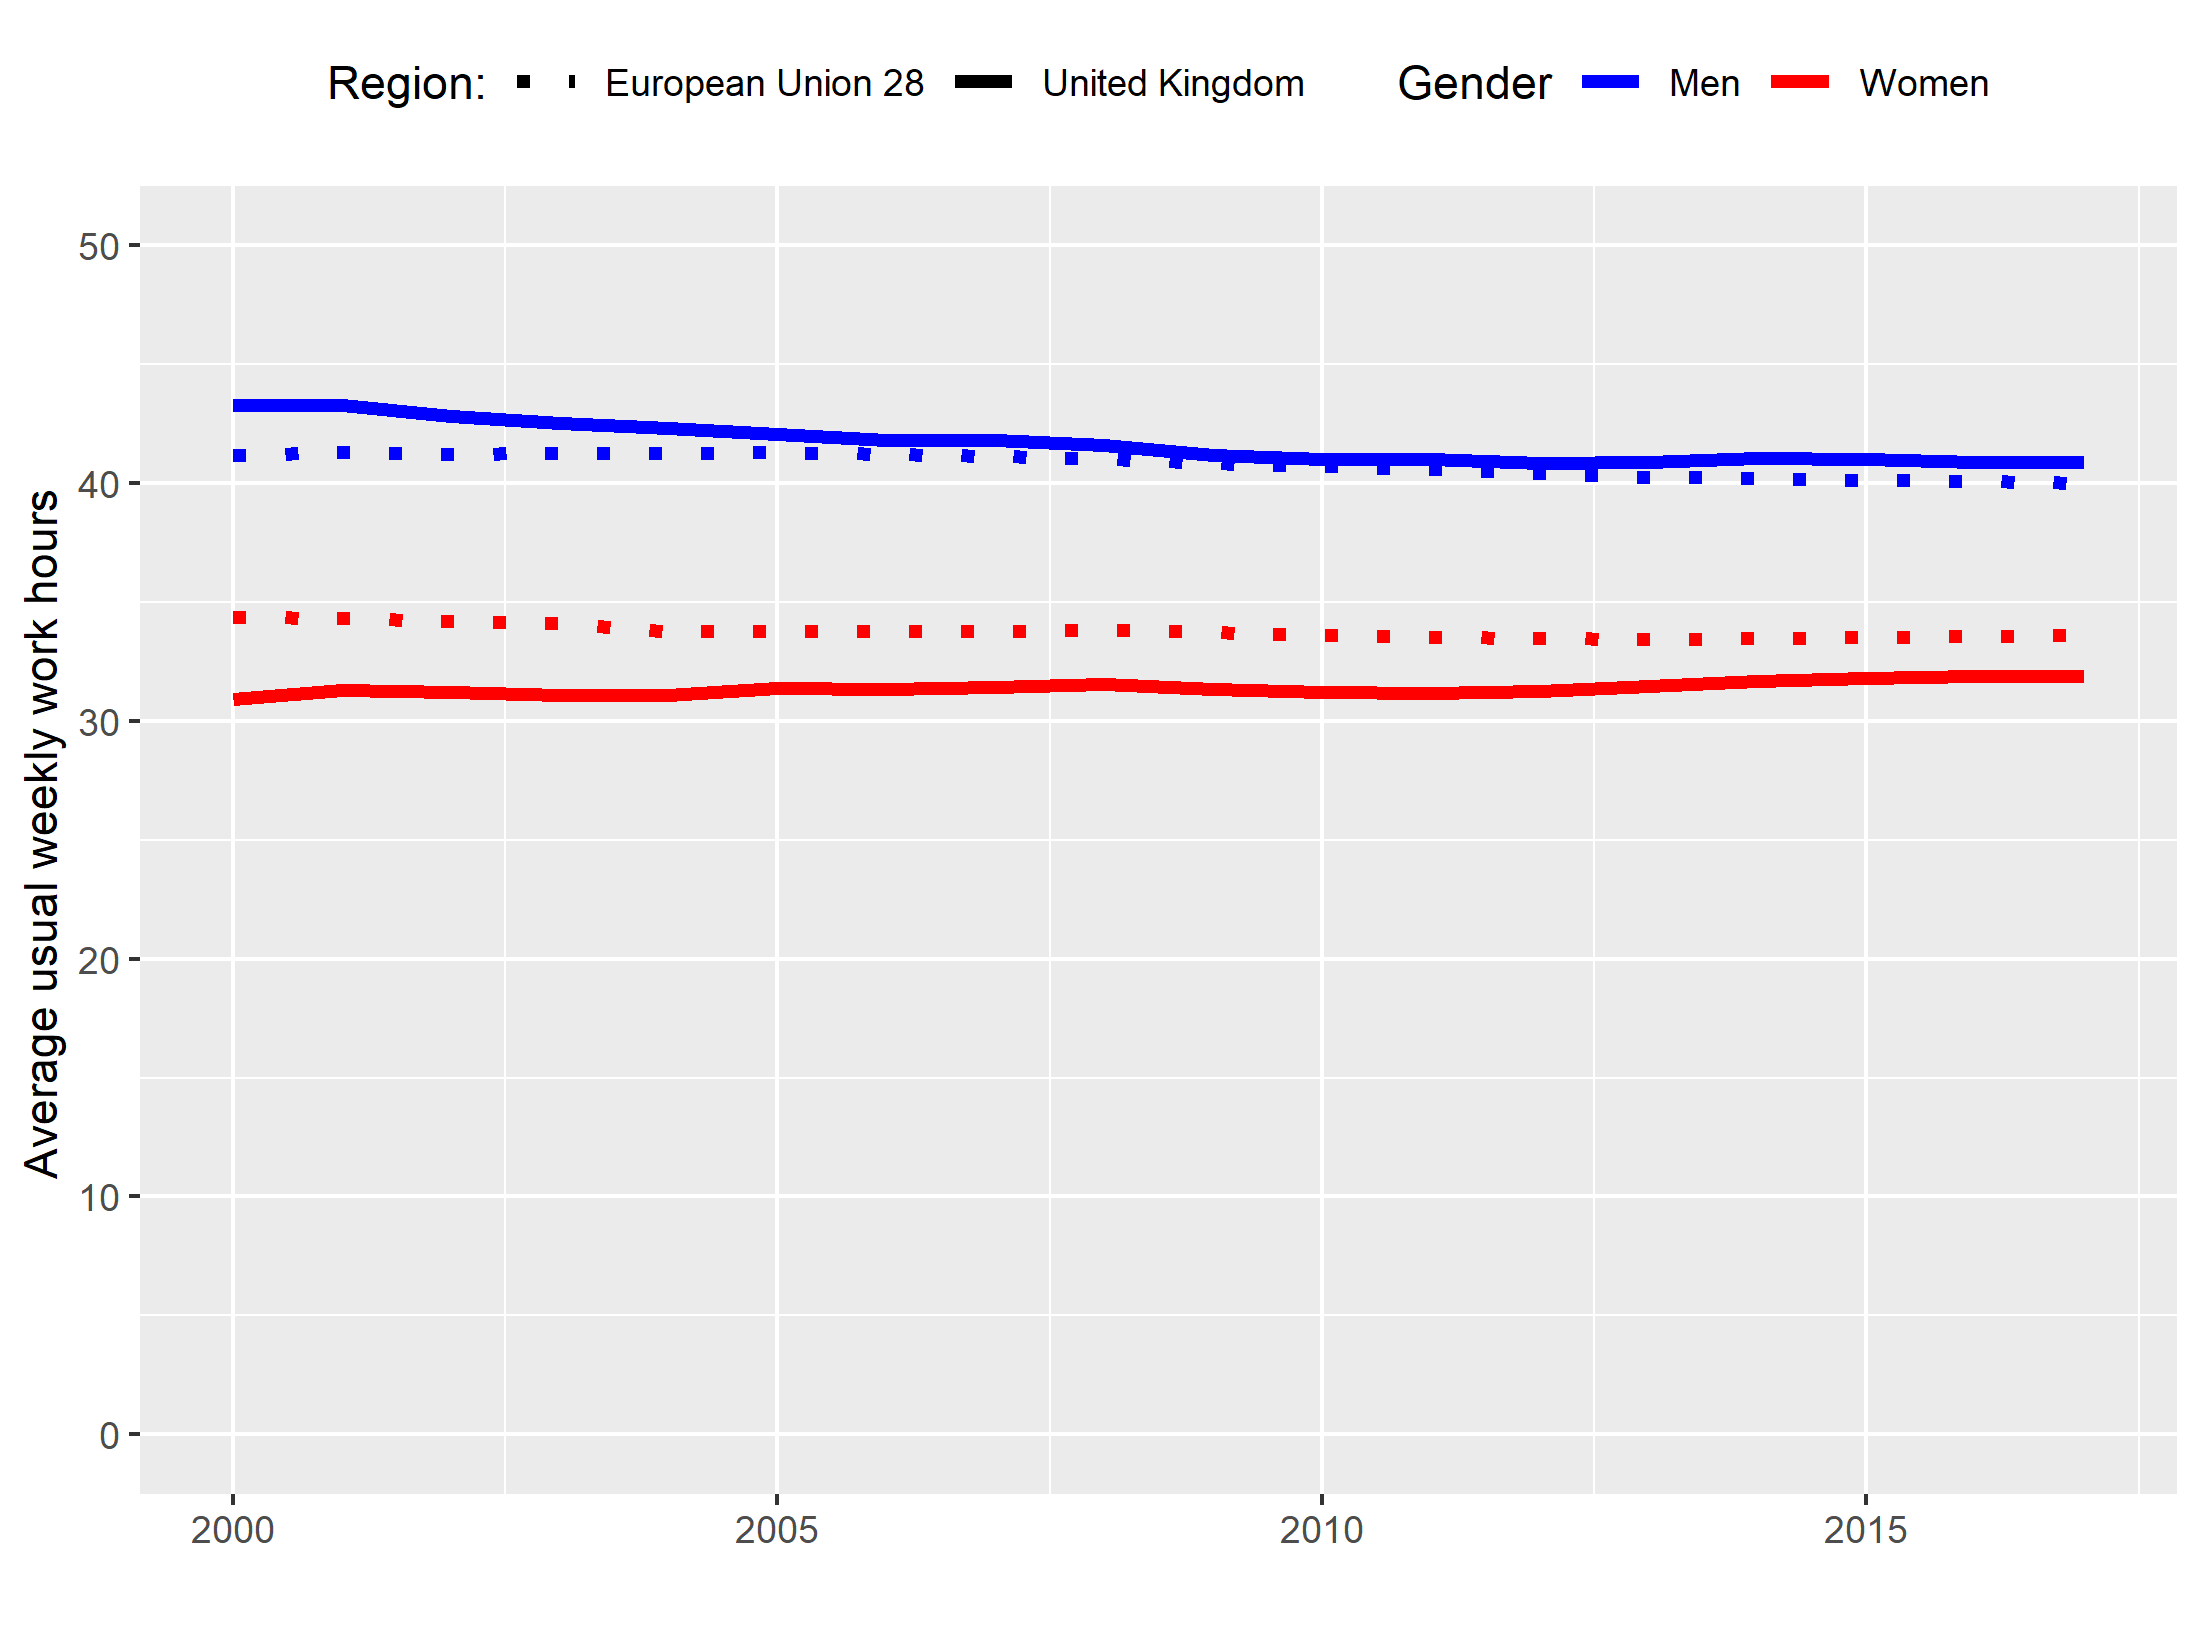
\includegraphics[width=0.89\linewidth]{_resources/chapter_labour/fig17}

\}

\textbackslash caption\{The intensive margin of labor supply: weekly hours worked in United Kingdom and the European Union 28. Data source: OECD. The R script for this Figure is available \href{https://www.hhsievertsen.net/economicdata/notes/lecture12/rmaterial/lecnote_12_script_for_fig9.R}{here}.\}\label{fig:labour3}
\textbackslash end\{figure\}

\hypertarget{the-demand-side-vacancies}{%
\section{The demand side: Vacancies}\label{the-demand-side-vacancies}}

\hypertarget{measuring-labor-demand}{%
\subsection{Measuring labor demand}\label{measuring-labor-demand}}

So far we only discussed the supply side of the labor market. The size of the labor force captures the potential supply of labor in an economy. But what about the demand side? How much labor is demanded in the economy? Measuring the demand size is challenging and considerably less standardized compared with the supply size. Just like for the labor supply side, there are two different sources of labor demand measures:

\begin{itemize}
\tightlist
\item
  Register based measures of labor demand: Using data from public employment services we can use the number of announced job vacancies as an indicator for labor demand.
\item
  Survey based measures: we can ask firms about their labor demand needs.
\end{itemize}

\hypertarget{advantages-and-disadvantages}{%
\subsubsection{Advantages and disadvantages}\label{advantages-and-disadvantages}}

These measures have advantages and disadvantages. The register based measure is considerably cheaper and tends to exist for longer periods and more countries. However, not all firms post their vacancies at the public employment service, so the sample of vacancies might not be representative of the actual number of vacancies. Moreover, the use of traditional job vacancy posting has changed over time, so this measure might be less representative today compared to what it used to be.

The survey based measure of vacancies on the hand is more expensive and suffers from the ``usual'' survey issues: not every firm responds and maybe the firms that respond are not representative. But compared to the register based measure, the ``non-representativeness'' might be less of a worry, although empirical evidence on this issue is not clear. As mentioned, the survey-based measure of job vacancies is less standardized than the survey-based measure of unemployment, but international organizations collect data on job vacancies and attempt to unify the definitions of job vacancies. The definition provided by Eurostat is as follows:

\begin{myblock}
\textbf{The Eurostat definition of a job vacancy}

According to the Eurostat job vacancy statistics a `vacancy' is defined
as a paid post that is newly created, unoccupied, or about to become
vacant:

\begin{itemize}
\item
  \begin{enumerate}
  \def\labelenumi{(\alph{enumi})}
  \tightlist
  \item
    for which the employer is taking active steps and is prepared to
    take further steps to find a suitable candidate from outside the
    enterprise concerned; and
  \end{enumerate}
\item
  \begin{enumerate}
  \def\labelenumi{(\alph{enumi})}
  \setcounter{enumi}{1}
  \tightlist
  \item
    which the employer intends to fill either immediately or within a
    specific period of time.
  \end{enumerate}
\end{itemize}

For more details, see the source:
\url{https://ec.europa.eu/eurostat/cache/metadata/en/jvs_esms.htm}
\end{myblock}

\hypertarget{the-job-vacancy-rate}{%
\subsubsection{The job vacancy rate}\label{the-job-vacancy-rate}}

We can relate the number of vacancies to the size of the labor force to obtain a measure of the job vacancy rate. While this is the typically textbook measure of the job vacancy rate \citep[p.~512 in][]{zyb}, statistical databases often provide slightly different measures. Eurostat defines the job vacancy rate as follows:

\begin{align}
  \text{JVR}_{\text{Eurostat}}=\frac{\text{number of vacancies}}{\text{number of occupied posts}+\text{number of vacancies}}
\end{align}

If we are willing to approximate the number of occupied posts by the number of employed people, the main difference between these two definitions of the job vacancy rate is whether we include vacancies or unemployment in the denominator. Both measures are commonly used, but it is of course important to be consist when comparing job vacancy rates across regions and time. A reduction in vacancies will lead to a smaller reduction in the job vacancy rate using the Eurostat definition that the \citep{zyb} definition, because in the latter it only affects the numerator.

\hypertarget{supply-meets-demand}{%
\section{Supply meets demand}\label{supply-meets-demand}}

We can combine our measures of labor supply and demand to create the Beveridge Curve, which is named after its ``inventor'', the English economist William Beveridge. The Beveridge curve shows the job vacancy rate on the vertical axis against the unemployment rate on the horizontal axis. The Beveridge curve is a simple indicator of the matching efficiency of the labor market. Without any frictions and in the simples economic model, the graph should only ``exist'' on the axes: We should only have a positive job vacancy rate if unemployment is zero, and we should only have unemployment if we have no vacancies. In practice, this is clearly not the case as Figure x shows. We have unemployment and vacancies at the same time. How can that be and how does that say something about the labor market?

\begin{itemize}
\item
  The unemployed worker and the vacancy haven't ``matched'' yet: search frictions and other difficulties mean that even if there is a suitable unemployed candidate, the open position might not be filled immediately. There is an application deadline, formal procedures and the unemployed first has to find the job.
\item
  An outward shift in the Beveridge curve (as illustrated) suggests a reduction in the matching efficiency of the labor market: For a given number of vacancies in the economy, we have a higher a unemployment rate.
\item
  However, there are other reasons for shifts in the labor market than pure search frictions.
\item
  The assumptions of a homogeneous labor market is very simplified.
\item
  There might be vacancies in Manchester and the unemployed in London (geographical mismatch)
\item
  There might be firms looking for lawyers, but only unemployed economists (skill mis-match).
\item
  and so on.
\end{itemize}

\textbackslash begin\{figure\}

\{\centering 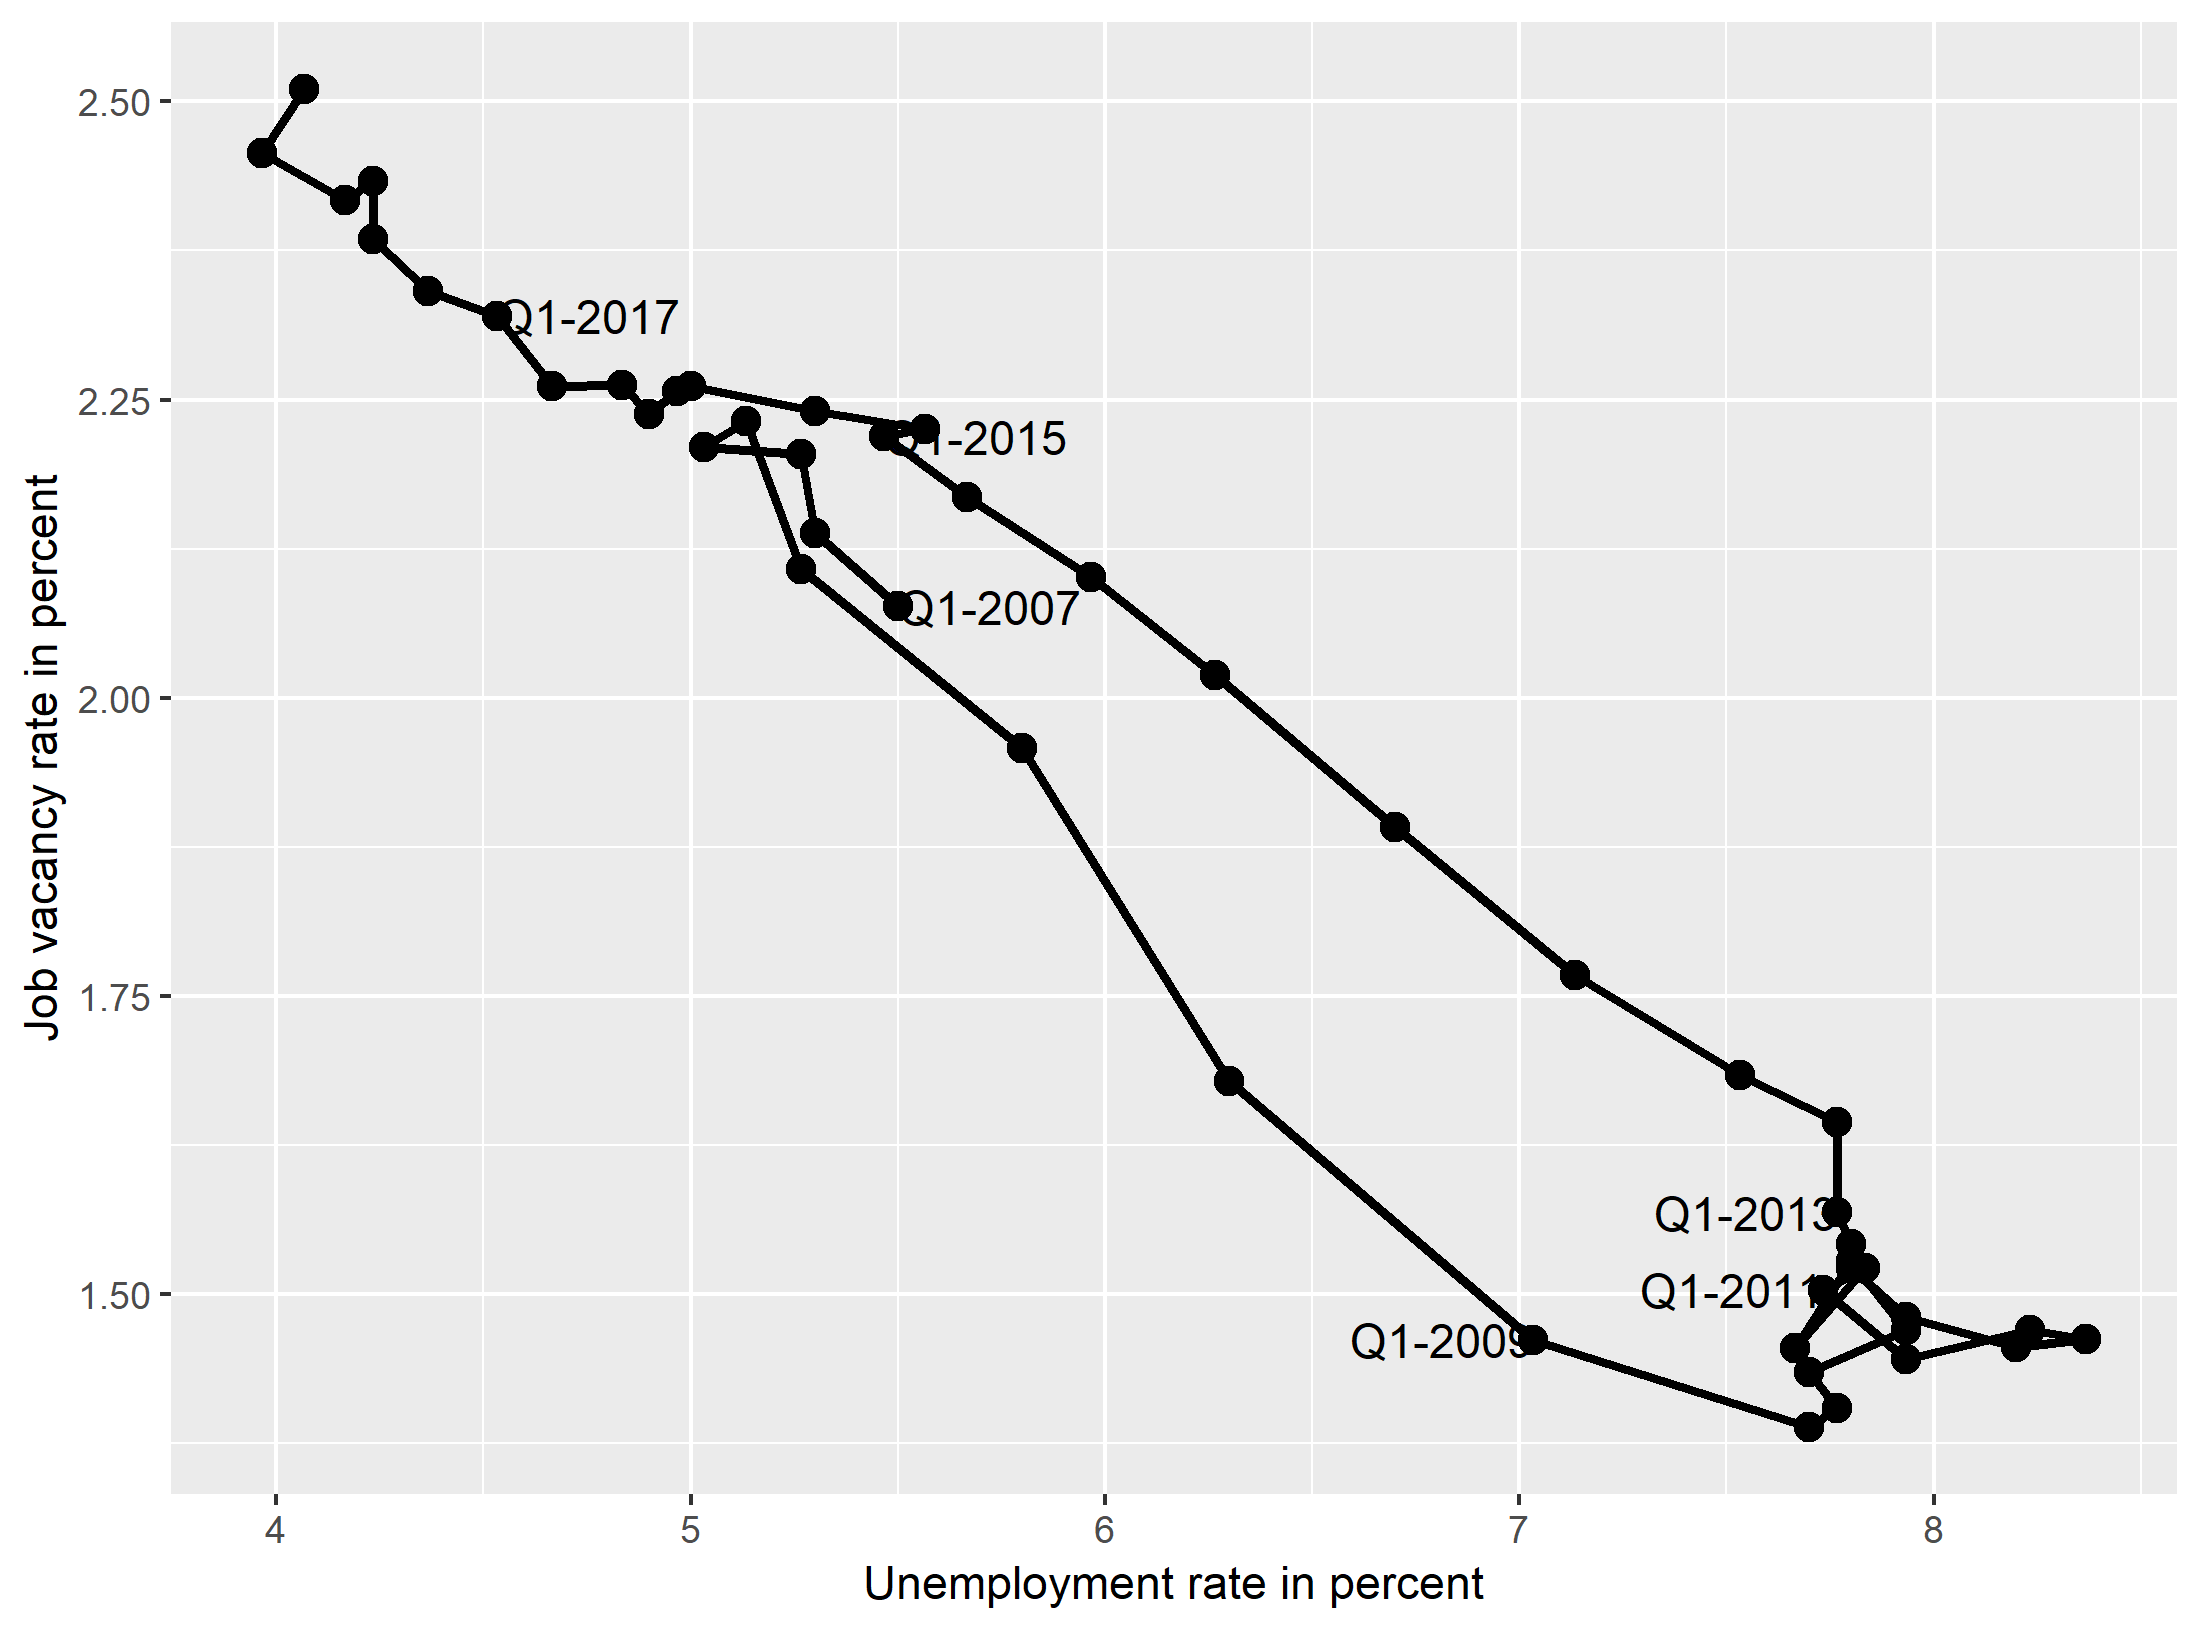
\includegraphics[width=0.89\linewidth]{_resources/chapter_labour/fig16}

\}

\textbackslash caption\{The Beveridge curve for the United Kingdom. Data source: OECD. The R script for this Figure is available here \href{https://www.hhsievertsen.net/economicdata/notes/lecture12/rmaterial/lecnote_12_script_for_fig10.R}{here}.\}\label{fig:labour4}
\textbackslash end\{figure\}

\hypertarget{summary-5}{%
\section{Summary}\label{summary-5}}

In this lecture we have covered the following topics:

\begin{itemize}
\tightlist
\item
  Definitions of unemployment rates:

  \begin{itemize}
  \tightlist
  \item
    The survey based measure of unemployment.
  \item
    The register based measure of unemployment.
  \end{itemize}
\item
  The extensive and intensive margin of labor supply.
\item
  Labor demand and the Beveridge curve.
\end{itemize}

\hypertarget{measuring-inequality}{%
\chapter{Measuring inequality}\label{measuring-inequality}}

\hypertarget{about-this-chapter-6}{%
\section{About this chapter}\label{about-this-chapter-6}}

One of the criticisms of GDP as a well-being measure is that ``GDP ignores the distribution'' (see chapter x). GDP is simply an average across the entire economy. It doesn't tell us who experiences the ``economic activity'', beyond the decomposition into sectors or workers and firms. If we look behind these total numbers and consider the \emph{distribution} of the income, we would probably see something like the chart shown in Figure \ref{fig:in0}. The chart is a histogram of income for a simulated income. Most individuals earn an income well below 100 thousand pounds per year, but some earn way more than that. This chapter is about how we can describe such patterns and compare them across countries and across time.

\begin{figure}

{\centering 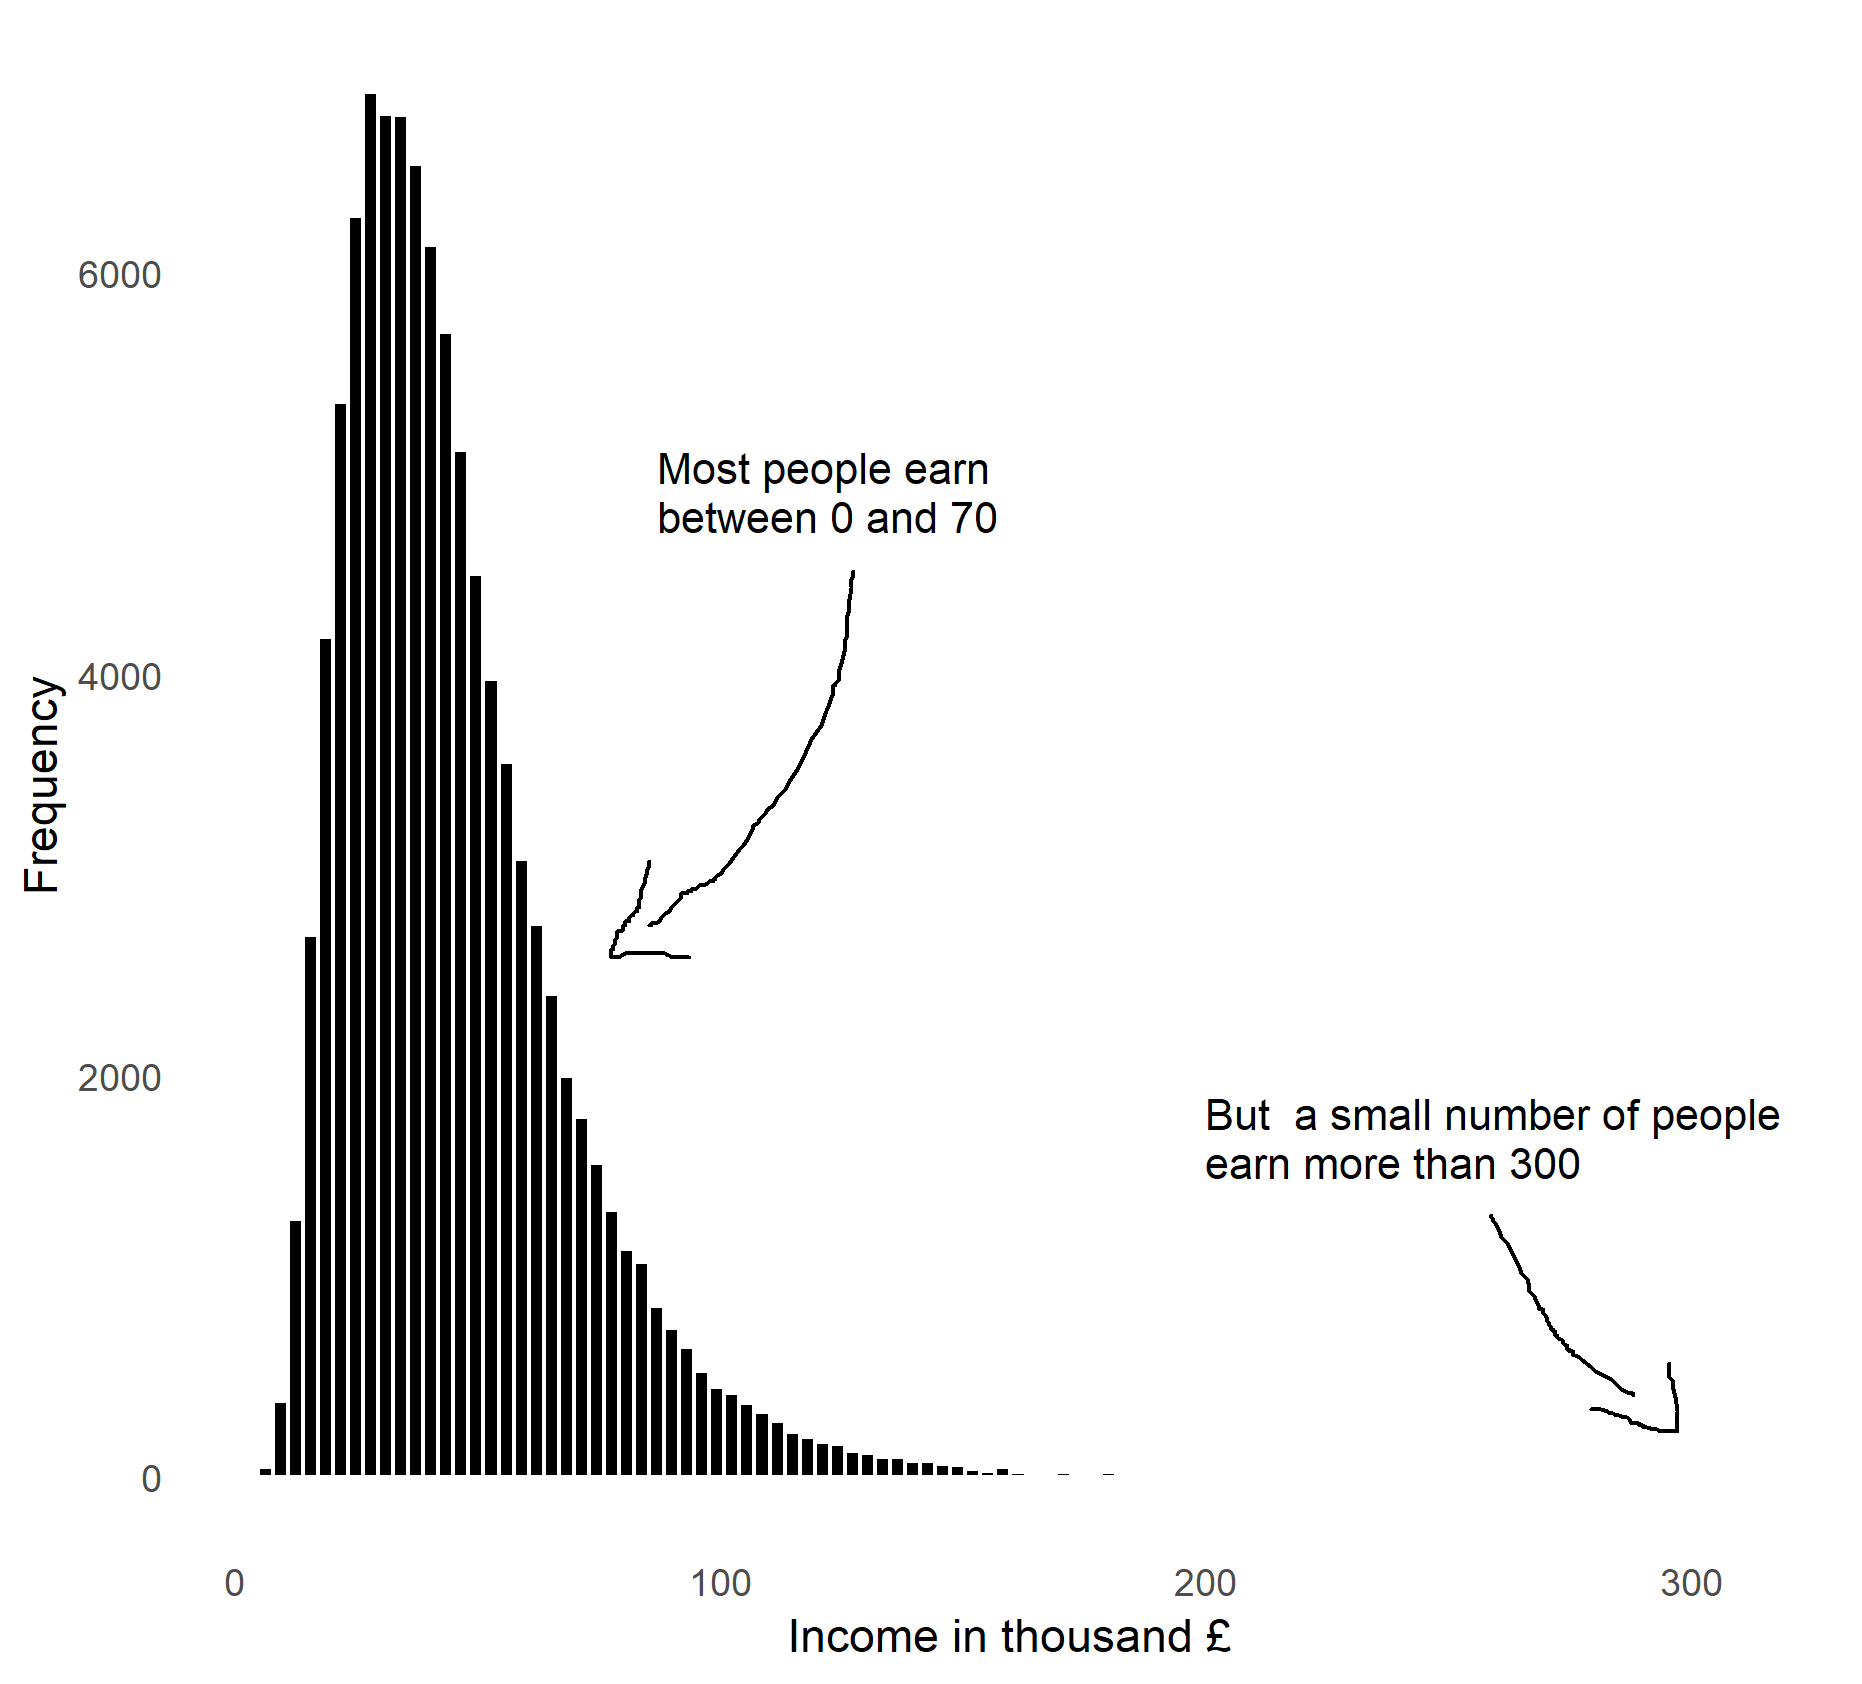
\includegraphics[width=0.85\linewidth]{_resources/chapter_inequality/hist2} 

}

\caption{The distribution of income. Data is simulated.}\label{fig:in0}
\end{figure}

\hypertarget{intended-learning-outcomes-5}{%
\subsection{Intended learning outcomes}\label{intended-learning-outcomes-5}}

After reading this chapter you should be able to

\begin{itemize}
\tightlist
\item
  Explain the difference between macro and micro level data.
\item
  Explain the data requirements for studying income or wealth inequality.
\item
  Create histograms and compute income shares
\item
  Create a Lorenz curve
\item
  Calculate and interpret the Gini coefficient
\end{itemize}

\hypertarget{data-requirements-1}{%
\section{Data requirements}\label{data-requirements-1}}

\hypertarget{macro-and-micro-level-data}{%
\subsection{Macro and micro level data}\label{macro-and-micro-level-data}}

\hypertarget{macro-level-data}{%
\subsubsection*{Macro level data}\label{macro-level-data}}
\addcontentsline{toc}{subsubsection}{Macro level data}

So far we've mostly been using macro level data. Macro level data is data about countries, regions or other entities comprising many individuals, households, firms and institutions. An observation in macro data represents the average, the sum or another statistic of these individuals, firms and institutions. We can typically download most macro data from a public source.

\hypertarget{micro-level-data}{%
\subsubsection*{Micro level data}\label{micro-level-data}}
\addcontentsline{toc}{subsubsection}{Micro level data}

In micro level data each observation represents the value for an individual, a household, a firm or an institution. Micro data is often the basis for macro data. It is often based on surveys or administrative records. Micro data is rarely directly accessible from public sources. One reason for this is that micro data often contains a lot of detailed information that shouldn't be shared freely with everyone. Getting access to micro data therefore often requires us to submit an application and sign a confidentiality agreement. Moreover, when working with micro level data we should be careful with how we share and store the data.

Because I cannot share of the micro level data I have publicly, the data in \ref{fig:in0} is simulated. I created the data in R, using the following comands:\footnote{I also made some minor adjustments to improve the data to ink ratio and make the chart self-explanatory. You should try that yourself.}

\begin{Shaded}
\begin{Highlighting}[]
\KeywordTok{library}\NormalTok{(tidyverse)}
\NormalTok{df<-}\KeywordTok{tibble}\NormalTok{(}\DataTypeTok{income=}\KeywordTok{exp}\NormalTok{(}\KeywordTok{rnorm}\NormalTok{(}\DecValTok{100000}\NormalTok{,}\KeywordTok{log}\NormalTok{(}\DecValTok{40}\NormalTok{),}\FloatTok{0.5}\NormalTok{)))}
\KeywordTok{ggplot}\NormalTok{(}\DataTypeTok{data=}\NormalTok{df,}\KeywordTok{aes}\NormalTok{(}\DataTypeTok{x=}\NormalTok{income)) }\OperatorTok{+}\StringTok{ }
\StringTok{  }\KeywordTok{geom_histogram}\NormalTok{( }\DataTypeTok{bins=}\DecValTok{100}\NormalTok{,}\DataTypeTok{fill=}\StringTok{"black"}\NormalTok{, }\DataTypeTok{col=}\StringTok{"white"}\NormalTok{)}
\end{Highlighting}
\end{Shaded}

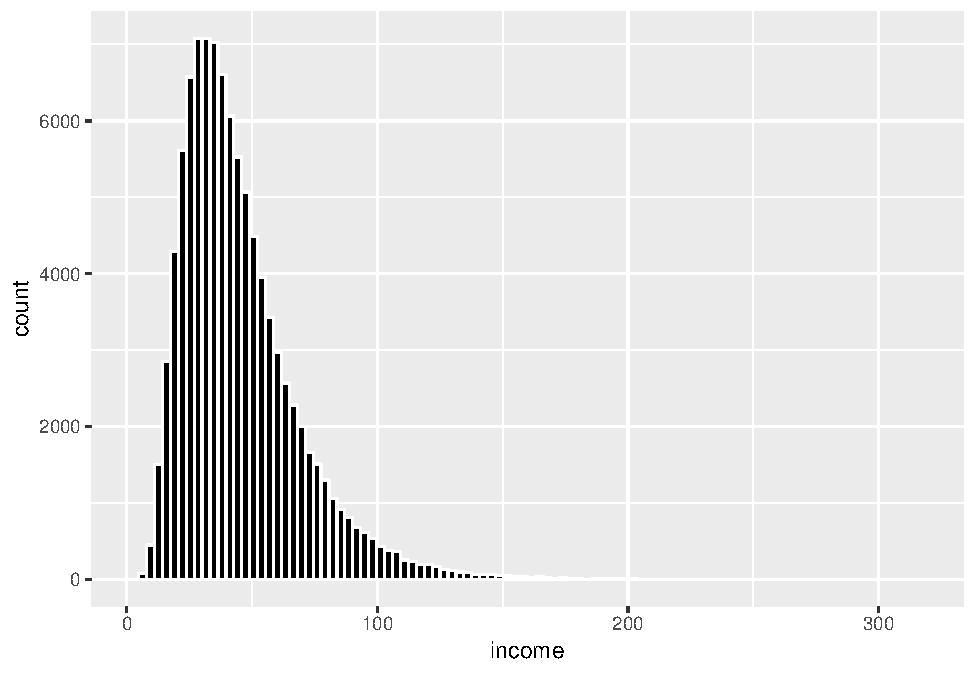
\includegraphics{book_files/figure-latex/unnamed-chunk-21-1.pdf}

\hypertarget{net-and-gross-values}{%
\subsection{Net and gross values}\label{net-and-gross-values}}

When assessing the distribution of income within the population it is important first to decide whether we are interested in the net or gross income distribution. We've already used the term ``net'' and ``gross'' on several occasions. When discussing net-migration or Gross Domestic Product. But what do these terms mean? In general we can think of the terms net and gross as follows:

\begin{itemize}
\tightlist
\item
  Gross: The value without deductions, contributions etc.
\item
  Net: The value after deductions, contributions etc.
\end{itemize}

We use the terms net and gross in many situations. If you buy packaged food the label might display the gross and net weight. The gross weight will then be the total weight before deductions, the net weight will be the weight of the product after we deducted the weight of the packaging etc.

The most common use of the terms net and gross is probably in income, where gross refers to the income before taxes, and net to the income after taxes. Statistical offices and economists in general agree on excluding taxes from gross terms and including taxes in net terms, but there is less agreement on whether transfers such as housing benefits and unemployment benefits in net terms should be included.

When working with income data, the concept of disposable income is therefore also often used instead. The idea is that we want to consider the income that the household can spend, which will be the income after all taxes, transfers, and deductions.

\hypertarget{equivalenced-income}{%
\subsection{Equivalenced income}\label{equivalenced-income}}

In working with income data we are often interested in comparing households instead of individuals. However, households are not all of the same size, and we will therefore have to adjust monetary measures to the size of the households, we call income that is adjusted to household equivalenced income. We will here briefly discuss the three most common approaches to equivalise income.

\begin{itemize}
\item
  The Oxford scale or OECD equivalence scale.

  \begin{itemize}
  \tightlist
  \item
    The first person in the household: Weight 1
  \item
    Each additional adult household member: Weight 0.7 (person aged 14 and over)
  \item
    Each child household member: Weight 0.5
  \end{itemize}
\item
  The OECD modified scale.

  \begin{itemize}
  \tightlist
  \item
    The first person in the household: Weight 1
  \item
    Each additional adult household member: Weight 0.5 (person aged 14 and over)
  \item
    Each child household member: Weight 0.3
  \end{itemize}
\item
  The Square root scale.

  \begin{itemize}
  \tightlist
  \item
    Total weight: square root of the number of household members.
  \end{itemize}
\end{itemize}

While the square root method is probably the most popular approach, the choice of approach is non-trivial as Table \ref{tab:povt0} shows. The table shows four different households that all have the same income, but the composition of households vary. The Oxford scale does for example but quite high weight on children compared to the modified OECD scale. The square root scale on the other hand puts the same weight on adults and children, but each additional member gets a lower weight.

\begin{longtable}[]{@{}lcccc@{}}
\caption{\label{tab:povt0} Equivalencing income}\tabularnewline
\toprule
Adults & 1 & 2 & 1 & 2\tabularnewline
\midrule
\endfirsthead
\toprule
Adults & 1 & 2 & 1 & 2\tabularnewline
\midrule
\endhead
Children & 0 & 0 & 1 & 2\tabularnewline
Household income & 100 & 100 & 100 & 100\tabularnewline
Equivalised income & & & &\tabularnewline
Oxford scale & 100 & 58.824 & 66.667 & 37.037\tabularnewline
OECD modified & 100 & 66.667 & 76.923 & 47.619\tabularnewline
Square root & 100 & 70.711 & 70.711 & 50.000\tabularnewline
\bottomrule
\end{longtable}

When working with household income data you should adjust income measures and be aware of the differences between the approaches.

\hypertarget{a-histogram}{%
\subsection*{A histogram}\label{a-histogram}}
\addcontentsline{toc}{subsection}{A histogram}

While most data representation tools are concerned with the relationship between two or more variables, histograms focus on only one variable; they are used to show the \emph{distribution} of a single variable\}. Histograms look very much like bar charts, and one interpretation of a histogram is, that it is a special case of a bar chart, where the x-axis is always showing intervals of the variable. Another peculiarity of a histogram is that y-axis typically shows the \emph{density}.

To create a histogram we conduct the following steps:

\begin{enumerate}
\def\labelenumi{\arabic{enumi}.}
\tightlist
\item
  Decide on the categories used on the x-axis.
\item
  Count the number frequencies of each category selected in step 1.
\item
  Convert the counts to relative frequencies (optional).
\end{enumerate}

The first step seems very trivial. However, often the data is not discrete and the categories on the x-axis will be intervals. When values are continuous we will have to group a range of values in a \emph{bin}. For example a bin containing all values between 1 and 2 (i.e.~1, 1.00001, 1.0004,1.431 etc.). The choice of bins is actually quite important. There is a trade-off between getting a more smooth picture of the distribution (i.e.~with coarse bins) and getting a detailed but more noisy picture of the distribution (i.e.~with fine bins).

\hypertarget{selecting-the-bin-width}{%
\subsubsection*{Selecting the bin width?}\label{selecting-the-bin-width}}
\addcontentsline{toc}{subsubsection}{Selecting the bin width?}

So how do we select bin widths? Notice that we can \emph{either} make a choice of the number of bins \emph{or} make a choice of the bin widths. As these two are related we cannot select them independently. In practice, the choice of the number of bins (or bin width) is rather ad hoc. However, most statistical software has built in ``rule-of-thumb'' decision rules. Let us briefly discuss some of the basic rules. Let \emph{k} be the number of bins, we can select \emph{k} based on:

\begin{itemize}
\item
  The square root rule

  \begin{align}
        k=\sqrt(N)
    \end{align}
\end{itemize}

where \emph{N} is the number of observations.

\begin{itemize}
\tightlist
\item
  Stata's default
  \begin{align}
        k=\min\left\{\sqrt(N), \frac{10\ln(N)}{\ln(10)}\right\}
    \end{align}
\end{itemize}

such that \emph{k} is the lowest value of the square root rule and ten times the natural logarithm of the number of observations divided by the natural logarithm of ten.

\begin{itemize}
\tightlist
\item
  Sturges' rule
  \begin{align}
        k=log_2(N)+1
    \end{align}
\end{itemize}

this formula is used as the default in R (Base). With 2000 observations Sturges's rule suggest 12 bins.

Note how the three different formulas provided very different suggestions. The same data will lead to bar chart with 12 bins in R and 33 bins in Stata. It is therefore always a good idea to assess the histogram using various bin specifications, manually.

\hypertarget{what-are-densities}{%
\subsubsection*{What are densities?}\label{what-are-densities}}
\addcontentsline{toc}{subsubsection}{What are densities?}

In the histograms we've plotted so far, the y-axis has always shown relative frequencies. However, often the y-axis of histogram shows something called densities. In practice there are three options for the y-axis:

\begin{itemize}
\tightlist
\item
  Counts: i.e.~the frequency.
\item
  Relative frequency (the frequency divided by the number of data points)
\item
  Frequency density (the frequency relative to the bin width) or the Probability density.
\end{itemize}

The frequency density is the frequency divided by the bin width, and the probability density is the relative share divided with the bin width.

\hypertarget{income-shares}{%
\section{Income shares}\label{income-shares}}

How can we summarise distribution shown in Figure \ref{fig:in0} in a measure of inequality? If we share a cake among four friends, we would evaluate whether the distribution of cake by assessing whether everyone had an equal share of the cake. Everyone should have 25 percent of the cake. We can conduct a similar exercise with income. Let's first try this on the simulated example from above:

\begin{figure}

{\centering \includegraphics{book_files/figure-latex/inx1-1} 

}

\caption{\label{fig:figx} Income shares based on simulated data.}\label{fig:inx1}
\end{figure}

\hypertarget{income-or-wealth}{%
\subsection{Income or wealth}\label{income-or-wealth}}

When talking about inequality it is important to be precise about what dimension of inequality we are interested in. The two most commonly assessed dimensions are income and wealth. Wealth inequality is typically higher than income inequality. We could also assess inequality with respect to other dimensions, such as mortality, social activites, etc.

What does this chart show us? On the horizontal axis we have the income percentile. On the vertical axis we have the the income share. The percentile is based on the income rank. Percentile 1 contains the 1 percent of the observations with the lowest income. Percentile 100 contains the 1 percent of the population with the highest income.

From this chart we see that the 1 percent with the lowest income has a total income well of around 0.25 percent of the total income. The 1 percent with the highest income has more than 3 percent of total income. In the cake example we split the cake in four and an equal distribution is then that everyone has one-fourth of the total cake. In the sample above we do the same, but we split income in 100 percentiles instead of four. An equal distribution would be a situation where every percentile has 1-100 of the total income. In other words everyone should have 1 percent. But this is not the case. The richest 1 percent have more than 3 times their equal share. The poorest 1 have about one-fourth of their equal share. Let's try to look at some real data.The We don't have access to individual level income data, but several data sources provide processed income data on income. The following example uses data from the \href{https://wid.world/data/}{World Inequality Database}.

\begin{verbatim}
## Warning: Removed 2 rows containing missing values (geom_path).
\end{verbatim}

\begin{figure}

{\centering \includegraphics{book_files/figure-latex/inx2-1} 

}

\caption{\label{fig:figx1} Income shares in the UK. Data source: World Inequality database}\label{fig:inx2}
\end{figure}

So what does this chart tell us? We can see that the in early 1980ies, the top 1 percent (the p99p100) had about seven percent of the total income in the UK. That is about 7 times more than their equal share. In 2012 that share was about 12 percent. The income share of the top 1 percent has increased and almost doubled over the last three decades.

Where did that increase in income to the top 1 percent come from? The red line in the chart shows the income share of the bottom 50 percent. This group had about 24 of the total income in the early 1980ies. That is about half of their equal share. Over the three decades their income share dropped by about 2.5 percentage points. Part of the increase in the top income share is therefore from the bottom 50 percent, but not everything.

We have now introduced already used our first measures of inequality:

\begin{itemize}
\tightlist
\item
  the income share of the top 1 percent.
\item
  the income share of the bottom 50 percent.
\end{itemize}

\hypertarget{the-lorenz-curve-and-the-gini-coefficient}{%
\section{The Lorenz curve and the Gini coefficient}\label{the-lorenz-curve-and-the-gini-coefficient}}

So far, we have looked at specific parts of the income distribution. What about the other parts of the income distribution and their income shares? And can we combine all these income shares in one measure? Yes, that is what the Lorenz curve does

One of the most common approaches to show income distributions is the Lorenz-curve, developed by the American economist, Max Lorenz. The curve plots the share of total income relative to the position in the income distribution. So on the x-axis we rank the population by their income and on the y-axis we show the cumulative income share. Here is cookbook for creating a Lorenz curve:

\begin{enumerate}
\def\labelenumi{\arabic{enumi}.}
\item
  Sort all households (individuals) by their income, from lowest to highest and give them a relative income rank.
\item
  Compute the total income in the population.
\item
  For each individual in the household calculate their share of total income.
\item
  Calculate the cumulative income share by adding the individual shares. So for the household with the lowest income, the cumulative share is just their income share. For the second lowest income household, the cumulative income share is their share plus the share of the lowest income household.
\item
  Create a line chart of the cumulative income shares against the household (individual) income rank.
\end{enumerate}

Now what do we expect? How does this chart look? Let's consider a very simple example of an economy with 10 households as shown in Table \ref{tab:povt1}. In scenario 1 all households have the same income. In scenario 2, one household has all income of the economy. In scenario 3 the income is gradually increasing.

\begin{longtable}[]{@{}cccc@{}}
\caption{\label{tab:povt1} 3 examples of distributions}\tabularnewline
\toprule
Household & Scenario 1 & Scenario 2 & Scenario 3\tabularnewline
\midrule
\endfirsthead
\toprule
Household & Scenario 1 & Scenario 2 & Scenario 3\tabularnewline
\midrule
\endhead
1 & 10 & 0 & 3\tabularnewline
2 & 10 & 0 & 5\tabularnewline
3 & 10 & 0 & 6\tabularnewline
4 & 10 & 0 & 8\tabularnewline
5 & 10 & 0 & 9\tabularnewline
6 & 10 & 0 & 10\tabularnewline
7 & 10 & 0 & 12\tabularnewline
8 & 10 & 0 & 13\tabularnewline
9 & 10 & 0 & 14\tabularnewline
10 & 10 & 100 & 30\tabularnewline
\bottomrule
\end{longtable}

In situation 1, where every individual has the same share of the total income the Lorenz curve will be a straight line, the 45 degree line, as shown by the black line in Figure \ref{fig:poverty0}. While this situation is never seen in practice, this situation is important because it serves as a reference point for a completely equal income distribution.

\begin{figure}

{\centering \includegraphics[width=0.75\linewidth]{_resources/chapter_inequality/ex6_1} 

}

\caption{Lorenz curves for 3 different income distributions.}\label{fig:poverty0}
\end{figure}

Situation 2 is the other extreme, where one household has 100 percent of the income, as shown by the in Figure \ref{fig:poverty0}. Finally, the green line in \ref{fig:poverty0} shows situation 3, where every household has some income, but the income share is slowly increasing. Note from Table \ref{tab:povt1} that in Situation 3, the sixth household has the same income as in the perfectly equal situation. All households below (1-5) have a lower share than in the equal situation and all households above have a higher share.

Based on the Lorenz curve we can make statements on the income distribution, such as ``the bottom 30 percent has 14 percent of the total income'' or ``the bottom 50 percent has 31 percent of the income'' (Situation 3).

While the Lorenz curve provides a graphical representation of the income distribution, we are often interested in quantifying the income distribution in one number. This can be done by means of the Gini coefficient. We use the Lorenz-curve and situation 1 above as a point of departure to calculate the Gini coefficient.

\hypertarget{the-gini-coefficient}{%
\subsection{The Gini coefficient}\label{the-gini-coefficient}}

Note from the discussion above, that the 45 degree line represents a perfectly equal distribution. To quantify the degree of inequality we are interested in quantifying how far we are from that situation. One way to quantify this is by means of the area between the actual income distribution and the 45 degree line, corresponding to area A in Figure \ref{fig:poverty1}. The smaller this area is, the closer we are to the perfect equal distribution. We can then scale this area to the total area below the 45 degree line, which is area A and area B in Figure \ref{fig:poverty1}, and that is the Gini coefficient. The Gini coefficient will always be between 0 (perfectly equal) and 1 (perfectly unequal).

\begin{figure}

{\centering \includegraphics[width=0.65\linewidth]{_resources/chapter_inequality/tikz} 

}

\caption{The Lorenz curve and the Gini coefficient. The Gini coefficient is $A/(A+B)$.}\label{fig:poverty1}
\end{figure}

Returning to the example above, how can we calculate the Gini coefficient? First note, that the curves in Figure \ref{fig:poverty1} are not smooth as in Figure \ref{fig:poverty1}. In practice, is discrete and not continuous. We can therefore obtain approximate the areas by considering the difference between the 45 degree line and the actual income share for each household, as shown by the grey bars in Figure \ref{fig:poverty2}. We can then relate the sum of the area of these bars to the sum of the area of these bars and the orange bars in Figure \ref{fig:poverty2} (corresponding to area B).

\begin{figure}

{\centering \includegraphics[width=0.48\linewidth]{_resources/chapter_inequality/ex6_4} \includegraphics[width=0.48\linewidth]{_resources/chapter_inequality/ex6_5} 

}

\caption{Approximating the Gini coefficient using the Lorenz curve Left: approximation of area A. Right: approximation of are B.}\label{fig:poverty2}
\end{figure}

Table \ref{tab:povt2} shows how we can approximate the areas A and B in the simple examples above to calculate the Gini coefficient. We simply use the approach illustrated in Figure \ref{fig:poverty3}. Each bar has a width of 0.1 which we multiply by the height of the bar.

\begin{longtable}[]{@{}ccccc@{}}
\caption{\label{tab:povt2} Calculation of the Gini coefficients for scenario 2 and 3.}\tabularnewline
\toprule
\begin{minipage}[b]{0.16\columnwidth}\centering
Rel. rank\strut
\end{minipage} & \begin{minipage}[b]{0.16\columnwidth}\centering
Scenario 2\strut
\end{minipage} & \begin{minipage}[b]{0.16\columnwidth}\centering
Scenario 3\strut
\end{minipage} & \begin{minipage}[b]{0.16\columnwidth}\centering
Scenario 2\strut
\end{minipage} & \begin{minipage}[b]{0.20\columnwidth}\centering
Scenario 3\strut
\end{minipage}\tabularnewline
\midrule
\endfirsthead
\toprule
\begin{minipage}[b]{0.16\columnwidth}\centering
Rel. rank\strut
\end{minipage} & \begin{minipage}[b]{0.16\columnwidth}\centering
Scenario 2\strut
\end{minipage} & \begin{minipage}[b]{0.16\columnwidth}\centering
Scenario 3\strut
\end{minipage} & \begin{minipage}[b]{0.16\columnwidth}\centering
Scenario 2\strut
\end{minipage} & \begin{minipage}[b]{0.20\columnwidth}\centering
Scenario 3\strut
\end{minipage}\tabularnewline
\midrule
\endhead
\begin{minipage}[t]{0.16\columnwidth}\centering
0.1\strut
\end{minipage} & \begin{minipage}[t]{0.16\columnwidth}\centering
0.010\strut
\end{minipage} & \begin{minipage}[t]{0.16\columnwidth}\centering
0.007\strut
\end{minipage} & \begin{minipage}[t]{0.16\columnwidth}\centering
0.000\strut
\end{minipage} & \begin{minipage}[t]{0.20\columnwidth}\centering
0.003\strut
\end{minipage}\tabularnewline
\begin{minipage}[t]{0.16\columnwidth}\centering
0.2\strut
\end{minipage} & \begin{minipage}[t]{0.16\columnwidth}\centering
0.020\strut
\end{minipage} & \begin{minipage}[t]{0.16\columnwidth}\centering
0.012\strut
\end{minipage} & \begin{minipage}[t]{0.16\columnwidth}\centering
0.000\strut
\end{minipage} & \begin{minipage}[t]{0.20\columnwidth}\centering
0.008\strut
\end{minipage}\tabularnewline
\begin{minipage}[t]{0.16\columnwidth}\centering
0.3\strut
\end{minipage} & \begin{minipage}[t]{0.16\columnwidth}\centering
0.030\strut
\end{minipage} & \begin{minipage}[t]{0.16\columnwidth}\centering
0.016\strut
\end{minipage} & \begin{minipage}[t]{0.16\columnwidth}\centering
0.000\strut
\end{minipage} & \begin{minipage}[t]{0.20\columnwidth}\centering
0.014\strut
\end{minipage}\tabularnewline
\begin{minipage}[t]{0.16\columnwidth}\centering
0.4\strut
\end{minipage} & \begin{minipage}[t]{0.16\columnwidth}\centering
0.040\strut
\end{minipage} & \begin{minipage}[t]{0.16\columnwidth}\centering
0.018\strut
\end{minipage} & \begin{minipage}[t]{0.16\columnwidth}\centering
0.000\strut
\end{minipage} & \begin{minipage}[t]{0.20\columnwidth}\centering
0.022\strut
\end{minipage}\tabularnewline
\begin{minipage}[t]{0.16\columnwidth}\centering
0.5\strut
\end{minipage} & \begin{minipage}[t]{0.16\columnwidth}\centering
0.050\strut
\end{minipage} & \begin{minipage}[t]{0.16\columnwidth}\centering
0.019\strut
\end{minipage} & \begin{minipage}[t]{0.16\columnwidth}\centering
0.000\strut
\end{minipage} & \begin{minipage}[t]{0.20\columnwidth}\centering
0.031\strut
\end{minipage}\tabularnewline
\begin{minipage}[t]{0.16\columnwidth}\centering
0.6\strut
\end{minipage} & \begin{minipage}[t]{0.16\columnwidth}\centering
0.060\strut
\end{minipage} & \begin{minipage}[t]{0.16\columnwidth}\centering
0.019\strut
\end{minipage} & \begin{minipage}[t]{0.16\columnwidth}\centering
0.000\strut
\end{minipage} & \begin{minipage}[t]{0.20\columnwidth}\centering
0.041\strut
\end{minipage}\tabularnewline
\begin{minipage}[t]{0.16\columnwidth}\centering
0.7\strut
\end{minipage} & \begin{minipage}[t]{0.16\columnwidth}\centering
0.070\strut
\end{minipage} & \begin{minipage}[t]{0.16\columnwidth}\centering
0.017\strut
\end{minipage} & \begin{minipage}[t]{0.16\columnwidth}\centering
0.000\strut
\end{minipage} & \begin{minipage}[t]{0.20\columnwidth}\centering
0.053\strut
\end{minipage}\tabularnewline
\begin{minipage}[t]{0.16\columnwidth}\centering
0.8\strut
\end{minipage} & \begin{minipage}[t]{0.16\columnwidth}\centering
0.080\strut
\end{minipage} & \begin{minipage}[t]{0.16\columnwidth}\centering
0.014\strut
\end{minipage} & \begin{minipage}[t]{0.16\columnwidth}\centering
0.000\strut
\end{minipage} & \begin{minipage}[t]{0.20\columnwidth}\centering
0.066\strut
\end{minipage}\tabularnewline
\begin{minipage}[t]{0.16\columnwidth}\centering
0.9\strut
\end{minipage} & \begin{minipage}[t]{0.16\columnwidth}\centering
0.090\strut
\end{minipage} & \begin{minipage}[t]{0.16\columnwidth}\centering
0.010\strut
\end{minipage} & \begin{minipage}[t]{0.16\columnwidth}\centering
0.000\strut
\end{minipage} & \begin{minipage}[t]{0.20\columnwidth}\centering
0.080\strut
\end{minipage}\tabularnewline
\begin{minipage}[t]{0.16\columnwidth}\centering
1\strut
\end{minipage} & \begin{minipage}[t]{0.16\columnwidth}\centering
0.00\strut
\end{minipage} & \begin{minipage}[t]{0.16\columnwidth}\centering
0.00\strut
\end{minipage} & \begin{minipage}[t]{0.16\columnwidth}\centering
1.00\strut
\end{minipage} & \begin{minipage}[t]{0.20\columnwidth}\centering
1.00\strut
\end{minipage}\tabularnewline
\begin{minipage}[t]{0.16\columnwidth}\centering
Total area\strut
\end{minipage} & \begin{minipage}[t]{0.16\columnwidth}\centering
0.450\strut
\end{minipage} & \begin{minipage}[t]{0.16\columnwidth}\centering
0.132\strut
\end{minipage} & \begin{minipage}[t]{0.16\columnwidth}\centering
0.100\strut
\end{minipage} & \begin{minipage}[t]{0.20\columnwidth}\centering
0.418\strut
\end{minipage}\tabularnewline
\begin{minipage}[t]{0.16\columnwidth}\centering
\strut
\end{minipage} & \begin{minipage}[t]{0.16\columnwidth}\centering
Situation 2\strut
\end{minipage} & \begin{minipage}[t]{0.16\columnwidth}\centering
\strut
\end{minipage} & \begin{minipage}[t]{0.16\columnwidth}\centering
Situation 3\strut
\end{minipage} & \begin{minipage}[t]{0.20\columnwidth}\centering
\strut
\end{minipage}\tabularnewline
\begin{minipage}[t]{0.16\columnwidth}\centering
Gini coefficient\strut
\end{minipage} & \begin{minipage}[t]{0.16\columnwidth}\centering
\(\frac{0.450}{0.450+0.100}=0.818\)\strut
\end{minipage} & \begin{minipage}[t]{0.16\columnwidth}\centering
\strut
\end{minipage} & \begin{minipage}[t]{0.16\columnwidth}\centering
\(\frac{0.132}{0.132+0.418}=0.240\)\strut
\end{minipage} & \begin{minipage}[t]{0.20\columnwidth}\centering
\strut
\end{minipage}\tabularnewline
\bottomrule
\end{longtable}

In the case of the very unequal distribution of resources, we get a Gini coefficient of 0.82 (situation 2) and in the (more realistic) situation 3, we get a Gini coefficient of 0.24. So how do these Gini coefficients correspond to real world Gini coefficients? Figure \ref{fig:poverty3} shows a bar chart of Gini coefficients for European countries in 2016. According to Eurostat, the UK had a Gini coefficient of 0.315 in 2016. Serbia had a Gini coefficient of 0.386 and Slovakia a coefficient of 0.243. The simple ``realistic'' example (situation 3) is therefore not far from what we observe in the real world.

\begin{figure}

{\centering \includegraphics[width=0.9\linewidth]{_resources/chapter_inequality/ex7} 

}

\caption{Gini coefficients in 2016 for European countries. Source: Eurostat.}\label{fig:poverty3}
\end{figure}

Can we generalize our ``Gini'' approximation above to obtain a formula? First, note that both the x and y axis go from 0 to 1, the area of A+B will therefore always be 0.5 (\(1\times 1\times 0.5=0.5\)), we can therefore write:

\begin{align}
    Gini&=A/(A+B)\nonumber\\
    &=A/0.5\nonumber\\
    &=1-2B
\end{align}

where we simply used that since \(A+B=0.5\) we have that \(A=0.5-B\). Now we just need to find the area \(B\). First, let us define household \(i's\) income (or wealth) be \(y_i\), where we have sorted all households according to their income (or wealth) rank. The first household (the one with the lowest income or wealth) will have the following contribution to the area B:

\begin{align}
  b_1=\frac{y_1}{\sum_i^ny_i}
\end{align}

the second household will contribute with the following value:

\begin{align}
  b_2=\frac{y_1+y_2}{\sum_i^ny_i}
\end{align}

finally, we sum over all these households to get:

\begin{align}
  B=&\frac{1}{n}\frac{y_1}{\sum_i^ny_i}+\frac{1}{n}\frac{y_1+y_2}{\sum_i^ny_i}+\dots+\frac{1}{n}\frac{y_1+y_2+\dots+y_n}{\sum_i^ny_i}\nonumber\\
  B=&\frac{1}{n}\frac{y_1+y_1+y_2+\dots y_1+y_2+\dots+y_n}{\sum_i^ny_i}\nonumber\\
  B=&\frac{1}{n}\frac{ny_1+(n-1)y_2+\dots+y_n}{\sum_i^ny_i}\nonumber\\
  B=&\frac{1}{n}\frac{\sum_i^n(n-i+1)y_i}{\sum_i^ny_i}\nonumber\\
\end{align}

which we can insert in the expression for \(Gini\) above to get an expression for the approximate Gini coefficient:

\begin{align}
    Gini&=1-\frac{2}{n}\frac{\sum_i^n(n-i+1)y_i}{\sum_i^ny_i}\nonumber
\end{align}

It is important to remember that the formula is an approximation based on the bar chart approach. It will work well as long as the number of bars is sufficiently large. There are many formulas for the Gini coefficient. The above is simple and straightforward, but there are other formulas that give more precise estimates. The formula tend to overestimate area B, because we are approximating the area using the height at right end of the bars (a small improvement is simply to use the average of the height of the bar and the height of the lagged bar).

What is good about the Gini coefficient? First of all, the Gini coefficient is just one number, and it is thus easy to compare across countries and time. Secondly, it satisfies a number of key principles: (A) it is independent of a countries size and the currency used, (B) if a rich a household transfers money to a poor household the Gini will be reduced and (C) it is anonymous (it does not say anything about who the poorest and richest households are).

Is the Gini coefficient a perfect measure of inequality? No! Institutional settings differ considerably. How health care in a country is financed will affect the inequality. Is all health care is privately funded, it will take out a large share of low income households, and a relatively low share of high income households. On the other hand, if health care is financed by a progressive income tax this will not be the case.

Another issue with the Gini coefficient is that it depends on the quality of the data. If it is only calculated based on deciles (as above) it will be considerably less precise than if it is calculated based on thousands of observations.

\hypertarget{other-measures-of-inequality}{%
\section{Other measures of inequality}\label{other-measures-of-inequality}}

The Gini coefficient is by far the most popular measure of inequality. The data is available across time and areas for many different country. However, as mentioned above, it is not perfect and there are alternative measures. Let's briefly discuss a few

\hypertarget{ratios}{%
\subsubsection*{Ratios}\label{ratios}}
\addcontentsline{toc}{subsubsection}{Ratios}

One straightforward measure of inequality is a comparison of ratios in the income distribution, for example:

\begin{itemize}
\tightlist
\item
  What is the ratio of income of the top 20 percent to the bottom 20 percent?
\item
  What is the ratio of income of the top 10 percent to the bottom 10 percent?
\end{itemize}

\hypertarget{the-wage-share}{%
\subsubsection*{The Wage share}\label{the-wage-share}}
\addcontentsline{toc}{subsubsection}{The Wage share}

We can also return to the National Accounts and compute a measure of inequality based on how measure the Gross Domestic Product using the income approach. The Wage share is the share of GDP (or GNI) that goes to the compensation of workers.

\hypertarget{summary-6}{%
\section{Summary}\label{summary-6}}

In this chapter we've covered the following topics:

\begin{itemize}
\tightlist
\item
  Goal: describe the distribution of resources (income or wealth).
\item
  Data requirements: micro data, equivalenced household income, net vs.~gross.
\item
  Income (Wealth) shares: the share of total income (wealth) that goes to one specific group of the population.
\item
  Lorenz curve: Cumulative income shares against income rank
\item
  Gini coefficient: Actual Lorenz curve compared to a Lorenz curve with perfect equality.
\item
  Income (wealth) ratios.
\item
  The wage share
\item
  Histograms
\end{itemize}

\hypertarget{poverty}{%
\chapter{Poverty}\label{poverty}}

\hypertarget{about-this-chapter-7}{%
\section{About this chapter}\label{about-this-chapter-7}}

In the last chapter we discussed how we could quantify the distribution of resources. This chapter is about quantifying the degree of poverty.

\hypertarget{indended-learning-outcomes}{%
\subsection{Indended learning outcomes}\label{indended-learning-outcomes}}

After reading this chapter you should be able to

\begin{itemize}
\tightlist
\item
  Describe the difference between relative and absolute poverty
\item
  Create data visualizations of poverty over time and across regions.
\end{itemize}

\hypertarget{measuring-global-development}{%
\section{Measuring global development}\label{measuring-global-development}}

Quantifying global development is a challenging task. First, it challenging to obtain data covering the globe. Administrative data is only
available for a small number of selected countries, global censuses would be very expensive, and it is challenging to create representative surveys across the world (but it is done). Second, as we already discussed, even within one single country, there is a lot of work involved in measuring and standardizing concepts such as unemployment and GDP. Third, countries differ substantially in their institutional setting.

Despite these challenges, we have quite good indicators of the direction of global development. Let us consider the graphs from Our World In Data shown Figure \ref{fig:poverty4} (again). What data is required to create these charts? Poverty measures, education measures, literacy rates, democracy, vaccination data, and child mortality rates. None of these variables are easy to collect, and behind these simple illustrations of global development there is an enormous amount of work. To get an idea of the amount of work, you can go to the website of the source \href{https://www.ourworldindata.org}{ourworldindata.org}, and search for one of these indicators. You will find that all these Figures are based on an extensive set of sources.

\begin{figure}

{\centering \includegraphics[width=0.8\linewidth]{_resources/chapter_inequality/fig1} 

}

\caption{The world as 100 people. Source: Our World in Data. }\label{fig:poverty4}
\end{figure}

But measuring global development is not only challenging because it is difficult to obtain the important variables. It is also challenging, because is difficult to decide \emph{which} variables we should focus on. Figure \ref{fig:poverty4} does, for example, not include any measures on crime, environment or corruption.

One approach to decide which measures to include is to focus on variables that capture stated policy targets. At the United Nations Millennium Summit in 2000, all member states committed to the eight Millennium Development Goals (MDG). These eight goals were all linked to specific target dates. Should we just measure progress on these stated goals and follow global development? This is not ideal, as these goals are not linked to any analytical framework or economic principles. And even given these goals, it is unclear how measure each goal. How would you for example measure ``Global Partnership for Development''? The MDG were replaced by the 17 Sustainable Development Goals (SDQ) in 2015 with a target of achieving these goals by

Compared to the MDG, the SDQ headlines are somewhat more general, but SDGs are linked to 169 specific targets with concrete indicators. For example behind the first goal, ``No Poverty'', there are four targets. You can read about all 169 indicators on the following website: \href{https://www.globalgoals.org}{globalgoals.org}.

\hypertarget{measuring-poverty}{%
\subsection{Measuring poverty}\label{measuring-poverty}}

Eradicating poverty was the first goal both in the MDG and SDG list. Global development on poverty is also the first statistic shown in Figure \ref{fig:poverty4}. This is no surprise: Poverty is a core measure of global development. And even though numbers have improved substantially, we still observe that 1 out of 10 people live in extreme poverty. This is much better than when I was born, where 4 out of 10 people lived in extreme poverty, or in the 1960ies where more than 6 out of 10 people lived in extreme poverty. But how do we define poverty?

The \emph{poverty line} is the core in defining poverty. People below this line are defined as being poor, people above this line are defined as non-poor. The line thereby represents a threshold, below which an ``acceptable'' life is not possible. One way to define this level is to quantify the food intake required for an adequate diet (say 2000-2500 calories per day for an adult), and calculate the costs of this intake. To this we would add the costs of shelter and clothing. People with a consumption below this level or an income below this level are then defined as being poor. The level will differ substantially from country to country. Moreover country differences in institutional setting also affect which other factors we would consider important. For example, is health care publicly provided or should that be included in minimum cost calculation?

Basing poverty levels on the minimum costs for an adequate food intake is actually not uncommon. The official poverty measure in the US is for example based on estimates from the 1960ies, based on the cost of a minimum food diet.\footnote{See also \url{https://poverty.ucdavis.edu/faq/what-current-poverty-rate-united-states} .}

An alternative to minimum costs of diet based measures is a relative poverty line, where we specify the poverty line relative to the income distribution in the country, for example by defining households with an income less than 60 percent of the median income as in poverty. Below we'll discuss some of the key issues in measuring poverty.

\hypertarget{income-or-consumption}{%
\subsubsection{Income or consumption?}\label{income-or-consumption}}

We could define poverty both by what individuals and households consume and by their consumption possibilities, i.e.~their income. Observing actual consumption is much harder than observing income, which makes the latter approach much more attractive simply based on a practical point of view. Moreover, if an individual had the option to consume a sufficiently healthy diet, but for some reasons decided not to, should this person be defined as poor? Moreover, actual nutritional intake might not be monotonically increasing in expenditure. Some more expensive and enjoyable food might have a lower nutritive values. So in practice, poverty measures based on income are much more common than poverty measures based on consumption.

\hypertarget{relative-or-absolute-measures}{%
\subsubsection{Relative or absolute measures?}\label{relative-or-absolute-measures}}

Given the introduction above, an absolute level of income seems like a natural threshold for poverty. Below this line, a household cannot afford sufficient nutrients, cannot afford clothing and cannot afford shelter. Such an absolute poverty line is based on what is ``required to survive''.

An alternative approach is to think of a poverty line reflecting the ability to participate in the society. What is required to participate in the society will vary from country to country. In some countries owning a means of transportation might be crucial, in other countries access to the internet might be more important. Identifying the exact level of income necessary for participating in the society is very difficult. Instead, we can define the poverty threshold \emph{relative} to the median income in the economy.

It is important not to define poverty by the \emph{mean} of the income distribution, because this would imply that if an extremely rich person moves out of the country, the poverty rates would be reduced considerably. Finally, it is important to stress that relative poverty measures never can replace absolute measures completely. At some low level of median income the relative poverty line might below the absolute poverty line and thereby not allow people to survive.

\hypertarget{poverty-measures}{%
\section{Poverty measures}\label{poverty-measures}}

\textbf{The OECD Definition}

\begin{itemize}
\tightlist
\item
  The OECD defines people as being in poverty if their income is less than 50 percent of the median income.
\end{itemize}

\textbf{The EU Definition}
* The EU defines people as being in poverty if their income is less than 60 percent of the median income. The group of people below this threshold are defined as being ``at-risk-of-poverty''.

\textbf{Extreme Poverty}
* The concept of ``Extreme Poverty'' was introduced by the United Nations in mid 1990ies. This definition is an absolute measure of poverty, and refers to the minimum level of income that a person needs to survive. This poverty measure is known as the ``1 dollar a day'' measure. The 1 (US) dollar a day refers to the 1996 price level in the US. In terms of 2005 price levels the threshold is 1.25 USD a day. This is the measure used in the Figure

\textbf{UK poverty measures}
Various poverty measures are in use and have been used in the UK. In the Child Poverty Act of 2010, an income of 60 percent of the median income is used. The Joseph Rowntree Foundation has defined a minimum income standard, which is ``based on what people think is required for an acceptable living''. In 2016 the minimum income standard threshold for a single person was 17,100 GBP (before taxes). For two adults with two children, the threshold was 37,600 GBP (total across the two parents).

\begin{itemize}
\tightlist
\item
  Other indicators

  \begin{itemize}
  \item
    There are a wide range of poverty definitions and indicators in addition to those discussed above. Some of these indicators have very different approaches to measuring poverty. One alternative is the Multidimensional Poverty Index, which is based on ten indicators covering schooling (years of schooling and school attendance), child mortality, nutrition, electricity, sanitation, drinking water, the condition of the floor, cooking fuel, and assets.
  \item
    For each person, a weighted average (measured in terms of percentages) across these indicators is constructed and added. The total index is then the product of the number of people who are poor and the intensity.
  \end{itemize}
\end{itemize}

\hypertarget{challenges-with-poverty-line}{%
\subsubsection{Challenges with poverty line}\label{challenges-with-poverty-line}}

Poverty lines are very useful because they allow us to track progress, however, poverty lines can also be ``dangerous'', as they might lead policy makers to focus on people close to the line, while ignoring people far away from the line, because they will have a lower impact on the numbers. However, people further below the poverty line might need the support more than those just below the poverty line.

\hypertarget{summary-7}{%
\section{Summary}\label{summary-7}}

\emph{Poverty}

\begin{itemize}
\tightlist
\item
  Core indicator of global development.
\item
  Above or below poverty line.
\item
  Poverty line defined based on minimum requirement in terms of food, clothing and housing (and health etc): absolute poverty line.
\item
  Poverty line defined to participate in the society, typically measured relative to the median income: relative poverty line.
\item
  Distinction between relative and absolute measure.
\item
  Extreme poverty: absolute poverty line (one dollar a day) (World Bank and United Nations).
\item
  OECD and EU poverty definitions: relative to median income.
\item
  Poverty lines and policy markers: Poverty lines might lead policy makers to focus on people close to the poverty line.
\end{itemize}

\hypertarget{part-ii-data-sources-and-tools}{%
\chapter*{Part II: Data sources and tools}\label{part-ii-data-sources-and-tools}}
\addcontentsline{toc}{chapter}{Part II: Data sources and tools}

\hypertarget{where-data-comes-from}{%
\chapter{Where data comes from}\label{where-data-comes-from}}

\hypertarget{about-this-chapter-8}{%
\section{About this chapter}\label{about-this-chapter-8}}

Data comes from somewhere. The data visualization author should know where the data comes from. The reader should know where the data comes from. Knowing the origin of the data allows us to replicate the visualization, modify the visualization and combine the data with other data. Knowing the origin also tells us something about whether we can trust the data: Does the data really represent what the visualization assumes it represents? Or is there a potential bias? How certain can we be?

In practice, the origin of the data has two levels. Firstly, where did we get the data from. Is that from the website of the Office for National Statistics or from the website of Eurostat, the statistical agency of the European Union? Secondly, where did the Office for National Statistics or Eurostat get the data from?

As the author of data visualizations it is not only our job to know where the data comes from, but it is also our job to clearly communicate to the reader where the data comes from. We typically only communicate where we got the data from. For example by writing ``Data source: Bank of England.
Series: IUMABEDR.'' The reader can then visit the website of the Bank of England to investigate how the data behind series ``IUMABEDR'' was collected.

\hypertarget{intended-learning-outcomes-6}{%
\subsection{Intended learning outcomes}\label{intended-learning-outcomes-6}}

After reading this chapter you should be able to

\begin{itemize}
\tightlist
\item
  explain the different types of data sources: administrative, sample survey, census survey.
\item
  use publicly available data sources.
\end{itemize}

\hypertarget{data-source-types}{%
\section{Data source types}\label{data-source-types}}

\hypertarget{overview}{%
\subsection{Overview}\label{overview}}

We distinguish between the following four ways to obtain data.

\begin{itemize}
\tightlist
\item
  \textbf{Simulated data}: Data that is generated based on a predefined data generating process using computer software or similar approaches.
\item
  \textbf{Survey data}: Information that are collected from a subsample of a population, often by means of questionnaires or interviews.
\item
  \textbf{Census data}: A systematic collection of information from the full population.
\item
  \textbf{Administrative and automatically generated data}: Data that is collected for administrative purposes or as a byproduct of other activity.
\end{itemize}

\hypertarget{simulated-data}{%
\subsection{Simulated data}\label{simulated-data}}

While many economist never touch simulated data (for good reasons) it is important to emphasize that simulated data can be extremely useful. Economists often set up theoretical models and then use computers to simulate how data would look, if the theoretical model was true. Simulations also play a very important role in many quantitative methods. We will also conduct our own simulations later in this unit.

Simulated data are unfortunately also sometimes used in practice for dishonest purposes. A recent example is an academic study ``When contact changes minds: An experiment on transmission of support for gay equality'' \citep{lacour2014contact} published in the journal Science in December 2014. The study concluded that both straight and gay messengers had an immediate effect on opinions about same-sex marriage, but only gay messengers caused a lasting effect on the opinions. However, further investigations showed that the underlying data were made up and the study was retracted \citep{lacour} . Such cases are (to our knowledge) fortunately quite rare. When working with data it is important to be critical about where data comes from, and -- if possible -- to assess the raw data.

How do simulations work? We could ask a friend to give us some numbers. But that would not be a very good strategy. Maybe the friend really likes 6 and subconsciously gives us more 6s than all other numbers. That would not be useful. But the idea that each number is equally likely is also just an assumption. Maybe that is not want we want. When we simulate data, we typically first specify what \emph{distribution} each individual observation is drawn from. If each value is equally likely, the underlying assumption is \emph{uniform}. It is difficult for our friend to be loyal to the uniform distribution because she favours 6. We therefore ask the computer instead. Figure \ref{fig:source0} shows how we can ask Excel to simulate data from a uniform distribution. In that case Excel draws an integer between 0 and 10. Each number 1, 2, 3 \ldots{} 10 is as likely to appear. In practice I would never ask Excel to simulate data. This data is of course not useful to tell anything about unemployment rates.

\begin{figure}

{\centering \includegraphics[width=0.6\linewidth]{_resources/chapter_sources/simulate} 

}

\caption{Simulating data in Excel.}\label{fig:source0}
\end{figure}

\hypertarget{sample-surveys}{%
\subsection{Sample surveys}\label{sample-surveys}}

The term ``survey'' comes from looking/examining/supervising (like surveillance). We typically mean a sample survey when we say survey, because we only include a ``sample'' (or subset) of the population. In a survey, a subset of the population (individuals, firms, institutions) are asked (or observed) questions about opinions (i.e.~towards a specific policy) or facts (gender, age, etc.).

While the design of surveys can almost be considered as an academic discipline in itself, for this course it is sufficient to think of the following two aspects:

\begin{enumerate}
\def\labelenumi{\arabic{enumi}.}
\tightlist
\item
  who is asked and who responded?
\item
  how are questions asked or observed?
\end{enumerate}

When conducting surveys we are typically interested in inferring aspects for the full population, and we would therefore like the sample to represent the full population, or in other words to be \emph{representative}. We would therefore sample a representative subsample of the population. However, we typically cannot force subjects to respond. Even though we asked a representative sample, the set of subjects that responded to the questions might not constitute a representative subset. There are a number of approaches to tackle the issue of non-representative data, but it is not always perfectly solvable.

Responses to questions often depend on how questions are asked and in what order. Is it an open ended question like ``What do you think about x?'', or is restricted to a specific scale: ``On a scale from 1 (very good) to 5 (very bad) what do you think about x?'' Is the question asked after some information about x is revealed? Is the question leading to specific answer?

Survey data can be collected in many ways. For example throguh written questionnaires, telephone interviews or online internet surveys. Figure \ref{fig:source1} shows an example of a sample survey where data is connected online using Google Forms.

\begin{figure}

{\centering \includegraphics[width=0.6\linewidth]{_resources/chapter_sources/fig_survey} 

}

\caption{An example of a sample survey using an online questionnaire}\label{fig:source1}
\end{figure}

\hypertarget{census-survey}{%
\subsection{Census survey}\label{census-survey}}

A census survey looks a lot like a survey, but instead of asking a subset of the population, we systematically ask everyone in the population. We often typically just call a census survey for a census. The UK Office for National Statistics carries out a Census every tenth year. The first census in the UK was held in 1801 and the last one took place on March 27, 2011. Every household in the UK receives a questionnaire that asks a number of questions about the household.

The use of censuses is quite old. According to the UK office for National Statistics, it dates back to the Babylonians in 4000 BC. They used the data collected to calculate the food needed to feed the population, to measure the size of the labor force and so on.

Figure \ref{fig:source2} shows an example of a Census survey schedule from the United States in 1870. The schedule asks about household members names, occupation, age, gender, education and more.
\textbackslash begin\{figure\}

\{\centering \includegraphics[width=0.9\linewidth]{_resources/chapter_sources/fig_census}

\}

\textbackslash caption\{An example of a household census. The 1870 US Census Schedule. Source: \href{https://www.census.gov/history/www/through_the_decades/questionnaires/1870_2.html}{US Census}\}\label{fig:source2}
\textbackslash end\{figure\}

Censuses are not used in all countries today. One reason for this is that some countries have administrative data that enables them to obtain the same information. Administrative data is typically cheaper, more frequent and in some cases more precise than census data.

\hypertarget{administrative-data}{%
\subsection{Administrative data}\label{administrative-data}}

As mentioned, not all data is collected directly for the purpose. Some data is just created by a system. When a country's inhabitants submit their annual tax statements (often third-party reported by employers), the tax authorities use these values to infer whether the individual paid too much or too little in taxes. These tax statements might potentially be used as for research and in national statistics.

While administrative data is popular due to their precision (i.e.~not self-reported values and based on human memory), it is important to remember that administrative data might be biased. To take the example of income, tax evasion will lead to income not included in these statistics, and tax evasion might not be randomly distributed across the population.

Administrative data in a wider sense also include a lot of data that is called ``big data''. Data that is collected automatically through systems. An example is Google Trends, where search terms are saved in the system. We can then use all the saved search terms to obtain data on individuals' search behavior.

\hypertarget{comparison-of-data-sources}{%
\subsection{Comparison of data sources}\label{comparison-of-data-sources}}

The list below provides a brief comparison of data source types. Simulated data contain no actual information on a subject. We cannot use simulated data to show the unemployment rate in the UK today. But simulated data is very cheap and with simulated data we know exactly how it was created.

\begin{enumerate}
\def\labelenumi{\arabic{enumi}.}
\tightlist
\item
  \textbf{Simulated data}
\end{enumerate}

\begin{itemize}
\tightlist
\item
  \emph{advantage}: quick and cheap
\item
  \emph{disadvantage}: based on theory \& does not represent an empirical fact.
\end{itemize}

\begin{enumerate}
\def\labelenumi{\arabic{enumi}.}
\setcounter{enumi}{1}
\tightlist
\item
  \textbf{Sample survey}
\end{enumerate}

\begin{itemize}
\tightlist
\item
  \emph{advantage}: we can measure what we need.
\item
  \emph{disadvantage}: slow, potentially expensive, \& risk of bias and unreprestantive respondents.
\end{itemize}

\begin{enumerate}
\def\labelenumi{\arabic{enumi}.}
\setcounter{enumi}{2}
\tightlist
\item
  \textbf{Census survey}
\end{enumerate}

\begin{itemize}
\tightlist
\item
  \emph{advantage}: we can measure what we need.
\item
  \emph{disadvantage}: very slow \& expensive.
\end{itemize}

\begin{enumerate}
\def\labelenumi{\arabic{enumi}.}
\setcounter{enumi}{3}
\tightlist
\item
  \textbf{Admnistrative}
\end{enumerate}

\begin{itemize}
\tightlist
\item
  \emph{advantage}: precise, covers actual behavior
\item
  \emph{disadvantage}: only what is registered or generated automatically.
\end{itemize}

Survey data can be very cheap (it can also be very expensive, depending on how large it is). another advantage of survey data is that we can decide on the variables (what to ask) and observations (who to ask). A disadvantage of survey data is that not everyone answers (the data might not represent the population we asked) and answers may not represent the truth (due to biased human memory, dishonesty or social desirability bias).

Census data shares many of the advantages and disadvantages of survey data, but it typically includes everyone (it is mandatory to answer). Because we ask everyone it is very expensive.

Data from systems are typically very cheap, because we do not need to explicitly collect them, but we can simply ask the system to give us the data. We are therefore also limited to variables and observations that are covered by the system. If there are incentives linked to the system, the variables might also be biased. This could for example be tax record on incomes. There is an incentive not to report all income in order to pay less in taxes, but this means that the income variable from the tax system doesn't the true income (this is of course not legal, but it may happen anyway).

\hypertarget{economic-data-sources}{%
\section{Economic data sources}\label{economic-data-sources}}

We will now go through a list of sources for economic data. This list is by means not a complete list of data sources. The list provides an introduction to some of the most prominent publicly available data sources for economists.

\hypertarget{data-from-statistical-offices}{%
\subsection{Data from Statistical Offices}\label{data-from-statistical-offices}}

The national statistical offices collect, clean, and provide data on important economic topics. Moreover they also typically engage in international networks to standardize measurement and share data through international statistical databases (described below). The Office for National Statistics (ONS) is the national statistical office for the United Kingdom.

The statistical offices often publish both raw data and small reports where they describe the data. The data is typically shared via a website. For the ONS, much of the material is accessible on their website \href{https://www.ons.gov.uk/}{ons.gov.uk}. The national statistical offices also play an important role in providing international organizations with data. Much of the data accessible through sources such as the OECD and Eurostat comes from the national statistical offices. However, in some cases definitions might be different. For example in terms of population: Eurostat typically provide population estimates for the start or the end of the year. The ONS provides mid-year estimates.

If you are able to understand the language on the website national statistical websites it is often worth to get the data directly from these sources. Some countries also provide English language versions of the website. While most countries organise all their data collection and dissimation through one agency, the United States has several agencies that cover these tasks. Population data is available at US Census Bureau website \href{https://www.census.gov/}{census.gov}.

If we want to compare data across countries it is typically better to obtain the data from a source that provides data for all countries. This reduces the risk of using different defnitions across the different countries (but we should still check that).

\hypertarget{downloading-data-from-statistical-offices}{%
\subsection{Downloading data from Statistical Offices}\label{downloading-data-from-statistical-offices}}

As all statistical agencies organise their websites differently it is not possible to give a general description on how to download the data. However, we can provide some general guidiance and an example for the ONS. First, some general advice

\begin{enumerate}
\def\labelenumi{\arabic{enumi}.}
\tightlist
\item
  \emph{If the website of statistical office provides access to a public ``database'', then use it.}

  \begin{itemize}
  \tightlist
  \item
    A database is a structured set of data. The structured approach allows us to download precisely the data we are interested in.
  \end{itemize}
\item
  \emph{Avoid using data from reports and notes}.

  \begin{itemize}
  \tightlist
  \item
    We should always attempt to get the data from a source that is as raw as possible.
  \end{itemize}
\item
  \emph{Note the location of the raw data and keep a copy of the raw data}.

  \begin{itemize}
  \tightlist
  \item
    Keeping a reference to the location of the data and a copy of the raw data makes it possible to replicate the data visualization and make adjustments.
  \end{itemize}
\end{enumerate}

The animiation in Figure \ref{fig:source3} shows an example of downloading data from the ONS website. The ONS website does not provide access to a ``public database''.

\begin{figure}

{\centering \includegraphics[width=0.6\linewidth]{_resources/chapter_sources/gettingpopdata} 

}

\caption{Downloading data from the website of the UK Office for National Statistics}\label{fig:source3}
\end{figure}

\hypertarget{central-banks}{%
\subsection{Central banks}\label{central-banks}}

\hypertarget{bank-of-england}{%
\subsubsection{Bank of England}\label{bank-of-england}}

The Bank of England is the Central Bank of the United Kingdom. It was established in 1694, and amazingly, they even provide data on interest back to 1694. The policy interest rate is decided by the Monetary Policy Committee (MPC). They meet eight times a year and decide on the interest rate. Their main objective is to keep inflation at 2 percent, so they will adjust the interest rate to achieve this target. As monetary and financial stability is a main objective of the bank, they collect a lot of data on these topics We can obtain access to their data on their website \href{https://www.bankofengland.co.uk}{bankofengland.co.uk}. Most country's central banks provide similar data.

Figure \ref{fig:source4} shows an example of downloading data from the Bank of England website. This website includes a nice database that allows us to select exctacly the series we want.

\begin{figure}

{\centering \includegraphics[width=0.6\linewidth]{_resources/chapter_sources/bankofengland} 

}

\caption{Downloading data from the website of the Bank of Enland}\label{fig:source4}
\end{figure}

\hypertarget{the-us-fed}{%
\subsubsection{The US FED}\label{the-us-fed}}

Just like national statistical offices, most countries also provide data through their central banks. For example from the US, the FRED Economic data is a very good source of economic data. The data is available on the site \href{https://fred.stlouisfed.org/}{fred.stlouisfed.org/}

\hypertarget{international-organizations}{%
\subsection{International organizations}\label{international-organizations}}

\hypertarget{the-imf}{%
\subsubsection{The IMF}\label{the-imf}}

The International Monetary Fund (IMF) is the bank of the central banks. They have a very rich database on financial statistics and key economic indicators that covers many countries. Their database is very useful for obtaining comparable financial data across countries. We can download their data from \href{https://www.imf.org/en/Data}{imf.org/en/Data}. This is

\hypertarget{the-oecd}{%
\subsubsection{The OECD}\label{the-oecd}}

The Organisation for Economic Co-operation and Development (OECD) is an international organization based in Paris, France. The OECD has a very rich database on economic variables for the member countries. The advantage of data from the OECD is that it is typically made comparable across countries. For example for unemployment rates, the OECD will typically ensure that they are harmonized. That means, that the OECD data on unemployment might not give you the exact same number as the national statistical offices, because they use different definitions. However, by using data from the OECD (or similar international organizations), we can ensure that definitions are comparable across countries.
The OECD data is accessible on the website \href{https://stats.oecd.org}{stats.oecd.org}. Figure \ref{fig:source5} shows an example of downloading data from the OECD. This website includes a nice database that allows us to select exctacly the series we want.

\begin{figure}

{\centering \includegraphics[width=0.6\linewidth]{_resources/chapter_sources/oecd} 

}

\caption{Downloading data from the website of the Bank of Enland}\label{fig:source5}
\end{figure}

\hypertarget{eurostat}{%
\subsubsection{Eurostat}\label{eurostat}}

The statistical office of the European Union provides a rich database of statistics on economic, environmental and social topics. Just like data from the OECD, most of these measures are standardized and we almost don't have to worry about consistent measures across countries. Their data is available here: \href{https://ec.europa.eu/eurostat/web/main/home}{ec.europa.eu/eurostat}. Figure \ref{fig:source6} shows an animation of downloading data from Eurostat. This website includes a nice database that allows us to select exctacly the series we want.

\begin{figure}

{\centering \includegraphics[width=0.6\linewidth]{_resources/chapter_sources/eurostat} 

}

\caption{Downloading data from the website of the Bank of Enland}\label{fig:source6}
\end{figure}

\hypertarget{the-un}{%
\subsubsection{The UN}\label{the-un}}

The United Nations collects and hosts a wide range of data. Many of their datasets are available from partner organisations, regional offices and sub-organsiations, such as the United Nations Development Programme (UNDP), the UNESCO Institute for Statistics and the World Health Organization (WHO). The United Nations provides a common platform to these sources here: \href{http://data.un.org/Default.aspx}{data.un.org}.

\hypertarget{the-world-bank}{%
\subsubsection{The World Bank}\label{the-world-bank}}

The World Bank is a partner organisation of the United Nations, but their database deserves an explicit presentation. The World Bank actually hosts several databases. They host more than 18 thousand time series covering a wide range of topics. Many of their time series cover the period back to the 1960ies for a lot of countries around the world. You can access their databank here: \href{http://worldbank.org}{worldbank.org}. Figure \ref{fig:source7} shows an example of downloading data from the World Bank Website This website includes a nice database that allows us to select exctacly the series we want.

\begin{figure}

{\centering \includegraphics[width=0.6\linewidth]{_resources/chapter_sources/wb} 

}

\caption{Downloading data from the website of the Bank of Enland}\label{fig:source7}
\end{figure}

\hypertarget{topic-specific-databases}{%
\subsection{Topic specific databases}\label{topic-specific-databases}}

\hypertarget{our-world-in-data}{%
\subsubsection{Our World in Data}\label{our-world-in-data}}

Our World in Data, accessible here \href{http://www.ourworldindata.org}{ourworldindata.org}, is a digital publication on global development. The website includes articles dedicated to specific topics with in-depth descriptions of methods and sources. Most of their data is taken from other sources, but it is a good starting point for economic data on global development. Especially because they also include some more specific datasets, that are not from the international organizations.

\hypertarget{gapminder}{%
\subsubsection{Gapminder}\label{gapminder}}

Gapminder is also a web publication on Global Development. They collect various international datasets on global development, but just like the Our World In Data, they also collect data from more specialized sources, such as academic publications. Their data is available here:
\href{https://www.gapminder.org/data/}{www.gapminder.org}.

\hypertarget{the-world-inequality-database}{%
\subsubsection{The World Inequality Database}\label{the-world-inequality-database}}

The WOrld Inequality database contains unique data on income and wealth inequality for countries around the world. The data is available here: \href{https://wid.world/data}{https://wid.world/data/}.

\hypertarget{publicly-available-data-an-overview}{%
\subsection{Publicly available data: An overview}\label{publicly-available-data-an-overview}}

\hypertarget{downloading-datasets}{%
\subsubsection{Downloading datasets}\label{downloading-datasets}}

All the links listed in this document provide access to website with rich datasets. Unfortunately, each website is different, and there is not one single rule for how to find and access the data we need, but here are some suggestions:

\begin{itemize}
\tightlist
\item
  Search for ``databases'' instead of ready made tables. Databases enables you to select exactly the series you need.
\item
  Download the dataset in a flexible format. I personally prefer ``.csv'' files because we can open them both in Excel and R.
\item
  Save a copy of the raw file, and edit the data in a different file.
\item
  Expect delays. Some websites are slow.
\end{itemize}

\hypertarget{selecting-the-appropriate-source}{%
\subsubsection{Selecting the appropriate source}\label{selecting-the-appropriate-source}}

\begin{itemize}
\item
  Need to compare countries \(\rightarrow\) data from an internal organization.
\item
  Data for EU countries only \(\rightarrow\) consider using Eurostat. Eurostat often provide very good metadata (especially compared to the OECD).
\item
  Data for countries outside the EU

  \begin{itemize}
  \tightlist
  \item
    On labor market topics \(\rightarrow\) consider using OECD data.
  \item
    On development topics \(\rightarrow\) consider using data from The World Bank or the United Nations.
  \item
    On financial topics \(\rightarrow\) consider using data from the IMF.
  \end{itemize}
\item
  Data on a regional level (subnational) \(\rightarrow\) consider using Eurostat data or national statistical offices.
\item
  Historical data \(\rightarrow\) consider using national statistical offices.
\end{itemize}

\hypertarget{using-apis}{%
\subsection{Using APIs}\label{using-apis}}

We can actually also standardize the updating of the raw data. Instead of downloading the data manually from the website, we can ask the software to directly download the data using an application programming interface (API). An API is a fairly advanced concept, but what we need to know for this unit, is that many websites and services has an API that is able to receive a request and return a response. A very common analogue to an API is a waiter in a restaurant. You tell the waiter what you would like to eat. The waiter goes to the kitchen and delivers the request, and the waiter returns with the food.

Many statistical offices have an API that you can use. You can use R to send a request to the UK Office for National Statistics, and you will get a data series in return. In Excel, this is slightly complicated, but in R this is fairly straightforward.

\hypertarget{summary-8}{%
\section{Summary}\label{summary-8}}

We have discussed the following topics

\textbf{Data source types}
1. Simulated data
2. Sample survey data
3. Census survey data
4. Administrative and automatically generated data

\textbf{Public data sources}

\begin{itemize}
\tightlist
\item
  The Office for National Statistics for the United Kingdom (ONS)
\item
  The United States Census Bureau.
\item
  The Bank of England.
\item
  Federal Reserve Economic Data (FRED).
\item
  The International Monetary Fund.
\item
  The OECD
\item
  Eurostat.
\item
  The United Nations.
\item
  The World Bank.
\item
  Our World in Data.
\item
  Gapminder.
\item
  The World Inequality Database.
\end{itemize}

\hypertarget{how-data-is-stored}{%
\chapter{How data is stored}\label{how-data-is-stored}}

\hypertarget{about-this-chapter-9}{%
\section{About this chapter}\label{about-this-chapter-9}}

This lecture is about how data gets into the computer. Once we have collected our dataset how do we store it? Why should you care about how a computer counts and store data as an economist? Knowing how a computer counts allows you to estimate the size of datasets and how to optimally store data.

Economists often work with datasets with millions (or billions) of observations and thousands of variables. Such a dataset can take hours or even days to open. Moreover, understanding how data is saved is important when the data looks different to what you expected. For example when the sentence ``Thomas Müller plays for Bayern München'' looks like ``Thomas Müller plays for Bayern München'', what went wrong?

\hypertarget{intended-learning-outcomes-7}{%
\subsection{Intended learning outcomes}\label{intended-learning-outcomes-7}}

After reading this chapter you should be able to

\begin{itemize}
\tightlist
\item
  Use binary counting (base 2 counting)
\item
  Explain how computers store information (What is a bit?)
\item
  Explain what bits, bytes, kilobytes, megabytes and gigabytes are
\item
  Explain what decoding and encoding are.
\item
  Estimate the size of a dataset
\item
  Use the tidy data principles
\end{itemize}

\hypertarget{how-computers-work}{%
\section{How computers work}\label{how-computers-work}}

\hypertarget{or-0}{%
\subsection{1 or 0}\label{or-0}}

More or less everything you do on a computer is based on binary numbers. Binary numbers are numbers that only can take two values. We often think of them as 0 or 1. But it could also be true or false, low or high and so on. When you a are reading these lecture notes, reading a news story, playing a computer game or watching a movie, you are essentially looking at a very long list of zeros and ones, just like the list below. Your computer or mobile device is just transforming these values to interpretable content.

A very simplified description on how computers work is that they receive an electronic signal or they do not receive a signal. These two states correspond to the binary states, which we often call zero and one. Students at the Massachusetts Institute of Technology (MIT) created the video below to illustrate how computers work, where the binary signal is set by manual switches. You can watch it here:

\label{fig:store1}How Computers Compute (Science Out Loud S2 Ep5). Source: MITK12Videos

\hypertarget{from-0-and-1-to-interpretable-content.}{%
\subsection{From 0 and 1 to interpretable content.}\label{from-0-and-1-to-interpretable-content.}}

How do we get from zeros and ones to letters, colors and movies? To understand how this works, we have to understand binary counting. You probably learned binary counting at some point, but we are all more used to decimal (or ``base ten'') counting, where we use ten different symbols to count. The numbers 0, 1, 2, 3, 4, 5, 6, 7, 8, and 9. Binary counting is not very complicated. In fact, the key difference is that we only use two symbols, 0 and 1, and it is thus a ``base two'' system. To understand how it works, let us briefly recap how the decimal counting you use every day works.
Consider the number 123:

\begin{itemize}
\tightlist
\item
  The 1. number from the right denotes how many ``\(10^0=1\)''s: 3
\item
  The 2. number from the right denotes how many ``\(10^1=10\)''s: 2
\item
  The 3. number from the right denotes how many ``\(10^2=100\)''s: 1
\item
  The sum of the above is thus: \(3 \times 1+2\times 10+1\times 100\)
\end{itemize}

So when we say 123 we are essentially saying 1 times one hundred, two times ten, and three times one.

Note that every time we moved to the left we multiply the value of the number by ten. The rightmost number represents ones, moving one step to the left we get the tens, one more gives the hundreds. If we had an even larger number, we could continue to thousands, ten-thousands etc. This is because it is a base 10 system. If we instead of multiplying by ten multiply by two, we have the base 2 system. The rightmost number again denotes the number of ones, the second number from the left now denotes the number of twos (\(2\times 1\)), the third number the number of fours (\(2\times 2\)), the third number the number eights (\(2\times 4\)), and so on. Let us try to write the same number as above (123 in base 10) using base two:

\begin{itemize}
\tightlist
\item
  The 1. number from the right denotes how many ``\(2^0=1\)''s=1
\item
  The 2. number from the right denotes how many ``\(2^1=2\)''s=1
\item
  The 3. number from the right denotes how many ``\(2^2=4\)''s=0
\item
  The 4. number from the right denotes how many ``\(2^3=8\)''s=1
\item
  The 5. number from the right denotes how many ``\(2^4=16\)''s=1
\item
  The 6. number from the right denotes how many ``\(2^5=32\)''s=1
\item
  The 7. number from the right denotes how many ``\(2^6=64\)''s=1
\item
  The 8. number from the right denotes how many ``\(2^7=128\)''s=0
\item
  The sum of the above is thus: \(1 \times 1+1\times 2+0\times 4 +1\times 8 +1\times 16 +1\times 32 +1\times 64 +0\times 128.\)
\end{itemize}

Which is equivalent to the decimal above. So 123 in decimal numbers, expressed in terms of binary numbers is: 01111011. How did we figure out the combination that lead to 123? we started backwards and asked: How many 128s can be included? Zero. How many 64s can be included? And so on.

\hypertarget{from-signals-to-bits-and-bytes.}{%
\subsection{From signals to bits and bytes.}\label{from-signals-to-bits-and-bytes.}}

We can thus count to any number using just a binary signal, as long as we have enough signals. But why did I include eight signals above, when only seven were needed? Recall from above, that a computer counts by receiving signals. The signal is that either there is a signal or there is no signal. Such a signal is called a ``bit''. We typically measure data sizes in terms of ``bytes''. A byte simply corresponds to eight bits. The string of eight values above therefore easily converts into the language you are used to when talking about file sizes on a computer.

If you have a (very small) file that is ``1kb''" big it means that it contains 1024 bytes or \(1024\times 8= 8192 bits\)". Such a file therefore contains 8192 zeros or ones and in principle we would be able to continue the list above to have 8192 rows and write a very large number:

\begin{itemize}
\tightlist
\item
  The 1. number from the right denotes how many ``\(2^0=1\)'' we have.
\item
  The 2. number from the right denotes how many ``\(2^1=2\)'' we have.
\item
  The 3. number from the right denotes how many ``\(2^2=4\)'' we have.
\item
  \(\vdots\)
\item
  The 8192. number from the right denotes how many ``\(2^{8191}=..?\) (a very large number!) we have''
\end{itemize}

We wrote in ``principle'', because this is not how the computer would save such a number. Take for example the number 128. Using just 1 byte, the computer could save this number as ``01000000''. However, if you create a new empty file on your computer, you will discover, that this is not what happens. Instead it is likely to that the file content will contain three bytes and look like the following:

\begin{verbatim}
00110001 00110010 00111000
\end{verbatim}

Let us try to translate this.

\begin{itemize}
\tightlist
\item
  The first byte is \(1 \times 1+0\times 2+0\times 4 +0\times 8 +1\times 16 +1\times 32 +0\times 64 +0\times 128=49\)
\item
  The second byte is: \(0 \times 1+1\times 2+0\times 4 +0\times 8 +1\times 16 +1\times 32 +0\times 64 +0\times 128=50\) * The third and last byte is: \(0 \times 1+0\times 2+0\times 4 +1\times 8 +1\times 16 +1\times 32 +0\times 64 +0\times 128=56\)
\end{itemize}

So somehow 49, 50 and 56 translate into 128. Computers use a set of rules to translate the signals into letters, numbers or pictures. The set of rules are defined by the ``encoding scheme''. The document created above was saved using the 128 encoding scheme. According to this scheme a 49 is translated to a 1, 50 to 2 and 56 to 8. We will return to to the encoding schemes below, but let us first try to shed some more light on bits and bytes.

\hypertarget{a-never-ending-confusion-1000-or-1024}{%
\subsection{A never ending confusion 1000 or 1024?}\label{a-never-ending-confusion-1000-or-1024}}

If you ever bought a 1GB memory stick and checked the capacity on a computer, you might have discovered that the computers says the capacity is less than 1 GB. Why is that? Basically it is a confusion between decimal and binary counting. \(2^{10}=1024\) is very close to the number 1000, which we call ``kilo'', \(2^{20}=1,048,576\) is close to 1,000,000 which we call ``mega'' and \(2^{30}=1,073,741,824\) is close to 1,000,000,000 which we call ``giga''. If you say 1GB (1 gigabyte) you might therefore refer to 1,073,741,824 bytes or 1,000,000,000 bytes. Not all systems use the same aggregation (Linux/Unix systems may for example differ from Windows systems).

\hypertarget{how-fast-is-your-internet-connection}{%
\subsection{How fast is your Internet connection?}\label{how-fast-is-your-internet-connection}}

Another source of confusion when talking about bytes and bits is the ``B''" vs ``b''. The former relates to bytes, the latter to bits. If we are talking about 1GB we mean 1 gigabyte. If we are talking 1Gb we are talking about 1``gigabit''. If you have an Internet connection with an advertised speed up to ``50 Mbps'' it means that it is able to receive up to 50 megabits per second. So remember that 1 byte is 8 bits, and 50Mbps therefore means that you should be able to download \(50/8=6.25\) megabytes per second.

To recap, after reading this section you should be able to:
* Distinguish between decimal and binary counting.
* Explain how a computer saves information in terms of sequences if binary signals.

\hypertarget{encoding}{%
\section{Encoding}\label{encoding}}

\hypertarget{how-encoding-and-decoding-works}{%
\subsection{How encoding and decoding works}\label{how-encoding-and-decoding-works}}

We now know that a computer stores information by means of binary signals. We can translate these signals into numbers, but it is not yet clear how to translate these signals into letters and symbols. To achieve this, computers use rules where a number is translated into a numerical value, a letter or a symbol. So the computer has a set of bytes: \emph{00110001 00110010 00111000}, in decimal terms this corresponds to 49, 50 and 56. The computer then looks up in a large table which says that: 49=1, 50=2, 56=126. So the the list of bytes represents the number 128. going from 49, 50 and 56 to 128 is called decoding, which is what the computer does when you open a document. When you save a document the computer encodes the content from letters and symbols to first a decimal number (using the big table) and then to sequence of bytes.

To get terms straight: We say that we encode something when we convert something into a coded form, so if you take something in readable form and convert it into code, you are encoding it. You are decoding a piece of code if you are converting the code into readable form. \}

\hypertarget{where-does-the-big-table-come-from}{%
\subsection{Where does the big table come from?}\label{where-does-the-big-table-come-from}}

So where is the big table that the computer uses to look up numbers? One of the most famous tables, i.e.~set of rules to translate the number derived from a sequence of bits is the ``American Standard Code for Information Interchange'' also known as ASCII. ASCII contains a list of 128 numbers and the corresponding symbol. The full list is available \href{https://ascii.cl/}{here}, but a small excerpt of the full list is reported here:

\begin{longtable}[]{@{}ll@{}}
\caption{\label{tab:storet1} The ASCII code table}\tabularnewline
\toprule
Decimal number & Symbol\tabularnewline
\midrule
\endfirsthead
\toprule
Decimal number & Symbol\tabularnewline
\midrule
\endhead
48 & 0\tabularnewline
49 & 1\tabularnewline
50 & 2\tabularnewline
51 & 3\tabularnewline
\ldots{} & \ldots{}\tabularnewline
65 & A\tabularnewline
66 & B\tabularnewline
67 & C\tabularnewline
\bottomrule
\end{longtable}

So a file with the binary code ``01000001'' would show an ``A'' if the ASCII encoding scheme was applied. This happens as follows:

\begin{itemize}
\tightlist
\item
  Step 1: The computer receives eight signals, corresponding to byte \texttt{01000001}.
\item
  Step 2: This translates into the decimal number \(1 \times 1+0\times 2+0\times 4 +0\times 8 +0\times 16 +0\times 32 +1\times 64 +0\times 128=65\).
\item
  Step 3: The computer looks in the ASCII codebook (Table \ref{tab:store2}) and realizes that if it sees a number binary number that corresponds to the decimal number 65 it should print the symbol A.
\end{itemize}

When you are writing a text document the reverse happens. You enter an A, the computer looks up the table, notes that this corresponds to the decimal number 65 and converts it into binary number and saves it as a string of signals.

The basic ASCII codebook contains 95 symbols that we can read and 28 instructions that we cannot directly read, such like whitespace, tab, backspace and so on. But because it only contains 128 symbols, which can be saved using seven bits, the first bit in a byte will always be zero using the ASCII encoding. This is basically a waste of resources.

\hypertarget{there-are-many-codebooks.-what-a-mess}{%
\subsection{There are many codebooks. What a mess!}\label{there-are-many-codebooks.-what-a-mess}}

This all sounds straightforward. Unfortunately 128 symbols aren't sufficient to show all symbols of all languages in the world. This creates the issue where ``Thomas Müller plays for Bayern München'' looks like ``Thomas Müller plays for Bayern München''. There are many encoding schemes, and if a file on the computer is encoded using one scheme, but the computer decodes the binary codes using a different scheme, the symbols will look odd.

\hypertarget{encoding-and-decoding-what-you-should-know-and-do}{%
\subsection{Encoding and decoding: What you should know and do?}\label{encoding-and-decoding-what-you-should-know-and-do}}

Should you know the code tables? Certainly not. You should know that they exist and that there many different versions. It is also worth knowing that the most popular encoding schemes are ASCII and UTF-8. We we will return to that.

If things look fine: do not worry. Luckily, in most cases you do not need to worry about the encoding and decoding schemes. Most files contain some instructions to the computer on what scheme to use.

When you navigate on websites, they will typically report the coding scheme to the browser (i.e.~Google chrome, Firefox, Safari, Internet Explorer), and the browser makes the correct interpretation. Even if websites do not include information about which scheme to use to translate information, browsers are typically able to guess the encoding scheme quite well.

What you need to know is that if something looks wrong, it is most likely do to the encoding and decoding gone wrong. You should also know that the encoding can affect the file size, we will return to that later.

Let us consider an example where things have gone wrong: The pictures below show screenshots from the online version of the New York Times. It is the same frontpage, but in the first version, some text is garbled. For example the headline ``Trump Offers a ‘Steel Barrier,’ but Democrats Are Unmoved'' should be ``Trump Offers a `Steel Barrier,' but Democrats Are Unmoved'', as illustrated by the lower picture. What happened?

\begin{figure}

{\centering \includegraphics[width=0.5\linewidth]{_resources/chapter_storing/nytimes_western_encoding} \includegraphics[width=0.5\linewidth]{_resources/chapter_storing/nytimes_utf8_encoding} 

}

\caption{Screenshot from the New York Times website on January 7 2019.Left: Western (Windows 1252) encoding. Right: Unicode UTF-8 encoding.}\label{fig:store3}
\end{figure}

What went wrong? I instructed the browser that the document it was showing was encoded using the ``Western (Windows1252)'' encoding scheme scheme, but if you look at the source code of the website, you will find the element:

"

"

which instructs to the browser to use the UTF-8 encoding scheme, which is scheme used in the lower picture. So what went wrong is simply that we decoded using the wrong ``coding scheme''.

Garbled websites are rarely a real issue, but here are some examples where encoding errors are problematic

\begin{itemize}
\item
  \textbf{Encoding issues in data}

  Imagine that you would like to investigate the average income across German cities. You have a large dataset, with a variable stating individual income and another variable stating ``city''. You realize that the variable city has several values representing the same city. For the city München, you observe the values ``München'' and ``Munich'', so to get the average for München you compute the average across all individuals with city being either ``München'' or ``Munich''. This is all fine and good. But if there is an encoding error, some observations might have the value ``München'', which you do not include in your average. Your average is therefore wrong.
\item
  \textbf{Encoding issues in scripts and codes.}
  In a recent update of the popular statistical software Stata, the encoding support was changed. Version 14 of Stata of the software was the first version to fully support unicode UTF-8 encoding. This means that if you open Stata files created in version 12 or 13 in version 14, they will look garbled and instructions might not work.
\end{itemize}

\hypertarget{the-unicode-encoding-scheme}{%
\subsection{The unicode encoding scheme}\label{the-unicode-encoding-scheme}}

While ASCII used to be the most popular scheme, the unicode schemes are by far the most popular schemes today. The full unicode scheme consists of a table of 1,114,112 code points (or symbols). We call them code points, because the table is somewhat more complex than for the ASCII. Instead of providing a mapping between a binary code and a symbol, there is a mapping between a binary code and a code point, and a mapping between the code point and the symbol. These details are not important, and in fact the unicode code point 65 corresponds to the symbol ``A''. Does that sound familiar? It should, because there is a 1:1 mapping from ASCII to UTF-8 unicode encoding, and 65 is the decimal number for the binary sequence representing A. So if a document was saved using ASCII encoding, but you instruct the computer to use UTF-8 encoding, you should not worry. You can think of ASCII as a subset of UTF-8

\hypertarget{utf-8-utf-16-utf-32}{%
\subsubsection{UTF-8, UTF-16, UTF-32}\label{utf-8-utf-16-utf-32}}

But how does UTF-8 relate to unicode? Unicode is the full set of code-points, while UTF-8 is a specific encoding scheme. There is also UTF-32 which uses 32 bits. 32 bits per symbol gives a lot of flexibility, but it will often take up a lot of space. UTF-8 is a flexible encoding scheme, because it uses the number bytes necessary to show the information. Another encoding format is UTF-16, which is also flexible in length, but in contrast to UTF-8 it uses two bytes as minimum (UTF-8 uses one byte). Documents saved using UTF-16 encoding will therefore typically be larger than documents saved with UTF-8 encoding. As the example shows, these differences can be substantial (almost twice the size), without being visible to the reader. So the encoding scheme is important because it determines whether the information is read correctly, and because affects the file size. In the next subsection, we will talk more about file sizes.

\hypertarget{encoding-and-decoding-goes-wrong-what-can-you-do}{%
\subsection{Encoding and decoding goes wrong, what can you do?}\label{encoding-and-decoding-goes-wrong-what-can-you-do}}

If you discover an encoding and decoding scheme, there are a number of options to sort out the issue.

\begin{enumerate}
\def\labelenumi{\arabic{enumi}.}
\tightlist
\item
  Instruct the software you are using to save the content to use a different encoding scheme.
\item
  Instruct the software you are using to read the content to use a different decoding scheme.
\item
  Manually correct the decoding errors in the software that you are using to read the data.
\end{enumerate}

\hypertarget{encoding-what-you-shouldnt-do}{%
\subsection{Encoding: What you shouldn't do!}\label{encoding-what-you-shouldnt-do}}

Let's end this discussion on encoding with a small warning. If you open a document that is decoded using a different codebook than was used for encoding, there is usually no problem. You discover the error, you ignore it or you solve the problem as above.

However, what you should avoid doing is to overwrite the encoding scheme. Consider the following example:

\begin{enumerate}
\def\labelenumi{\arabic{enumi}.}
\tightlist
\item
  Your friend writes a document and saves it using encoding scheme X.
\item
  You open the document and your software assume it is encoded using encoding scheme Y. You ignore that some symbols clearly are garbled, make some changes and save the document using encoding scheme Z.
\item
  Another friend opens the dataset and everything looks a mess.
\end{enumerate}

In the example above, it would require a lot of work to sort out the mess. To see why, let's consider what happened.

\begin{itemize}
\tightlist
\item
  In encoding scheme X an ``ü'' is saved as the decimal number 5: Binary code \emph{00000101}.
\item
  You use scheme Y to decode \emph{00000101}, which gives an ``ü''.
\item
  You now decode the symbols using scheme Z, where the ``ü'' has decimal number 7. So the binary code now becomes \emph{00000111}
\item
  To get back to the original ``ü'' we would need to know that some symbols should first be decoded using scheme Z, then encoded using scheme X.
\end{itemize}

\hypertarget{estimating-file-size-and-memory-use}{%
\section{Estimating file size and memory use}\label{estimating-file-size-and-memory-use}}

\hypertarget{variable-types}{%
\subsection{Variable types}\label{variable-types}}

When we store data on the computer we often ignore how the computer stores the variable. However, when you store large datasets, this can become very important, as a dataset might take up more space than necessary, because the type of the format of the variable is not aligned to the content.
The specific list of potential variable formats varies depending on how you save the data (i.e.~what software you use to save the data), but as a minimum, you should know the following types:

\begin{itemize}
\item
  \textbf{Boolean}
  A boolean variable can only contain two possible values. True or false (0 or 1). You could for example have save a variable with the content ``female'' as a boolean variable, where ``true'' would correspond to the case where the observation represents a female individual, and false otherwise.
  - Minimum size requirement: 1 bit.
\item
  \textbf{Integer}
  Integer variables contain only whole numbers in a pre-specified range. The range depends on the size of the variable, if the variable is a byte, it will typically allow you to save values in the range from -128 to +127.
  - Typical size requirement: 1 byte (8 bits) (for values -128 to 127).
\item
  \textbf{Floating point numbers}
  Floating point variables can take almost any numerical value. However, in practice the range and the precision is limited. The limit depends on the space allocated to the variable, but unless you work with very large or small values or very precise values, you do not need to worry about this.
  - Typical size requirement: 8 bytes (64 bits).
\item
  \textbf{Characters}
  Character values contain text, and can include all symbols that are defined in the applied encoding scheme.
  - Size requirement depends on encoding, 1 byte per character at least for UTF-8 encoded strings.
\end{itemize}

Note that I ranked the variable types above according to their approximate size rank. Boolean variables can be saved using only very little space, while characters and floating point variables require much more computer memory. The specific ranking depends on how the variables are saved. We will return to this issue in the next chapter.

What is important for now is that the variable format type is important. Imagine that you save the foot size as a boolean variable. In that case you will throw away a lot of information, because the foot size can then only take 2 values. On the other hand, if you save the variable ``female'' as a floating point variable you will waste a lot of resources, because it uses more space than actually required.

\hypertarget{file-size}{%
\subsection{File size}\label{file-size}}

We now know what we need to approximate the file size.
Let us now try to estimate the size of a dataset. Our dataset contains 10 variables and 20 observations. If all these observations are stored as floating-point numbers, the approximate file size is:

\begin{align}
10\times20\times8&=1600\text{ bytes} \nonumber\\
&=1600/2^{10}=1.56 \text{KB}\nonumber
\end{align}

In most programs the data will be stored the in the RAM of the computer you are working on. 1.56 KB is not an issue in terms of RAM capacity for any modern computer.

But let's consider another dataset, a dataset covering 6 million individuals over 30 years and 250 variables:

\begin{align}
6,000,000\times 30 \times250 \times8&=360,000,000,000\text{ bytes} \nonumber\\
&=360,000,000,000/2^{20}= 343,323 \text{MB}\nonumber\\
&=360,000,000,000/2^{30}= 335 \text{GB}\nonumber
\end{align}

Our normal computers will not be able to handle this dataset in the RAM and loading this data will cause problems. Such datasets are not uncommon. If you are working with administrative data on an individual level, you often have sample sizes like that.

So what could we do? First, we should try to split the dataset up in smaller elements: fewer years and/or fewer variables. Second, we should try to save variables more efficiently. Do all 250 variables need floating point precision? How big would this dataset be, if all variables were saved as integers? Recall that an integer usually takes up one byte. The floating point precision number is thus eight times larger, and the same observations and variables saved as integers would then take up \(335/8\approx 42\)GB.

\hypertarget{what-happens-if-we-use-the-wrong-variable-format}{%
\subsection{What happens if we use the wrong variable format?}\label{what-happens-if-we-use-the-wrong-variable-format}}

So what if we converted our large dataset from floating point variables to integers and some of the variables actually included values that were floating points? Well it depends on the software you use to convert the variables, but the most likely outcome is that the value will be saved as ``missing'' if it is not covered by the used format.

\hypertarget{estimates-are-estimates}{%
\subsection{Estimates are estimates}\label{estimates-are-estimates}}

You will probably discover, that the file size estimates using the approach presented here tends to underestimate the actual file size. The main reason for this is that files include some ``overhead''. The overhead might include information on the encoding type, but also information on the file format, which the software that reads the file uses.

\hypertarget{the-tidy-data-principles}{%
\section{The tidy data principles}\label{the-tidy-data-principles}}

Ideally we would like all raw datasets to be alike. As the R scientist Hadley Wickham puts it: \emph{``Like families, tidy datasets are all alike but every messy dataset is messy in its own way''}\footnote{This is a reference to a famous Leo Tolstoy quote. Try to find it!} \citep{wickham2014tidy}.

Why would we like all datasets to be alike? Having a standardized way of tidying data allows us to apply methods on various datasets, without bothering about the data structure. Imagine that you first created a very nice graph using one dataset. You would now like to create the same graph using a different dataset. Ideally, you would not have to change anything but the data source. This requires that the two datasets are organized in the same way.

To achieve a standardized way of storing datasets, a set of principles for ``tidy data'' have been set up:

\begin{itemize}
\tightlist
\item
  Each variable forms a column.
\item
  Each observation forms a row.
\item
  Each type of observational unit forms a table.
\end{itemize}

Figure \ref{fig:store4} shows an example of a messy dataset. Why is it messy? Let's first note the variables in this dataset:

\begin{itemize}
\tightlist
\item
  GDP
\item
  Country
\item
  GNI
\item
  Year
\end{itemize}

This dataset has four variables, but the dataframe in Figure \ref{fig:store4} has seven columns. That clearly violates the first criteria above: the number of columns should be the same as the number of variables.

\begin{figure}

{\centering \includegraphics[width=0.5\linewidth]{_resources/chapter_storing/messy} 

}

\caption{A messy dataset.}\label{fig:store4}
\end{figure}

Let's try to make it tidy. We tidy it by first creating new variables corresponding to those we listed above. Country already existed, but GDP, GNI and Year are created by separating the existing columns. The tidy version of this dataset is shown in Figure \ref{fig:store4}.

\begin{figure}

{\centering \includegraphics[width=0.5\linewidth]{_resources/chapter_storing/tidy} 

}

\caption{A tidy dataset.}\label{fig:store5}
\end{figure}

Most statistical software (for example Excel and R) are designed for tidy datasets. You will see this in Excel when you create Pivot tables and in R when you create charts with ggplot.

\citep{wickham2014tidy} also provides the following list of the most common issues with data:

\begin{itemize}
\tightlist
\item
  Column headers are values, not variable names.
\item
  Multiple variables are stored in one column.
\item
  Variables are stored in both rows and columns.
\item
  Multiple types of observational units are stored in the same table.
\item
  A single observational unit is stored in multiple tables.
\end{itemize}

\hypertarget{summary-9}{%
\section{Summary}\label{summary-9}}

In this chapter we covered the following topics

\begin{itemize}
\tightlist
\item
  Binary counting (base 2 counting)
\item
  How computers store information (What is a bit?)
\item
  Bits, bytes, kilobytes, megabytes and gigabytes.
\item
  Encoding (ASCII and Unicode UTF-8)
\item
  Estimating dataset size.
\item
  Tidy data principles
\end{itemize}

\hypertarget{decribing-changes}{%
\chapter{Decribing changes}\label{decribing-changes}}

\hypertarget{about-this-chapter-10}{%
\section{About this chapter}\label{about-this-chapter-10}}

Now that we have shown the data, we also need to be able to be able to describe data. In this lecture we will discuss a number of tools and concepts that useful when describing changes. We will first go through concepts to describe changes. We will then go through a method for decomposing changes, and finally we will address the issue of removing noise from time series.

\hypertarget{intended-learning-outcomes-8}{%
\subsection{Intended learning outcomes}\label{intended-learning-outcomes-8}}

After this lecture you should be able to.

\begin{enumerate}
\def\labelenumi{\arabic{enumi}.}
\tightlist
\item
  describe differences across time and groups using indexes, relative changes, and average growth rates.
\item
  decompose changes in variables in changes in their underlying variables.
\item
  apply moving averages and understand the intuition behind seasonal adjustments.
\end{enumerate}

\hypertarget{the-objective-guide-the-reader}{%
\section{The objective: Guide the reader}\label{the-objective-guide-the-reader}}

\hypertarget{support-charts-and-tables}{%
\subsubsection*{Support charts and tables}\label{support-charts-and-tables}}
\addcontentsline{toc}{subsubsection}{Support charts and tables}

Charts and tables should always be supported by a guide for the reader. Nevertheless, it is not uncommon that newspaper articles include a graph without any reference to the message the reader should take away from this graph. In many cases, the title of the graph or table (also called the caption) can be sufficient to guide the reader. For the author of the article or the policy report it often seems obvious why a specific graph or table is included. But in practices, only a few (very good) charts and tables tell the story without support.

Consider as an example Figure \ref{fig:desc1}. Without any further guidance, there are many takeaways the reader could get from this graph. Let us consider a few

\begin{itemize}
\tightlist
\item
  The unemployment rate continues to fall.
\item
  The unemployment rate was highest in the mid 1980ies.
\item
  The unemployment rate is at the lowest level 1970ies.
\item
  The unemployment rate is below the pre Great Recession Levels.
\item
  The decline in the unemployment rate is starting to flatten out.
\end{itemize}

All of these conclusions are perfectly right, but without any further guidance, the reader will have to guess what the main message of the graph should be. This could be in terms of a title, but it is can often be much more.

\begin{figure}

{\centering \includegraphics[width=0.8\linewidth]{_resources/chapter_describe/ex} 

}

\caption{Unemployment in the UK. Source: The UK Office for National Statistics}\label{fig:desc1}
\end{figure}

\hypertarget{how-to-guide-the-reader}{%
\subsection{How to guide the reader}\label{how-to-guide-the-reader}}

When guiding the reader, we should help the reader. Helping the reader means that our description should make it easier for the reader to identify and remember the main takeaways from the visualization. This means that we should leave out unimportant details and focus on the main point. Let us consider two examples of descriptions of Figure \ref{fig:desc1}.

\hypertarget{example-1}{%
\subsubsection*{Example 1}\label{example-1}}
\addcontentsline{toc}{subsubsection}{Example 1}

\begin{quote}
Figure \ref{fig:desc1} shows the unemployment rate for the UK for the period 1971 to 2018. In 1971 the unemployment rate was about 4 percent. It then increased slightly, before it dropped again around 1975. Around 1976 it started to increase again to above five percent. It maintained the level of about five percent until 1981, where the unemployment started to increase a lot and peaked at about 12 percent around 1985. A few years later it dropped again to about seven percent in 1991. The unemployment rate the started to increase again to above 10 percent, before a long period of decline started. The decline lasted until around 2006, where the unemployment rate was about five percent. The unemployment rate then increased to above eight percent again and maintained this level until around 2014, where it started to decline. It has been declining since 2014 and in 2018 it was around four percent.
\end{quote}

\hypertarget{example-2}{%
\subsubsection*{Example 2:}\label{example-2}}
\addcontentsline{toc}{subsubsection}{Example 2:}

\begin{quote}
Figure \ref{fig:desc1} shows the unemployment rate for the UK for the period 1971 to 2018 based on data from the ONS. The unemployment rate was lowest in the early 1970ies at about four percent, and highest in the mid 1980ies at about 12 percent. We can divide the period into three periods with high unemployment and two periods with low unemployment. High unemployment periods were the mid 1980ies, the early 1990ies, and around 2010. Low unemployment periods were the 1970ies as well as the end 1990s to early 2000s. The last part of the graph, since about 2014, also show a sharply declining unemployment rate, suggesting that the current period will establish itself as another low unemployment period.
\end{quote}

\hypertarget{explaining-graphs-dont-take-the-reader-on-a-roller-coaster-ride}{%
\subsubsection*{Explaining graphs: Don't take the reader on a roller coaster ride!}\label{explaining-graphs-dont-take-the-reader-on-a-roller-coaster-ride}}
\addcontentsline{toc}{subsubsection}{Explaining graphs: Don't take the reader on a roller coaster ride!}

So which description was best? Example 1 takes the reader through the graph from left to right. Example 2 summarizes some general patterns for the reader. Recall that we use graphs to communicate patterns. It is not important that the unemployment rate declined slightly from 1972 to 1973. If that was the key point, we would provide the numbers for these two years in a Table. The goal with the graph is to show overall patterns. Moreover: it is much easier for the reader to remember the overall pattern.

When we guide the reader through a graph we should remember that we would like to communicate the patterns in the data, and not every up and down. A reader, who read example 1 above will feel like an elevator: it goes up and down all the time, but it is hard to get the big picture.

Here are some tricks to explaining patterns:

\begin{itemize}
\tightlist
\item
  Explain patterns, not details.
\item
  Don't take the reader on an elevator-tour and explain every up and down from left to right.
\item
  Focus on the end points. Has the value of interest been increasing or decreasing?
\item
  Group observations: For example group countries together with similar patterns.
\item
  Divide the graph in smaller parts: For example in periods of up and down turns.
\end{itemize}

\hypertarget{explaining-tables}{%
\subsubsection*{Explaining tables}\label{explaining-tables}}
\addcontentsline{toc}{subsubsection}{Explaining tables}

We use tables to communicate precise values and often to compare values across groups. When guiding the reader through a table, we should have this in mind: Which values should the reader have in mind, and which comparisons should the reader make?

\begin{itemize}
\tightlist
\item
  What are the relevant values?
\item
  What are the relevant comparisons?
\end{itemize}

In the rest of this chapter we discuss various tools that we can use to guide the reader through visualizations and also provide them with information that is difficult to grasp from only graph. These tools should complement the visualization of data and not substitute the data visualizations. Some of these tools also involve transforming the data. In other words, to change the data in a way to better communicate the main takeaways.

\hypertarget{describing-differences}{%
\section{Describing differences}\label{describing-differences}}

In this section we will go through various methods to describe differences. These differences could be differences across groups, for example the difference in the unemployment rate among men and women. Or it could be differences in terms of changes over time, for example the change in unemployment in the UK from October 2008 (6.2 percent) to October 2011 8.2 percent.

\hypertarget{differences-in-absolute-terms}{%
\subsection{Differences in absolute terms}\label{differences-in-absolute-terms}}

When we talk about ``in absolute terms'' we mean by itself without comparison to values or units. Examples are: changes in the UK Gross Domestic Product in pounds, increase in average age in years, changes in migration in number of people, and changes in unemployment rate in percentage points.

So when we talk about differences in absolute terms we should in principle always include the unit of measurement to avoid confusion: is the change in GDP in Pounds or Euros?, is difference in the average age in years or months?

It is straightforward to compute the absolute change. We are simply subtracting one number from the other:

\begin{align}
  difference_{abs}=Value_2-Value_1
\end{align}

How would we use absolute changes? Consider Figure \ref{fig:desc2}, which uses the same data as Figure \ref{fig:desc1}, but only shows the last 12 years. We might want to focus on the great recession and provide statements such as ``the unemployment rate increased by 3.3 percentage points from pre-recession level to the peak level of 8.5 percent.'' or the unemployment rate in October 2018 was 4.5 percentage point lower than at the peak of the great recession at a level of 4 percent.

\begin{figure}

{\centering \includegraphics[width=0.8\linewidth]{_resources/chapter_describe/ex4} 

}

\caption{Unemployment in the UK 2006 to 2018. Source: The ONS with value labels. Source: The UK Office for National Statistics}\label{fig:desc2}
\end{figure}

\hypertarget{relative-differences}{%
\subsection{Relative differences}\label{relative-differences}}

The contrast to absolute changes is relative changes. With relative changes we are always \emph{relating} the difference to something else. The most natural value to relate a change to is the point of departure of the difference. So if we are interested in the relative difference from year 1 to year 2, we would relate the size of the absolute difference from year 1 to year 2 to the value in year 2.

The relative change is typically measured in percent and calculated as follows:

\begin{align}
  difference_{rel}&=100\times \frac{Value_2-Value_1}{Reference \text{ } Value}\nonumber\\
  difference_{rel}&=100\times \frac{Value_2-Value_1}{Value_1}\nonumber
\end{align}

So let us consider the increase in unemployment rate from 5.2 to 8.5 percent:

\begin{align}
    difference_{rel}=100\times \frac{8.5-5.2}{5.2}=63\%\nonumber
\end{align}

So the unemployment increased by 63 percent from pre crisis level to the crisis peak. What does that mean? It means that if we took the original level and considered 63 percent of that level and added that that to the level, we would get to the peak level. In these terms, an increase of 100 percent corresponds to doubling the number.

\hypertarget{percentage-point-vs-percent}{%
\subsection{Percentage point vs percent}\label{percentage-point-vs-percent}}

Note that in the examples above, we mentioned ``percentage point'' and ``percent''. So when we talk about absolute changes we are more explicit about the unit of measurement when the unit of measurement is percent. We say percentage points and not percent.

When unemployment increases from 4.2 to 6.2 percent, the change is 2 percentage points or 48 percent (100 \(\times\) (6.2-4.2)/4.2). These are two very different numbers, but nevertheless you will often hear someone saying that unemployment has increased by 2 percent, when they mean 2 percentage points. A 2 percent increase would be an increase from 4.2 percent to 4.284 percent. In other words an increase of 0.084 percentage points.

\begin{itemize}
\item
  Percentage point change: Refers to the \emph{absolute} change stated in the unit used, just like pounds, miles, or kilograms.
\item
  Percent change: Refers to the \emph{relative} change stated in percent (out of 100).
\end{itemize}

\hypertarget{calculating-compound-growth-rates}{%
\section{Calculating compound growth rates}\label{calculating-compound-growth-rates}}

Another common mistake is ignoring compound growth rate. Let's illustrate the mistake by an extreme example. The price of a Bitcoin increased from 781 USD to 19,343 USD from December 16 2016 to December 16 2017. This is an increase of about 2,400 percent. What is the daily increase then? Let us take a very wrong approach: we just divide the total relative change by the number of days: \(2,400percent/365days\approx 6.5\) percent/day? So the first day the price is 781 USD, the next day the price would then be \(781\times1.067=831\) USD, the following day the price would be \(831\times1.067=885\) and so on. If we continue like that, the price of Bitcoins would be above 20,000 USD by the end of February, and by end of December the price would be 78,38,759,397,922 USD. This is clearly wrong. Figure \ref{fig:desc3} illustrates how wrong.

What went wrong is that we've ignored that the third day the growth rate is applied to the initial value plus the increase in value from day one one to day two (the compound growth). If we instead applied the initial increase in absolute terms 365 times we would actually end up with the right value: \((831-781)\times 365 \approx 18,562\) which exactly corresponds to the increase (18,562+781=19,434 USD).

\begin{figure}

{\centering \includegraphics[width=0.9\linewidth]{_resources/chapter_describe/bitcoin} 

}

\caption{The development of the Bitcoin price, and imputed price using average daily price increases. Data source: [coindesk.com](https://www.coindesk.com/price/)}\label{fig:desc3}
\end{figure}

How do we get the right average growth rate? If the price on December 16, 2016 was \(P_{t0}\) then the price on December 17 2016 will be \(P_{t1}=P_{t0}\times (1+r)\) where \(r\) is average daily increase in the price. On December 18 2016, the price will be \(P_{t2}=P_{t1}\times (1+r)\) and so on. What happens after a year?

\begin{align}
  P_{t365}&=P_{t364}\times (1+r)\nonumber\\
  \Rightarrow P_{t365}&=P_{t363}\times (1+r)\times (1+r)\nonumber\\
  \Rightarrow P_{t365}&=P_{t362}\times (1+r)\times (1+r)\times (1+r)\nonumber\\
  \vdots\nonumber\\
  \Rightarrow P_{t365}&=P_{t0}\overbrace{\times(1+r)\times(1+r)\times\dots\times(1+r)}^{\text{number of periods, }n}\nonumber\\
  \Rightarrow P_{t365}&=P_{t0}\times(1+r)^n\nonumber
\end{align}

We can now isolate \(r\) to get an expression for the average daily growth:

\begin{align}
   P_{t365}&=P_{t0}\times(1+r)^{365}\nonumber\\
   \Rightarrow
   (1+r)^365&=\frac{P_{t365}}{P_{t0}}\nonumber\\
   (1+r)&=\left(\frac{P_{t365}}{P_{t0}}\right)^{(1/365)}\nonumber\\
   r&=\left(\frac{P_{t365}}{P_{t0}}\right)^{(1/365)}-1
\end{align}

or in more general terms:

\begin{align}
   r&=\left(\frac{P_{N}}{P_{0}}\right)^{(1/N)}-1
\end{align}

where \(N\) is the number of periods, e.g.~seconds, minutes, hours, days or years.

We can use this formula whenever we want to obtain average growth rates from a total growth rate. The difference between the correct and the wrong way to calculate average growth is larger, the larger to the total growth. Note that \(r\) is the rate, which we have to multiply by 100 to get the average percentage growth.

\hypertarget{using-indexes}{%
\subsection{Using indexes}\label{using-indexes}}

When we are interested in the relative development of a value over time, we can index the series to a reference point. For annual time series, we typically select a base year, where the value is set to 100. All other values are set relative to this base year.

Imagine that we want to show the development of the population of a country over ten years. The first year, the population is measured to be 5 million. We plot this as 100 in the graph. The next year, the index value should be calculated relative to the base year. If the population is 5.5 million the index value will be \((5.5/5.0)\times 100=110\), and so on. In general, we can use the following formula to calculate the index vale.

\begin{align}
  \text{Index\_value}=100\times \frac{\text{Value}}{\text{Base Year Value}}
\end{align}

An index is very helpful if we want to compare the development of several variables, that have very different scales. For example if we want to compare the development of the population of Wales with the development of the population of England. The index will tell us how the variable has developed \emph{relative} to the reference point. Therefore, even though the population of England is much greater than the population of Wales, we can show the development in the same graph, because we are looking at the development relative to the reference point, and \emph{not the levels}.

\hypertarget{decomposing-changes}{%
\section{Decomposing changes}\label{decomposing-changes}}

Describing in terms of their relative size or average relative size can provide a good guidance for the reader. There are, however, several ways to dig one level deeper and provider more insights not only on the size of the change, but also on the mechanisms behind observed growth. One useful approach to improve our understanding of a change in a variable is to decompose the change keeping one aspect of change constant. This approach is actually very simple. Let us start with an example.

Imagine that we observe, that the number of children born in the UK is decreasing (that is our \(X\)). The number of children born is a function of the number of children born per women, also known as the General Fertility Rate (GFR). We denote the number of women (that is \(Y\)), such that the general fertility rate is \(X/Y\), the number of children born per woman. Let now write down the change in the number of children born from period 0 to period 1:

\begin{align}
   X_1-X_0=Y_1\frac{X_1}{Y_1}-Y_0\frac{X_0}{Y_0}
 \end{align}

Now let's do some trivial and silly adding and subtraction. First, add and subtract the term \(Y_0\frac{X_1}{Y_1}\) and rearrange:

\begin{align}
   X_1-X_0=&Y_1\frac{X_1}{Y_1}-Y_0\frac{X_0}{Y_0}+Y_0\frac{X_1}{Y_1}-Y_0\frac{X_1}{Y_1}\nonumber\\
        =&Y_1\frac{X_1}{Y_1}-Y_0\frac{X_0}{Y_0}+Y_0\frac{X_1}{Y_1}-Y_0\frac{X_1}{Y_1}\nonumber\\
        =&\overbrace{Y_0\left(\frac{X_1}{Y_1}-\frac{X_0}{Y_0}\right)}^{\text{A}}+\overbrace{(Y_1-Y_0)\frac{X_1}{Y_1}}^{\text{B}}\nonumber
\end{align}

The first term of this expression (A) is the change in \(X\) if \(Y\) stayed constant at the initial level, but the rate \(X/Y\) changed. In terms of our births example above, this expression gives us the change in births if the number of women stays constant, but the fertility rate changes. The second term above gives us the opposite. What would the change in births be if we kept the fertility rate constant, but changed the number of women in the population. So with this simple exercise we can decompose a change in \(X\) into the changes in two underlying factors. However, there is one problem with this equation. We are keeping \(Y\) constant at the initial level and the ratio \(X/Y\) constant at the new level. Could we somehow keep both constant at the initial level? Yes. Let us add and subtract \((Y_1-Y_0)\frac{X_0}{Y_0}\):

\begin{align}
   X_1-X_0=&Y_0\left(\frac{X_1}{Y_1}-\frac{X_0}{Y_0}\right)+(Y_1-Y_0)\frac{X_1}{Y_1}+(Y_1-Y_0)\frac{X_0}{Y_0}-(Y_1-Y_0)\frac{X_0}{Y_0}\nonumber\\
&=\overbrace{Y_0\left(\frac{X_1}{Y_1}-\frac{X_0}{Y_0}\right)}^{A}+\overbrace{\left(Y_1-Y_0\right)\frac{X_0}{Y_0}}^{B}+
  \overbrace{\left(\frac{X_1}{Y_1}-\frac{X_0}{Y_0}\right)\left(Y_1-Y_0\right)}^{C}
 \end{align}

By adding and subtracting terms, we now have an expression for the change in \(X\) based on three terms.

\begin{itemize}
\tightlist
\item
  Term A is as before: The change in X as a result of keeping \(Y\) constant at the initial level, but changing the ratio \(X/Y\)
\item
  Term B is as new: The change in X as a result of keeping the ratio \(X/Y\) constant at the initial level, but changing \(Y\).
\item
  The term C is new: A composite effect. This term captures the effect that a different level of \(Y\) is exposed to a different level \(X/Y\).
\end{itemize}

Why is this helpful? By decomposing changes we can make statements such as: ``The number of live births did not only increase because fertility increased, but also because the number of women in childbearing ages increased.'' Another area where decompositions are often used is in labor supply. The total labor supply in number of hours is a function of the number of people working, and how many hours these people work. We could for example imagine, that we observe a drop in labor supply, without observing any changes in the number of people working, simply because people start working less. \citep{csr} provides more details on how to decompose changes, including how to recompose changes of variables with more than two underlying factors.

\hypertarget{removing-noise}{%
\section{Removing noise}\label{removing-noise}}

Figure \ref{fig:desc4} shows the monthly unemployment for the UK, just like Figures \ref{fig:desc1} and \ref{fig:desc2}. But the chart in Figure \ref{fig:desc4} looks different, it fluctuates much more. The key difference is that while Figures \ref{fig:desc1} and \ref{fig:desc2} were seasonally adjusted, Figure \ref{fig:desc4} shows the ``raw'' unadjusted unemployment rate.

\begin{figure}

{\centering \includegraphics[width=0.9\linewidth]{_resources/chapter_describe/ex2_1} 

}

\caption{Monthly unemployment in the United Kingdom. Source: OECD, Short-Term Labour Market Statistics, Harmonised Unemployment rate. Not seasonally adjusted. Y-Axis truncated at 4 percent.}\label{fig:desc4}
\end{figure}

What does seasonally adjusted mean? Many aspects of the economy have seasons. Private consumption is for example often very high December, there are relatively few people starting new jobs in the summer months, and so on. When looking at changes in unemployment from month to month we are often not interested in the changes that are caused by changes in seasons.

Statistical agencies have developed very sophisticated methods for identifying and removing seasonal effects. It is typically possible to directly obtain the seasonally adjusted series directly from the statistical offices. So often, we won't have to seasonally adjust our series manually. Nevertheless, it is important to understand the intuition behind the seasonal adjustment. We will therefore go through a simplified version the seasonal adjustment procedure, which we can apply to our own data.

\hypertarget{moving-averages}{%
\subsection{Moving averages}\label{moving-averages}}

Before we turn to the seasonal adjustment algorithm, let us consider the simple, but powerful concept of a moving average. Moving averages can be useful in itself, but they are also useful on their own. In Figure \ref{fig:desc4} we use data from the Organisation for Economic Cooperation and Development (OECD). As you can see from this graph, the unemployment rate fluctuates a lot from month to month. However, often we want to ignore these fluctuations that are caused by seasonality. What can we do? If you took a pen, you could draw a smooth line over Figure \ref{fig:desc4} and you would have a line that would be much more readable. How can we obtain the same in a more formal approach?

In Figure \ref{fig:desc5} we added the \emph{moving average} of the series shown in Figure \ref{fig:desc4}. With a moving average we compute averages of unemployment rates across five months and then move one month ahead and do the same and so on. In other words the shown unemployment rate in May is the average of the unemployment rate for March, April, May (center), June, and July. In that way we obtain a much more smooth unemployment rate, as the blue line. The moving average of variable \emph{x} is then defined as:

\begin{align}
    ma_{5}(x)=\frac{x_{-2}+x_{-1}+x_{0}+x_{+1}+x_{+2}}{5}
  \end{align}
\textbackslash begin\{figure\}{[}!ht{]}

\begin{figure}

{\centering \includegraphics[width=0.9\linewidth]{_resources/chapter_describe/ex2_2} 

}

\caption{Monthly unemployment in the United Kingdom. Source: OECD, Short-Term Labour Market Statistics, Harmonised Unemployment rate.  Y-Axis truncated at 4 percent.}\label{fig:desc5}
\end{figure}

It will often be ``sufficient'' just to apply the moving average to a time-series. The moving average removes a lot of short-run fluctuations. However, we might actually have removed too much. That is why we need a more formal approach to cleaning the series.

\hypertarget{seasonally-adjustment}{%
\subsection{Seasonally adjustment}\label{seasonally-adjustment}}

\hypertarget{decomposing-a-series}{%
\subsubsection*{Decomposing a series}\label{decomposing-a-series}}
\addcontentsline{toc}{subsubsection}{Decomposing a series}

Let us now consider the idea of identifying and removing seasonal effects. Let us assume that we can write the data series in additive terms, as follows:

\begin{align}
  Y_t=S_t+T_t+E_t
\end{align}

\begin{itemize}
\tightlist
\item
  The seasonal component \(S\)
\item
  The trend component \(T\)
\item
  The error component \(E\)
\end{itemize}

where \(Y_t\) is the aggregate raw series, \(S_t\) is the seasonal component, \(T_t\) is the trend component and \(E_t\) is the irregular (or error) component.\footnote{Note that it is common to also include \(C_t\), a cyclical component.} We want to remove \(S_t\) from the series. Before we move on, we should note that we assumed that an \emph{additive} decomposition was reasonable. It could also be the case that the terms should be included \emph{multiplicatively}. If for example the size of the seasonal component depends on the trend level, a multiplicative specification would be more appropriate.

Our goal is now to identify the seasonal effect and remove the seasonal effect from the original series. Most statistical offices apply advanced algorithms called X11ARIMA or X12ARIMA to identify the seasonal term. For this unit there is no need to understand the details behind these algorithms, but you should understand the intuition behind the X11 algorithm, which is the backbone of many advanced algorithms. The point of departure for the X11-algorithm is the moving average. Let us now go through a simplified explanation of the X11-algorithm.

\hypertarget{step-1-identify-the-trend-level}{%
\subsubsection*{Step 1: Identify the trend level}\label{step-1-identify-the-trend-level}}
\addcontentsline{toc}{subsubsection}{Step 1: Identify the trend level}

The first step of the X11-algorithm is to identify the trend level. We do that by removing the seasonal term and the error term (and the cyclical term) from the original series by means of a moving average, this leaves us with the trend level. So the blue series in Figure \ref{fig:desc5} correspond to \(T_t\) in the decomposition equation above.

\hypertarget{step-2-subtract-the-trend-level-from-the-raw-series-to-obtain-a-series-containing-the-seasonal-and-irregular-components.}{%
\subsubsection*{Step 2: Subtract the trend level from the raw series to obtain a series containing the seasonal and irregular components.}\label{step-2-subtract-the-trend-level-from-the-raw-series-to-obtain-a-series-containing-the-seasonal-and-irregular-components.}}
\addcontentsline{toc}{subsubsection}{Step 2: Subtract the trend level from the raw series to obtain a series containing the seasonal and irregular components.}

We now have two series. We have the original series \(Y_t\) and the trend series \(T_t\). If we subtract \(T_t\) from \(Y_t\) we get a series that contains the seasonal term and the error term. Applying this to the unemployment series from Figure @ref\{fig:desc4\} leads to the series shown in Figure \ref{fig:desc6}.

\begin{figure}

{\centering \includegraphics[width=0.9\linewidth]{_resources/chapter_describe/ex2_4} 

}

\caption{The residual series: The raw unemployment rate minus the five month moving average. November and December are marked with red. Green crosses show the three period moving average of the December residual. Source: OECD, Short-Term Labour Market Statistics, Harmonised Unemployment rate.}\label{fig:desc6}
\end{figure}

\hypertarget{step-3-apply-the-moving-for-each-reoccurring-period-to-obtain-estimates-of-the-seasonal-component-of-that-period.}{%
\subsubsection*{Step 3: Apply the moving for each reoccurring period to obtain estimates of the seasonal component of that period.}\label{step-3-apply-the-moving-for-each-reoccurring-period-to-obtain-estimates-of-the-seasonal-component-of-that-period.}}
\addcontentsline{toc}{subsubsection}{Step 3: Apply the moving for each reoccurring period to obtain estimates of the seasonal component of that period.}

The residual series shown in Figure \ref{fig:desc6} includes both the seasonal effect and the error component. How can we remove the seasonal effect? Seasonal effects are effects that occur because of the specific season. So it as effect that happens every December or every July. In other words, we would like to identify the effect that is common across the December's and July's in our series. As each December or July also include the error components, we apply a new average but this time only across the specific months. The green crosses in Figure \ref{fig:desc4} show the three period moving average of the residual. The moving averages are our estimates of the seasonal component for December. We can do this for all months to obtain a series of estimates of the monthly seasonal component.

\hypertarget{step-4-subtract-the-seasonal-components-from-the-raw-data-to-obtain-a-first-estimate-of-seasonally-adjusted-series.}{%
\subsubsection*{Step 4: Subtract the seasonal components from the raw data to obtain a first estimate of seasonally adjusted series.}\label{step-4-subtract-the-seasonal-components-from-the-raw-data-to-obtain-a-first-estimate-of-seasonally-adjusted-series.}}
\addcontentsline{toc}{subsubsection}{Step 4: Subtract the seasonal components from the raw data to obtain a first estimate of seasonally adjusted series.}

We are now ready to obtain a first estimate of the seasonally adjusted unemployment rate by taking the raw series and subtracting our series of estimated monthly seasonal components.

\hypertarget{step-5-repeat}{%
\subsubsection*{Step 5: Repeat!}\label{step-5-repeat}}
\addcontentsline{toc}{subsubsection}{Step 5: Repeat!}

We are not done yet, in fact we will apply same procedure again, at least once. Moreover it is also very common to use weighted moving averages (Such as the Henderson Filter) to obtain estimates of the moving averages. In the example above we used a five period moving averages for the first step, and 3 period moving averages for second step. Most statistical agencies apply moving averages of the length corresponding to the frequency of the seasonal component, that is, for a quarterly series we will apply a four period moving average and for a monthly series we will apply a twelve period moving average.

\hypertarget{the-resulting-seasonally-adjusted-series}{%
\subsubsection*{The resulting seasonally adjusted series}\label{the-resulting-seasonally-adjusted-series}}
\addcontentsline{toc}{subsubsection}{The resulting seasonally adjusted series}

Figure \ref{fig:desc7} adds the seasonally adjusted unemployment rate from the OECD data to the graph. Note that the seasonally adjusted line is more smooth than the raw data, but less smooth than the moving average.

\begin{figure}

{\centering \includegraphics[width=0.9\linewidth]{_resources/chapter_describe/ex2_3} 

}

\caption{Monthly unemployment in the United Kingdom. Source: OECD, Short-Term Labour Market Statistics, Harmonised Unemployment rate.  Y-Axis truncated at 4 percent.}\label{fig:desc7}
\end{figure}

The X11 algorithm was introduced by the US Bureau of the Census. It is still used by many statistical offices, although newer and more advanced methods are also in use today. One extension is the X11 ARIMA, which uses an Auto Regressive Moving Average to predict beyond the start and end of the time series, which is necessary to compute moving averages.

\hypertarget{data-processing}{%
\section{Data processing}\label{data-processing}}

When we talking about working with data we often talk about processing data, cleaning data, tidying data. A recommended work-flow is as follows:

\begin{enumerate}
\def\labelenumi{\arabic{enumi}.}
\item
  Obtain the raw file and save it (in a separate document, worksheet etc).
\item
  Process the data (clean the data).

  \begin{itemize}
  \tightlist
  \item
    Check whether all variables have titles, labels. etc.
  \item
    Check for obviously erroneous values.
  \item
    Make sure the data follows the tidy data principle.
  \item
    Create new variables based on the existing variables (sometimes also done in step 3).
  \end{itemize}
\item
  Analyze and visualize the data.
\end{enumerate}

\hypertarget{summary-10}{%
\section{Summary}\label{summary-10}}

In this chapter we covered the following topics

\begin{itemize}
\tightlist
\item
  How to describe graphs and tables.
\item
  Describing differences in terms of absolute and relative changes.
\item
  Computing average growth rates.
\end{itemize}

\begin{align}
   r&=\left(\frac{P_{tN}}{P_{t0}}\right)^{(1/N)}-1\nonumber
\end{align}

\begin{itemize}
\item
  Decomposing changes

  \begin{align}
  \Delta X=Y_0\left(\frac{X_1}{Y_1}-\frac{X_0}{Y_0}\right)+\left(Y_1-Y_0\right)\frac{X_0}{Y_0}+
  \left(\frac{X_1}{Y_1}-\frac{X_0}{Y_0}\right)\left(Y_1-Y_0\right)\nonumber
  \end{align}
\item
  Creating and using an index.
\item
  Removing noise.
\end{itemize}

\hypertarget{basics-of-good-data-visualization}{%
\chapter{Basics of good data visualization}\label{basics-of-good-data-visualization}}

\hypertarget{about-this-chapter-11}{%
\section{About this chapter}\label{about-this-chapter-11}}

This chapter provides a brief introduction to good data visualization. We first go through an example to illustrate that ``How we show data matters''. We then describe principles for producing good data visualizations. The chapter is inspired by the following resources on data visualization.

\begin{itemize}
\tightlist
\item
  ``Show me the numbers'' \citep{few2012show}
\item
  ``Data visualization: a practical introduction'' \citep{healy2018data}
\item
  ``The truthful art: data, charts, and maps for communication'' \citep{cairo}
\item
  ``Fundamentals of Data Visualization: A Primer on Making Informative and Compelling Figures'' \citep{wilke2019fundamentals}
\item
  ``The visual display of quantitative information'' \citep{tufte2001visual}
\end{itemize}

\hypertarget{how-we-show-data-matters}{%
\section{How we show data matters}\label{how-we-show-data-matters}}

\hypertarget{illustration-the-anscombe-quartet}{%
\subsection{Illustration: The Anscombe quartet}\label{illustration-the-anscombe-quartet}}

Once we've obtained the data we can start working with the data. A crucial principle in working with data is the simple principle represented by a famous quote by Edward Tufte: ``Above All Else Show the Data''. To illustrate why showing the data, and how we show the data is important, we can use an example from Edward Tufte's book, known as the Anscombe's quartet (Francis John Anscombe was an English statistician) \citep{tufte2001visual}. Consider the four datasets shown in Table \ref{tab:viz1}, what do you learn from this table (X1 and Y1 is one dataset, X2 and Y2 is another dataset, and so on)? Hard to day?

It is difficult to tell anything about these datasets based on a table. This is one of the downsides of a table. A table is very useful for showing precise numbers, but once there are too many numbers we start to lose the overview (this table has 88 numbers!).

\begin{longtable}[]{@{}cccccccc@{}}
\caption{\label{tab:viz1} Anscombe's quartet: raw data. What do we learn from this table?}\tabularnewline
\toprule
Dataset 1 & & Dataset 2 & & Dataset 3 & & Dataset 4 &\tabularnewline
\midrule
\endfirsthead
\toprule
Dataset 1 & & Dataset 2 & & Dataset 3 & & Dataset 4 &\tabularnewline
\midrule
\endhead
X1 & Y1 & X2 & Y2 & X3 & Y3 & X4 & Y4\tabularnewline
10.00 & 8.04 & 10.00 & 9.14 & 10.00 & 7.46 & 8.00 & 6.58\tabularnewline
8.00 & 6.95 & 8.00 & 8.14 & 8.00 & 6.77 & 8.00 & 5.76\tabularnewline
13.00 & 7.58 & 13.00 & 8.74 & 13.00 & 12.74 & 8.00 & 7.71\tabularnewline
9.00 & 8.81 & 9.00 & 8.77 & 9.00 & 7.11 & 8.00 & 8.84\tabularnewline
11.00 & 8.33 & 11.00 & 9.26 & 11.00 & 7.81 & 8.00 & 8.47\tabularnewline
14.00 & 9.96 & 14.00 & 8.10 & 14.00 & 8.84 & 8.00 & 7.04\tabularnewline
6.00 & 7.24 & 6.00 & 6.13 & 6.00 & 6.08 & 8.00 & 5.25\tabularnewline
4.00 & 4.26 & 4.00 & 3.10 & 4.00 & 5.39 & 19.00 & 12.50\tabularnewline
12.00 & 10.84 & 12.00 & 9.13 & 12.00 & 8.15 & 8.00 & 5.56\tabularnewline
7.00 & 4.82 & 7.00 & 7.26 & 7.00 & 6.42 & 8.00 & 7.91\tabularnewline
5.00 & 5.68 & 5.00 & 4.74 & 5.00 & 5.73 & 8.00 & 6.89\tabularnewline
\bottomrule
\end{longtable}

There are few things we could do to improve the readability of Table \ref{tab:viz1}, for example sort all series by their x values, but it would still be difficult to identify the patterns in the data. Another strategy is to calculate some simple statistics for these four datasets, and include them in a Table. Table \ref{tab:viz2} shows the arithmetic mean for every variable, the Pearson correlation coefficient between each X and Y variable, the slope and the intercept and the R-squared of the fitted regression line. These statistics all look very similar across the four datasets. Note how important the way we show the data is. If we had only seen Table \ref{tab:viz2} we would be inclined to conclude that these four datasets are very similar. If we had only seen Table \ref{tab:viz1}, we would probably conclude that the datasets are quite different.

\begin{longtable}[]{@{}lccccccc@{}}
\caption{\label{tab:viz2} Anscombe's quartet: Simple descriptive statistics suggest that the datasets are very similar.}\tabularnewline
\toprule
Dataset 1 & & Dataset 2 & & Dataset 3 & & Dataset 4 &\tabularnewline
\midrule
\endfirsthead
\toprule
Dataset 1 & & Dataset 2 & & Dataset 3 & & Dataset 4 &\tabularnewline
\midrule
\endhead
X1 & Y1 & X2 & Y2 & X3 & Y3 & X4 & Y4\tabularnewline
Mean & 9.0 & 7.5 & 9.0 & 7.5 & 9.0 & 7.5 & 9.0\tabularnewline
Pearson's r & 0.82 & & 0.82 & & 0.82 & & 0.82\tabularnewline
Regression line (OLS) & & & & & & &\tabularnewline
Intercept & 3.00 & & 3.00 & & 3.00 & & 3.00\tabularnewline
Slope & 0.50 & & 0.50 & & 0.50 & & 0.50\tabularnewline
R\(^{2}\) & 0.67 & & 0.67 & & 0.67 & & 0.67\tabularnewline
\bottomrule
\end{longtable}

Finally, let's look at the data using charts. Figure \ref{fig:viz3} shows the same four datasets by means of scatter plots. By means of these scatter plots you immediately see the difference between the four datasets. We also note that the fitted line is the same in the four datasets (as suggested by the coefficients in Table \ref{tab:viz2}, although the underlying relationship between the Y and the X variables are very different.

\begin{figure}

{\centering \includegraphics[width=0.5\linewidth]{_resources/chapter_viz/ex1_1} \includegraphics[width=0.5\linewidth]{_resources/chapter_viz/ex1_2} \includegraphics[width=0.5\linewidth]{_resources/chapter_viz/ex1_3} \includegraphics[width=0.5\linewidth]{_resources/chapter_viz/ex1_4} 

}

\caption{Scatter plots of Anscombe's quartet. The dashed line is fitted using Ordinary Least Squares. Upper left: Dataset 1. Upper right: Dataset 2. Lower left: Dataset 3. Lower right: Dataset 4.}\label{fig:viz3}
\end{figure}

The takeaway from this example is that the way we represent data is important. It is not always the most complicated or advanced method that is the best. In this example, presenting regression coefficients and several moments of the data would give the misleading message that the four datasets are very similar, when in fact they are very different. So let us consider some simple rules for visualizing data.

\hypertarget{tables-vs-charts}{%
\section{Tables vs charts}\label{tables-vs-charts}}

\hypertarget{the-goal-of-the-visualization}{%
\subsection{The goal of the visualization}\label{the-goal-of-the-visualization}}

So we know that how we show data matters, and that the objective of the optimal data visualization method depends on the purpose of the visualization. Let us now start thinking about how we would like to show our data. At this point it is useful to take a step back and think about the how graphs and tables work:

\begin{itemize}
\tightlist
\item
  A \textbf{chart} typically contains at least one axis, the *\textbackslash textbf\{\textbf{ values are represented in terms of visual objects} (dots, lines, areas, bars) and axes typically have scales or labels.
\item
  A \textbf{table} on the other hand typically contains rows and columns, and the \textbf{values are represented by text}.
\end{itemize}

Because tables use text to represent values, showing thousands of values implies that the reader is expected to read thousands of values and remember the how they relate to each other, and their exact values. This is clearly not optimal. It is a quite demanding task. On the other hand, if we use a graph, the reader has to read visual aspects such as the position of objects, the size of objects, the color of objects. This is somewhat easier with thousands of observations, compared to a chart. For example, if we move from left to right on the horizontal axes, are the objects positioned further up or further down on the vertical axis.

Therefore, if we are only interested in whether observations are similar (i.e.~the pattern) graphs are more efficient. However, if you want the exact value of an observation graphs do not work well. It is hard to infer the exact value based on shapes, colors and positions.

There are many ways to visualize data, and providing principles and rules for each visualization approach would not be very useful (and not very valid). Instead, we will provide some principles for groups of visualization methods. The first two groups we will consider (and the most important distinction): are tables and graphs. In the Anscombe example above, a graph was clearly a better way to visualize data if the goal was to understand the pattern in the data. However, if we instead were interested in comparing the means across the four datasets, Table \ref{tab:viz2} would clearly be ideal. It is very hard to read the means from the graphs in Figure \ref{fig:viz3}. So the first decision rule is as follows:

\begin{itemize}
\tightlist
\item
  If we are interested exploring, analyzing or communicating \textbf{patterns} in the data, \textbf{charts} are more useful than tables.
\item
  If we are interested exploring, analyzing or communicating \textbf{specific numbers} in the data, \textbf{tables} are more useful than graphs. In other words, if we want to look up a specific value or compare values, a table is more useful than a graph.
\end{itemize}

In general a table is very useful if we want to show few very precise numbers (i.e.~decimal points). A table also has the advantage of being able to combine several different types of values (as for example the statistics for the Anscombe example in Week 1).

\hypertarget{the-quantity-of-data}{%
\subsection{The quantity of data}\label{the-quantity-of-data}}

We might not a-priori have a view on whether we are more interested in patterns or specific values. Consider the four datasets in the Anscombe example. We are simply interested in comparing these datasets. The reason Table \ref{tab:viz2} works poorly is that we are overloaded with information: eight columns with ten observations of values = eighty values. Comparing all these eighty values to each other takes time and is cognitive demanding, so this way of presenting data is not ideal.

\begin{itemize}
\tightlist
\item
  \textbf{charts} are typically useful than tables in situations with \textbf{many data points}.
\end{itemize}

\hypertarget{table-design}{%
\section{Table design}\label{table-design}}

In some cases we might have large tables with a lot of numbers that work well. Figure \ref{fig:viz4} shows an example of a (famous) large table that works well.

\begin{figure}

{\centering \includegraphics[width=0.9\linewidth]{_resources/chapter_viz/figecon} 

}

\caption{An example of a table from the magazine 'The Economist'}\label{fig:viz4}
\end{figure}

So why does Figure \ref{fig:viz4} work well? Because we use it to look up numbers, it uses good table design and it clearly directs the reader to specific information.
We will return to the issue of table and graph design below. The main takeaway here is that when choosing between a table and a graph it is worth considering the amount of data to visualize and whether the purpose of the visualization is to visualize patterns or specific values.

\hypertarget{table-structure}{%
\subsection{Table structure}\label{table-structure}}

A table is organized in rows and columns. While the table representation therefore by definition is two dimensional, the table can be highly complex. At least one of the dimensions is typically numerical. The other dimension(s) might be categorical or also numerical.

\begin{figure}

{\centering \includegraphics[width=0.3\linewidth]{_resources/chapter_viz/tab1} 

}

\caption{A table with categorical variable in rows and a numerical variable in columns}\label{fig:viz5}
\end{figure}

The table shown in Figure \ref{fig:viz5} is an example of a table where we have a categorical variable (products) and a numerical variable (value). We could easily add another categorical dimension to the table, by showing the value for different areas as in the table shown in Figure \ref{fig:viz6} , where we have product (categorical), area (categorical) and value (numerical).

\begin{figure}

{\centering \includegraphics[width=0.6\linewidth]{_resources/chapter_viz/tab2} 

}

\caption{A table with one numerical variables and two categorical variables}\label{fig:viz6}
\end{figure}

We can make the table slightly more complex by adding another hierarchical dimension. In other words there is some specific ordering of the categorical variables: ``A 2.2'' is a sub-area of ``Area 2''. We cannot just move ``A 2.1'' to ``Area 1''. A hierarchical table structure gives insights on ``conditionals'': For example, what is the average wage for a bus driver, conditional on being a woman?

\begin{figure}

{\centering \includegraphics[width=0.7\linewidth]{_resources/chapter_viz/tab3} 

}

\caption{A table with an hierarchical structure.}\label{fig:viz7}
\end{figure}

Tables can be outlined in different ways to optimize space and readability. In a \emph{unidirectional} approach categorical values are organized along one dimension. In a \emph{bidirectional} table, categorical values are organized along both rows and columns. The table shown in Figure @(fig:viz7) is a bidirectional table. We have Product categories down the rows and areas across columns. This layout saves is slightly more space and ink efficient. Can you redesign the same table to be bidirectional? Why is the table not as efficient in terms of space and ink?

To summarize, when designing a table it is worth first considering the dimensions in the data you would like to show. How many dimensions are there? Are they structured in a hierarchical order? Figure @(fig:viz8) provides two table examples. The tables represent the same underlying data. One of them is doing a good job, the other not. Why not?

\begin{figure}

{\centering \includegraphics[width=0.48\linewidth]{_resources/chapter_viz/poor} \includegraphics[width=0.48\linewidth]{_resources/chapter_viz/good} 

}

\caption{A poorly designed and structure table and a table with a good structure and layout.}\label{fig:viz8}
\end{figure}

\hypertarget{table-layout-and-design}{%
\subsection{Table layout and design}\label{table-layout-and-design}}

It is clearly not only the structure that makes one of the tables in @(fig:viz8) good and the other one bad. The table on the left is clearly also better designed. Once we have organized our table in rows and columns, there are number of layout features that you can adjust to improve readability of the table. Below is short list of design aspect to consider when designing a table.

\begin{itemize}
\item
  Columns and rows can be separated using \textbf{lines}, \textbf{white space} and \textbf{colors}. These approaches can also be used to group and highlight observations.
\item
  When formatting text we should carefully consider the \textbf{alignment}, \textbf{font type}, \textbf{orientation}. For example, a column with quantitative values of varying widths (i.e.~varying number of digits) will be difficult to read if it is centered (right alignment is much easier to read ).
\item
  Values that summarize other values in the table should be \textbf{distinct} (by font, lines, colors, etc.).
\item
  Tables that span several pages should \textbf{repeat} titles, and column and row headers on each page.
\end{itemize}

\hypertarget{chart-design}{%
\section{Chart design}\label{chart-design}}

\hypertarget{basic-chart-structure}{%
\subsection{Basic chart structure}\label{basic-chart-structure}}

While tables are organized in columns and rows, charts are typically organized in two to three axes. Most graphs have two axes: a horizontal axis (the x-axis) and a vertical axis (the y-axis). The number of data dimensions (i.e.~variables) shown in a chart are limited by the the number of axes. With only two axes the graph can only represent two variables. The variable shown on the y-axis (for example unemployment) and the value shown on the x-values (for example time measured in quarters).

As charts often visualize large quantities of information, it is therefore important to prioritize clarity and simplicity. Graphs with a third ``depth'' axis (z-axis) are therefore still relatively rare least in popular media. However, graphs with a second vertical axis (typically on the right) are not uncommon.

\hypertarget{how-charts-work}{%
\subsection{How charts work}\label{how-charts-work}}

As described, charts use visual objects to represent values. But not all charts use the same tool to visualize values. Generally speaking, we can divide the chart into two types by how they visualize values:

\begin{itemize}
\item
  \textbf{Values} are represented by their \textbf{position relative to the axes}. Popular examples are line charts and scatter plots.
\item
  \textbf{Values} are represented by the \textbf{size of an area}: Popular examples are bar charts and area charts. A popular example that you typically should avoid is a pie chart (more on that later).
\item
  \textbf{Values} are represented by the \textbf{color} or \textbf{shape/symbol}: Popular examples are scatter plots, where observations related to the same group use the same symbol. In all chart types, we use colors and shapes to group the data.
\item
  Values are \textbf{continuous} \(\rightarrow\) use chart type that visually \textbf{connects} elements, for example a line chart.
\item
  Values are \textbf{categorical} \(\rightarrow\) use chart type that visually \textbf{separates} elements, for example a bar chart.
\end{itemize}

Why is this important to think about how charts (and tables) work? First of all, when using a specific chart type it is important to know how this type of chart represents values in the chart design. Cutting of the y-axes for a bar chart is therefore in principle often a poor idea, because the bar chart uses the size of the area to show the value of the variable. Secondly, when selecting a graph type it is important to think about how the values are represented.

\hypertarget{common-chart-types}{%
\subsection{Common chart types}\label{common-chart-types}}

There are my graph types that use combinations of the methods described above (position of symbols, shapes and areas) to visualize data. We will not cover all graph types, but focus on some general guiding principles. We will return to many of these graphs later on in the unit. But for now, we will focus on four common graph types. Figure \ref{fig:viz9} shows a bar chart of the most popular data representation methods based on a small survey of three editions of the magazine The Economist. The Figure shows that line charts are used in almost every second data representation in these editions of The Economists.

\begin{figure}

{\centering \includegraphics[width=0.48\linewidth]{_resources/chapter_viz/econhist} 

}

\caption{Data representations in 'The Economist'. Data source: Own survey  of three volumes of The Economist.}\label{fig:viz9}
\end{figure}

\hypertarget{the-line-chart}{%
\subsubsection{The line chart}\label{the-line-chart}}

Why are line charts so popular? Let us first describe the line chart (for the case with two values):
* The vertical position of the line represents the y-value.
* The horizontal position of the line represents the x-value.
* The line chart \textbf{connects the visual elements} and thereby provides an impression of a continuous change.
* (i.e.~meaningful if there could be values between these points)
* The line chart is typically used to show the relationship between two numerical variables.
* The line chart is typically read from left to right, and gives the reader an interpretation of development.

The two last points are crucial. Connecting two categorical groups rarely makes any sense. Figure \ref{fig:viz10} for example, shows the values used in \ref{fig:viz9} using a line chart. With a line chart, we are naturally inclined to look at the change, from left to right, and less likely to focus on the group comparison (as with a bar chart). As there is no obvious ordering of the groups on the x-axis, the interpretation of a decline, from left-to-right is meaningless. In other words, a line chart is a powerful message if we want to illustrate a continuous change, for example over time).

\begin{figure}

{\centering \includegraphics[width=0.48\linewidth]{_resources/chapter_viz/econline} 

}

\caption{Data representations in 'The Economist' using a line chart. Data source: Own survey  of three volumes of The Economist.}\label{fig:viz10}
\end{figure}

\hypertarget{the-bar-chart}{%
\subsubsection{The bar chart}\label{the-bar-chart}}

Let us now consider the second most popular chart type, the bar chart. Let us make the same list we created for the line chart for the bar chart:

\begin{itemize}
\tightlist
\item
  represents the data value by means of a \textbf{separated graphical elements}.
\item
  can be used for categorical variables, because the values are not connected and clearly distinct.
\item
  y-axis should, whenever possible, start at zero (or other logical reference levels).
\item
  can be shown both vertically and horizontally.
\item
  can show several data series for the same categorical variable.
\end{itemize}

\hypertarget{maps}{%
\subsubsection{Maps}\label{maps}}

Showing data in maps can provide new insights and reveal patterns. For example that cholera deaths are clustered around pumps like in the map created by John Snow, as shown in Figure \ref{fig:viz155}.\footnote{Source: \href{https://en.wikipedia.org/wiki/John_Snow\#/media/File:Snow-cholera-map-1.jpg}{Wikipedia}}

\begin{figure}

{\centering \includegraphics[width=0.48\linewidth]{_resources/chapter_viz/Snow-cholera-map-1} 

}

\caption{John Snow's map of Cholera deaths in central London. Each line represents a death.Each circle represents a water pump. Source: Wikipedia.}\label{fig:viz155}
\end{figure}

\textbf{How do we show data on maps?}

\begin{enumerate}
\def\labelenumi{\arabic{enumi}.}
\setcounter{enumi}{2}
\tightlist
\item
  Dot-density maps, where each observation (a cholera death) is indicated by a dot (or similar marker). \(\Rightarrow\) higher density of pubs \(=\) higher frequency.
\item
  Choropoleth maps, where data is aggregated to geographic areas with specific boundaries (often administrative units such as countries, regions, counties). The value is shown by the colour of the unit.
\item
  Combining standard chart types with maps. For example bar charts are placed in maps.
\end{enumerate}

\hypertarget{charts-to-avoid}{%
\subsection{Charts to avoid}\label{charts-to-avoid}}

Unfortunately, there exists a wide range of non-functional charts that are widely used. Chapter 12 in \citep{few2012show} provides a good discussion of charts that ``are best forsaken'':

\hypertarget{pie-charts}{%
\subsubsection{Pie charts}\label{pie-charts}}

Donut charts and pie charts are very popular chart types, but they very often inefficient ways of fractions. First of all, these charts should only be used when showing ``part-of-a-whole''. Secondly, while donut charts and pie charts are ``cute'', they are very inefficient, especially when we want to compare the size of the pie (or donut) pieces to each other or to pieces in other donuts.

\hypertarget{charts-with-3d-effects}{%
\subsubsection{Charts with 3D effects}\label{charts-with-3d-effects}}

3D effects are very popular, but as a general advice: charts should never have more dimensions than the dimensions in the data. If you have two dimensions in your data, your chart should be two dimensional. If you have three dimensions in your data, the chart could potentially have 3 dimensions. 3D charts based on 3 variables are fascinating, but it can be challenging to interpret them.

So should you completely avoid all charts listed in chapter 12 of \citep{few2012show} ? There is no chart police (yet), but the point of this discussion is that several chart types are inefficient and they often can be replaced by simple line or bar charts. This might seem boring and you might want to use various chart types to keep the readers attention, but remember the point by Cairo: They should be functional

\hypertarget{lies-junk-and-non-data-ink.}{%
\section{Lies, junk and non-data ink.}\label{lies-junk-and-non-data-ink.}}

\hypertarget{tuftes-concepts-for-good-data-visualizations.}{%
\subsection{Tufte's concepts for good data visualizations.}\label{tuftes-concepts-for-good-data-visualizations.}}

In his seminal work on data visualizations Edward Tufte introduced a number of a concepts for good (or bad) data visualizations. We will here briefly discuss the most important ones.

\hypertarget{the-lie-factor}{%
\subsubsection{The Lie Factor}\label{the-lie-factor}}

Recall above that charts use visual tools to represent the value of the data point. But what if we make the bar in a bar chart slightly larger than it is supposed to be according to the value it represents? We are then distorting the visualization and misleading the reader. We can quantify the size of this \emph{lie} by means of the the Lie Factor \citep[p.~57 in][]{tufte2001visual}.
\begin{align}
    \text{Lie Factor}=\frac{\text{size of effect shown in graphic}}{\text{size of effect in data}}
\end{align}

According to Tufte, Lie Factors below 0.95 or above 1.05 are signs of substantial distortion, that cannot be attributed to inaccuracies in the production of the chart.

\hypertarget{data-ink-ratio}{%
\subsubsection{Data-ink ratio}\label{data-ink-ratio}}

Edward R. Tufte's quote ``Above All Else Show the Data'' \citep{tufte2001visual} focuses on what we should show: the data. But the quote also implicitly hints at what we should not show (``above all else''): the non-data part. We can quantify we what we show in terms of the ``ink'' used (if it was printed on paper), and our objective should be to maximize the amount of data we show relative to the amount of ink we use. This concept, and the idea of the data-ink ratio can also be attributed to Tufte. We can formally think of the data-ink ratio as follows \citep{tufte2001visual}:

\begin{align}
  \text{Data-ink Ratio}=\frac{\text{data-ink}}{\text{total ink used to print the graphic}}
\end{align}

We should aim at maximizing this ratio. In other words we should maximize the amount of data we show relative to the amount of ink (or attention) we use. While we rarely will use this equation literally, it is a very useful concept to have in mind when designing graphs and tables. A very approachable way to work with this concept is given by \citep{few2012show}, who suggests that we always conduct the following steps (my personal rewriting of the steps):

\begin{enumerate}
\def\labelenumi{\arabic{enumi}.}
\tightlist
\item
  Reduce the ink that is not related to data.
\end{enumerate}

\begin{itemize}
\tightlist
\item
  Remove unnecessary non-data ink.
\item
  De-emphasize the remaining data ink
\end{itemize}

\begin{enumerate}
\def\labelenumi{\arabic{enumi}.}
\setcounter{enumi}{1}
\tightlist
\item
  Enhance the ink that is directly related to data.
\end{enumerate}

\begin{itemize}
\tightlist
\item
  Remove unnecessary non-data ink.
\item
  Emphasize the most important data ink.
\end{itemize}

Let's try this in practice. Figure \ref{fig:viz12} shows a bar chart that does a poor job in communicating the data.

\begin{figure}

{\centering \includegraphics[width=0.7\linewidth]{_resources/chapter_viz/ex0_1} 

}

\caption{A bar chart with a low data ink ratio}\label{fig:viz12}
\end{figure}

Let's follow the instructions above to improve the chart in Figure \ref{fig:viz12} by \emph{removing unnecessary non-data ink}. We removed the background and borders. This is unnecessary ink that has nothing to do with the data. This gives us the chart shown in Figure \ref{fig:viz13}.

\begin{figure}

{\centering \includegraphics[width=0.7\linewidth]{_resources/chapter_viz/ex0_2} 

}

\caption{The bar chart after removing the background and borders.}\label{fig:viz13}
\end{figure}

Removing the background already improved the data-ink ration, but there is scope for more. We can also remove the 3D effect. This is unnecessary ink that has nothing to do with the data, and only makes the chart more difficult to read. We can also remove the glow and filling effects. The resulting chart is shown in Figure \ref{fig:viz14}.

\begin{figure}

{\centering \includegraphics[width=0.7\linewidth]{_resources/chapter_viz/ex0_4} 

}

\caption{The bar chart after removing the 3D effects.}\label{fig:viz14}
\end{figure}

Compare Figure \ref{fig:viz14} to Figure \ref{fig:viz12}. The data-ink ratio is clearly improved. But there is scope for more. We can also remove the grid lines and the legend. Grid lines and tick marks can sometimes be helpful, but in this case I think they can be removed. We only show one data series here, so there is no need to show a legend explaining what refers to what.

\begin{figure}

{\centering \includegraphics[width=0.7\linewidth]{_resources/chapter_viz/ex0_5} 

}

\caption{The bar chart after removing the grid lines and the legend.}\label{fig:viz15}
\end{figure}

The visualisation in Figure \ref{fig:viz15} is alrady fairly good, but we can improve the data-ink ratio by following the second steps and " Enhance the ink that is directly related to data.``. We enhance the data by adding value labels. And because all the non-data ink is now removed. We can also increase the font size and thereby the readability of the actual data. We also added an axis title (''Unit``) as this is part of the data. The''final" chart is shown in Figure \ref{fig:viz16}.

\begin{figure}

{\centering \includegraphics[width=0.7\linewidth]{_resources/chapter_viz/ex0_6} 

}

\caption{The bar chart after emphasizing the data.}\label{fig:viz16}
\end{figure}

Compare Figure \ref{fig:viz12} to Figure \ref{fig:viz16} we quickly realize how much easier it is to learn what the data says in the latter chart. It might look more boring (I admit, Figure \ref{fig:viz12} was quite ugly), but it is much more efficient. The chart is, however, not self-explanatory. Can you identify what is missing?

\hypertarget{chartjunk}{%
\subsubsection{Chartjunk}\label{chartjunk}}

Chartjunk captures all elements of a chart that are unrelated to the data information provided by the chart. By maximizing the data-ink ratio we can often minimize chart-junk. However, not all chartjunk is bad. In fact, in some (rare) examples chartjunk improves the readability of the chart and makes it more memorable.

One of the most common examples of chart-junk is when the author includes graphical elements related to the topic of the chart: ``If the chart is about students, then we want the chart to consist of students.'' or ``If the chart is about child births, let us include babys in the graph''. This very rarely works well. Charts are first and foremost meant to communicate quantitative information.

\hypertarget{alberto-cairos-principles-of-good-data-visualizations}{%
\subsubsection{Alberto Cairo's principles of good data visualizations}\label{alberto-cairos-principles-of-good-data-visualizations}}

The graphical journalist Alberto Cairo provides provides an excellent ``summary'' of what characterizes great data visualization. This summary is based on the book ``The Truthful Art'' by Alberto Cairo \citep{cairo}. The summary consists of five qualities that great data visualization should satisfy. Great visualizations is:

\begin{enumerate}
\def\labelenumi{\arabic{enumi}.}
\item
  \textbf{Truthful}
  The visualization is not based on fabricated data or manipulated data work.
\item
  \textbf{Functional}
  The visualization allows the reader to get a meaningful understanding of the data.
\item
  \textbf{Beautiful}
  The visualization is aesthetically enjoyable.
\item
  \textbf{Insightful}
  The visualization provides new evidence.
\item
  \textbf{Enlightening}
  The visualization affects how the reader thinks about the specific topic or relationship.
\end{enumerate}

\hypertarget{the-self-explanatory-data-visualization}{%
\section{The self-explanatory data visualization}\label{the-self-explanatory-data-visualization}}

Tables and charts should always be self-explanatory. Self-explanatory simply means that no explanation, beyond what is given in the chart or table is necessary to understand the visualisation.

\begin{itemize}
\tightlist
\item
  Chart and table titles: The title should explain what the data visualization shows.
\item
  Axes titles: Clearly describe what is shown on the axes (unless it is self-explanatory, such as dates).
\item
  Axes units: Clearly describe the measurement units used.
\item
  Legends/column headers: Clearly describe what each variable captures.
\item
  Source: Where does the data come from.
\end{itemize}

\hypertarget{a-cook-book-for-good-data-visualizations}{%
\section{A cook-book for good data visualizations}\label{a-cook-book-for-good-data-visualizations}}

We can summarize the principles for good data visualization using a ``cook-book'' type instructions.

\textbf{A cook book for good data visualization}

\begin{enumerate}
\def\labelenumi{\arabic{enumi}.}
\item
  Table or chart

  \begin{itemize}
  \tightlist
  \item
    Charts are typically more effective for large datasets.
  \item
    Charts are typically preferred for visualizing patterns and tables are often the best choice for showing exact values.
  \end{itemize}
\item
  Table structure/chart types

  \begin{itemize}
  \tightlist
  \item
    How many variables are we showing?

    \begin{itemize}
    \tightlist
    \item
      Charts are typically limited to two or three variables.
    \end{itemize}
  \item
    Are the variables continuous or categorical?

    \begin{itemize}
    \tightlist
    \item
      Avoid ``connected'' chart types if variables are categorical.
    \end{itemize}
  \end{itemize}
\item
  Maximize data-ink ratio and avoid lies

  \begin{itemize}
  \tightlist
  \item
    Tables: pay attention to the use of white space, solid lines, text alignment etc.
  \item
    Chart: Remove everything in the chart that is not related to the data and not needed to understand the chart.
  \end{itemize}
\item
  Self-explanatory

  \begin{itemize}
  \tightlist
  \item
    Does the visualization contain everything needed to understand and replicate the chart?
  \item
    Are all axes clearly labeled? Is the source clearly stated?
  \end{itemize}
\end{enumerate}

\hypertarget{summary-11}{%
\section{Summary}\label{summary-11}}

In this chapter we covered some basics for good data visualization by going through the following topics

\begin{enumerate}
\def\labelenumi{\arabic{enumi}.}
\tightlist
\item
  How we show data matters.
\item
  Tables and charts
\item
  Table structure and layout
\item
  Chart types and layout
\item
  The self-explanatory visualization.
\item
  A cook-book for a good data visualization.
\end{enumerate}

\hypertarget{excel-basics}{%
\chapter{Excel basics}\label{excel-basics}}

\hypertarget{about-this-chapter-12}{%
\section{About this chapter}\label{about-this-chapter-12}}

This chapter is about working with spreadsheet software tools such as MS. Excel or OpenOfficeCalc. After this chapter you should be able to

\begin{itemize}
\tightlist
\item
  Conduct basic cell operations in spreadsheet software such as Excel.
\item
  Using cell cross-references, functions etc. in Excel.
\item
  Create charts in Excel.
\item
  Edit cells to create tables in Excel.
\end{itemize}

\hypertarget{advantages-and-disadvantages-of-spreadsheet-software}{%
\section{Advantages and disadvantages of spreadsheet software}\label{advantages-and-disadvantages-of-spreadsheet-software}}

\hypertarget{advantage-1-we-directly-observe-the-data}{%
\subsubsection*{Advantage 1: We directly observe the data}\label{advantage-1-we-directly-observe-the-data}}
\addcontentsline{toc}{subsubsection}{Advantage 1: We directly observe the data}

Are there any advantages or disadvantages of the different organizational approaches explained in the last section? Yes. With spreadsheet software we always have the full attention on the table. We immediately observe the data and the consequences of the operations we are conducting on the data. That is one reason for why spreadsheet software is so popular for small everyday tasks like organizing small schedule or the family expenses and income. We do not observe long and tedious formulas on how to create a variable, instead we see the actual outcome of the variable.

\hypertarget{disadvantage-12-variables-are-updated-real-time}{%
\subsubsection*{(Dis)advantage (1)2: Variables are updated real-time}\label{disadvantage-12-variables-are-updated-real-time}}
\addcontentsline{toc}{subsubsection}{(Dis)advantage (1)2: Variables are updated real-time}

Another advantage of spreadsheet software is that the ``instructions'' are \emph{real-time}. If you create a variable with reference to another variable, this new variable is automatically updated, if the first variable was changed. This is very different to most programming software approaches. Let us explain this advantage using an example:

\begin{itemize}
\item
  Imagine that you have a dataset consisting of two variables.
\item
  You would like to create a weighted average of these two variables.
\item
  First you create a new variable with the relative weight of the first variable.
\item
  You then create a fourth variable which is a weighted average of the first two variables using the third variable as a weight.
\item
  You then realize that there was a mistake in the weight variable and you correct this.
\item
  The fourth variable will automatically be updated, because it refers to the third variable.
\item
  We directly observe the data.
\item
  Variables are dynamically updated.
\item
  It is widely used.
\item
  Formatting tools.
\end{itemize}

The above would not happen in most programming approaches because you provide instructions sequentially in programming software. You would have to rerun all instructions explicitly.

\hypertarget{advantage-3-it-is-widely-used}{%
\subsubsection*{Advantage 3: It is widely used}\label{advantage-3-it-is-widely-used}}
\addcontentsline{toc}{subsubsection}{Advantage 3: It is widely used}

Another advantage of spreadsheet software is that it is widely used. You can conduct your work on almost every computer or mobile device and share your work with everyone. This is clearly not the case with more specialized programming software.

\hypertarget{advantage-4-we-can-format-the-table}{%
\subsubsection*{Advantage 4: We can format the table}\label{advantage-4-we-can-format-the-table}}
\addcontentsline{toc}{subsubsection}{Advantage 4: We can format the table}

The table of data in spreadsheet software can be formatted and adjusted. We can change font type, font size, cell colors, border colors, text alignment and basically all aspects that we would consider in a normal text document. We can use these approaches to organize the table and make it more readable. We can also use conditional formating, to identify patterns in data. In programming software, a table is just an object with information. There is no formatting aspect to it.

\hypertarget{disadvantages}{%
\subsubsection*{Disadvantages}\label{disadvantages}}
\addcontentsline{toc}{subsubsection}{Disadvantages}

The listed advantages above are all closely linked to the disadvantages of spreadsheet software. Because we give instructions on how to create and modify data in cells, and we do not observe these formulas explicitly, it is prone to typing errors. Having instructions on how to process and clean the data in a separate script file makes it easier to discover mistakes and keep track on what we are doing. We also have no clear way of tracking the changes we are doing to the document. With programming software every step and change is recorded.

\begin{itemize}
\tightlist
\item
  We do not observe the operations we apply to the data.
\item
  We cannot record the changes we make to the data.
\item
  It is prone to typing mistakes.
\item
  It can be ``heavy'' to work with, because we save operations and visualizations together with the data.
\end{itemize}

Finally, because we merge instructions, raw data and visualization in one document. Spreadsheet software can be very ``heavy''. Working with large datasets can be difficult, because we save all instructions to the data and the resulting visualizations along with all the data.

\hypertarget{the-structure-of-spreadsheet-software}{%
\section{The structure of spreadsheet software}\label{the-structure-of-spreadsheet-software}}

\hypertarget{the-organization-of-excel}{%
\subsection{The organization of Excel}\label{the-organization-of-excel}}

Spreadsheet software are basically advanced versions of paper spreadsheets. They are organized in workbooks and worksheets. A workbook corresponds to a file. A worksheet is a sheet within the workbook. When we open an empty document in Excel it looks like shown in Figure \ref{fig:ex1}. The basic grid is a table that is organized in rows with numbers, indicated with the letter A in the Figure \ref{fig:ex1} and columns with numbers, indicated with the letter B in the Figre.

\begin{figure}

{\centering \includegraphics[width=0.9\linewidth]{_resources/chapter_excelbasic/excelstructure} 

}

\caption{The organisation of Excel}\label{fig:ex1}
\end{figure}

\begin{itemize}
\tightlist
\item
  \emph{A} The row numbers
\item
  \emph{B} The column numbers
\item
  \emph{C} The active cell
\item
  \emph{D} The formula bar
\item
  \emph{E} The current worksheet
\item
  \emph{F} Add a new worksheet
\end{itemize}

In the provided example the active cell, indicated with the letter C, is the cell with row number 3 and column letter B. We refer to a specific cell by first naming the column and then the row. So the active cell in that case would be cell \emph{B3}. What does active cell mean? A cell becomes active when we click on it using the mouse, a touchscreen or use the keyboard to navigate to it. When a cell is activated content and formating of it will change if give instructions. Moreover, when a cell is active, we can see the content of the cell in the formula bar indicated with the letter D in Figure \ref{fig:ex1}.

As mentioned, the workbook is organized in to worksheets. In the presented example we are working in a worksheet with the name ``Sheet1'', as indicated with the letter E. We can add new worksheets by clicking on the plus indicated with letter F. There are many other functions and aspects of spreadsheet software, but these are the most basic ones, that you should know how to find.

\hypertarget{the-organization-of-google-sheets-and-openoffice-calc}{%
\subsection{The organization of Google Sheets and OpenOffice Calc}\label{the-organization-of-google-sheets-and-openoffice-calc}}

The mentioned elements of the Excel organization are also elements that are fairly generic, in the sense that most spreadsheet software will have similar structures. MS Excel is a very popular software solution, but there are freely available alternatives. Figure \ref{fig:ex2} shows the corresponding organization for Google Sheets and for Apache OpenOffice Calc. In this chapter we will use MS Excel for the illustrations, but we will focus on elements that are available in all spreadsheet software tools.

While the basic structure is almost identical across these software packages, there are some differences. For example in OpenOffice Calc, we have have to right-click next to the active sheet list and click ``Insert sheet'' to add a new sheet instead of simply clicking on a plus. But all software tools use numbers to denote rows and letters to denote columns.

\begin{figure}

{\centering \includegraphics[width=0.5\linewidth]{_resources/chapter_excelbasic/sheetsstructure} \includegraphics[width=0.5\linewidth]{_resources/chapter_excelbasic/openofficestructure} 

}

\caption{The organisation of Google sheets (left) and OpenOffice (right).}\label{fig:ex2}
\end{figure}

\hypertarget{basic-operations-in-excel}{%
\section{Basic operations in Excel}\label{basic-operations-in-excel}}

\hypertarget{a-cell-can-contain-characters-numbers-and-formulas}{%
\subsection{A cell can contain characters, numbers and formulas}\label{a-cell-can-contain-characters-numbers-and-formulas}}

Now that we know how the spreadsheet workbook is organized into worksheets with rows and columns, we can focus on how it actually works. The point of departure is the cell. A cell can contain characters, numbers and formulas. It is not always visible what a cell actually contains.

Figure \ref{fig:ex3} it looks like the cells \emph{A1}, \emph{A2}, \emph{B1}\}\emph{, }B2\emph{\}} and \emph{C2}\}* all contain numbers, and cells \emph{C1}, \emph{D1} and \emph{D2} all strings of characters.

\begin{figure}

{\centering \includegraphics[width=0.75\linewidth]{_resources/chapter_excelbasic/ex1} 

}

\caption{An Excel sheet with different content types, numbers, formulas and text strings.}\label{fig:ex3}
\end{figure}

In Figure \ref{fig:ex4} we highlight cell \emph{A1}. This can be seen by the emphasized green rectangle around cell \emph{A1}, or from the the name box in the upper left corner, which gives us the name of the highlighted cell. The formula bar always shows the content of the active cell, and in this case the content is simply ``1'', a number.

\begin{figure}

{\centering \includegraphics[width=0.75\linewidth]{_resources/chapter_excelbasic/ex2} 

}

\caption{Looking at the content of cell A1.}\label{fig:ex4}
\end{figure}

We now turn to cell \emph{B1}, which is the active cell in Figure \ref{fig:ex5}. On a first glance it simply looks like it contains a number, just like cell \emph{A1}. But the formula bar tells us that it is actually a formula. The formula in cell \emph{B1} is \emph{=A1+1}, so the content shown in cell \emph{B1} is the result of adding the value of one to the content in cell \emph{A1}.

\begin{figure}

{\centering \includegraphics[width=0.75\linewidth]{_resources/chapter_excelbasic/ex3} 

}

\caption{Looking at the content of cell B1.}\label{fig:ex5}
\end{figure}

Let us now move to cell \emph{C1} in Figure \ref{fig:ex6}. The content of cell \emph{C1} looks like a string of text characters. But actually it is also a formula. It is a slightly more complicated formula using a control statement.\footnote{Control statements are used extensively in programming. We will return to this later.} The formula says that if the content of cell \emph{B1} is 2, then cell \emph{C1} should show ``Some text''. As this condition is true, the content shown in cell \emph{C1} is actually ``Some text''.

\begin{figure}

{\centering \includegraphics[width=0.75\linewidth]{_resources/chapter_excelbasic/ex4} 

}

\caption{Looking at the content of cell C1.}\label{fig:ex6}
\end{figure}

In Figure \ref{fig:ex7} we move one step down and evaluate the content of cell \emph{C2}. On a first glance the content looks very different to the cell above in \emph{C1}, it shows ``2'', while the content above was ``Some text'', which turned out to be the result of a formula. Looking at the formula bar in Figure (d) we see that the content of cell \emph{C2} is almost identical to the content of cell \emph{C1}. The only difference is that it refers to cell \emph{B2} and not \emph{B1}. As the value of \emph{B2} is not 2, but 1, the outcome ``2'' is shown instead.

\begin{figure}

{\centering \includegraphics[width=0.75\linewidth]{_resources/chapter_excelbasic/ex5} 

}

\caption{Looking at the content of cell C2.}\label{fig:ex7}
\end{figure}

Figure \ref{fig:ex8} shows the actual content of cell \emph{D1}. At a first glance it looks like it is identical to cell \emph{C1}, but in this case it actually just text string, which corresponds to what is displayed in cell \emph{C1} if the conditional statement in the cell is evaluated as true.

\begin{figure}

{\centering \includegraphics[width=0.75\linewidth]{_resources/chapter_excelbasic/ex6} 

}

\caption{Looking at the content of cell D1.}\label{fig:ex8}
\end{figure}

To summarize:

\begin{itemize}
\tightlist
\item
  Cells can contain characters, numbers and formulas.
\item
  What we observe from looking at the cell might be different to what is actually entered in the cell.
\item
  To observe the actual cell content we have to evaluate the contents of the formula bar, when the cell is active.
\end{itemize}

\hypertarget{using-spreadsheet-software-as-a-calculator}{%
\subsection{Using spreadsheet software as a calculator}\label{using-spreadsheet-software-as-a-calculator}}

We can use spreadsheet software as a big calculator. Cell \emph{B1} in Figure \ref{fig:ex5} was an example of using Excel as a calculator. It was a very simple calculation of asking it to calculate the content of cell \emph{A1} plus one.

We can also conduct more traditional calculator operations in Excel. In Figure @ref\{fig:ex9\} we simply add two and three to get five.

\begin{figure}

{\centering \includegraphics[width=0.6\linewidth]{_resources/chapter_excelbasic/c1} 

}

\caption{Using Excel as a calculator: addition.}\label{fig:ex9}
\end{figure}

In Figure \ref{fig:ex10} we add six and three and divide that sum by two to get 4.5.

\begin{figure}

{\centering \includegraphics[width=0.6\linewidth]{_resources/chapter_excelbasic/c2} 

}

\caption{Using Excel as a calculator: division.}\label{fig:ex10}
\end{figure}

\begin{figure}

{\centering \includegraphics[width=0.6\linewidth]{_resources/chapter_excelbasic/c3} 

}

\caption{Using Excel as a calculator: calculating the average using built-in functions.}\label{fig:ex11}
\end{figure}

In Figure \ref{fig:ex11} we use the built-in function *average\} to calculate the average of two numbers. We can use the built in functions by simply writing their name, or by clicking on the small \(f_x\) symbol in the formula bar. The latter opens a box, where we can search for functions and the numbers using an Excel dialog box, as shown in figure \ref{fig:ex12}. When selecting a function, we can enter the numbers we would like the function to use, and Excel will generate the formula for us.

\begin{figure}

{\centering \includegraphics[width=0.6\linewidth]{_resources/chapter_excelbasic/c4} 

}

\caption{Using Excel as a calculator:  using built-in functions.}\label{fig:ex12}
\end{figure}

\hypertarget{cell-referencing}{%
\subsection{Cell referencing}\label{cell-referencing}}

The power of spreadsheet software is not to conduct simple calculator operations within one cell. The formulas are first and foremost useful when combining various cells as shown in Figure \ref{fig:ex13}. We simply refer to another cell by entering the name of that cell. So if we enter \emph{A1} in a cell, \emph{A1} is a placeholder for the content of the cell \emph{A1}. Excel will then go and look for the content in cell \emph{A1} and replace \emph{A1} in the formula with that content as illustrated in Figure \ref{fig:ex13}.

\begin{figure}

{\centering \includegraphics[width=0.6\linewidth]{_resources/chapter_excelbasic/ref1} 

}

\caption{Referring to individual cell.}\label{fig:ex13}
\end{figure}

We can combine cell referencing with functions and use the content of other cells as input in the function as shown above. However, the example is a bit tedious. We can refer to a range of cell using shortcuts as shown in \ref{fig:ex14}, where \emph{A1:A4} means that we are referring to all cells from \emph{A1} to \emph{A3}. As \emph{A1} to \emph{A3} spans a column or vector, it will just be these three values.

\begin{figure}

{\centering \includegraphics[width=0.6\linewidth]{_resources/chapter_excelbasic/ref2} 

}

\caption{Referring to a range of cells spanning a  vector.}\label{fig:ex14}
\end{figure}

However we can also refer to a larger area than just vectors. For example by using the notation \emph{A1:B3} we are referring to a rectangle and actually including all cells \emph{A1}, \emph{A2}, \emph{A3}, \emph{B1}, \emph{B2} and \emph{B3}. We can thus refer to a large range of data using this simple notation, as shown in Figure \ref{fig:ex15}.

\begin{figure}

{\centering \includegraphics[width=0.6\linewidth]{_resources/chapter_excelbasic/ref3} 

}

\caption{Referring to a range of cells spanning several vectors.}\label{fig:ex15}
\end{figure}

To summarize:

\begin{itemize}
\tightlist
\item
  \emph{=A1} refers to the content of cell \emph{A1}.
\item
  \emph{=A1:A4} refers to the content of cells \emph{A1}, \emph{A2} and \emph{A3}.
\item
  \emph{A1:B3} refers to the content of cells \emph{A1}, \emph{A2}, \emph{A3}, \emph{B1}, \emph{B2} and \emph{B3}.
\end{itemize}

\hypertarget{excel-loves-tidy-data}{%
\subsection{Excel loves tidy data}\label{excel-loves-tidy-data}}

Now let us consider the case where we have three variables saved in columns. We would like to create a fourth variable that is simply the average across these three variables. We can do that my using the formula \emph{average()} and adding the range of cells we would like to take the average over. The first observation of the new variable should take the average across the first observations of all other variables. We simply write \emph{=average(A1:C1)} in cell \emph{D1}. Now this is not enough, because we also need the second observation of the new variable to take the average across the second observation of all other observations. In cell \emph{D2} we therefore enter \emph{=average(A2:C2)}. This all good, but what if we have thousands of observations. Do we want to enter the new formula thousand times? Surely not. We can simply ask Excel to extend the formula to the other cells for us. There are various ways to achieve that:

\begin{itemize}
\tightlist
\item
  Copy and paste the content of the cell. Excel will automatically update the cell referencing.
\item
  Extend the formula to other cells as shown in Figure \ref{fig:ex16} (left) along rows and (right) along columns.
\item
  Double-click on the square at the corner of the cell: This will automatically fill the content to all cells in rows below the active cell, as long as there is a corresponding neighboring cell. Try it out!
\end{itemize}

\begin{figure}

{\centering \includegraphics[width=0.5\linewidth]{_resources/chapter_excelbasic/exta} \includegraphics[width=0.5\linewidth]{_resources/chapter_excelbasic/extb} 

}

\caption{Extending a formula along rows (left) and columns (right).}\label{fig:ex16}
\end{figure}

The last bullet point above is an example of the advantage of tidy data. When observations are organized in rows, we can simply fill the cells by double-clicking on the little square. If observations are saved in columns we cannot do it. Even worse, if your data is a mix of both, we cannot extend any formulas, as explained in the next paragraph.

\hypertarget{how-formula-copying-works}{%
\subsection{How formula copying works}\label{how-formula-copying-works}}

How can we make sure that Excel does the right thing when extend our formulas to other cells? We just need to understand what Excel does. If we copy a formula from one cell to a new cell, Excel will check the location of the new cell compared to the old cell and adjust all references to other cells accordingly. So if the new cell is two rows further down and three columns further to the right, all cell references will be moved two rows down and three columns to the right. Here is an example

\begin{itemize}
\tightlist
\item
  We enter the formula \emph{=A2+C3} in cell \emph{D6}.
\item
  We copy the content of cell \emph{D6} to cell \emph{G5}.
\item
  The new cell is one row up (means subtracting one to the row indicator) and three columns to the right (means adding three to the column indicator).
\item
  So the \emph{2} and \emph{3} in the original formula will be changed to respectively \emph{1} and \emph{2}.
\item
  So the \emph{A} and \emph{C} in the original formula will be changed to respectively \emph{D} and \emph{F}.
\item
  The formula in cell \emph{G5} will therefore be \emph{=D1+F2}
\end{itemize}

What would happen if we copied the content to cell \emph{G4}? Excel would return an error, because when it subtracts one from \emph{D1} it gets \emph{D0} which is not a valid cell name.

\hypertarget{extending-non-formula-content}{%
\subsection{Extending non-formula content}\label{extending-non-formula-content}}

Excel can also recognize patterns in non-formula cell content. If we copy the content (by using copy and paste, dragging the cell highlighter, or double-clicking on the square) Excel will guess the pattern you are looking for and fill-out the cells. To get the pattern we want it is a good idea to fill out at least two cells, and use these two cells as the point of departure. For example if we enter the number 1 in a cell and extend the cell to other cells, Excel will enter 1 in all cells. If we instead enter 1 in the first cell and 2 in the second cell, highlight these two cells and extend them to the other cells, Excel will continue the counting 1, 2, 3, 4. This is very useful when working with dates.

\hypertarget{keep-your-data-tidy}{%
\subsection{Keep your data tidy}\label{keep-your-data-tidy}}

Sometimes you will see a dataset where some of the observations are organized on columns and some in rows. This is a mess for several reasons. But one reason is simply for using the extending formulas approach. Consider the case where we would like to create a new variable that is based on an observation from the data which is organized with observations in rows and an observation from the data that is organized in columns. This works well for the first value, but as soon as you start extending the formula, the mess starts. Figure \ref{fig:ex17} shows an example, where the second observation of the new variable gives a wrong result because it was extended downwards for both Variable 1 and Variable 2, while it should extend Variable 1 along rows and Variable 2 along columns.

\begin{figure}

{\centering \includegraphics[width=0.65\linewidth]{_resources/chapter_excelbasic/excelmess} 

}

\caption{Excel mess where Variable 1 follows the tidy data principle with observations in rows, but Variable 2 does not. Creating a new variable based on these two observations is not straightforward as we cannot extend formulas. Note how Excel highlights the cells references by using different colors.}\label{fig:ex17}
\end{figure}

What can we do in cases like example \ref{fig:ex17}? We can enter all formulas manually. Or, which is highly recommended, first tidy the data, before we start working with it.

\hypertarget{locking-references}{%
\subsection{Locking references}\label{locking-references}}

What if we do not want to Excel to update all cell references in our formula? Can we somehow lock a cell reference? Yes, by using the \$ sign. If we enter \$A\$1 it means that this reference is locked to the cell \emph{A1}. No matter how we copy the cell across rows or columns it will stay the same. We can also decide to just lock the row or the column. The dollar sign simply locks the the next element, so \$A\$1 locks the reference to both column A and to row 1. \$A1 only locks the reference to the column A. If we copy this formula to another column, it will not change, because that the columns are locked, but if we extend it along the rows, it will change, because the 1 is not locked.

\hypertarget{referencing-across-worksheets-and-workbooks}{%
\subsection{Referencing across worksheets and workbooks}\label{referencing-across-worksheets-and-workbooks}}

We can also use data from other worksheets and even other workbooks in our formulas. While are reference to cell \emph{A1} within the same worksheet is simply \emph{A1}, a reference to cell \emph{A1} in the worksheet called \emph{Sheet2} can be included by using the expression \emph{=Sheet2!A1}. If we would like to reference to that same sell from another workbook (i.e.~from another file) we would have to write \emph{={[}FILENAME{]}Sheet1!A1}.

Referencing across worksheets can be a good way to separate the data process in steps. We could for example organize the data as follows:

\begin{itemize}
\tightlist
\item
  Sheet 1: Raw data
\item
  Sheet 2: Tidying data
\item
  Sheet 3: Data processing (moving averages etc.).
\item
  Sheet 4: Output tables
\item
  Sheet 5: Output charts
\end{itemize}

In that case we could reference from sheet 4 and 5 to sheet 3, and from sheet 3 to sheet 2 and so on.

\hypertarget{copy-and-paste-special}{%
\subsection{Copy and paste special}\label{copy-and-paste-special}}

We already talked about how we could extend formulas by simply copying them to other cells. We can do this by

\begin{itemize}
\tightlist
\item
  Right-clicking on the cell that currently contains the formula and click copy.
\item
  Right-clicking on the cell(s) where we want the cells to inserted, and click paste.
\item
  Use the keyboard shortcuts for copy: \emph{ctrl/cmd}+\emph{c}
\item
  Use the keyboard shortcut for paste: \emph{ctrl/cmd}+\emph{v}
\end{itemize}

But with Excel we can also ``paste special''. To do that, copy the content of a cell or several cells (either by the right-click approach or by \emph{ctrl/cmd}+\emph{c}) and then right-click on the cells where we would like to insert the content and instead of selecting ``paste'' we select ``Paste special''. This will open up a menu with several options. To name a few:

\begin{itemize}
\tightlist
\item
  Formulas: Only the formulas will be copied, and not the formating of the cell.
\item
  Values: Only the value we see will be copied, and not the formulas behind the cell or the formating of the cell.
\item
  Add: The value of the original cell will be added to the new cell (select multiply to multiply the values, etc.)
\item
  Transpose: The data will be rotated.
\end{itemize}

The transpose function is very practical for tidying data. If we have a dataset where columns contain observations and rows contain variables we can use the rotate function to switch the organization. It is also possible to do this directly through a formula.

Paste special only works if we copied Excel data. If we used cut instead of copy, it will not work. If we copied data from a different program it will not work.

\hypertarget{identifying-errors-and-referencing-issues}{%
\subsection{(Identifying) errors and referencing issues}\label{identifying-errors-and-referencing-issues}}

Finding mistakes and typing errors in Excel can be a nightmare. However, sometimes Excel gives us a hint and sometimes the mistake is such that Excel cannot calculate the formula. Here are some of the most common issues:

\begin{enumerate}
\def\labelenumi{\arabic{enumi}.}
\tightlist
\item
  We accidentally change the formula of one cell. If the cell formula deviates from the neighboring cells Excel will warn us through a little triangle in the upper left corner, as shown in Figure \ref{fig:ex18}. In this case cells \emph{C1} and \emph{C3} refer to corresponding value in column \emph{A}, but the cell \emph{C2} refers to the content of corresponding cell in column \emph{B}. We can right-click on the cell to read this warning.
\end{enumerate}

\begin{figure}

{\centering \includegraphics[width=0.75\linewidth]{_resources/chapter_excelbasic/w1} 

}

\caption{Excel warning: a cell formula is not consistent with neighboring formulas.}\label{fig:ex18}
\end{figure}

\begin{enumerate}
\def\labelenumi{\arabic{enumi}.}
\setcounter{enumi}{1}
\tightlist
\item
  We accidentally leave out a cell in a range in Figure \ref{fig:ex19}. Excel recognizes that the range \emph{B2:B3} included in the formula in cell \emph{E2} should probably also have included the cell \emph{B1} and gives us a warning. Again, we can right-click on the cell to read the warning.
\end{enumerate}

\begin{figure}

{\centering \includegraphics[width=0.75\linewidth]{_resources/chapter_excelbasic/w2} 

}

\caption{Excel warning: formula omits cells.}\label{fig:ex19}
\end{figure}

\begin{enumerate}
\def\labelenumi{\arabic{enumi}.}
\setcounter{enumi}{2}
\tightlist
\item
  We create a circular reference as shown in Figure \ref{fig:ex20}. Cell \emph{A1} refers to cell \emph{B1} which refers to cell \emph{C1} which again refers to cell \emph{A1} which is circular and cannot be calculated.
\end{enumerate}

\begin{figure}

{\centering \includegraphics[width=0.75\linewidth]{_resources/chapter_excelbasic/w3} 

}

\caption{Excel warning: a circular reference.}\label{fig:ex20}
\end{figure}

\begin{enumerate}
\def\labelenumi{\arabic{enumi}.}
\setcounter{enumi}{3}
\item
  We delete the content of a cell that was used in another cell. This can be problematic depending on the formula it was used in.

  \begin{itemize}
  \item
    A reference to a cell with no content will result in the value zero. If the value zero is a valid input in the cell formula, we will not receive an error message.
  \item
    If the value zero is an invalid value for the formula, we will get an error message depending on how it is invalid. For example \emph{\#DIV/0!} is the message shown if we try to divide a number by zero.
  \item
    If we delete the entire cell and not just the cell content, Excel will not know where to look for the value anymore, and we will receive the error message \emph{\#REF}.
  \end{itemize}
\item
  Many mistakes and errors are not easily discovered in Excel, as it requires us to go through all cells and check for the error in the formula bar.
\end{enumerate}

\hypertarget{creating-charts-in-excel}{%
\section{Creating charts in Excel}\label{creating-charts-in-excel}}

\hypertarget{insert-a-chart}{%
\subsection{Insert a chart}\label{insert-a-chart}}

There are basically two ways to start a chart in Excel. We can highlight the data we would like to use in the chart and ask Excel to automatically recognize the variable that should be on the horizontal axis and the variables on the vertical axis. Or we can insert an empty chart and manually select the data we would like to use. We will discuss the former approach in the next section and the latter approach in the next section, but let us first find the charts.

We create a chart in Excel by selecting ``Insert'' in the upper menu as shown in Figure \ref{fig:ex21}.

\begin{figure}

{\centering \includegraphics[width=0.6\linewidth]{_resources/chapter_excelbasic/i1} 

}

\caption{Inserting a chart in Excel. Step 1:  select 'insert'.}\label{fig:ex21}
\end{figure}

\begin{figure}

{\centering \includegraphics[width=0.6\linewidth]{_resources/chapter_excelbasic/i2} 

}

\caption{Inserting a chart in Excel. Step 2: 'select a chart type or click on the icon in the lower right corner.}\label{fig:ex22}
\end{figure}

We can then select one of the chart types shown under ``charts'' as shown in Figure Figure \ref{fig:ex22} or we can click on Figure the icon in the lower right corner and get a menu with the recommended and all chart types as shown in Figure \ref{fig:ex23}.

\begin{figure}

{\centering \includegraphics[width=0.6\linewidth]{_resources/chapter_excelbasic/i3} 

}

\caption{Inserting a chart in Excel. Step 2 (alternative): ' select a chart among the recommended or full list.}\label{fig:ex23}
\end{figure}

\hypertarget{select-the-data-for-the-chart}{%
\subsection{Select the data for the chart}\label{select-the-data-for-the-chart}}

\hypertarget{the-required-structure-of-the-data}{%
\subsubsection*{The required structure of the data}\label{the-required-structure-of-the-data}}
\addcontentsline{toc}{subsubsection}{The required structure of the data}

If we highlight a range of data before we select the desired chart type, Excel will attempt to identify the variables to be used in the charts based on the highlighted data.How will Excel know which variable to show on the vertical axis and which variable to show on the horizontal axis? The rule of thumb is the following:

\begin{itemize}
\tightlist
\item
  Excel will look for variables to show on the vertical axis (y-axis) in terms of variables with a title (a column or row header).
\item
  Excel will look for variables to show on the horizontal axis (x-axis) in terms of variables with no title.
\end{itemize}

Figure @ref(fig:ex24llustrates this. The data in the cells \emph{A1:C6} contain two variables with a title (Variable 1 and Variable 2), and one variable with no title. The resulting line chart to the right shows the variable with not title (cells \emph{A2:A6}) on the horizontal axis and the values in the cells \emph{B2:C6} on the vertical axis.

\begin{figure}

{\centering \includegraphics[width=0.75\linewidth]{_resources/chapter_excelbasic/g1} 

}

\caption{Inserting a chart letting  Excel recognize the data structure. Columns of data with no titles are assumed to be values to be shown on the horizontal axis. Columns with titles are shown on the vertical axis.}\label{fig:ex24}
\end{figure}

The data in the cells \emph{A8:C13} have the same content, but this time we added a title to the first variable (Year). In the corresponding chart Excel will now also plot year on the vertical axis. If there is no variable without a title, Excel will just show 1,2,3,4 etc. on the horizontal axis.

\hypertarget{manually-adjust-charts}{%
\subsection{Manually adjust charts}\label{manually-adjust-charts}}

If we insert a Figure without highlighting a range of data first, the chart will be empty as shown in Figure \ref{fig:ex25}.

\begin{figure}

{\centering \includegraphics[width=0.6\linewidth]{_resources/chapter_excelbasic/g2} 

}

\caption{Manually selecting the data for chart in Excel: an empty chart without any data.}\label{fig:ex25}
\end{figure}

We need to explicitly tell Excel where to get the data from. We can do that by right-clicking on the chart area and click on ``Select data'' which opens a menu as shown in Figure \ref{fig:ex26}. We can then either enter the entire data in the data range (which then uses the same approach as explained to above to determine the values to show on respectively the horizontal and vertical axis.) or we can add a series individually by clicking ``Add'' which opens the menu shown in Figure \ref{fig:ex27}. The specific menu depends on the selected chart type, but in most cases we will be asked to enter a name and also enter the series values. Clicking on the small up-arrow in the menu allows us to select the data in our worksheet to use.

\begin{figure}

{\centering \includegraphics[width=0.6\linewidth]{_resources/chapter_excelbasic/g3} 

}

\caption{Manually selecting the data for chart in Excel: the selecting data menu.}\label{fig:ex26}
\end{figure}

\begin{figure}

{\centering \includegraphics[width=0.6\linewidth]{_resources/chapter_excelbasic/g4} 

}

\caption{Manually selecting the data for chart in Excel: adding a data series.}\label{fig:ex27}
\end{figure}

Most chart types use a common variable on the horizontal axis. These values are therefore only selected once, by selecting ``Edit'' in the menu shown in Figure \ref{fig:ex26}. One exception is a scatter plot. With scatter plots we add x and y values for each series individually as shown in Figure \ref{fig:ex28}.

\begin{figure}

{\centering \includegraphics[width=0.6\linewidth]{_resources/chapter_excelbasic/g5} 

}

\caption{Manually selecting the data for chart in Excel: adding data for x-y scatter plot.}\label{fig:ex28}
\end{figure}

\hypertarget{adjusting-charts}{%
\subsection{Adjusting charts}\label{adjusting-charts}}

\#\#\#\#If the data structure is not right\{-\}

We can use the ``select data option'' to modify existing charts. For example if we let Excel select the variables to show on the axes, but discover that something went wrong. We can also add new series to an existing chart through the ``select data'' menu. The data series are ranked, and the series shown on the top in the select data menu will also be on the top in chart.

\hypertarget{combing-chart-types}{%
\subsubsection*{Combing chart types}\label{combing-chart-types}}
\addcontentsline{toc}{subsubsection}{Combing chart types}

In some situations we would like to combine chart types. Again, there are several ways to to do this. One approach is as shown in Figure \ref{fig:ex29}, where we right-click on an existing series and select ``Change series chart type''.

\begin{figure}

{\centering \includegraphics[width=0.6\linewidth]{_resources/chapter_excelbasic/change1} 

}

\caption{Modifying a chart by changing the chart type.}\label{fig:ex29}
\end{figure}

\paragraph{Adding elements to charts}

We can add elements such as axes titles, a legend and a chart title. This can be done through the ``Add Chart Element'' menu, as shown in Figure \ref{fig:ex30}

\begin{figure}

{\centering \includegraphics[width=0.6\linewidth]{_resources/chapter_excelbasic/change2} 

}

\caption{Modifying a chart by adding a chart element.}\label{fig:ex30}
\end{figure}

\hypertarget{formatting-elements-in-charts}{%
\subsubsection*{Formatting elements in charts}\label{formatting-elements-in-charts}}
\addcontentsline{toc}{subsubsection}{Formatting elements in charts}

Almost all elements of a chart can be edited. We can right-click on a series, an axis, or any other chart element and select ``Format \ldots{}'' to change the color, the pattern, the width etc.

\hypertarget{formatting-cells-to-create-tables}{%
\section{Formatting cells to create tables}\label{formatting-cells-to-create-tables}}

\hypertarget{spreadsheets-for-raw-data-and-tables-to-communicate-data}{%
\subsubsection*{Spreadsheets for raw data and tables to communicate data\}}\label{spreadsheets-for-raw-data-and-tables-to-communicate-data}}
\addcontentsline{toc}{subsubsection}{Spreadsheets for raw data and tables to communicate data\}}

So far we have considered Excel as a tool to store raw data and process data. We can also use Excel to create the tables we would like to use to represent our data for an audience. We can use all the aspects discussed in \citet{few2012show} such as white space, line colors and text alignment. We will briefly discus show to get started with these elements.

\hypertarget{cell-content-type}{%
\subsubsection*{Cell content type}\label{cell-content-type}}
\addcontentsline{toc}{subsubsection}{Cell content type}

A very important and sometimes annoying part of working with Excel is the cell variable type. As discussed in earlier lectures, variables can be stored as various types such as character strings, integers an floating point numbers. Excel has many more variable types, and Excel attempts to recognize these types automatically. If we for example to enter the content ``2-1'' in a cell. Excel is programmed in such a way, that ``2-1'' is treated as date, and the cell type is changed to a date. Excel will then print ``02-Jan''. To convert this back to actually show ``2-1'' we have to right-click on the cell and select ``Format cell'', where we can change the content to be text. If we do this on the cell containing ``02-Jan'' we will get a larger number. This is because Excel translated ``2-1'' into a date, and dates correspond to integers where the integer is the number of days since January 1 1900. So when we convert the cell to text we will get a cell showing the number of days between ``02-Jan'' 2019 and January 1st 1990. However, now that we have explicitly instructed Excel on the format of the cell we can safely enter ``2-1'' and it will show 2-1.

\hypertarget{formatting-cells}{%
\subsubsection*{Formatting cells}\label{formatting-cells}}
\addcontentsline{toc}{subsubsection}{Formatting cells}

When we right-clicked on a cell to change the variable type we could also select ``Alignment'', ``Font'', ``Border'', and ``Fill'' which all refer to formatting the layout of the cell. We can use this to include lines in our table, align the text etc.

\hypertarget{inserting-charts-and-tables-in-text-documents}{%
\section{Inserting charts and tables in text documents}\label{inserting-charts-and-tables-in-text-documents}}

\hypertarget{inserting-charts-and-tables-in-word-type-document-or-similar-document-types}{%
\subsubsection*{Inserting charts and tables in Word type document (or similar document types)}\label{inserting-charts-and-tables-in-word-type-document-or-similar-document-types}}
\addcontentsline{toc}{subsubsection}{Inserting charts and tables in Word type document (or similar document types)}

Once we have created our table or chart in Excel. We can simply copy and paste them into a Word-document (or Google docs document). For charts this works quite well in most cases. For tables, we can distinguish between two types: First, if we simply copy and paste a table it will be inserted as a text document table. This limits the option to the options we have for such a table. Second, we can also select ``Insert table'' \(\rightarrow\) ``Excel spreadsheet'' to insert a table with all the functionality we had in Excel.

\hypertarget{summary-12}{%
\section{Summary}\label{summary-12}}

In this chapter we covered the following topics

\begin{itemize}
\tightlist
\item
  Describing software by their abstraction level.
\item
  The basic organization of spreadsheet software.
\item
  Basic operations using spreadsheet software.
\item
  Creating charts using spreadsheet software.
\item
  Creating tables using spreadsheet software.
\end{itemize}

See \citep{bible} if you want to learn more about Excel..

\hypertarget{advanced-excel}{%
\chapter{Advanced Excel}\label{advanced-excel}}

\hypertarget{about-htis-chapter}{%
\section{About htis chapter}\label{about-htis-chapter}}

Excel and most other spreadsheet software packages have a wide range of advanced tools to make the data work faster and more efficient. In this lecture we will cover a few of these tools that are of great use as economists working with data in excel. After this lecture you should be able to

\begin{itemize}
\tightlist
\item
  Create control structures in spreadsheets.
\item
  Create Pivot tables.
\item
  Record simple macros.
\end{itemize}

\hypertarget{control-structures-in-excel}{%
\section{Control structures in Excel}\label{control-structures-in-excel}}

\hypertarget{boolean-logic}{%
\subsection{Boolean logic}\label{boolean-logic}}

he formula \emph{``=IF(A2\textgreater A1,A2,A1)''} applies a logical test of whether the value in cell \emph{A1} is bigger than the value in cell \emph{A2}, if the logical test returns true (i.e.~the value in cell \emph{A1\} is bigger than the value in cell }A2), it returns the value in cell \emph{A1}, otherwise the value in cell \emph{A2} is returned. This approach is called ``Boolean Logic'', where we test whether a given condition is true or false, and act differently depending on whether the statement was true or false. We call the IF function for a control statement, because this statement controls which operation to execute.

\hypertarget{using-control-structures-in-excel}{%
\subsection{Using control structures in Excel}\label{using-control-structures-in-excel}}

Control structures are used a lot in programming and in Excel. It allows us to make the code flexible and it works excellently with tidy data structures. We can implement control structures in formulas within cells, either directly as in the example above or combined with a built-in function. The most basic control structure is the \emph{=If(Logical test,value if true,value if false)} condition. The first argument of the function is the logical test we would like to perform, the second argument is the value that this cell should take, if the logical test is true, and the third argument is the value of the cell if the argument is false. Note that values in this case can be formulas and functions, or even additional if-conditions.

\hypertarget{how-to-specify-conditions}{%
\subsubsection*{How to specify conditions}\label{how-to-specify-conditions}}
\addcontentsline{toc}{subsubsection}{How to specify conditions}

We can perform a range of logical tests in Excel:

\begin{itemize}
\tightlist
\item
  \emph{=} ``Equal'' is true if the element to the left of the sign equals the element to the right of the sign.
\item
  \emph{\textgreater{}} ``Greater than'' is true if the element to the left of the sign is greater than the element to the right of the sign.
\item
  \emph{\textgreater=} ``Weakly greater than'' is true if the element to the left of the sign is greater than or equal the element to the right of the sign.
\item
  \emph{\textless{}} ``Smaller than'' is true if the element to the left of the sign is smaller than the element to the right of the sign.
\item
  \emph{\textless=} ``Weakly Smaller than'' is true if the element to the left of the sign is smaller than or equal the element to the right of the sign.
\item
  \emph{\textless\textgreater{}} ``Not equal'' is true if the to the left of the sign is not equal to the element to the right of the sign.
\item
  ISBLANK(A1) ``Is blank'' is true if cell A1 is blank.
\item
  ISNUMBER(A1) ``Is number'' is true if cell A1 contains a number.
\item
  ISEVEN(A1) ``Is even'' is true if cell A1 contains an even number.
\item
  ISNA(A1) ``Is NA'' is true if cell A1 has content \#N/A.
\end{itemize}

There are more tests, but the list above will be sufficient in many cases. We can find more logical tests by start writing IS.. in a formula.

\hypertarget{and-or-not}{%
\subsubsection*{And, Or, Not}\label{and-or-not}}
\addcontentsline{toc}{subsubsection}{And, Or, Not}

We can combine several logical tests with the AND and OR functions:

\begin{itemize}
\item
  AND(logical test,logical\_test,logical\_test\ldots) : This function evaluates to true if all logical\_tests within this function evaluates to true.
\item
  OR(logical test,logical test,logical test\ldots) : This function evaluates to true if at least one of the logical\_tests within this function evaluates to true.
\end{itemize}

In some cases it is more intuitive to test whether something is not the case. We can use the NOT function to achieve that:

\begin{itemize}
\tightlist
\item
  NOT(logical\_test) : This function evaluates to true if the logical\_test within this function evaluates to false.
\end{itemize}

There are several ways to conduct the same test. For example if we would like Excel to assess whether the content of cell A1 is not equal to 1, we could use any of these two tests:

\begin{itemize}
\tightlist
\item
  =IF(NOT(A1=1),``True'',False)
\item
  =IF(A1\textless\textgreater1,``True'',False)
\end{itemize}

\hypertarget{using-if-conditions-on-a-range}{%
\subsubsection*{Using if conditions on a range}\label{using-if-conditions-on-a-range}}
\addcontentsline{toc}{subsubsection}{Using if conditions on a range}

The logical tests are slightly differently formulated when we apply them on ranges of data. For ``is equal'' tests, we simply enter the value in the criteria (``=Female'' would also work) as shown in Figure \ref{fig:advex1} (left).

\begin{figure}

{\centering \includegraphics[width=0.5\linewidth]{_resources/chapter_advexc/7} \includegraphics[width=0.5\linewidth]{_resources/chapter_advexc/8} 

}

\caption{Using if conditions on a range of cells.}\label{fig:advex1}
\end{figure}

For greater than (or smaller than) we include the greater than sign within the quotation marks: ``\ldots{}'' as shown in Figure \ref{fig:advex1} (right)

\hypertarget{using-built-in-functions-with-if-conditions}{%
\subsubsection*{Using built-in functions with if conditions}\label{using-built-in-functions-with-if-conditions}}
\addcontentsline{toc}{subsubsection}{Using built-in functions with if conditions}

Many popular Excel functions are also available in a version that allows for if conditions. For example ``=sumif(range,criteria, sum range)'' will sum over the cells defined in sum range, if the corresponding value in range satisfies the criteria. Figures \ref{fig:advex2} to \ref{fig:advex4} show examples of how we can calculate the average for a subgroup, using either a manual approach, built-in functions to obtain the sum and the count built-in functions to calculate the average for values that satisfies the criteria.

\begin{figure}

{\centering \includegraphics[width=0.5\linewidth]{_resources/chapter_advexc/9} 

}

\caption{Calculating the average for a subgroup of the data, using a manual approach.}\label{fig:advex2}
\end{figure}

\begin{figure}

{\centering \includegraphics[width=0.8\linewidth]{_resources/chapter_advexc/10} 

}

\caption{Calculating the average for a subgroup of the data, using the sumif and countif functions.}\label{fig:advex3}
\end{figure}

\begin{figure}

{\centering \includegraphics[width=0.8\linewidth]{_resources/chapter_advexc/11} 

}

\caption{Calculating the average for a subgroup of the data, using the averageif approach.}\label{fig:advex4}
\end{figure}

\hypertarget{pivot-tables-excel-loves-tidy-data}{%
\section{Pivot tables: Excel loves tidy data}\label{pivot-tables-excel-loves-tidy-data}}

\hypertarget{what-are-pivot-tables}{%
\subsubsection*{What are Pivot tables?}\label{what-are-pivot-tables}}
\addcontentsline{toc}{subsubsection}{What are Pivot tables?}

By referencing across cells and conditional statements, we can calculate and summarize rich datasets in Excel. But even simple requests requires many formulas, many mouse clicks, and result in inflexible worksheets. For example if we have an individual level dataset with the variables income, occupations, gender, education, age and year, and we were interested in the average income by occupation across years, we could easily write formulas based on the function
AVERAGEIFS, but the formulas would get a long, and it is prone to mistakes. Moreover, it would be inflexible. If decided to change it to be across education and age instead of occupation, we would have to rewrite all formulas.

Luckily Excel (and Google Sheets and OpenOffice Calc) has a tool to make this much easier. This is called: Pivot table. The Pivot table function is a very useful tool in Excel to summarize data without formulas. Using a Pivot table we can create a table containing the subset of the original data given some restrictions we impose, we can create tables with summary statistics for variables by groups of the data and much more. All this is created without entering formulas manually and in a flexible framework, that allows us to make changes at any later point.

\hypertarget{the-data-structure-required-for-pivot-tables}{%
\subsubsection*{The data structure required for Pivot tables}\label{the-data-structure-required-for-pivot-tables}}
\addcontentsline{toc}{subsubsection}{The data structure required for Pivot tables}

To create a Pivot table we need to define the dataset that should form the basis of the Pivot table. This dataset should have a specific structure to allow Excel to recognize the variables and observation: Observations should be stored in rows and variables (or ``fields'') should be stored in columns. Sounds familiar, yes it is the first two tidy data principles. That is all.

\hypertarget{how-do-we-create-a-pivot-table}{%
\subsubsection*{How do we create a Pivot table?}\label{how-do-we-create-a-pivot-table}}
\addcontentsline{toc}{subsubsection}{How do we create a Pivot table?}

In Excel, the Pivot table function is typically available through the Insert tab. We create the table by simply selecting Pivot table which opens a menu as shown in Figure \ref{fig:advex5}, where we are asked to select the data for the table and where to create the table.

\begin{figure}

{\centering \includegraphics[width=0.8\linewidth]{_resources/chapter_advexc/4} 

}

\caption{Inserting a Pivot table.}\label{fig:advex5}
\end{figure}

In the menu we select the data range. We can either enter a range of cells (Sheet1!\$A\$1:\$C\$5) or, if we had named the dataset first, we could simply enter the name of the dataset.

We can also insert Pivot \emph{charts} using the same approach. Pivot charts work in much the same way as Pivot tables. We will not cover them in these unit, but you are encouraged to try them out.

\hypertarget{extracting-data-with-pivot-tables}{%
\subsection*{Extracting data with Pivot tables}\label{extracting-data-with-pivot-tables}}
\addcontentsline{toc}{subsection}{Extracting data with Pivot tables}

We can use our Pivot table to create new dataset that contains a subset of data from from the original dataset. We might for example be interested in restricting a tale to all observations where the variable ``Gender'' equals ``Male''. We could achieve this using formulas (``If(Gender=''Male``,\ldots)'', but it is much easier to do this by means of a Pivot table.

To select a subset of the dataset, we select the variables we would like to restrict our dataset on (e.g.~``Gender'') as ``Filter'' variables and add the variables that should be shown in the table as ``Values''. We can then use the filter variable to restrict the Pivot table to only include the observations that satisfy the filter criteria. Figure \ref{fig:advex6} shows an example, where we restrict the sample to observations where the variable ``Gender'' is ``Male''.

\begin{figure}

{\centering \includegraphics[width=0.8\linewidth]{_resources/chapter_advexc/5} 

}

\caption{Using Pivot tables to subset a dataset by means of filter variables.}\label{fig:advex6}
\end{figure}

\hypertarget{calculating-summary-statistics-with-pivot-tables}{%
\subsubsection*{Calculating summary statistics with Pivot tables}\label{calculating-summary-statistics-with-pivot-tables}}
\addcontentsline{toc}{subsubsection}{Calculating summary statistics with Pivot tables}

While Pivot tables are very useful for selecting parts of the original dataset, the real power (and most popular use) of Pivot tables is to create tables with summary statistics.

Figure \ref{fig:advex7} shows the original data, the Pivot table and the PivotTable fields menu. In the PivotTable fields menu, we select the fields (variables) to be used respectively as filter (to extract a subset of the dataset as described above), as row variable, as a column variable and as the value variables. The latter field denotes the variables to be used in our calculations.

\begin{figure}

{\centering \includegraphics[width=0.8\linewidth]{_resources/chapter_advexc/6} 

}

\caption{Using Pivot to create tables with summary statistics by groups.}\label{fig:advex7}
\end{figure}

In the shown example, we show the average of variable 1 and variable 2 (the value variables) by gender (the row variable). The column variable is this case simply used to separate the two variables that we use as value variables.

We select whether we want to show the average, the sum, the standard deviation or other statistics by right-clicking on the table and selecting ``Value Field Settings'' or ``Summarize value by''.

\hypertarget{developer-and-vba-programming}{%
\section{Developer and VBA programming}\label{developer-and-vba-programming}}

\hypertarget{activating-the-developer-tab}{%
\subsubsection*{Activating the developer tab}\label{activating-the-developer-tab}}
\addcontentsline{toc}{subsubsection}{Activating the developer tab}

Most spreadsheet software has range of advanced functions that are disabled as the default. For example in Excel, the Developer tab is not activated in the default setting. To activate it we select File and then Options and then Customize Ribbon. We can now add elements (or hide elements) and tabs. If we tick ``Developer'', we will get a new tab, as shown in Figure \ref{fig:advex7}. The developer tab gives access to range of advanced features in Excel. We will not go through all of them, but discuss two features might come in handy: (recording) macro and VBA programming.

\begin{figure}

{\centering \includegraphics[width=0.8\linewidth]{_resources/chapter_advexc/13} 

}

\caption{The developer tab.}\label{fig:advex8}
\end{figure}

\hypertarget{recording-macros}{%
\subsubsection*{Recording macros}\label{recording-macros}}
\addcontentsline{toc}{subsubsection}{Recording macros}

Macros are sets of commands. Imagine that we have a routine task, that we do very often in Excel. It involves several mouse-clicks and formulas. Instead of doing the same task again and again manually, we can Excel save all the commands in a macro. We can then run all the tasks by just activating the macro.

There are several ways to create a macro. We can write code that saves the instructions we want the macro to contain or we can simply record all the instructions by doing them. To record them, simply select the ``Record Macro'' button in the Developer tab, select a name, and click OK. To stop the recording simply select ``Stop recording''. The newly created macro is now stored in the document, and we can activate it by selecting ``Macros''.

\hypertarget{vba-programming}{%
\subsubsection*{VBA programming}\label{vba-programming}}
\addcontentsline{toc}{subsubsection}{VBA programming}

When we record a macro, Excel generates code using Visual Basics for Applications (VBA). We can access this code by selecting ``Visual Basic'' in the Developer tab. Visual Basic is a programming language which we will not cover explicitly in this unit. However, we can manually check the code created by the record macro and make small adjustments. There are many online sources available for Visual Basic programming.

\hypertarget{a-small-basket-of-tricks}{%
\section{A small basket of tricks}\label{a-small-basket-of-tricks}}

\hypertarget{selecting-cells-in-excel}{%
\subsection{Selecting cells in Excel}\label{selecting-cells-in-excel}}

\hypertarget{using-shift-to-select-several-adjacent-cells}{%
\subsubsection*{Using shift to select several adjacent cells}\label{using-shift-to-select-several-adjacent-cells}}
\addcontentsline{toc}{subsubsection}{Using shift to select several adjacent cells}

We can use shortcuts known from most operation systems to select several cells in spreadsheets. We select a cell by pointing on the cell and clicking the the left mouse button. We can select several adjacent cells by holding the shift key while selecting another cell. The spreadsheet software will then select all cells between the initially selected cell and the newly selected cell.

\hypertarget{using-ctrlcmd-to-select-several-non-adjacent-cells}{%
\subsubsection*{Using ctrl/cmd to select several non-adjacent cells}\label{using-ctrlcmd-to-select-several-non-adjacent-cells}}
\addcontentsline{toc}{subsubsection}{Using ctrl/cmd to select several non-adjacent cells}

It is not always the case that we want to select adjacent cells. If we would like to select several cells, but not the cells between them, we can hold the ctrl key instead, while selecting additional cells.

\hypertarget{using-the-keyboard-to-select-cells}{%
\subsubsection*{Using the keyboard to select cells}\label{using-the-keyboard-to-select-cells}}
\addcontentsline{toc}{subsubsection}{Using the keyboard to select cells}

We can also use the cursor keys to select cells, and also use the shift key to select several adjacent keys. We can select non-adjacent using the cursor and the F8-key as well as shift+F8 to activate (and deactivated) extended mode.

\hypertarget{using-shift-and-ctrlcmd-to-select-complete-entire-range-of-non-interrupted-cells}{%
\subsubsection*{Using shift and ctrl/cmd to select complete entire range of (non-interrupted) cells}\label{using-shift-and-ctrlcmd-to-select-complete-entire-range-of-non-interrupted-cells}}
\addcontentsline{toc}{subsubsection}{Using shift and ctrl/cmd to select complete entire range of (non-interrupted) cells}

If we would like to select all cells within a uninterrupted sequence of cells, we can hold the ctrl and shift keys while navigating the area with the cursor. This is especially helpful when selecting data for charts and tables.

\hypertarget{using-names}{%
\subsection{Using names}\label{using-names}}

\hypertarget{naming-cells}{%
\subsubsection*{Naming cells}\label{naming-cells}}
\addcontentsline{toc}{subsubsection}{Naming cells}

While cell references are intuitive, it is easy to lose track of cells in a long formula. Cell C5 is the third column and fifth row. Easy enough. But what about the cell XER312? Also, consider this simple formula for the size of the area: =A1*B2, wouldn't it be easier if we could write: =height*width (especially in cases with much longer formulas)? We can actually name a cell by simply selecting a cell and entering the name in the ``name box'' as shown in Figure \ref{fig:advex9}.

\begin{figure}

{\centering \includegraphics[width=0.8\linewidth]{_resources/chapter_advexc/1} 

}

\caption{Naming cells.}\label{fig:advex9}
\end{figure}

Using intuitive names instead of letters and numbers to refer to cells make formulas more readable and reduces the risk of mistakes as shown in Figure \ref{fig:advex10}.

\begin{figure}

{\centering \includegraphics[width=0.8\linewidth]{_resources/chapter_advexc/2} 

}

\caption{Using named cells in formulas cells.}\label{fig:advex10}
\end{figure}

We can use the same approach we used to name a cell to name an entire column. This is very useful when we work with datasets, as we can give variables a name. Figure \ref{fig:advex11} shows an example, where we named column B Income and column C Gender, and then used these names in a formula. The formula to compute the average income among women is then =AVERAGEIF(Gender, ``F'',Income), without naming variables, the formula would have been =AVERAGEIF (C:C,``F'',B:B) (we discuss how to use IF conditions below).

\begin{figure}

{\centering \includegraphics[width=0.8\linewidth]{_resources/chapter_advexc/3} 

}

\caption{Using named cell ranges in formulas cells.}\label{fig:advex11}
\end{figure}

Finally, we can use the name box to give a name to an entire dataset. We simply select all the cells relating to that dataset and enter a name in the name box. Naming the dataset is for example very useful when working with Pivot table, as we will see later.

\hypertarget{sorting-data-and-remove-duplicates}{%
\subsection{Sorting data and remove duplicates}\label{sorting-data-and-remove-duplicates}}

\hypertarget{sorting-observations}{%
\subsubsection*{Sorting observations}\label{sorting-observations}}
\addcontentsline{toc}{subsubsection}{Sorting observations}

We can sort our spreadsheet according to one or multiple columns. To achieve this, simply select all the data that should be affected by the sort, and go to the Data menu and select Sort, which will open a menu asking

\begin{itemize}
\tightlist
\item
  ``Sort by'' (what column/variable should the data be sorted by)
\item
  ``Sort on'' (what we would like to sort on, e.g.~values, colors)
\item
  ``Order'' (e.g.~from low to high or vice versa)
\end{itemize}

\hypertarget{removing-duplications}{%
\subsubsection*{Removing duplications}\label{removing-duplications}}
\addcontentsline{toc}{subsubsection}{Removing duplications}

We can also use the data menu to remove duplicates. Simply select the data and go to the Data tab and then select Remove Duplicates. We can then select the columns/variables to consider, when deleting duplicates. While the sort function is quite standard across software solutions, the removing duplicates is not yet standard. In OppenOffice Calc we can remove duplicates by selecting the data and then go to the Data tab and select Filter, where we tick the ``No duplication'' option.

\hypertarget{keeping-the-overview}{%
\subsection{Keeping the overview}\label{keeping-the-overview}}

\hypertarget{freeze-panes}{%
\subsection*{Freeze panes}\label{freeze-panes}}
\addcontentsline{toc}{subsection}{Freeze panes}

When working with large datasets in worksheets it can be difficult to keep track of which column and row we are working in. In these cases it would be nice if we could navigate the worksheet but keep the column and row names visible. To achieve that, we can use the ``Freeze pane'' functions in the View tab. There are three options: We can freeze the top row, we can freeze the first column, and we can freeze all cells to the left and above the currently selected cell. Freezing a cell means that these cells will not move when we move around in the spreadsheet.

\hypertarget{summary-13}{%
\section{Summary}\label{summary-13}}

In this chapter we covered the following topics

\begin{itemize}
\tightlist
\item
  Controlling the flow of functions using control statements such as IF...
\item
  Creating Pivot tables
\item
  Naming variables and datasets.
\item
  Efficiently selecting data.
\item
  Sorting data and removing duplicates.
\item
  Recording macros and activating the Developer Tab.
\end{itemize}

See \citep{bible} if you want to learn more about Excel.

\hypertarget{getting-started-with-r}{%
\chapter{Getting started with R}\label{getting-started-with-r}}

\hypertarget{about-this-chapter-13}{%
\section{About this chapter}\label{about-this-chapter-13}}

This chapter is about downloading, installing and starting R.

\hypertarget{getting-r-to-work}{%
\section{Getting R to work}\label{getting-r-to-work}}

\hypertarget{installing-r-and-rstudio}{%
\subsection*{Installing R and RStudio}\label{installing-r-and-rstudio}}
\addcontentsline{toc}{subsection}{Installing R and RStudio}

In almost all programming-based approaches the structure of separating the commands from the data and the output means that we can use different tools. This is also the case in R. We can use many programs to write our scripts with commands for R, and then instruct R to execute these commands.

If we just install R, we will get a basic program that shows the console and a basic script editor. The R console shows us the commands we have entered the resulting output. RStudio in an integrated development environment (IDE) for R. An IDE is an interface that makes programming more user-friendly. With RSTudio we also get an overview of the workspace, that is we can see the variables and data that we are working with and we can also directly see graphs, help files, and navigate through directories. RStudio is by far the most popular IDE for R, and we will use RStudio throughout this unit.

\begin{enumerate}
\def\labelenumi{\arabic{enumi}.}
\tightlist
\item
  Install R from the website: \href{https://www.r-project.org/}{www.r-project.org}
\item
  Install RStudio from the website: \href{https://rstudio.com/}{www.rstudio.com}
\end{enumerate}

That is it!

\hypertarget{r-studio-cloud}{%
\subsection*{R Studio cloud}\label{r-studio-cloud}}
\addcontentsline{toc}{subsection}{R Studio cloud}

If you do not want to install R on your computer you can use a cloud solution. This means that you run R in a webbrowser. You can sign up for R Studio Cloud here: \href{http://rstudio.cloud/}{www.rstudio.cloud}

There are also lots of great R learning resource available on RStudio Cloud.

\hypertarget{a-video-guide}{%
\subsection*{A video guide}\label{a-video-guide}}
\addcontentsline{toc}{subsection}{A video guide}

Below is a video where I install and setup R.

\label{fig:rguide}Installing R, R Studio and using R Studio Cloud

\hypertarget{organization-of-r-and-rstudio}{%
\section{Organization of R and RStudio}\label{organization-of-r-and-rstudio}}

\hypertarget{the-organization-of-r}{%
\subsection{The Organization of R}\label{the-organization-of-r}}

The basic R graphical user-interface (GUI) looks like shown in Figure \ref{fig:rguide1}. It basically contains two parts. The console (as marked with the green A) and the script editor (marked with the green B). The console is where we see the outcome of asking R to execute our commands. The script editor is where we write and collect our commands. Note that we can also write commands directly into the console.

\begin{figure}

{\centering \includegraphics[width=0.9\linewidth]{_resources/chapter_Rbasic/R} 

}

\caption{The organization of R. A is the console and B is the script editor. We can enter commands directly into the console or create a manuscript of commands using the script editor.}\label{fig:rguide1}
\end{figure}

\hypertarget{the-organization-of-rstudio}{%
\subsection{The Organization of RStudio}\label{the-organization-of-rstudio}}

RStudio provides a more elaborate user-interface compared to the standard R GUI. Figure \ref{fig:rguide2} shows the organization of RStudio. While the layout is very customizable, the shown example is the default structure consisting of four frames. Just like the basic R GUI, there is the console (marked with the green A) and the script editor (marked with the green B). In addition frame C gives us an overview of the workspace. This is where we can get an overview of the datasets, variables and other objects we have defined. Lastly, frame D gives us access to the documentation and help files. This is also the frame where we can see the charts we generate with R.

\begin{figure}

{\centering \includegraphics[width=0.9\linewidth]{_resources/chapter_Rbasic/rstudio} 

}

\caption{The organization of RStudio.  A is the console, B is the script editor, C gives an overview of the current environment (or workspace) and D shows the documentation, graph output and a directory browser. }\label{fig:rguide2}
\end{figure}

\hypertarget{r-as-a-calculator}{%
\section{R as a calculator}\label{r-as-a-calculator}}

\hypertarget{using-the-console}{%
\subsection*{Using the console}\label{using-the-console}}
\addcontentsline{toc}{subsection}{Using the console}

We can use the console in R as a calculator, just like we did in the cells in our spreadsheet document. We can enter expressions in front of the greater than (\textgreater{}) sign in the lower left corner and hit the enter key. R will then evaluate the expression and we observe the output in black below our entered expression. Figure \ref{fig:rguide3} shows an example, where we are about to ask R to calculate 2-2 in the lower left corner.

\begin{figure}

{\centering \includegraphics[width=0.9\linewidth]{_resources/chapter_Rbasic/r1} 

}

\caption{Using the RStudio console as a calculator. }\label{fig:rguide3}
\end{figure}

The {[}1{]} in front of the result refers to the position of the next printed elements. This is a bit trivial for these expressions, as they all only result in one single scalar outcome. But if our expression resulted in a long vector, the labeling would guide us to the position in the vector.

\hypertarget{the-console-remembers}{%
\subsection*{The console remembers}\label{the-console-remembers}}
\addcontentsline{toc}{subsection}{The console remembers}

In Figure \ref{fig:rguide3} we also observe that R remembers. The expression 2+3 was the first expression we entered in this session. R returned the 5 below it. After that, we entered the expression 2/3, which R then correctly evaluated to 0.67 and so on.

The console does not only give us a history of the commands evaluated, we can also easily access the previous commands by using the uparrow key while the cursor is in the console.

\hypertarget{creating-a-script}{%
\section{Creating a script}\label{creating-a-script}}

\hypertarget{a-more-permanent-memory}{%
\subsection*{A more permanent memory}\label{a-more-permanent-memory}}
\addcontentsline{toc}{subsection}{A more permanent memory}

The R Console remembers the history of commands within the same ``session''. But what if we are interested in a more permanent memory? That is a case for the script editor. To remember all the commands we have entered, we could simply copy all our commands into a text document. We could of course use Word document or similar to save the commands, but as we have learned, both the basic R GUI and RStudio comes with a \emph{script editor} where we can create our (manu)script for our analysis. The script is basically just a text-document with all the commands we want R to run. Figure \ref{fig:rguide5} shows an example, where we created a script with the commands we had entered in the terminal earlier.

\begin{figure}

{\centering \includegraphics[width=0.9\linewidth]{_resources/chapter_Rbasic/r2} 

}

\caption{Creating our first R script. }\label{fig:rguide5}
\end{figure}

\hypertarget{executing-commands-from-the-script}{%
\subsection*{Executing commands from the script}\label{executing-commands-from-the-script}}
\addcontentsline{toc}{subsection}{Executing commands from the script}

If we had saved all commands in a Word document we could ask R to evaluate them by copying all commands into the console. With the built-in editor this is not necessary. We can simply ask RStudio to execute the entire script or just a part of it. We can use the button highlighted with the red circle in Figure \ref{fig:rguide5} to execute the selected lines, or we can use one of the keyboard shortcuts below:

\begin{itemize}
\tightlist
\item
  Ctrl+Enter: Execute the selected line(s).
\item
  Ctrl+Alt+R: Execute the entire script.
\item
  Ctrl+Alt+B: Execute from the beginning of the script to the current line.
\item
  Ctrl+Alt+E: Execute from the current line to the end of the script.
\end{itemize}

\hypertarget{comments-in-the-script}{%
\subsection*{Comments in the script}\label{comments-in-the-script}}
\addcontentsline{toc}{subsection}{Comments in the script}

A script file that is full of R commands becomes hard to read. It is therefore a good idea to annotate our script files with plain English descriptions of what our commands do. R is unfortunately not able to understand plain English, and if we ask it to evaluate a selection of the script file that contains plain English text, R will try to evaluate, but return an error because R cannot understand it, as shown in Figure \ref{fig:rguide6} (left). The solution to this is to use the \# symbol. Lines in R code that start with the \# symbol areignored when R evaluates the code, and we can therefore safely add comments to or script file, as shown in Figure \ref{fig:rguide6} (right).

\begin{figure}

{\centering \includegraphics[width=0.5\linewidth]{_resources/chapter_Rbasic/r3} \includegraphics[width=0.5\linewidth]{_resources/chapter_Rbasic/r4} 

}

\caption{Annotating our R script file with comments. R will try to evaluate all lines, but R does not understand plain English as shown in (left), we insert the hashtag-symbol at the beginning of a line to tell R to ignore this line when evaluating as shown in (right). }\label{fig:rguide6}
\end{figure}

\hypertarget{summary-14}{%
\section{Summary}\label{summary-14}}

In this lecture we covered the following topics

\begin{itemize}
\tightlist
\item
  Installing R and RStudio
\item
  Finding our way around in R.
\item
  Using the R console as a calculator.
\item
  Using the R script.
\item
  The R workspace.
\end{itemize}

\hypertarget{references}{%
\chapter*{References}\label{references}}
\addcontentsline{toc}{chapter}{References}

\bibliography{lib.bib}


\end{document}
